% Options for packages loaded elsewhere
\PassOptionsToPackage{unicode}{hyperref}
\PassOptionsToPackage{hyphens}{url}
%
\documentclass[
]{book}
\usepackage{amsmath,amssymb}
\usepackage{lmodern}
\usepackage{iftex}
\ifPDFTeX
  \usepackage[T1]{fontenc}
  \usepackage[utf8]{inputenc}
  \usepackage{textcomp} % provide euro and other symbols
\else % if luatex or xetex
  \usepackage{unicode-math}
  \defaultfontfeatures{Scale=MatchLowercase}
  \defaultfontfeatures[\rmfamily]{Ligatures=TeX,Scale=1}
\fi
% Use upquote if available, for straight quotes in verbatim environments
\IfFileExists{upquote.sty}{\usepackage{upquote}}{}
\IfFileExists{microtype.sty}{% use microtype if available
  \usepackage[]{microtype}
  \UseMicrotypeSet[protrusion]{basicmath} % disable protrusion for tt fonts
}{}
\makeatletter
\@ifundefined{KOMAClassName}{% if non-KOMA class
  \IfFileExists{parskip.sty}{%
    \usepackage{parskip}
  }{% else
    \setlength{\parindent}{0pt}
    \setlength{\parskip}{6pt plus 2pt minus 1pt}}
}{% if KOMA class
  \KOMAoptions{parskip=half}}
\makeatother
\usepackage{xcolor}
\IfFileExists{xurl.sty}{\usepackage{xurl}}{} % add URL line breaks if available
\IfFileExists{bookmark.sty}{\usepackage{bookmark}}{\usepackage{hyperref}}
\hypersetup{
  pdftitle={Bioquímica Quantitativa com R},
  pdfauthor={José Maurício Schneedorf FS},
  hidelinks,
  pdfcreator={LaTeX via pandoc}}
\urlstyle{same} % disable monospaced font for URLs
\usepackage{listings}
\newcommand{\passthrough}[1]{#1}
\lstset{defaultdialect=[5.3]Lua}
\lstset{defaultdialect=[x86masm]Assembler}
\usepackage{longtable,booktabs,array}
\usepackage{calc} % for calculating minipage widths
% Correct order of tables after \paragraph or \subparagraph
\usepackage{etoolbox}
\makeatletter
\patchcmd\longtable{\par}{\if@noskipsec\mbox{}\fi\par}{}{}
\makeatother
% Allow footnotes in longtable head/foot
\IfFileExists{footnotehyper.sty}{\usepackage{footnotehyper}}{\usepackage{footnote}}
\makesavenoteenv{longtable}
\usepackage{graphicx}
\makeatletter
\def\maxwidth{\ifdim\Gin@nat@width>\linewidth\linewidth\else\Gin@nat@width\fi}
\def\maxheight{\ifdim\Gin@nat@height>\textheight\textheight\else\Gin@nat@height\fi}
\makeatother
% Scale images if necessary, so that they will not overflow the page
% margins by default, and it is still possible to overwrite the defaults
% using explicit options in \includegraphics[width, height, ...]{}
\setkeys{Gin}{width=\maxwidth,height=\maxheight,keepaspectratio}
% Set default figure placement to htbp
\makeatletter
\def\fps@figure{htbp}
\makeatother
\setlength{\emergencystretch}{3em} % prevent overfull lines
\providecommand{\tightlist}{%
  \setlength{\itemsep}{0pt}\setlength{\parskip}{0pt}}
\setcounter{secnumdepth}{5}
\newlength{\cslhangindent}
\setlength{\cslhangindent}{1.5em}
\newlength{\csllabelwidth}
\setlength{\csllabelwidth}{3em}
\newlength{\cslentryspacingunit} % times entry-spacing
\setlength{\cslentryspacingunit}{\parskip}
\newenvironment{CSLReferences}[2] % #1 hanging-ident, #2 entry spacing
 {% don't indent paragraphs
  \setlength{\parindent}{0pt}
  % turn on hanging indent if param 1 is 1
  \ifodd #1
  \let\oldpar\par
  \def\par{\hangindent=\cslhangindent\oldpar}
  \fi
  % set entry spacing
  \setlength{\parskip}{#2\cslentryspacingunit}
 }%
 {}
\usepackage{calc}
\newcommand{\CSLBlock}[1]{#1\hfill\break}
\newcommand{\CSLLeftMargin}[1]{\parbox[t]{\csllabelwidth}{#1}}
\newcommand{\CSLRightInline}[1]{\parbox[t]{\linewidth - \csllabelwidth}{#1}\break}
\newcommand{\CSLIndent}[1]{\hspace{\cslhangindent}#1}
\usepackage{booktabs}

\lstset{
  breaklines=true
 }
\ifLuaTeX
  \usepackage{selnolig}  % disable illegal ligatures
\fi
\usepackage[]{natbib}
\bibliographystyle{apalike}

\title{Bioquímica Quantitativa com R}
\author{José Maurício Schneedorf FS}
\date{}

\begin{document}
\maketitle

{
\setcounter{tocdepth}{1}
\tableofcontents
}
\hypertarget{introduuxe7uxe3o}{%
\chapter*{Introdução}\label{introduuxe7uxe3o}}
\addcontentsline{toc}{chapter}{Introdução}

~~~~~~O \emph{software} de programação estatística \emph{R} e sua interface gráfica (\emph{GUI}) \textbf{Rstudio} encerram um ambiente de desenvolvimento integrado (\emph{IDE}) de emprego virtualmente ilimitado para diversas áreas do conhecimento. Dentre essas, as \emph{Ciências da Natureza} e, em especial, a \emph{Bioquímica}, \emph{Biologia Molecular}, \emph{Biofísica}, e subáreas afins.\\
\hspace*{0.333em}\hspace*{0.333em}\hspace*{0.333em}\hspace*{0.333em}\hspace*{0.333em}\hspace*{0.333em}São muitas as características que possibilitam o uso do \emph{R \& RStudio} para o ensino e aprendizagem em \emph{Bioquímica}, obviamente expandindo para todas as demais. Parte dessas características consolidam-se na chamada \emph{Pesquisa Reproduzível} \citep{gandrud2018reproducible} , norteada por 1) uma disponibilização dos dados originais, 2) a existência de um código para processar esses dados e analisá-los, 3) a documentação tanto dos dados como do código a fim de possibilitar sua reproducibilidade, e 4) a distribuição e acessibilidade deste código.\\
\hspace*{0.333em}\hspace*{0.333em}\hspace*{0.333em}\hspace*{0.333em}\hspace*{0.333em}\hspace*{0.333em}Nesse sentido, a produção de texto, tabelas, gráficos, análise de dados e simulações pode perfeitamente ajustar-se ao \textbf{ensino e aprendizagem} em \emph{Bioquímica} pelo uso de tais ferramentas, e em especial quando aplicadas ao \textbf{conteúdo quantitativo} e às \emph{relações matemáticas} dos temas abordados.\\
\hspace*{0.333em}\hspace*{0.333em}\hspace*{0.333em}\hspace*{0.333em}\hspace*{0.333em}\hspace*{0.333em}Essas relações estão visivelmente presentes nos livros-texto de \emph{Bioquímica} e abrangem, por exemplo, \textbf{curvas de titulação de ácidos fracos e aminoácidos}, estudo de \textbf{cargas superficiais em biomoléculas}, \textbf{características físico-químicas de uma proteína} previstas por sua sequência primária, \textbf{cinética de enzimas e sua inibição}, \textbf{quantidades termodinâmicas e a Bioenergética}, \textbf{interação ligante-biopolímero}, \textbf{estequiometria de reações bioquímicas}, *\textbf{rotas e redes metabólicas}, \textbf{comportamento de ácidos nucleicos} em função da sequência de suas bases, dentre outros.\\
\hspace*{0.333em}\hspace*{0.333em}\hspace*{0.333em}\hspace*{0.333em}\hspace*{0.333em}\hspace*{0.333em}De modo geral, os temas acima são abordados nesse material com auxílio do \emph{R \& RStudio}. Não obstante, este material não possui a pretensão de abordar, para além da superfície, o uso do \passthrough{\lstinline!R!}, do \emph{RStudio} e mesmo dos temas de \emph{Bioquímica} propostos. Para esses, recomenda-se as fontes tradicionais de tutoriais, livros e internete. E tampouco se arrisca a adentrar no universo da \emph{Bioinformática}, tradicional ou estrutural, como na \emph{Biologia de Sistemas}, \emph{alinhamento de sequências}, \emph{predição estrutural}, \emph{modelagem, dinâmica e atracamento moleculares}, ou nas várias faces dos \emph{estudos ômicos (genômica, proteômica, transcriptômica, glicômica, metabolômica, epigenômica, etc)}.\\
\hspace*{0.333em}\hspace*{0.333em}\hspace*{0.333em}\hspace*{0.333em}\hspace*{0.333em}\hspace*{0.333em}Em resumo, a ideia central é abordar os \emph{conteúdos quantitativos} e \emph{relações matemáticas} presentes em parte da \emph{Bioquímica}, tal como descrito acima, utilizando o \emph{R \& Rstudio}. Essa abordagem tangencia a \textbf{solução de problemas e simulações por sistema linear de equações, álgebra linear, ajuste linear, não linear, polinomial, linear múltiplo, otimização, minimização, equações diferenciais simples, e informação obtida a partir de sequências}, dentre outros.\\
\hspace*{0.333em}\hspace*{0.333em}\hspace*{0.333em}\hspace*{0.333em}\hspace*{0.333em}\hspace*{0.333em}Secundariamente, permitir que o interessado possa, a partir da reprodução e modificação de trechos simples de códigos e de \emph{scripts}, reproduzir cálculos, gráficos e/ou tabelas pertinentes aos conteúdos elencados.

\hypertarget{biomol}{%
\chapter{Biomoléculas e dimensões}\label{biomol}}

\hypertarget{conversuxe3o-de-unidades}{%
\section{Conversão de unidades}\label{conversuxe3o-de-unidades}}

~~~~~~Quantidades podem ser convertidas com auxílio do R, desde que definidas as unidades envolvidas. Exemplificando, podemos converter e calcular o tempo decorrido de um evento em diferentes unidades, como segue:

\begin{lstlisting}[language=R]
# Algumas conversões de unidades de tempo
seg=1; min=60*seg; hr=60*min;dia=24*hr;anos=365*dia
# Qual o valor em segundos para um dia inteiro ? 
dia/seg
\end{lstlisting}

\begin{lstlisting}
## [1] 86400
\end{lstlisting}

\begin{lstlisting}[language=R]
# Qual o valor em minutos para um ano inteiro ?
anos/min
\end{lstlisting}

\begin{lstlisting}
## [1] 525600
\end{lstlisting}

\begin{lstlisting}[language=R]
# E qual a idade da Terra em segundos (4.5e9 anos) ?
4.5e9*anos/seg
\end{lstlisting}

\begin{lstlisting}
## [1] 1.41912e+17
\end{lstlisting}

~~~~~~Também é possível converter unidades entre si, como nas quantidades abaixo:

\begin{lstlisting}[language=R]
# Conversões de quantidades molares
mmol=1 # definições de quantidades
umol=1e-3*mmol # micromol
nmol=1e-3*umol # nanomol
pmol=1e-3*nmol # picomol

# Quantos picomol possui 6,25 mmol ?
6.25*mmol/pmol
\end{lstlisting}

\begin{lstlisting}
## [1] 6.25e+09
\end{lstlisting}

\hypertarget{versatilidade-estrutural-em-biopoluxedmeros}{%
\section{Versatilidade estrutural em biopolímeros}\label{versatilidade-estrutural-em-biopoluxedmeros}}

~~~~~~Biopolímeros, ou biomacromoléculas, podem ser considerados polímeros com unidades monoméricas compostas por biomoléculas. Assim, proteínas, ácidos nucleicos ou glicanos (polissacarídios) são respectivamente formados por aminoácidos (20 tipos codificáveis em proteínas, a partir de 64 códons do código genético), bases nitrogenadas (4 tipos com citosina do DNA substituida por uracila no RNA) e monossacarídios (inferior a 6 tipos).\\
\hspace*{0.333em}\hspace*{0.333em}\hspace*{0.333em}\hspace*{0.333em}\hspace*{0.333em}\hspace*{0.333em}Do ponto de vista da variabilidade estrutural, tomando-se por base apenas a combinação de monômeros, é possível prever o número de estruturas distintas pela simples relação \citep{otaki2005availability}:

\begin{equation}
no. biopolímeros = monômeros^{sequência}
\label{eq:variab}
\end{equation}

~~~~~~No `R' a operação é bem simples, como no exemplo abaixo:

\begin{lstlisting}[language=R]
# Cálculo de estruturas peptídicas possíveis numa sequência de 8 elementos (ex: angiotensina II)

20^8
\end{lstlisting}

\begin{lstlisting}
## [1] 2.56e+10
\end{lstlisting}

~~~~~~É claro que essa variabilidade simulada não se concretiza na Natureza, posto que o cálculo pressupõe a repetição de qualquer monômero ao longo da sequência, ou de conjuntos ou alterâncias desses. Ou seja, peptídeos com somente um tipo ou dois de aminoácidos, por exemplo, não são fisiologicamente viáveis. Isso se concretiza quando observamos que existem em torno de 35 mil proteínas expressas pelo genoma humano, e cujo tamanho médio encontra-se em torno de 476 resíduos de aminoácidos. Se aplicarmos a equação \eqref{eq:variab} acima para essa situação, encontraríamos\ldots{}

\begin{lstlisting}[language=R]
# Cálculo de estruturas proteicas humanas possíveis numa sequência média de 476 resíduos de aminoácidos.

20^476
\end{lstlisting}

\begin{lstlisting}
## [1] Inf
\end{lstlisting}

~~~~~~Ou seja, nem mesmo o \passthrough{\lstinline!R!} é capaz de calcular, uma vez que o tamanho da sequência é limitada computacionalmente no programa a 237 resíduos (20\(^{237}\) = 1.1x10\(^{307}\)). Ainda que pareça uma limitação, veja que resulta em valor muito acima do número de Avogadro (6,02x10\(^{23}\)), e mesmo acima do limite computacional para alguns programas matemáticos, tais como os encontrados em algoritmos da internete (\passthrough{\lstinline!Google!}), e programas matemáticos (ex: \passthrough{\lstinline!Gnu Octave!}). Ainda assim, o \passthrough{\lstinline!Maxima!}, programa matemático de distribuição livre, informa que 20\(^{476}\) representa um valor com 570 dígitos (algo como 10\(^{569}\)).\\
\hspace*{0.333em}\hspace*{0.333em}\hspace*{0.333em}\hspace*{0.333em}\hspace*{0.333em}\hspace*{0.333em}Em contrapartida, esses cálculos simples também não levam em conta que biomoléculas podem apresentar diversos tipos de \emph{isomeria}, como óptica (D/L), posicional, geométrica (cis/trans), configuracional (syn/anti), ou conformacional (bote/cadeira), o que eleva consideravelmente o número de estruturas possíveis na Natureza.

\hypertarget{tampuxf5es-bioluxf3gicos}{%
\chapter{Tampões biológicos}\label{tampuxf5es-bioluxf3gicos}}

\hypertarget{sistema-acetato}{%
\section{Sistema acetato}\label{sistema-acetato}}

~~~~~~A titulação de um ácido fraco é baseada na equação de Henderson-Hasselbach como segue \citep{po2001henderson} :

\begin{equation}
pH = pKa + log\frac{[A^-]}{[HA]}
\label{eq:hender-hassel}
\end{equation}

~~~~~~Ocorre que podemos tratar os teores de \(A^-\) e \(HA\) não em termos absolutos, mas como frações, tanto de base (\emph{fb}), como de ácido (\emph{fa}), tal que:

\begin{equation}
fa+fb=1
\label{eq:frac-tit}
\end{equation}

~~~~~~Assim, pode-se definir que após uma certa quantidade de base, o valor inicial de \emph{HA}, em fração unitária, será de \emph{1-fb}; dessa forma, a expressão de Henderson-Hasselbach pode ser escrita como:

\begin{equation}
pH = pKa + log\frac{fb}{1-fb}
\label{eq:HH-frac}
\end{equation}

A partir dessa dedução, pode-se facilmente relacionar que:

\begin{equation}
fb = \frac{10^{(pH-pKa)}} {1+10^{(pH-pKa)}}
\label{eq:HH-fb}
\end{equation}

E, da mesma forma, pode-se encontrar \emph{fa} como

\begin{equation}
fa = 1- fb
\label{eq:HH-fb2}
\end{equation}

Resultando em

\begin{equation}
fa = \frac{1}{1+10^{(pH-pKa)}}
\label{eq:HH-fa}
\end{equation}

~~~~~~Dessa forma é possível simular pelo \emph{R} uma curva de titulação de um ácido fraco qualquer baseando-se em seu valor de pKa. Com exemplo em meio de acetobactérias, podemos exemplificar o tampão acetato, com valor de pKa de 4,75. Para isso utiliza-se a função \passthrough{\lstinline!curve!} a partir de seus argumentos (\passthrough{\lstinline!args!}), como segue:

\begin{lstlisting}[language=R]
# Argumentos para uma função
args(curve)
\end{lstlisting}

\begin{lstlisting}
## function (expr, from = NULL, to = NULL, n = 101, add = FALSE, 
##     type = "l", xname = "x", xlab = xname, ylab = NULL, log = NULL, 
##     xlim = NULL, ...) 
## NULL
\end{lstlisting}

Ou, de forma mais simples:

\begin{lstlisting}[language=R]
# Curva de titulação para o sistema acetato/ácido acético
pKa = 4.75
curve((1/(1+10^(x-pKa))),0,14)
\end{lstlisting}

\begin{figure}
\centering
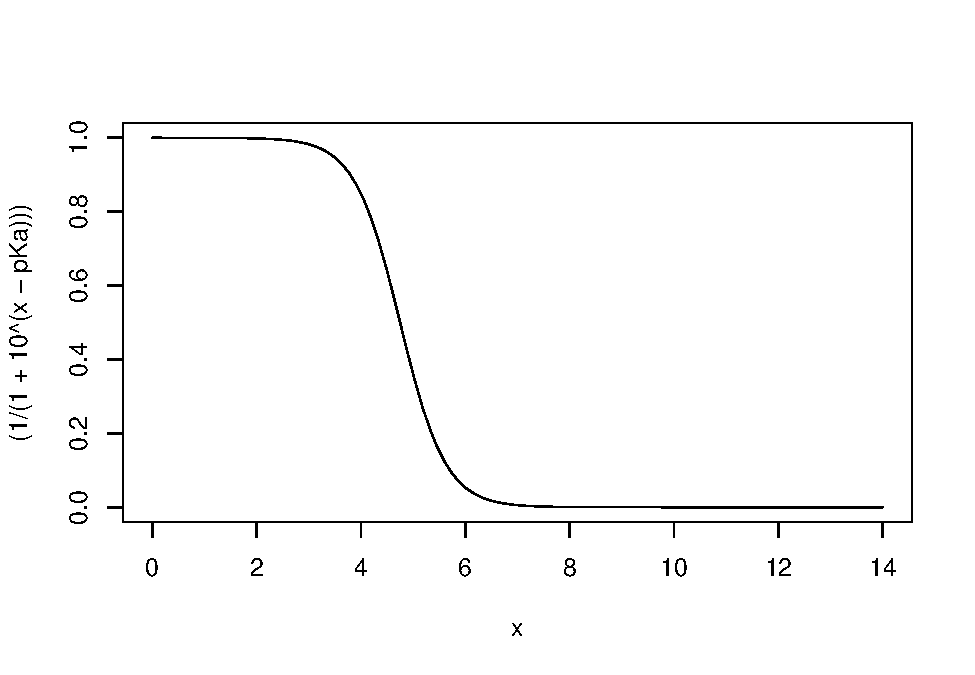
\includegraphics{Bioquímica-Quantitativa-com-R_files/figure-latex/unnamed-chunk-5-1.pdf}
\caption{\label{fig:unnamed-chunk-5}Relação entre pH (abscissa) e fração ácida (ordenada) para o par conjugado ácido acético/íon acetato.}
\end{figure}

~~Também pode-se fazer o inverso, elaborando um gráfico com a fração \emph{fb}:

\begin{lstlisting}[language=R]
# Curva de titulação para o sistema acetato/ácido acético
pKa = 4.75
curve(((10^(x-pKa))/(1+10^(x-pKa))),0,14)
\end{lstlisting}

\begin{figure}
\centering
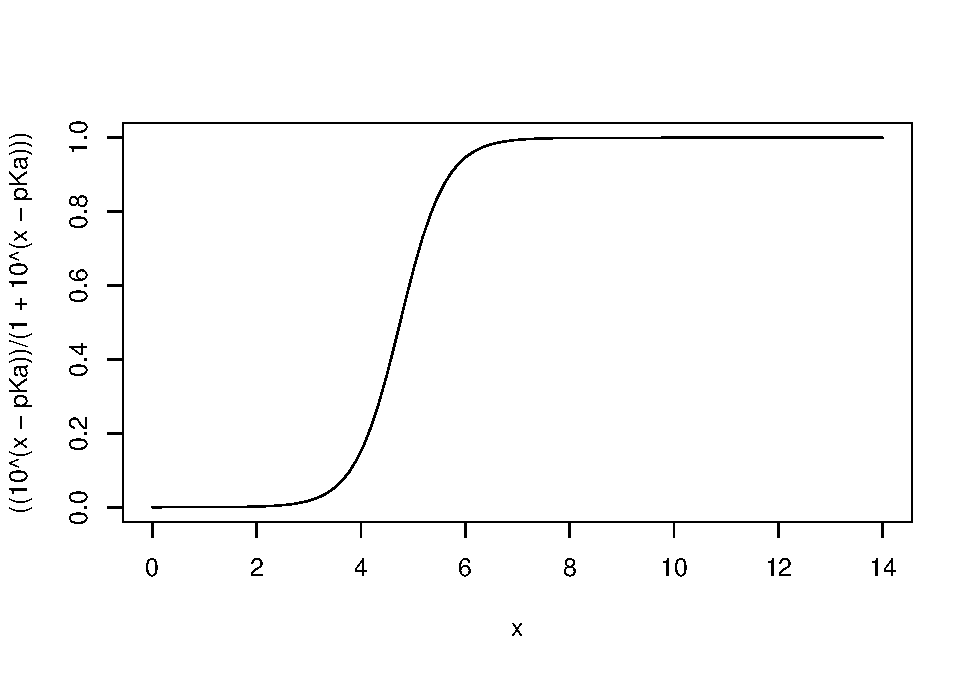
\includegraphics{Bioquímica-Quantitativa-com-R_files/figure-latex/unnamed-chunk-6-1.pdf}
\caption{\label{fig:unnamed-chunk-6}Relação entre pH (abscissa) e fração básica (ordenada) para o par conjugado ácido acético/íon acetato.}
\end{figure}

\hypertarget{sistema-bicarbonato}{%
\section{Sistema bicarbonato}\label{sistema-bicarbonato}}

~~~~~~Com o procedimento acima pode-se também simular a curva de titulação para o sistema bicarbonato de tamponamento sanguíneo com base nos valores de pKa do par ácido-base conjugado, apenas somando-se as expressões na Equação \eqref{eq:HH-fa}, tal que:

\begin{equation}
fa = \frac{1}{1+10^{(pH-pKa1)}}+ \frac{1}{1+10^{(pH-pKa2)}}
\label{eq:HHbic}
\end{equation}

Assim,

\begin{lstlisting}[language=R]
pKa1 = 6.37
pKa2 = 10.20
curve((1/(1+10^(x-pKa1)))+1/(1+10^(x-pKa2)),0,14)
\end{lstlisting}

\begin{figure}
\centering
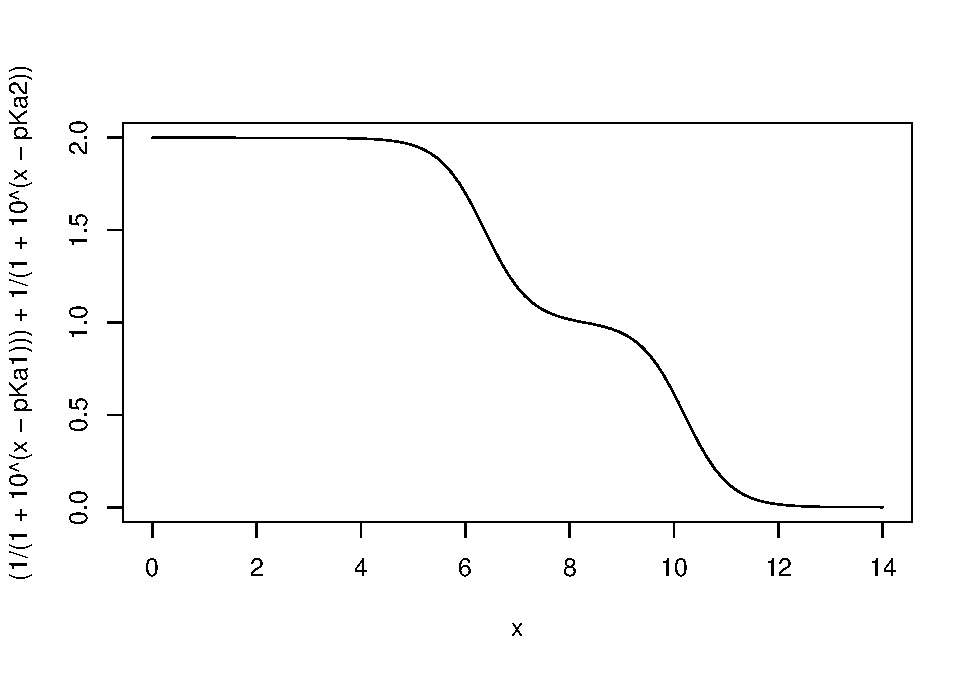
\includegraphics{Bioquímica-Quantitativa-com-R_files/figure-latex/titAcet-1.pdf}
\caption{\label{fig:titAcet}Relação entre pH (abscissa) e fração ácida (ordenada) para o par conjugado ácido carbônico/íon bicarbonato.}
\end{figure}

~~~~~~O gráfico da Figura \ref{fig:titAcet} pode ser armazenado em formatos, utilizando-se, por exemplo, o comando \passthrough{\lstinline!dev.copy!}:

\begin{lstlisting}[language=R]
dev.copy(pdf,"titBicarb.pdf",width=6, height=3) # alternativamente, bmp, jpeg, tiff, svg, png
\end{lstlisting}

~~~~~~E é claro que, partindo-se dos argumentos da função \passthrough{\lstinline!curve!} acima, e da flexibilidade que o pacote interno \emph{Graphics} do R possibilita, pode-se elaborar uma curva mais complexa, como segue:

\begin{lstlisting}[language=R]
pKa1 = 6.37
pKa2 = 10.20
curve((1/(1+10^(x-pKa1)))+1/(1+10^(x-pKa2)),0,14,
     xlab="pH",ylab="fa",
     main="Titulação de Ácido carbônico, H2CO3/HCO3-",
     type="o", n=50,lwd=2,lty="dotted",
     pch=3,col="blue",cex=1.2) # gráfico de titulação

text(4.7,1.3,"pKa = 6,37") # inserção de texto no gráfico
text(9,0.3,"pKa = 10,20")
abline(0.5,0, lty="dotted") # linha pontilhada em intercepto e inclinação específicos
abline(1.5,0, lty="dotted")
\end{lstlisting}

\begin{figure}
\centering
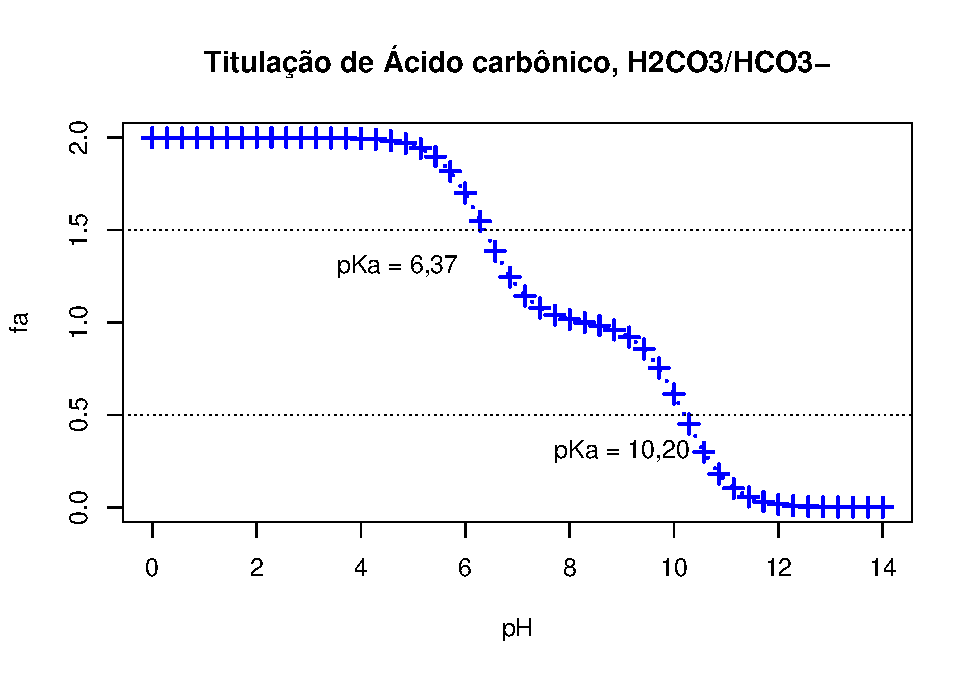
\includegraphics{Bioquímica-Quantitativa-com-R_files/figure-latex/unnamed-chunk-8-1.pdf}
\caption{\label{fig:unnamed-chunk-8}Variação de pH com redução da fração ácida em sistema bicarbonato.}
\end{figure}

~~~~~~A título de ilustração é possível ``recuperar'' o valor de \emph{pKa} fisiológico acima, ou seja, \emph{pKa1}, utilizando-se o comando \passthrough{\lstinline!locator()!}. Como trata-se de um ponto apenas no gráfico, basta digitar o código \passthrough{\lstinline!locator(1)!} e clicar com o botão esquerdo do mouse no ponto da curva correpondente à fração de 0,5 para \emph{fa}.

\begin{lstlisting}[language=R]
locator(1) # para mais pontos no gráfico, basta aumentar o valor entre parênteses
\end{lstlisting}

~~~~~~Observe que à medida em que o valor de \emph{pH} aproxima-se do de \emph{pKa}, a crescente variação em \emph{fa} parece afetar cada vez menos a variação em pH. Isto é a ``alma'' do sistema tampão, que permite aos organismos resistirem a variações de pH tanto quanto essas estiverem próximas do valor de \emph{pKa} correspondentes (bicarbonato, fosfato, proteínas).

~~~~~~Enquanto o sistema bicarbonato possui dois valores de pKa \footnote{Obs: o valor de pKa do sistema bicarbonato é de 6,8 quando considerado o \(CO_2\) como fonte de ácido carbônico \(H_2CO_3\) em sua reação com \(H_2O\), como por exemplo, para determinação de parâmetros arteriais em analisador hospitalar (\(CO_2\), \(HCO_3^-\), \(O_2\)).} , um dos quais na faixa de tamponamento fisiológico extracelular, o sistema fosfato que atua intracelularmente possui três valores de pKa, embora também atuando em apenas uma faixa fisiológica.

\hypertarget{sistema-fosfato}{%
\section{Sistema fosfato}\label{sistema-fosfato}}

~~~~~~Da mesma forma que simulado para o sistema bicarbonato, podemos elaborar uma curva de titulação para o sistema fosfato de tamponamento, dessa vez considerando seus três valores de pKa correspondentes a cada dissociação do ácido triprótico. Como dantes, a expressão que define a fração \emph{fa} deverá ser tomada como uma soma algébrica, como segue:

\begin{equation}
fa = \frac{1}{1+10^{(pH-pKa1)}}+ \frac{1}{1+10^{(pH-pK2)}}+\frac{1}{1+10^{(pH-pKa3)}}
\label{eq:HHfosf}
\end{equation}

No \emph{R} isso pode ser feito como abaixo:

\begin{lstlisting}[language=R]
pKa1=2.2
pKa2=7.2
pKa3=12.7

curve((1/(1+10^(x-pKa1)))+
      (1/(1+10^(x-pKa2)))+
      (1/(1+10^(x-pKa3))),
      xlim=c(1,14),
      xlab="pH",ylab="fa",
      main="Titulação de tampão fosfato",
      sub = " As linhas pontilhadas cruzam os valores de pKa"
                   )
abline(v=c(2.2,7.2,12.7),col=c("blue","red","green"),lty="dotted") # adição de linhas verticais marcando os valores de pKa
text(1.6,2.5,"pKa1") 
text(6.5,1.5,"pKa2")
text(11.8,0.5,"pKa3")
\end{lstlisting}

\begin{figure}
\centering
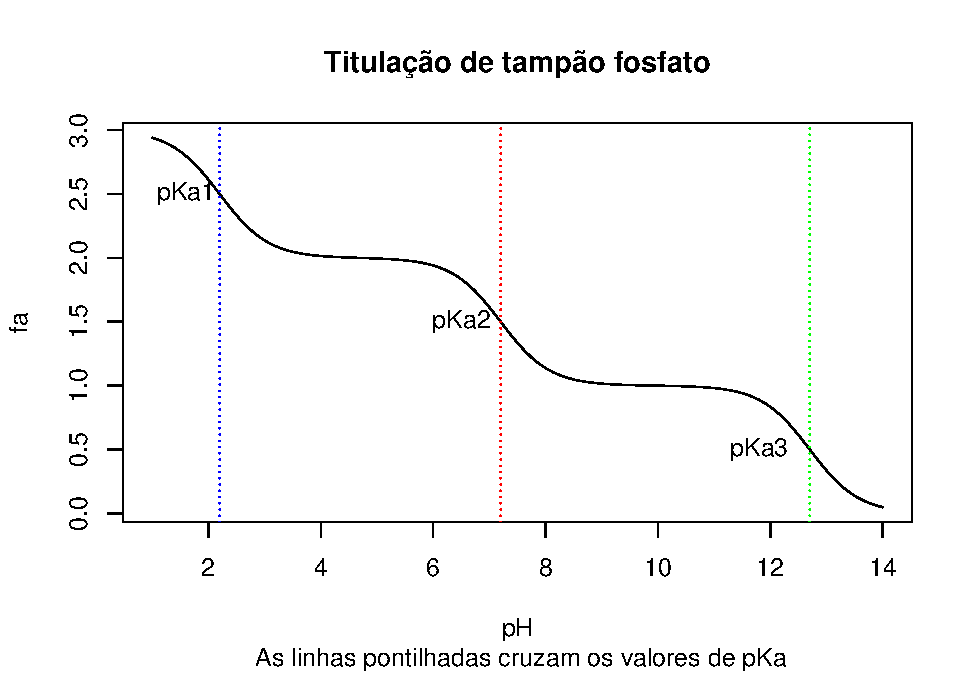
\includegraphics{Bioquímica-Quantitativa-com-R_files/figure-latex/unnamed-chunk-10-1.pdf}
\caption{\label{fig:unnamed-chunk-10}Curva de titulação em sistema fosfato de tamponamento.}
\end{figure}

\hypertarget{titulauxe7uxe3o-de-sistemas-em-geral-com-programauxe7uxe3o-do-r}{%
\subsection{Titulação de sistemas em geral com programação do R}\label{titulauxe7uxe3o-de-sistemas-em-geral-com-programauxe7uxe3o-do-r}}

~~Como ilustrado no fornecimento de argumentos da função \emph{args}, o `R' é uma linguagem de programação orientada a objeto, e cujos comandos são estruturados como \emph{funções}. Dessa forma, é possível criar uma função no `R' para operacionalizar ou automatizar qualquer trabalho computacional.\\
\hspace*{0.333em}\hspace*{0.333em}Uma função pode ser criada basicamente pelas instrução que segue:

\begin{lstlisting}[language=R]
função.X <- function( arg1, arg2, arg3 )
{
comandos de execução
return( objeto da função )
}
\end{lstlisting}

~~Como exemplo, pode-se criar uma função para converter a temperatura de graus Celsius (C) para temperatura absoluta (K), como segue:

\begin{lstlisting}[language=R]
# Função para conversão de graus Celsius a Kelvin
CtoK <- function (tC) {
  tK <-tC + 273.15
  return(tK)
  }
\end{lstlisting}

~~Para executar essa \emph{função CtoK}, basta:

\begin{lstlisting}[language=R]
# Executando CtoK:
CtoK (37)
\end{lstlisting}

\begin{lstlisting}
## [1] 310.15
\end{lstlisting}

~~Tendo isso em mente, também podemos criar uma função que auxilie na elaboração de curvas de titulação, como acima. Essas operações podem ser automatizadas não apenas para o tampão fosfato, mas para qualquer composto sob dissociação em meio aquoso, não importando o número de prótons envolvidos. Para isso, é necessário:

\begin{enumerate}
\def\labelenumi{\arabic{enumi}.}
\item
  Definir uma \emph{função} do \emph{R} que contenha os parâmetros e a operação desejada.
\item
  Incluir na função uma estrutura de \emph{laço} ou \emph{loop} que permita repetir a operação até exaurido o número de prótons do composto.
\item
  Definir um vetor do \emph{R} contendo os valores dos pKas do composto.
\item
  Definir a expressão de \emph{curva} que viabilize a simulação.
\end{enumerate}

Abaixo é apresentado um modelo de código que permite a simulação para o tampão fosfato.

\begin{lstlisting}[language=R]
#Define função e plot de titulação
fa = function(pH,pKa) {
  x=0
  for(i in 1:length(pKa)) {
    x = x+1/(1 + 10^(pH - pKa[i]))}
  return(x)
}
pKa=c(2.2,7.2,12.7)
curve(fa(x,pKa),1,14, xlab="pH", ylab="fa",
      col=2)
\end{lstlisting}

\begin{figure}
\centering
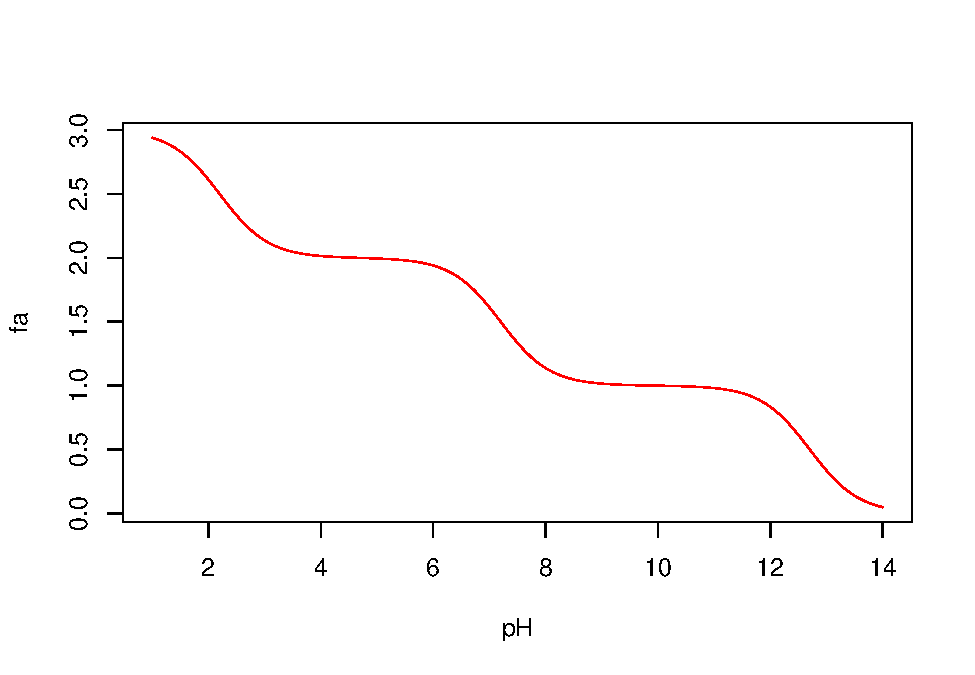
\includegraphics{Bioquímica-Quantitativa-com-R_files/figure-latex/unnamed-chunk-13-1.pdf}
\caption{\label{fig:unnamed-chunk-13}Curva de titulação para o tampão fosfato, tal como obtida por recurso de programação no R.}
\end{figure}

\hypertarget{AAcido}{%
\chapter{Aminoácidos \& Peptídios}\label{AAcido}}

\hypertarget{ponto-isoeluxe9trico-aminouxe1cidos}{%
\section{Ponto isoelétrico \& aminoácidos}\label{ponto-isoeluxe9trico-aminouxe1cidos}}

~~~~De modo geral o ponto isoelétrico, ou \emph{pI}, representa o valor de pH em que uma molécula adquire uma carga líquida nula sob campo elétrico, ou seja, suas cargas positivas anulam-se com as cargas negativas. Normalmente é experimentalmente obtido por medidas cinéticas, tais como \emph{potencial Zeta, eletrofocalização ou eletroforese capilar}. De modo similar, o \emph{ponto isoiônico} refere-se à mesma condição, no entanto na ausência de campo elétrico, podendo ser aferido por \emph{titulação potenciométrica, viscosidade}, ou pela informação estrutural de uma sequência monomérica, tal como ocorre na \emph{sequência primária de proteínas}.\\
\hspace*{0.333em}\hspace*{0.333em}Como todos os 20 aminoácidos que participam da estrutura proteica possuem grupos ionizáveis, tanto em seu esqueleto carbônico como em sua cadeia lateral, é possível prever o ponto isoiônico de um aminoácido em função dos valores de \emph{pKa} apresentados nesses grupos ionizáveis. O \emph{pI} também é denominado comumente por \emph{ponto isoelétrico}, embora essa definição encerre em si uma abrangência teórica mais complexa.

Exemplificando, o ácido glutâmico (Glu, E) apresenta um carboxilato ionizável em sua cadeia lateral, além dos grupos amina (-H\(_2\)N) e carboxilato do esqueleto carbônico (Figura \ref{fig:glu}):

\begin{figure}

{\centering 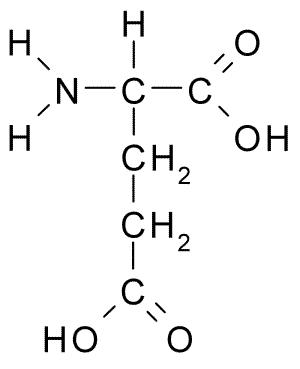
\includegraphics[width=0.2\linewidth]{figures/Glutamic_Acid} 

}

\caption{Fórmula estrutural planar para o ácido glutâmico (Wikimedia).}\label{fig:glu}
\end{figure}

~~~~Dessa forma, sua \emph{rede de carga líquida}, \emph{qnet}, pode ser determinada a partir da soma da forma ácida (qa) e básica (qb) da molécula, de forma similar como a que foi apresentada a partir da Equação \eqref{eq:HHfosf}:

\begin{equation}
qnet = qb + qa
\end{equation}
\label{eq:qnet}

\begin{equation}
qnet = qb+\frac{1}{1+10^{pH-pKa}}
\end{equation}
\label{eq:qnet2}

~~~~Como trata-se um ácido poliprótico, a equação \eqref{eq:qnet2} torna-se:

\begin{equation}
qnet = \sum_{i=1}^{n} {(qb+\frac{1}{1+10^{pH-pKi}})}
\end{equation}
\label{eq:qnet3}

, com \emph{pKi} como o enésimo valor de pKa. Dessa forma pode-se determinar programaticamente a curva de titulação do ácido glutâmico em função de sua carga, e não da fração ácida. Nessa linha, \emph{qb} representa a forma do composto em base, o que para Glu apresentará os valores de \emph{-1} para os dois carboxilatos, e de \emph{0} para o grupo amina, sendo necessário compor um vetor adicional para \emph{qb}.

\begin{lstlisting}[language=R]
#Titulação de Glu 

qNet = function(pH, qB, pKa) {
x=0
for(i in 1:length(qB)) {
x = x+qB[i] + 1/(1 + 10^(pH - pKa[i]))}
return(x)
}
 qB=c(-1,0,-1)
 pKa=c(2.2, 9.7, 4.3)

 curve(qNet(x,qB,pKa),1,12, xlab="pH", ylab="qNet")

abline(0,0,lty="dotted")
\end{lstlisting}

\begin{figure}
\centering
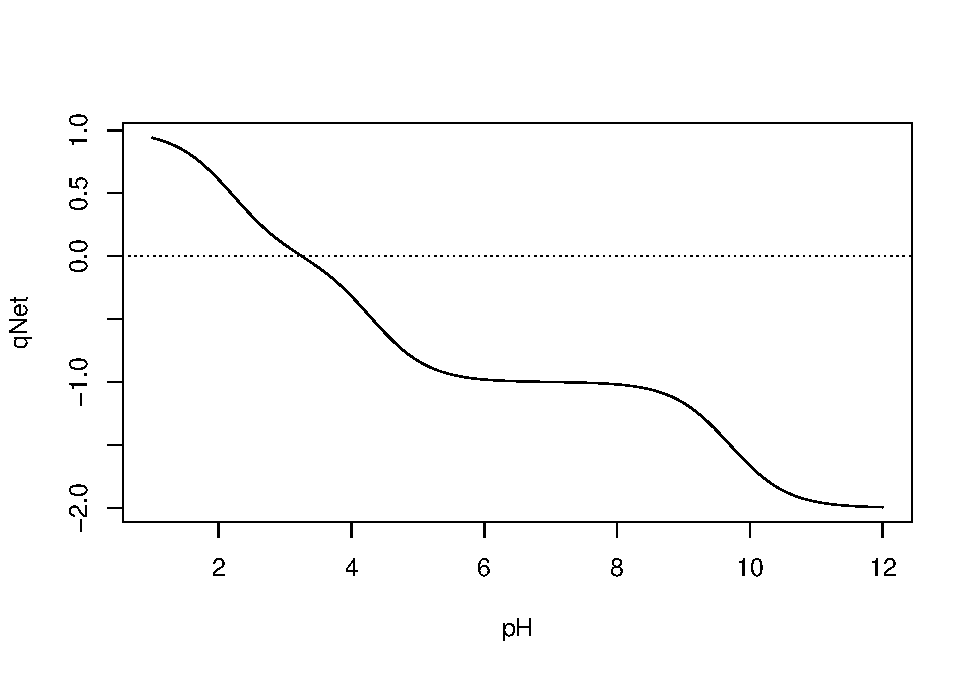
\includegraphics{Bioquímica-Quantitativa-com-R_files/figure-latex/unnamed-chunk-14-1.pdf}
\caption{\label{fig:unnamed-chunk-14}Curva de titulação para o ácido glutâmico. A curva intercepta a linha pontilhada no ponto isoiônico do Glu.}
\end{figure}

~~~~Manualmente é possível identificar o valor de \emph{pI} para o ácido glutâmico por uma função do \emph{R}, tal como \passthrough{\lstinline!locator()!} visto anteriormente. Mas também é possível acessar esse valor automaticamente, aplicando um comando que encontre a raíz dessa função, ou seja, o valor de pH que corresponda a um valor nulo para \emph{qnet}. Para isto, exemplifica-se o uso de \passthrough{\lstinline!uniroot!}, no qual define-se a função matemática pretendida, bem como os limites inferior e superior para a busca pelo algoritmo, como segue:

\begin{lstlisting}[language=R]
 #Cálculo de pI
 f=function(pH) {qNet(pH,qB,pKa)}
str(uniroot(f,c(2,5)))
\end{lstlisting}

\begin{lstlisting}
## List of 5
##  $ root      : num 3.25
##  $ f.root    : num -4.8e-06
##  $ iter      : int 4
##  $ init.it   : int NA
##  $ estim.prec: num 6.1e-05
\end{lstlisting}

~~~~Esse resultado traduz-se como um pI de 3,25 (\passthrough{\lstinline!root!}), em 4 iterações, com uma estimativa de precisão de 6,1x10\^{}\{-5\}, e erro associado de -4,8x10\^{}\{-6\}.\\
\hspace*{0.333em}\hspace*{0.333em}\hspace*{0.333em}\hspace*{0.333em}Essa forma de se obter um valor empregando-se o cálculo numérico é por vezes denominada \textbf{solução numérica}. Por outro lado, pode-se obter o valor de pI para o Glu por um procedimento mais simples, normalmente encontrado nos livros-texto sobre o assunto, e que assume a forma abaixo:

\begin{equation}
pI = \frac{pKa1+pKa2}{2}
\end{equation}

~~~~No nosso exemplo, o pI envolverá os pKas dos dois carboxilatos, o que resultará em \emph{(2,3+4,2)/2}, ou seja, \emph{3,25} ! Nada mal para uma aproximação, não ? Esse procedimento envolvendo a solução de um problema matemático a partir de parâmetros do sistema é denominado método ou \textbf{solução analítica}. Essa solução também pode ser exemplificada pelo parâmetro obtido em função da observação do comportamento gráfico da titulação, como nas figuras acima.

~~~Agora, pra que nos serve um procedimento numérico mais complexo, se uma simples equação analítica já nos resolve o problema de se encontrar o valor de pI para o ácido glutâmico ? Bom, extamente pra isso, para solução de problemas mais complexos. Um pouco menos retórico, entretanto, pode-se afirmar que a \emph{solução numérica} funciona melhor para sistemas onde a \emph{solução analítica} por vezes não é suficiente ou torna-se mesmo impossível, como na solução de equações com dezenas de parâmetros.

\hypertarget{ponto-isoiuxf4nico-biopoluxedmeros}{%
\section{Ponto isoiônico \& biopolímeros}\label{ponto-isoiuxf4nico-biopoluxedmeros}}

~~Uma situção nesse tema pode ser ilustrada pela obtenção do valor de pI para uma proteína. Exemplificando, a lisozima humana, enzima de estrutura terciária composta por 130 resíduos de aminoácidos. Nesse caso, a \emph{solução analítica} esbarra na complexidade em se identificar quais desses resíduos são ionizáveis em solução aquosa, e quais estariam envolvidos numa distribuição que resultasse numa carga líquida nula para a molécula.

~~Para esse sistema mais complexo é necessário ampliar um pouco a função definida para o ácido glutâmico, computando-se no vetor de \emph{qb} as cargas em base dos 7 aminoácidos com cadeias laterais ionizáveis, e atribuir um novo vetor para o quantitativo de cada resíduo ionizável presente na lisozima. O código abaixo exemplifica essa solução, calcula o pI da enzima, e elabora o gráfico de sua titulação, embora essa ordem não seja relevante, posto que o pI é calculado numericamente, e não graficamente.

\begin{lstlisting}[language=R]
 # Titulação de Lisozima e Determinação de pI

 #Define função para qNet
qNet = function(pH, qB, pKa, n) {
x=0
for(i in 1:length(qB)) {
x = x+n[i]*qB[i] + n[i]/(1 + 10^(pH - pKa[i]))}
return(x)
}

# Define pKas de aCOOH, aNH3 e as 7 cadeias laterais de AA
pKa=c(2.2, 9.6, 3.9, 4.1, 6.0, 8.5, 10.1, 10.8, 12.5)

# Define qB, as cargas de cada aminoácido na forma básica
qB =c(-1, 0, -1, -1, 0, -1, -1, 0, 0)

ionizavel=c("aCOOH","aNH3","Asp","Glu","His","Cys","Tyr",
"Lys","Arg")
n=c(1,1,7,3,1,8,6,5,14) # Lista para quantidades de resíduos ionizáveis na lisozima (cada elemento representa a quantidade de aCOOH, aNH3, e determinado AA na enzima)

# Cálculo de pI 
f=function(pH) {qNet(pH,qB,pKa,n)} 
str(uniroot(f,c(1,13))) # estimativa de pI entre 10 e 12
\end{lstlisting}

\begin{lstlisting}
## List of 5
##  $ root      : num 9.46
##  $ f.root    : num 3.3e-07
##  $ iter      : int 7
##  $ init.it   : int NA
##  $ estim.prec: num 6.1e-05
\end{lstlisting}

\begin{lstlisting}[language=R]
# Gráfico de titulação 
curve(qNet(x,qB,pKa,n),1,12, xlab="pH", ylab="qNet")
abline(0,0,lty=3)
\end{lstlisting}

\begin{figure}
\centering
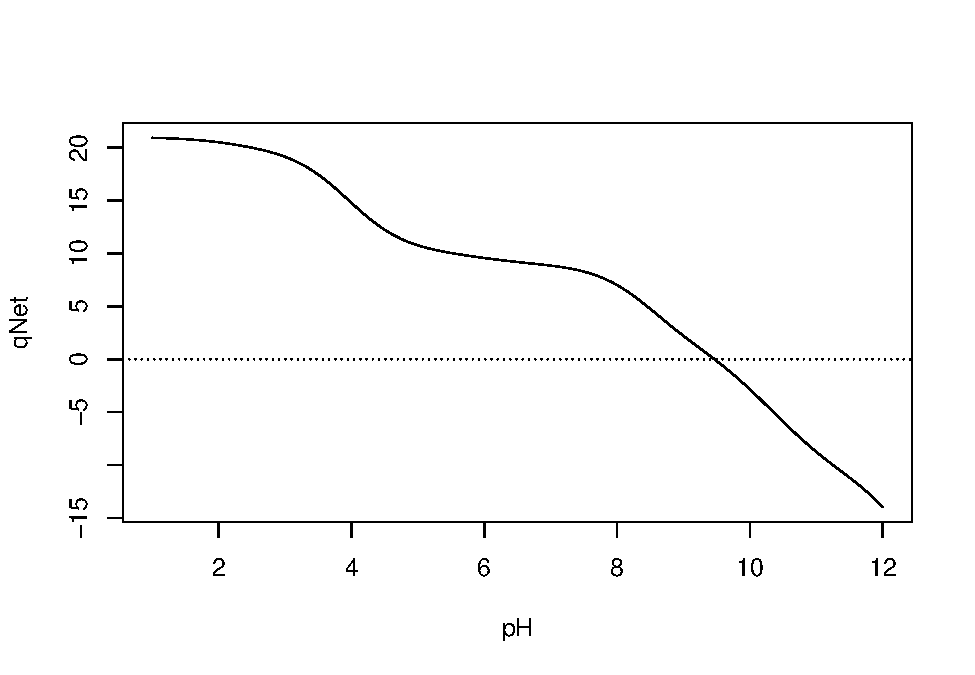
\includegraphics{Bioquímica-Quantitativa-com-R_files/figure-latex/unnamed-chunk-16-1.pdf}
\caption{\label{fig:unnamed-chunk-16}Curva de titulação para lisozima.}
\end{figure}

~~~Observe que o valor encontrado para pI da lisozima foi de 9,46; ou seja, em pH 9,46 a enzima apresenta rede de carga líquida nula, como também pode ser verificado na representação gráfica.

\hypertarget{ponto-isoiuxf4nico-bibliotecas-do-r}{%
\section{Ponto isoiônico \& bibliotecas do R}\label{ponto-isoiuxf4nico-bibliotecas-do-r}}

~~Não obstante a precisão do cálculo de pI pela \emph{solução numérica} realizada para a lisozima, uma das características mais fascinantes do programa reside no uso de bibliotecas (\passthrough{\lstinline!packages!}), não sendo diferente para determinção de propriedades de biopolímeros, tais como pI.\\
\hspace*{0.333em}\hspace*{0.333em}Entre as bibliotecas existentes para propriedades físico-químicas de proteínas e ácidos nucleicos exemplifica-se o pacote \passthrough{\lstinline!seqinr!}, \emph{Biological Sequences Retrieval and Analysis} \footnote{Pacote seqinr: \url{https://cran.r-project.org/web/packages/seqinr/index.html}}, de análise e visualização exploratória de biopolímeros. Para uso desse pacote, contudo, faz-se necessário a obtenção da sequência primária da proteína, representada em código de uma letra. Pode-se obter a sequência primária da lisozima pelo sítio do \emph{National Center for Biotechnology Information}, NCBI \footnote{NCBI. \url{https://www.ncbi.nlm.nih.gov/protein}}. Um truque rápido envolve:

\begin{enumerate}
\def\labelenumi{\arabic{enumi})}
\item
  digitar o nome da proteína;
\item
  selecionar entre as opções resultantes;
\item
  clicar em FASTA para obter a sequência primária de 1 letra.
\item
  copiar a sequência da proteína apresentada para o \passthrough{\lstinline!seqinr!}.
\end{enumerate}

~~Presupondo-se que a biblioteca \passthrough{\lstinline!seqinr!} esteja instalada, e que a sequência tenha sido obtida para a lisozima (busca por \emph{CAA32175} ou \emph{lysozyme {[}Homo sapiens{]}}), pode-se encontrar o valor do pI para a mesma pelo código que segue:

\begin{lstlisting}[language=R]
library(seqinr)
lisozima<-s2c("KVFERCELARTLKRLGMDGYRGISLANWMCLAKWESGYNTRATNYNAGDR STDYGIFQINSRYWCNDGKTPGAVNACHLSCSALLQDNIADAVACAKRVV RDPQGIRAWVAWRNRCQNRDVRQYVQGCGV") # converte sequência de string em vetor de caracteres
computePI(lisozima)
\end{lstlisting}

\begin{lstlisting}
## [1] 9.2778
\end{lstlisting}

~~~Veja que o valor de pI pelo pacote, 9,28, foi bem próximo do encontrado pela \emph{solução numérica} acima. Isto deve-se ao uso de algoritmos distintos para ambos, bem como o cômputo dos valores de pKa distintos para o \passthrough{\lstinline!seqinr!}. Exemplificando essa variação, o próprio \passthrough{\lstinline!seqinr!} apresenta valores de pKa diferentes, em função da base de dados buscada. Para verificar isso, digite o comando abaixo e visualize e variável \emph{pK} resultante.

\begin{lstlisting}[language=R]
library(seqinr)
data(pK)
\end{lstlisting}

~~~~Complementarmente, pode-se também comparar o valor de pI da lisozima com o algoritmo utilizado pelo banco de dados no sítio \footnote{Expasy. \url{https://web.expasy.org/compute_pi/}}. Para isto, basta colar a sequência de resíduos no campo disponível e clicar o cômputo de pI. Veja que o valor resultante de 9,28 coincide com o do algoritmo utilizado pelo pacote \passthrough{\lstinline!seqinr!} do R.

\begin{lstlisting}[language=R]
library(knitr)
knitr::kable(pK, "pipe", caption = "Tabela de valores de pKa para aminoácidos a partir de diversas fontes, extraída do pacote seqinr.")
\end{lstlisting}

\begin{longtable}[]{@{}lrrrrrr@{}}
\caption{\label{tab:unnamed-chunk-19}Tabela de valores de pKa para aminoácidos a partir de diversas fontes, extraída do pacote seqinr.}\tabularnewline
\toprule
& Bjellqvist & EMBOSS & Murray & Sillero & Solomon & Stryer \\
\midrule
\endfirsthead
\toprule
& Bjellqvist & EMBOSS & Murray & Sillero & Solomon & Stryer \\
\midrule
\endhead
C & 9.00 & 8.5 & 8.33 & 9.0 & 8.3 & 8.5 \\
D & 4.05 & 3.9 & 3.68 & 4.0 & 3.9 & 4.4 \\
E & 4.45 & 4.1 & 4.25 & 4.5 & 4.3 & 4.4 \\
H & 5.98 & 6.5 & 6.00 & 6.4 & 6.0 & 6.5 \\
K & 10.00 & 10.8 & 11.50 & 10.4 & 10.5 & 10.0 \\
R & 12.00 & 12.5 & 11.50 & 12.0 & 12.5 & 12.0 \\
Y & 10.00 & 10.1 & 10.07 & 10.0 & 10.1 & 10.0 \\
\bottomrule
\end{longtable}

~~~~Existem outros pacotes do R que analisam sequências de aminoácidos e nucleotídeos, incluindo o cálculo de pI, entre os quais vale mencionar o Peptides \footnote{pacote Peptides. \url{https://cran.r-project.org/web/packages/Peptides/index.html}}.

\hypertarget{Proteinas}{%
\chapter{Proteínas}\label{Proteinas}}

\hypertarget{composiuxe7uxe3o-de-aminouxe1cidos}{%
\section{Composição de aminoácidos}\label{composiuxe7uxe3o-de-aminouxe1cidos}}

~~~~Proteínas constituem biopolímeros formados por 20 aminoácidos. Dessa forma pode-se avaliar facilmente a composição de qualquer proteína disponível em banco de dados, como o \emph{PDB} visto no capítulo \ref{AAcido}. Tomando-se a albumina de soro humano como exemplo, código \emph{AAA98797} do \emph{National Center for Biotechnology Information}, é possível contabilizar os 20 tipos de aminoácidos que compõe sua sequência. Para isto basta considerar a sequência \emph{FASTA} como uma \emph{string}, e extrair a quantidade de cada letra, utilizando-se a biblioteca \emph{stringr}, como segue.

~~~~Primeiro, obtém-se a sequência \emph{FASTA} da albumina de soro.

\begin{lstlisting}[language=R]
seq<-"MKWVTFISLLFLFSSAYSRGVFRRDAHKSEVAHRFKDLGEENFKALVLIAFAQYLQQCPFEDHVKLVNEV
TEFAKTCVADESAENCDKSLHTLFGDKLCTVATLRETYGEMADCCAKQEPERNECFLQHKDDNPNLPRLV
RPEVDVMCTAFHDNEETFLKKYLYEIARRHPYFYAPELLFFAKRYKAAFTECCQAADKAACLLPKLDELR
DEGKASSAKQRLKCASLQKFGERAFKAWAVARLSQRFPKAEFAEVSKLVTDLTKVHTECCHGDLLECADD
RADLAKYICENQDSISSKLKECCEKPLLEKSHCIAEVENDEMPADLPSLAADFVESKDVCKNYAEAKDVF
LGMFLYEYARRHPDYSVVLLLRLAKTYETTLEKCCAAADPHECYAKVFDEFKPLVEEPQNLIKQNCELFE
QLGEYKFQNALLVRYTKKVPQVSTPTLVEVSRNLGKVGSKCCKHPEAKRMPCAEDYLSVVLNQLCVLHEK
TPVSDRVTKCCTESLVNRRPCFSALEVDETYVPKEFNAETFTFHADICTLSEKERQIKKQTALVELVKHK
PKATKEQLKAVMDDFAAFVEKCCKADDKETCFAEEGKKLVAASQAALGL"
\end{lstlisting}

~~~~Pode-se observar que há espaços vazios, que podem ser omitidos por razões estéticas ou não, já que o pacote \emph{stringr} não os contabilizará, contrariamente a pacotes mais específicos para sequências biológicas, como o \emph{seqinr} visto anteriormente. Mas se desejar omitir esses espaços, basta executar o código abaixo.

\begin{lstlisting}[language=R]
seq<-seq[seq !="\n"]; seq # operação booleana != significa "não"
\end{lstlisting}

\begin{lstlisting}
## [1] "MKWVTFISLLFLFSSAYSRGVFRRDAHKSEVAHRFKDLGEENFKALVLIAFAQYLQQCPFEDHVKLVNEV\nTEFAKTCVADESAENCDKSLHTLFGDKLCTVATLRETYGEMADCCAKQEPERNECFLQHKDDNPNLPRLV\nRPEVDVMCTAFHDNEETFLKKYLYEIARRHPYFYAPELLFFAKRYKAAFTECCQAADKAACLLPKLDELR\nDEGKASSAKQRLKCASLQKFGERAFKAWAVARLSQRFPKAEFAEVSKLVTDLTKVHTECCHGDLLECADD\nRADLAKYICENQDSISSKLKECCEKPLLEKSHCIAEVENDEMPADLPSLAADFVESKDVCKNYAEAKDVF\nLGMFLYEYARRHPDYSVVLLLRLAKTYETTLEKCCAAADPHECYAKVFDEFKPLVEEPQNLIKQNCELFE\nQLGEYKFQNALLVRYTKKVPQVSTPTLVEVSRNLGKVGSKCCKHPEAKRMPCAEDYLSVVLNQLCVLHEK\nTPVSDRVTKCCTESLVNRRPCFSALEVDETYVPKEFNAETFTFHADICTLSEKERQIKKQTALVELVKHK\nPKATKEQLKAVMDDFAAFVEKCCKADDKETCFAEEGKKLVAASQAALGL"
\end{lstlisting}

A seguir, obtém-se o quantitativo de uma letra específica da sequência.

\begin{lstlisting}[language=R]
library(stringr)
aa<-str_count(seq, pattern="A"); aa
\end{lstlisting}

\begin{lstlisting}
## [1] 63
\end{lstlisting}

~~~~Veja que o comando \passthrough{\lstinline!str\_count!} contabiliza apenas a letra ``A'' na sequência. Dessa forma, é possível obter todos os 20 aminoácidos, repetindo-se esse comando.

\begin{lstlisting}[language=R]
library(stringr)
ala<-str_count(seq, pattern="A")
arg<-str_count(seq, pattern="R")
asn<-str_count(seq, pattern="N")
asp<-str_count(seq, pattern="D")
cys<-str_count(seq, pattern="C")
glu<-str_count(seq, pattern="E")
gln<-str_count(seq, pattern="Q")
gly<-str_count(seq, pattern="G")
his<-str_count(seq, pattern="H")
ile<-str_count(seq, pattern="I")
leu<-str_count(seq, pattern="L")
lys<-str_count(seq, pattern="K")
met<-str_count(seq, pattern="M")
phe<-str_count(seq, pattern="F")
pro<-str_count(seq, pattern="P")
ser<-str_count(seq, pattern="S")
thr<-str_count(seq, pattern="T")
trp<-str_count(seq, pattern="W")
tyr<-str_count(seq, pattern="Y")
val<-str_count(seq, pattern="V")
\end{lstlisting}

E, para visualizar o resultado numa tabela:

\begin{lstlisting}[language=R]
aa_3abrev<-c("Ala","Arg","Asn","Asp","Cys","Glu","Gln","Gly","His","Ile","Leu","Lys","Met","Phe","Pro","Ser","Thr","Trp","Tyr","Val") # vetor com os nomes de cada aminoácido
aa_quant<-c(ala,arg,asn,asp,cys,glu,gln,gly,his,ile,leu,lys,met,phe,pro,ser,thr,trp,tyr,val) # vetor com o quantitativo de aminoácidos da proteína
aa_seq<-data.frame(aa_3abrev,aa_quant) # dataframe com os resultados
colnames(aa_seq)<-c("Tipo","Qtde") # renomear as colunas


# Composição de aminoácidos em albumina de soro humano
aa_seq # apresenta a tabela
\end{lstlisting}

\begin{lstlisting}
##    Tipo Qtde
## 1   Ala   63
## 2   Arg   27
## 3   Asn   17
## 4   Asp   36
## 5   Cys   35
## 6   Glu   62
## 7   Gln   20
## 8   Gly   13
## 9   His   16
## 10  Ile    9
## 11  Leu   64
## 12  Lys   60
## 13  Met    7
## 14  Phe   35
## 15  Pro   24
## 16  Ser   28
## 17  Thr   29
## 18  Trp    2
## 19  Tyr   19
## 20  Val   43
\end{lstlisting}

~~~~~~O `R' possui alguns comandos para a geração estética de tabelas, entre os quais os incluídos no pacote `knitr', como segue:

\begin{lstlisting}[language=R]
library(knitr) # para gerar a tabela

knitr::kable(aa_seq, caption="Composição de aminoácidos em albumina de soro humano.", "pipe") # tabela
\end{lstlisting}

\begin{longtable}[]{@{}lr@{}}
\caption{\label{tab:unnamed-chunk-23}Composição de aminoácidos em albumina de soro humano.}\tabularnewline
\toprule
Tipo & Qtde \\
\midrule
\endfirsthead
\toprule
Tipo & Qtde \\
\midrule
\endhead
Ala & 63 \\
Arg & 27 \\
Asn & 17 \\
Asp & 36 \\
Cys & 35 \\
Glu & 62 \\
Gln & 20 \\
Gly & 13 \\
His & 16 \\
Ile & 9 \\
Leu & 64 \\
Lys & 60 \\
Met & 7 \\
Phe & 35 \\
Pro & 24 \\
Ser & 28 \\
Thr & 29 \\
Trp & 2 \\
Tyr & 19 \\
Val & 43 \\
\bottomrule
\end{longtable}

~~~~Observe que, à despeito do resultado obtido, houve certo trabalho em se obter a composição da albumina, a partir das 20 linhas modificadas para cada aminoácido. Uma alternativa mais prática consiste em considerar um \emph{loop} que execute a extração da informação desejada para um vetor contendo a abreviação de uma letra para cada aminoácido.

\begin{lstlisting}[language=R]
aa_1abrev=c("A","R","N","D","C","E","Q","G","H", "I","L","K", "M","F","P","S","T","W","Y","V")
for(i in aa_1abrev) {
  aa_quant2<-str_count(seq, pattern=aa_1abrev)
  return(aa_quant2)  # sintaxe opcional para função com apenas uma saída
}


aa_seq<-data.frame(aa_3abrev,aa_quant2) # dataframe com os resultados
colnames(aa_seq)<-c("Tipo","Qtde") # renomear as colunas
knitr::kable(aa_seq,caption="Composição de aminoácidos em albumina de soro humano (uso de loop).", "pipe") # tabela
\end{lstlisting}

\begin{longtable}[]{@{}lr@{}}
\caption{(\#tab:loop table bsa)Composição de aminoácidos em albumina de soro humano (uso de loop).}\tabularnewline
\toprule
Tipo & Qtde \\
\midrule
\endfirsthead
\toprule
Tipo & Qtde \\
\midrule
\endhead
Ala & 63 \\
Arg & 27 \\
Asn & 17 \\
Asp & 36 \\
Cys & 35 \\
Glu & 62 \\
Gln & 20 \\
Gly & 13 \\
His & 16 \\
Ile & 9 \\
Leu & 64 \\
Lys & 60 \\
Met & 7 \\
Phe & 35 \\
Pro & 24 \\
Ser & 28 \\
Thr & 29 \\
Trp & 2 \\
Tyr & 19 \\
Val & 43 \\
\bottomrule
\end{longtable}

~~~~Dessa forma obtém-se o mesmo resultado, mas com menor consumo de memória e maior velocidade de processamento, características em qualquer lógica de programação. Apesar do \emph{loop} exemplificar uma automação, a função \passthrough{\lstinline!str\_count!} retém em si um \emph{loop} interno, já que aplica uma função de contagem de elementos a uma sequência, a partir de um padrão pré-definido (o vetor \emph{aa\_1abrev}, no caso). Dessa forma, pode-se simplificar ainda mais o script, não necessitando do \emph{loop} externo.

\begin{lstlisting}[language=R]
str_count(seq, pattern=aa_1abrev)
\end{lstlisting}

\begin{lstlisting}
##  [1] 63 27 17 36 35 62 20 13 16  9 64 60  7 35 24 28 29  2 19 43
\end{lstlisting}

~~~~Diversas funções do R exibem esse \emph{loop} interno, e que pode ser aplicado em vetores, listas, matrizes e \emph{dataframes} (planilha de dados). As mais simples envolvem a aplicação de uma função pré-programada do R a um vetor, por ex:

\begin{lstlisting}[language=R]
y=c(1,2,4,8,16,32)
mean(y)
\end{lstlisting}

\begin{lstlisting}
## [1] 10.5
\end{lstlisting}

\begin{lstlisting}[language=R]
sum(y)
\end{lstlisting}

\begin{lstlisting}
## [1] 63
\end{lstlisting}

~~~~~~Outra vetorização frequente decorre da aplicação de uma \emph{função} de usuário a vetor, reduzindo a necessidade de repetição de comandos, como no exemplo abaixo:

\begin{lstlisting}[language=R]
# Tamanho médio estimado de uma proteína a partir do no. de resíduos de aminoácidos
prot.tamanho<-function(x){ 
  MM<-x*110 # 'x' representa o número de aminoácidos da proteína
return(MM)
}

prot.tamanho(575) # no. de resíduos de aminoácidos de albumina humana
\end{lstlisting}

\begin{lstlisting}
## [1] 63250
\end{lstlisting}

~~~~~~Outra forma de vetorização envolve a família de funções \passthrough{\lstinline!apply!}, composta pelos comandos \passthrough{\lstinline!apply!}, \passthrough{\lstinline!sapply!}, \passthrough{\lstinline!tapply!}, \passthrough{\lstinline!lapply!}, e \passthrough{\lstinline!mapply!}. Embora possuam processamento mais rápido que funções de \emph{loop} externo para uso de matrizes muito complexas, cada qual é voltado a um objeto distinto ou situação específica do R (retorno de lista, vetor ou matriz), permite o uso de \passthrough{\lstinline!subset!} (subconjuntos de dados), utiliza funções do R ou funções previamente definidas pelo usuário, e roda em apenas uma linha de comando. Essas vantagens contrapõe-se ao uso de \emph{loop for} aplicado para vetores. Contudo, a vetorização opera muito bem quando se deseja aplicar ou mapear uma função a um vetor/matriz/lista. Quando, por outro lado, se deseja aplicar uma função cujo resultado dependa de mais de um vetor/matriz/lista, o \emph{loop for} torna-se indispensável, como na titulação de ácidos fracos do capítulo \ref{AAcido}.

~~~~Seja qual for o método empregado (e aí vale destacar as chamadas \emph{boas práticas de programação} na construção de \emph{scripts} \footnote{Algumas práticas de programação (\emph{Best Codes}):
  1) organizar um projeto em pastas (ex: dados,figuras,scripts) ou criar um pacote do R como opção; 2) criar seções num código pra facilitar localização; 3) nomear os \emph{code chunks} (pedaços de código); 4) colocar no início do código as bibliotecas utilizadas, fontes, e chamada de dados (evita procurar algo necessário pro \emph{script} rodar ao longo do código); 5) identar, preferivelmente com 1 ou 2 comandos por linha; 6) parâmetros de função sempre dentro de função; 7) evitar parâmetros globais; 8) não usar `attach'; 8) usar parâmetros com nomes intuitivos (e não x e y; ex: nome\_função); 9) atribuir nomes à objetos com uma das três convenções nominais (ex: KiCompet, ki\_compet, ki.compet).}), é possível construir uma composição mais geral para o conjunto de resíduos da proteína. Assim, podemos obter qualquer relação quantitativa a partir da sequência, já que a estamos tratando como uma \emph{string}. Exemplificando, uma tabela contendo a classe de cada aminoácido que compõe a sequência.

\begin{lstlisting}[language=R]
aa_ac<-aa_seq[4,2]+aa_seq[6,2] # AA ácicos
aa_bas<-aa_seq[2,2]+aa_seq[9,2]+aa_seq[12,2] # AA básicos
aa_arom<-aa_seq[14,2]+aa_seq[18,2]+aa_seq[19,2] # AA aromáticos
aa_alif<-aa_seq[10,2]+aa_seq[11,2]+aa_seq[15,2]+aa_seq[1,2]+aa_seq[20,2] # AA alifáticos
aa_pol<-aa_seq[3,2]+aa_seq[5,2]+aa_seq[7,2]+aa_seq[8,2]+aa_seq[13,2]+aa_seq[16,2]+aa_seq[17,2] ## AA polares neutros
\end{lstlisting}

~~~~Agora, ao invés de se construir uma tabela com a contagem desses grupos, façamos o percentual dos mesmos, para uma visão mais geral da sequência.

\begin{lstlisting}[language=R]
aa_tot<-str_count(seq,pattern="") # comprimento da sequência
class_perc<-round(c(aa_ac,aa_bas,aa_arom,aa_alif,aa_pol)/aa_tot*100)
\end{lstlisting}

E agora, sim, constroi-se a tabela.

\begin{lstlisting}[language=R]
aa_class<-c("ácido","básico","aromático","alifático","polar")
aa_perc<-data.frame(aa_class,class_perc) # dataframe com os resultados
colnames(aa_perc)<-c("Classe","%") # renomear as colunas
knitr::kable(aa_perc, caption="Distribuição de classes de aminoácidos em albumina humana.", "pipe") # tabela
\end{lstlisting}

\begin{longtable}[]{@{}lr@{}}
\caption{\label{tab:unnamed-chunk-28}Distribuição de classes de aminoácidos em albumina humana.}\tabularnewline
\toprule
Classe & \% \\
\midrule
\endfirsthead
\toprule
Classe & \% \\
\midrule
\endhead
ácido & 16 \\
básico & 17 \\
aromático & 9 \\
alifático & 33 \\
polar & 24 \\
\bottomrule
\end{longtable}

~~~~Percebe-se pela tabela acima que a distribuição de classes de resíduos de aminoácidos na albumina é razoavelmente homogênea, o que contribui para sua função anfotérica de transporte para compostos polares (ex:cálcio) e apolares (ex: colesterol, ácidos graxos).

\hypertarget{tabela-de-purificauxe7uxe3o-de-proteuxednas-r-como-planilha-eletruxf4nica}{%
\section{Tabela de Purificação de Proteínas \& R como planilha eletrônica}\label{tabela-de-purificauxe7uxe3o-de-proteuxednas-r-como-planilha-eletruxf4nica}}

~~~~~Não obstante a facilidade com que podemos elaborar/editar planilhas eletrônicas convencionais (\emph{spreadsheet}; ex: MS Excel, Libreoffice Calc, Gnumeric, etc), o `R' também permite trabalhar-se com planilhas. Ainda que menos intuitivo como as mencionadas, a scriptagem no R permite a elaboração/edição de planilhas de alta complexidade, dada a natureza da programação estatística que envolve a suite.\\
\hspace*{0.333em}\hspace*{0.333em}\hspace*{0.333em}\hspace*{0.333em}\hspace*{0.333em}\hspace*{0.333em}Para exemplificar a construção de uma planilha simples, tomemos como exemplo uma \emph{Tabela de Purificação de Proteínas}, usualmente utilizada em Biotecnologia e áreas afins. A forma mais simples de construção de uma planilha envolve 1) a elaboração individual de vetores, e 2) a união dos vetores em uma planilha.\\
\hspace*{0.333em}\hspace*{0.333em}\hspace*{0.333em}\hspace*{0.333em}\hspace*{0.333em}\hspace*{0.333em}Os procedimentos para purificação (ou isolamento, fracionamento) proteica envolvem técnicas como \textbf{tratamento químico (precipitação por sulfato de amônio, acetona)}, \textbf{tratamento ácido}, \textbf{tratamento térmico}, \textbf{diálise}, \textbf{cromatografia (filtração molecular, troca-iônica, afinidade, fase reversa)}, entre outros. Para aferição do grau de pureza da amostra obtida utilizam-se normalmente a \textbf{eletroforese} simples, \textbf{focalização isoelétrica}, \textbf{eletroforese 2D}, uso de \textbf{anticorpos monoclonais}, e \textbf{ensaios de atividade} específicos, dentre vários.\\
\hspace*{0.333em}\hspace*{0.333em}\hspace*{0.333em}\hspace*{0.333em}\hspace*{0.333em}\hspace*{0.333em}Para a tabela de purificação são exigidos somente os vetores de \textbf{massa de amostra} e de \textbf{atividade enzimática da amostra}, obtidos em cada etapa de purificação. Uma planilha simples poderia ser construida como:

\begin{lstlisting}[language=R]
# Elaboração de planilha simples de purificação de enzima
# (cada elemento do vetor representa uma etapa de purificação)

# 1. Definição dos vetores principais:
prot.total <- c(6344,302,145,34,10,3.8) # proteína, mg
ativ.tot <- c(200,122,106,70,53,24)*1000 # atividade, U

# 2. Construção da planilha:
purif.plan <- data.frame(prot.total,ativ.tot); purif.plan
\end{lstlisting}

\begin{lstlisting}
##   prot.total ativ.tot
## 1     6344.0   200000
## 2      302.0   122000
## 3      145.0   106000
## 4       34.0    70000
## 5       10.0    53000
## 6        3.8    24000
\end{lstlisting}

~~~~~~A planilha construida compõe agora um `dataset' do R. Há outras formas de construção simples, também, como o uso da função `cbind' (pra união de colunas) ou `rbind' (união de linhas; rows):

\begin{lstlisting}[language=R]
purif.plan2 <- cbind(prot.total,ativ.tot); purif.plan2
\end{lstlisting}

\begin{lstlisting}
##      prot.total ativ.tot
## [1,]     6344.0   200000
## [2,]      302.0   122000
## [3,]      145.0   106000
## [4,]       34.0    70000
## [5,]       10.0    53000
## [6,]        3.8    24000
\end{lstlisting}

~~~~~~Seja qual for o procedimento, pode-se alterar os nomes das colunas, como segue:

\begin{lstlisting}[language=R]
# Edição de nome de colunas
colnames(purif.plan2) <-c("totalProt","enzAtiv")
purif.plan2
\end{lstlisting}

\begin{lstlisting}
##      totalProt enzAtiv
## [1,]    6344.0  200000
## [2,]     302.0  122000
## [3,]     145.0  106000
## [4,]      34.0   70000
## [5,]      10.0   53000
## [6,]       3.8   24000
\end{lstlisting}

~~~~~~Como numa planilha convencional, também é possível se criar novos vetores calculados a partir dos iniciais:

\begin{lstlisting}[language=R]
purif.plan3 <-data.frame(prot.total,ativ.tot,ativ.tot/prot.total)
options(digits=1) # opção para no. de casas decimais
colnames(purif.plan3)<-c("prot.total","ativ.tot","ativ.specif")
rownames(purif.plan3) <-c("extr.bruto","NH4SO2","acetona","Sephadex G-100","DEAE-celulose","C8-fase rev")
purif.plan3 
\end{lstlisting}

\begin{lstlisting}
##                prot.total ativ.tot ativ.specif
## extr.bruto           6344    2e+05          32
## NH4SO2                302    1e+05         404
## acetona               145    1e+05         731
## Sephadex G-100         34    7e+04        2059
## DEAE-celulose          10    5e+04        5300
## C8-fase rev             4    2e+04        6316
\end{lstlisting}

~~~~~~A planilha pode ser editada em seus valores, também, bastando pra isso atribuir um novo nome para que as modificações sejam salvas:

\begin{lstlisting}[language=R]
# Edição simples de planilha (alterações de valores e nomes de colunas)

purif.plan4 <- edit(purif.plan3) # ou data.entry( )
\end{lstlisting}

~~~~~~É claro, também, que se pode importar os dados de uma planilha já construida em outro programa. Exemplificando para uma planilha salva como \emph{CSV}:

\begin{lstlisting}[language=R]
# Importação de dados de outra planilha (CSV):

# 1. Importação com nome da planilha desejada:
purif.plan5 <- read.table("planilha.csv", header = T, sep = ",") 

# 2. Importação com tela de busca da planilha desejada:
purif.plan5 <- frame <-read.csv( file.choose( ) )
\end{lstlisting}

~~~~~~Um grande número de operações pode ser conduzido em planilhas no `R', tais como inserção, deleção, modificação, agregação (\emph{merge}), filtragem, extração de subconjunto, operações matemáticas e cálculos estatísticos (média, desvio-padrão, etc). Pode-se também converter a planilha em uma tabela de visual mais completo, por uso da biblioteca `tibble', parte de um conjunto de pacotes utilizado em ciência de dados denominado \emph{Tidyverse} :

\begin{lstlisting}[language=R]
library(tibble)
purif.plan6 <- as_tibble(purif.plan3); purif.plan6
\end{lstlisting}

\begin{lstlisting}
## # A tibble: 6 x 3
##   prot.total ativ.tot ativ.specif
##        <dbl>    <dbl>       <dbl>
## 1     6344     200000        31.5
## 2      302     122000       404. 
## 3      145     106000       731. 
## 4       34      70000      2059. 
## 5       10      53000      5300  
## 6        3.8    24000      6316.
\end{lstlisting}

~~~~~~O \emph{Tidyverse} compõe um ecossistema de pacotes do `R' que comungam da mesma filosofia, gramática e estrutura de dados. Entre esses pacotes inlcui-se o `tibble' (tabelas), `ggplot2' (gráficos de alta qualidade visual), e `dplyr' (manipulação de dados). No que tange ao `dplyr', é bastante flexível a criação e edição de planilhas, e que são convertidas a tabelas, tal como segue para o exemplo da purificação acima:

\begin{lstlisting}[language=R]
# Tabela de purificação de enzima com pacote 'dplyr':

library(dplyr)
\end{lstlisting}

\begin{lstlisting}
## 
## Attaching package: 'dplyr'
\end{lstlisting}

\begin{lstlisting}
## The following object is masked from 'package:seqinr':
## 
##     count
\end{lstlisting}

\begin{lstlisting}
## The following objects are masked from 'package:stats':
## 
##     filter, lag
\end{lstlisting}

\begin{lstlisting}
## The following objects are masked from 'package:base':
## 
##     intersect, setdiff, setequal, union
\end{lstlisting}

\begin{lstlisting}[language=R]
purif.plan7 <- mutate(purif.plan,ativ.esp=ativ.tot/prot.total)
purif.plan7
\end{lstlisting}

\begin{lstlisting}
##   prot.total ativ.tot ativ.esp
## 1       6344    2e+05       32
## 2        302    1e+05      404
## 3        145    1e+05      731
## 4         34    7e+04     2059
## 5         10    5e+04     5300
## 6          4    2e+04     6316
\end{lstlisting}

~~~~~~Observe que com o pacote `dplyr' a inserção de uma nova coluna não requereu um novo vetor para nomes de colunas (`colnames'). Além disso, a planilha final foi elaborada junto à gramática do pacote `tibble' do \emph{Tidyverse}. Essa facilidade também se extende para os processos de edição e filtragem da planilha, tal a extração de uma coluna modificada:

\begin{lstlisting}[language=R]
ativ.tot.kU <- transmute(purif.plan7, ativ.tot=ativ.tot/1e3)
ativ.tot.kU # vetor de atividade específica em U x 10^3
\end{lstlisting}

\begin{lstlisting}
##   ativ.tot
## 1      200
## 2      122
## 3      106
## 4       70
## 5       53
## 6       24
\end{lstlisting}

~~~~~~Dessa forma pode-se construir uma tabela completa de purificação, elencando-se, além da \emph{atividade específica}, o \emph{nível de purificação} (de quantas vezes a atividade específica aumentou em relação à da amostra inicial) e o \emph{rendimento} obtido (de quantas vezes o teor da enzima alvo reduziu em relação à amostra inicial - atividade remanescente):

\begin{lstlisting}[language=R]
purif.plan8 <- mutate(purif.plan7,
                      purif=ativ.esp/ativ.esp[1], # nível de purificação
                      rend.perc = 100*ativ.tot/ativ.tot[1]) # rendimento percentual

# Convetendo à tabela...
library(knitr)
knitr::kable(purif.plan8, caption="Tabela de purificação para uma enzima", "pipe")
\end{lstlisting}

\begin{longtable}[]{@{}rrrrr@{}}
\caption{\label{tab:unnamed-chunk-29}Tabela de purificação para uma enzima}\tabularnewline
\toprule
prot.total & ativ.tot & ativ.esp & purif & rend.perc \\
\midrule
\endfirsthead
\toprule
prot.total & ativ.tot & ativ.esp & purif & rend.perc \\
\midrule
\endhead
6344 & 2e+05 & 32 & 1 & 100 \\
302 & 1e+05 & 404 & 13 & 61 \\
145 & 1e+05 & 731 & 23 & 53 \\
34 & 7e+04 & 2059 & 65 & 35 \\
10 & 5e+04 & 5300 & 168 & 26 \\
4 & 2e+04 & 6316 & 200 & 12 \\
\bottomrule
\end{longtable}

~~~~~~Adicionalmente, o `R' possui alguns pacotes que agilizam a criação/edição de planilhas de modo interativo e mais próximo ao de uma planilha eletrônica convencional, dentre os quais destaca-se o pacote `DT', uma biblioteca elaborada em \emph{JavaScript} que produz uma planilha editável em \emph{HTML}:

\begin{lstlisting}[language=R]
library(DT)
purif.plan9 <-as.data.frame(purif.plan8)
rownames(purif.plan9) <-c("extr.bruto","NH4SO2","acetona","Sephadex G-100","DEAE-celulose","C8-fase rev") # converte a tabela de purificação em planilha para se utilizada pelo pacote DT
datatable(purif.plan9) %>% formatRound(1:5,1) # colunas com 1 casa decimal
\end{lstlisting}

~~~~~~Por tratar-se de saída em HTML interativo, o resultado do trecho de código precisa ser omitido para a correta compilação pelo `R' (eval=FALSE, include=TRUE).

~~~~~~A biblioteca `DT' permite, entre outros, reordenamento, filtragem, e mesmo edição dos valores, de modo interativo (basta clicar na célula desejada):

\begin{lstlisting}[language=R]
DT::datatable(purif.plan9, editable = 'cell')
\end{lstlisting}

\hypertarget{interauxe7uxe3o-de-oxiguxeanio-com-mioglobina-e-hemoglobina}{%
\section{Interação de oxigênio com mioglobina e hemoglobina}\label{interauxe7uxe3o-de-oxiguxeanio-com-mioglobina-e-hemoglobina}}

~~~~Tanto a mioglobina (\emph{PD 1MBO}) como a hemoglobina humanas (\emph{PDB 6BB5}) constituem proteínas de transporte do oxigênio molecular. A hemoglobina, de estrutura quaternária, o faz dos pulmões aos tecidos, enquanto que a mioglobina, terciária, o distribui entre esses. Suas curvas de saturação com oxigênio são bem conhecidas em livros-texto, cujo aprendizado pode agregar valor quando simuladas.

~~~~Dessa forma, pode-se considerar a ligação do O\(_{2}\) à mioglobina como uma fração de saturação \emph{y} dada em função de sua meia satuação a 50\% de pressão de O\(_{2}\) (constante de dissociação \emph{\(K_{50}\)} de 2.8 mmHg).

\begin{equation}
y=\frac{pO_2}{K_{50}+pO_2}
\label{eq:Mb}
\end{equation}

Por outro lado, o valor de \emph{\(K_{50}\)} para a hemoglobina é de 26 mmHg, mas sua função exprime-se de forma diferente à da mioglobina:

\begin{equation}
y=\frac{pO_2^{nH}} {K_{50}^{nH}+pO_2^{nH}}
\label{eq:Hb}
\end{equation}

Nessa equação \eqref{eq:Hb}, \emph{nH} representa o coeficiente de cooperatividade de Hill, que resume a energia distribuida entre as quatro constantes microscópicas de dissociação de O\(_{2}\) aos quatro centros porfirínicos da hemoglobina (grupos \emph{heme}). Simulando ambas as curvas:

\begin{lstlisting}[language=R]
K50=2.8
curve(x/(K50+x),xlim=c(0,100),
      xlab="pO2 (mmHg)", ylab="y",lty="dotted")

K50=26
nH=2.8
curve(x^nH/(K50^nH+x^nH),xlim=c(0,100),
      xlab="pO2 (mmHg)", ylab="y",col="red",
      add=TRUE) # "add" permite adicionar curvas ao gráfico
abline(0.5,0, lty=2) # acrescenta linha de base em meia saturação
\end{lstlisting}

\begin{figure}
\centering
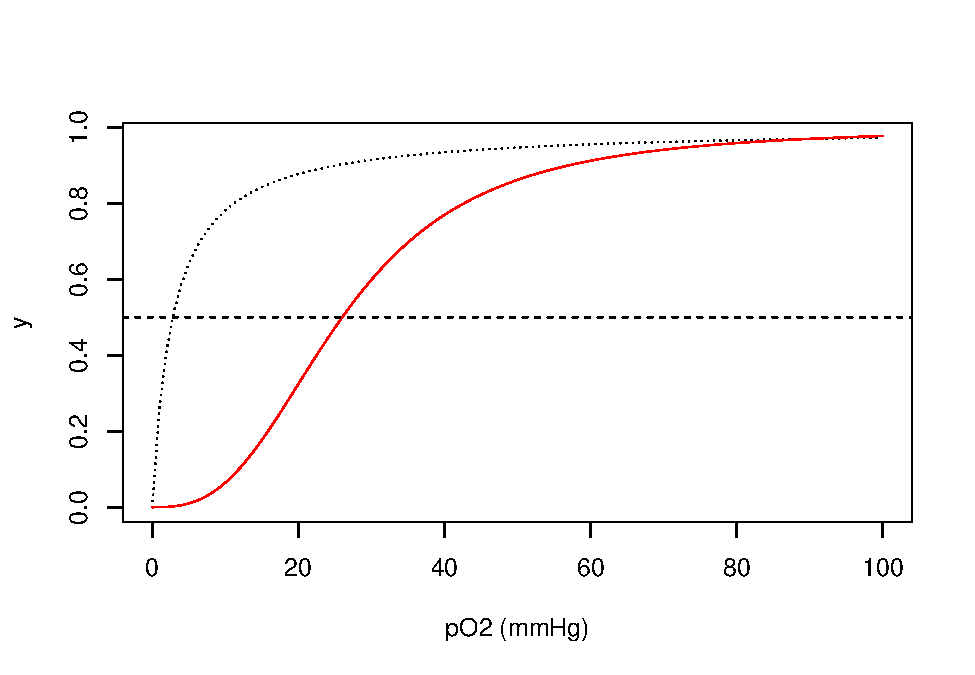
\includegraphics{Bioquímica-Quantitativa-com-R_files/figure-latex/unnamed-chunk-30-1.pdf}
\caption{\label{fig:unnamed-chunk-30}Isoterma de saturação de oxigênio à mioglobina (linha contínua) e hemoglobina (linha pontilhada), indicando o intercepto em pO2 de 50\% (meia saturação).}
\end{figure}

~~~Como mencionado no parágrafo anterior, aos quatro centros de ligação com oxigênio molecular reportam-se quatro constantes microscópicas de equilíbrio de dissociação, de \emph{K1} a \emph{K4}. Simplificando o valor de pO\(_{2}\) para \emph{L}, ligante, é possível também representar a ligação de O\(_{2}\) à hemoglobina pela equação de Adair \citep{pauling1935oxygen}:

\begin{equation}
y=\frac{K1*L+2*K2*K1*L^2+3*K3*K2*K1*L^3+4*K4*K3*K2*K1*L^4} {4*(1+K1*L+2*K2*K1*L^2+3*K3*K2*K1*L^3+4*K4*K3*K2*K1*L^4)}
\label{eq:HbKmicro}
\end{equation}

~~~~Ocorre que existe um efeito estatístico associado à interação em estudo, já que o O\(_{2}\) possui 4 sítios iniciais de interação à hemoglobina \citep{tyuma1973analysis}, valores que reduzem até a saturação dos 4 sítios. Dessa forma, é necessário contabilizar as constantes microscópicas \emph{Ki} em razão desse comprometimento estatístico:

\begin{equation}
Ki_{corr} = \frac{i}{N-1+i}*Ki
\label{eq:HbKStat}
\end{equation}

~~~~No R, isso pode ser auxiliado por um \emph{loop for}:

\begin{lstlisting}[language=R]
K=c(0.011,0.016,0.118,0.400) # vetor de constantes microscópicas de dissociação de Hb para O2
L<-seq(1,201,2) # vetor de teores de O2

Kcorr = c() # inicializa um vetor vazio para saída do vetor corrigido de Ki
N = 4 # declara o número de sítios na Hb
for (i in 1:N) Kcorr[i] = i/(N-i+1)*K[i]
Kcorr # apresenta o vetor de valores de Ki corrigidos para o efeito estatístico
\end{lstlisting}

\begin{lstlisting}
## [1] 0.003 0.011 0.177 1.600
\end{lstlisting}

~~~~Perceba que os valores para \emph{Ki} corrigidos estão em proporção que segue a disponibilidade de sítios, de 4 vezes menor para o 1o. sítio (maior ligação), até 4 vezes maior para o 4o. sítio (menor ligação). Agora é possível aplicar-se a equação \eqref{eq:HbKmicro} utilizando-se as constantes calculadas como segue:

\begin{lstlisting}[language=R]
numer<-K[1]*L+2*K[2]*K[1]*L^2+3*K[3]*K[2]*K[1]*L^3+4*K[4]*K[3]*K[2]*K[1]*L^4
denom<-1+numer
y=numer/denom
plot(L,y,xlab="pO2",type="l",col=2)
\end{lstlisting}

\begin{figure}
\centering
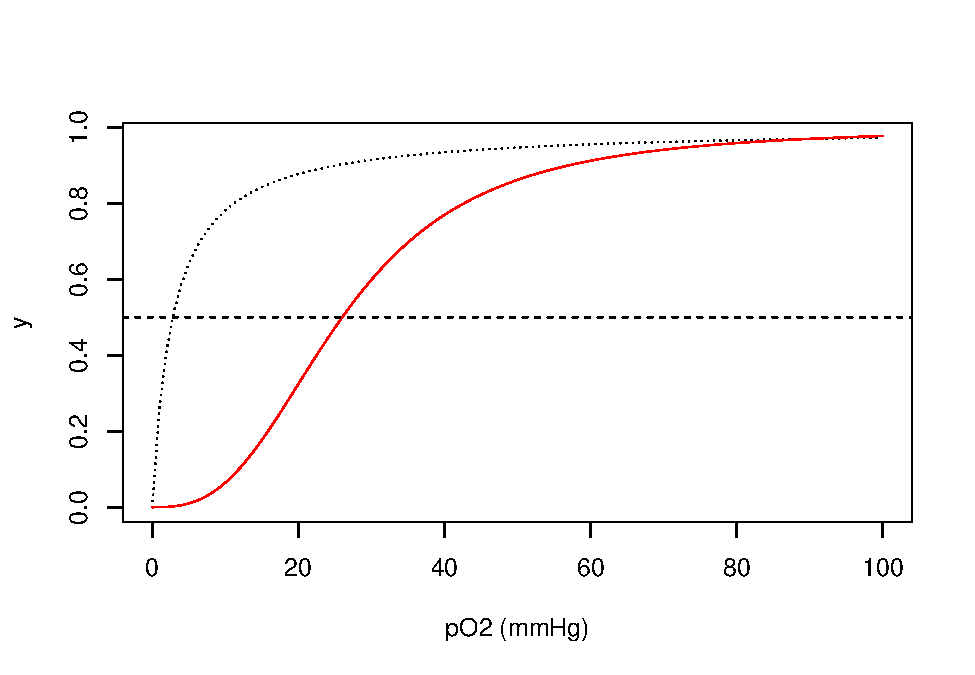
\includegraphics{Bioquímica-Quantitativa-com-R_files/figure-latex/unnamed-chunk-32-1.pdf}
\caption{\label{fig:unnamed-chunk-32}Isoterma de saturação de oxigênio à hemoglobina pela equação de Adair.}
\end{figure}

~~~~~~Por fim, também é possível obter a curva de ligação utilizando-se uma variação de \emph{loop for} na qual a equação \eqref{eq:HbKmicro} é produzida por iteração, como segue \citep{bloomfield2009computer}:

\begin{lstlisting}[language=R]
# Cálculo de y em cada L
  Yi = function(L,Kcorr) {
  N = length(Kcorr)
  conc = c()
  conc[1] = L*Kcorr[1]
  for (i in 2:N) conc[i] = conc[i-1]*L*Kcorr[i]
  numer2 = sum((1:N)*conc)/N
  denom2 = 1 + sum(conc)
  return(numer2/denom2)
}

# Cálculo de y para o vetor de L
    Y = function(L,Kcorr) {
    YY= c()
    for (j in 1:length(L)) YY[j] = Yi(L[j],Kcorr)
    return(YY)
  }

#  Aplicação da função de y para L e gráfico
  Yfinal = Y(L,Kcorr)
  plot(L,Yfinal,type="l", col=2, xlab = "pO2", ylab = "y")
\end{lstlisting}

\begin{figure}
\centering
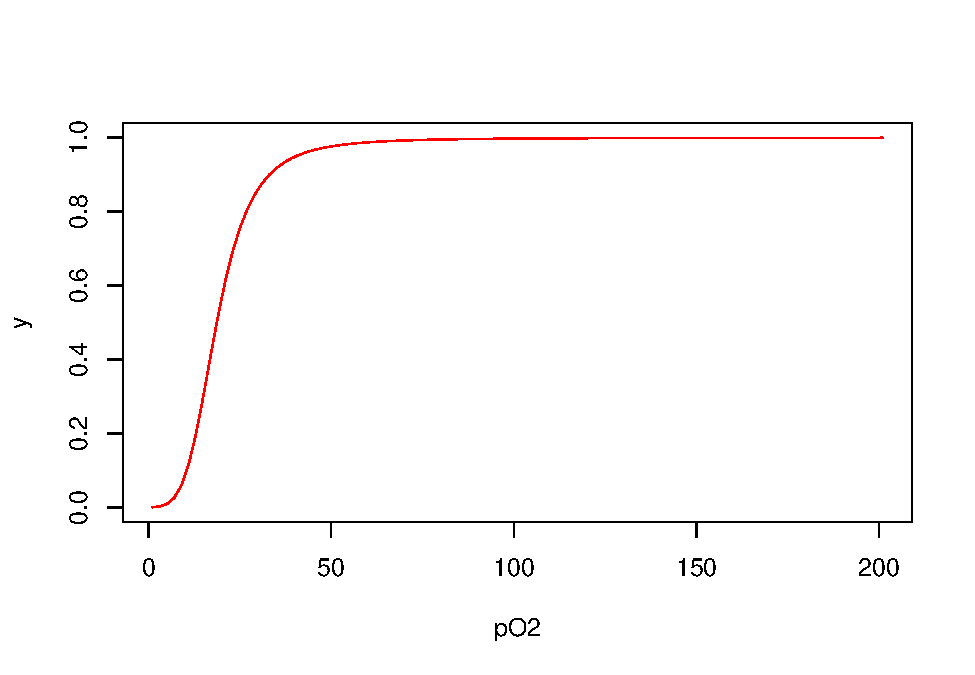
\includegraphics{Bioquímica-Quantitativa-com-R_files/figure-latex/unnamed-chunk-33-1.pdf}
\caption{\label{fig:unnamed-chunk-33}Curva de saturação de oxigênio à hemoglobina obtida por iteração da equação de Adair, tal como corrigida para o efeito estatístico.}
\end{figure}

~~~~~~Observe que há mínimas diferenças entre as curvas obtidas pelos distintos procedimentos, em razão dos diferentes algoritmos utilizados.

\hypertarget{alguns-pacotes-do-r-para-estudo-de-proteuxednas}{%
\section{Alguns pacotes do R para estudo de proteínas}\label{alguns-pacotes-do-r-para-estudo-de-proteuxednas}}

~~~~~~Alguns pacote do R são bastante úteis no estudo de proteínas, em especial a biblioteca \passthrough{\lstinline!seqinr!} vista no capítulo \ref{AAcido}, e que computa diversos valores e informações para sequências proteicas, tais como \emph{pI}, index de hidroxipatia, distribuição de resíduos, entre outros. O sítio do projeto \footnote{Sítio do projeto Seqinr: \url{http://seqinr.r-forge.r-project.org/}} contém informação detalhada para seu uso. Utilizando-se o mesmo procedimento para obtenção da sequência \emph{FASTA} para a lisozima do capítulo \ref{AAcido} (código CAA32175 no sítio \emph{NCBI}), pode-se obter um conjunto extenso de informações da proteína, como exemplificado abaixo:

\begin{lstlisting}[language=R]
library(seqinr)
lisozima<-c("KVFERCELARTLKRLGMDGYRGISLANWMCLAKWESGYNTRATNYNAGDRSTDYGIFQINSRYWCNDGKT
PGAVNACHLSCSALLQDNIADAVACAKRVVRDPQGIRAWVAWRNRCQNRDVRQYVQGCGV")
seq_liso<-s2c(lisozima) # converte sequência de string de aminoácidos para o padrão do seqinr (vetor de caracteres)
seq_liso2<-seq_liso[seq_liso !="\n"] # eliminação de espaços exigida pelo seqinr advindos do procedimento de copiar/colar.
seq_liso2
\end{lstlisting}

\begin{lstlisting}
##   [1] "K" "V" "F" "E" "R" "C" "E" "L" "A" "R" "T" "L" "K" "R" "L" "G" "M" "D"
##  [19] "G" "Y" "R" "G" "I" "S" "L" "A" "N" "W" "M" "C" "L" "A" "K" "W" "E" "S"
##  [37] "G" "Y" "N" "T" "R" "A" "T" "N" "Y" "N" "A" "G" "D" "R" "S" "T" "D" "Y"
##  [55] "G" "I" "F" "Q" "I" "N" "S" "R" "Y" "W" "C" "N" "D" "G" "K" "T" "P" "G"
##  [73] "A" "V" "N" "A" "C" "H" "L" "S" "C" "S" "A" "L" "L" "Q" "D" "N" "I" "A"
##  [91] "D" "A" "V" "A" "C" "A" "K" "R" "V" "V" "R" "D" "P" "Q" "G" "I" "R" "A"
## [109] "W" "V" "A" "W" "R" "N" "R" "C" "Q" "N" "R" "D" "V" "R" "Q" "Y" "V" "Q"
## [127] "G" "C" "G" "V"
\end{lstlisting}

\begin{lstlisting}[language=R]
pmw(seq_liso2) # peso molecular da proteína
\end{lstlisting}

\begin{lstlisting}
## [1] 14701
\end{lstlisting}

\begin{lstlisting}[language=R]
aaa(seq_liso2) # distribuição de resíduos
\end{lstlisting}

\begin{lstlisting}
##   [1] "Lys" "Val" "Phe" "Glu" "Arg" "Cys" "Glu" "Leu" "Ala" "Arg" "Thr" "Leu"
##  [13] "Lys" "Arg" "Leu" "Gly" "Met" "Asp" "Gly" "Tyr" "Arg" "Gly" "Ile" "Ser"
##  [25] "Leu" "Ala" "Asn" "Trp" "Met" "Cys" "Leu" "Ala" "Lys" "Trp" "Glu" "Ser"
##  [37] "Gly" "Tyr" "Asn" "Thr" "Arg" "Ala" "Thr" "Asn" "Tyr" "Asn" "Ala" "Gly"
##  [49] "Asp" "Arg" "Ser" "Thr" "Asp" "Tyr" "Gly" "Ile" "Phe" "Gln" "Ile" "Asn"
##  [61] "Ser" "Arg" "Tyr" "Trp" "Cys" "Asn" "Asp" "Gly" "Lys" "Thr" "Pro" "Gly"
##  [73] "Ala" "Val" "Asn" "Ala" "Cys" "His" "Leu" "Ser" "Cys" "Ser" "Ala" "Leu"
##  [85] "Leu" "Gln" "Asp" "Asn" "Ile" "Ala" "Asp" "Ala" "Val" "Ala" "Cys" "Ala"
##  [97] "Lys" "Arg" "Val" "Val" "Arg" "Asp" "Pro" "Gln" "Gly" "Ile" "Arg" "Ala"
## [109] "Trp" "Val" "Ala" "Trp" "Arg" "Asn" "Arg" "Cys" "Gln" "Asn" "Arg" "Asp"
## [121] "Val" "Arg" "Gln" "Tyr" "Val" "Gln" "Gly" "Cys" "Gly" "Val"
\end{lstlisting}

\begin{lstlisting}[language=R]
AAstat(seq_liso2,plot=TRUE) # gráfico de distribuição, composição e proporção de resíduos, valor de pI 
\end{lstlisting}

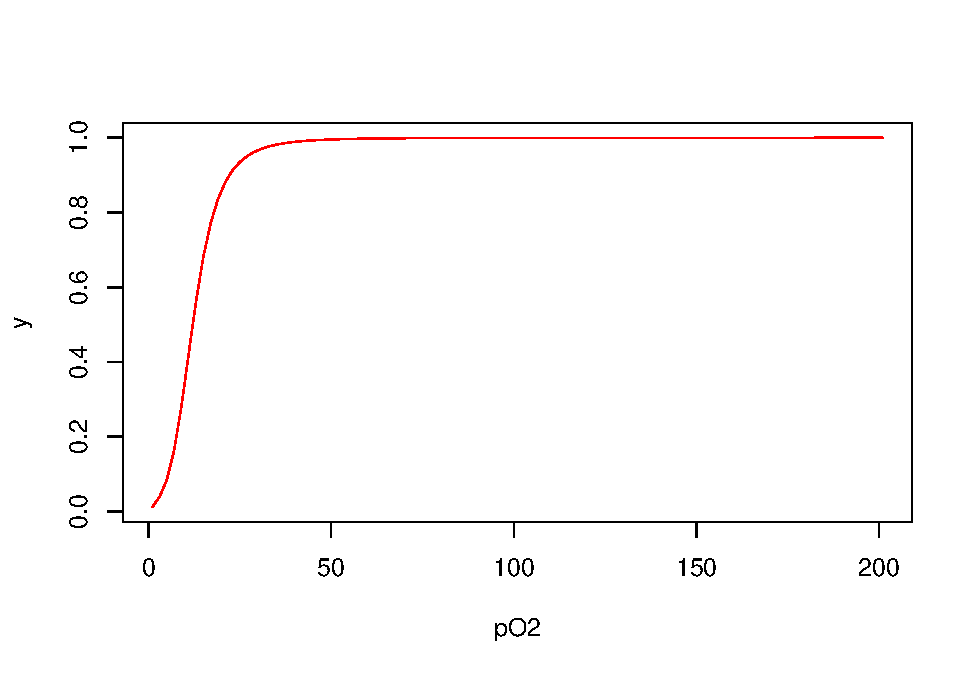
\includegraphics{Bioquímica-Quantitativa-com-R_files/figure-latex/unnamed-chunk-34-1.pdf}

\begin{lstlisting}
## $Compo
## 
##  *  A  C  D  E  F  G  H  I  K  L  M  N  P  Q  R  S  T  V  W  Y 
##  0 14  8  8  3  2 11  1  5  5  8  2 10  2  6 14  6  5  9  5  6 
## 
## $Prop
## $Prop$Tiny
## [1] 0.3
## 
## $Prop$Small
## [1] 0.6
## 
## $Prop$Aliphatic
## [1] 0.2
## 
## $Prop$Aromatic
## [1] 0.1
## 
## $Prop$Non.polar
## [1] 0.6
## 
## $Prop$Polar
## [1] 0.4
## 
## $Prop$Charged
## [1] 0.2
## 
## $Prop$Basic
## [1] 0.2
## 
## $Prop$Acidic
## [1] 0.08
## 
## 
## $Pi
## [1] 9
\end{lstlisting}

~~~~~~Entre outras funções constantes do \passthrough{\lstinline!seqinr!} inclui-se a conversão de aminoácidos para abreviações de 1 e 3 letras (\passthrough{\lstinline!a!}e \passthrough{\lstinline!aaa!}, respectivamente), listagem de 544 propriedades físico-químicas dos 20 aminoácidos proteicos (\passthrough{\lstinline!aaindex!}),\passthrough{\lstinline!pK!} (autoexplicativo, e visto anteriormente), e cômputo isolado de \emph{pI} (\passthrough{\lstinline!computePI!}) e de massa molecular (\passthrough{\lstinline!pmw!}), além de várias outras, tanto para proteômica como para genômica.\\
\hspace*{0.333em}\hspace*{0.333em}\hspace*{0.333em}\hspace*{0.333em}\hspace*{0.333em}\hspace*{0.333em}Outro pacote do R interessante para estudo de proteínas é o \emph{Peptides} \footnote{Pacote Peptides: \url{https://cran.r-project.org/web/packages/Peptides/index.html}}, que também computa diversas propriedades físico-químicas para sequências de aminoácidos, além de possibilitar a integração de plotagem com o pacote de dinâmica molecular \emph{GROMACS}. Como para o \passthrough{\lstinline!seqinr!}, o \passthrough{\lstinline!Peptides!} necessita de conversão da sequência em \emph{string} para o padrão vetorial reconhecido. Entre as funções do pacote destacam-se o cômputo de 66 descritores para cada aminoácido de uma sequência (\passthrough{\lstinline!aaDescriptors!}), a composição da sequência por classificação dos resíduos (\passthrough{\lstinline!aaComp!}), o cômputo de índice alifático (\passthrough{\lstinline!aIndex!}), o índice de hidrofobicidade (\passthrough{\lstinline!hydrophobicity!}), índice de instabilidade (\passthrough{\lstinline!instalIndex!}), relação de massa/carga (\passthrough{\lstinline!mz!}), massa molecular (\passthrough{\lstinline!mw!}), e pI (\passthrough{\lstinline!pI!}), entre outros.\\
\hspace*{0.333em}\hspace*{0.333em}\hspace*{0.333em}\hspace*{0.333em}\hspace*{0.333em}\hspace*{0.333em}Entre pacotes mais direcionados ao estudo comparativo e visualização de estruturas, bem como para descritores de bioinformática e quimiogenômica vale mencionar \passthrough{\lstinline!Bio3d!}, \passthrough{\lstinline!Autoplotprotein!}, \passthrough{\lstinline!protr!}, \passthrough{\lstinline!BioMedR!}, e \passthrough{\lstinline!UniprotR!}, entre muitos.

\hypertarget{Enzimas}{%
\chapter{Enzimas}\label{Enzimas}}

~~~~~~De modo geral, enzimas são estudadas sob diversos pontos de vista, tais como sua estrutura, mecanismo de ação, e comportamento cinético. Este capítulo visa trabalhar nesse último, com auxílio do \passthrough{\lstinline!R!}.\\
\hspace*{0.333em}\hspace*{0.333em}\hspace*{0.333em}\hspace*{0.333em}\hspace*{0.333em}\hspace*{0.333em}De modo geral, a equação simplificada que descreve a atividade de uma enzima \emph{E} sobre um substrato \emph{S} pode ser descrita como:

\begin{equation}
E+S \begin{array}{c}
_{k1}\\
 \rightleftharpoons\\
^{k2} \end{array} ES 
\begin{array}{c}
_{k3}\\
\rightarrow \\
  ^{}\end{array}E+P
 \label{eq:diagMM}
\end{equation}

Onde \emph{P} representa o produto da reação, \emph{ES} o complexo ativado no estado de transição, e \emph{k1}, \emph{k2} e \emph{k3} as constantes de velocidade da reação.

~~~~~~Pela aproximação de Briggs-Haldane para o estado estacionário, e o tratamento de Henri-Michaelis-Menten, a equação que define a curva de velocidade da reação enzimática em função do teor de substrato pode ser descrita abaixo:

\begin{equation}
v=\frac{Vm*S}{Km+S}
\label{eq:eqMM}
\end{equation}

Onde \emph{Km} representa a \emph{constante de Michaelis-Menten}, e \emph{Vm} a velocidade limite da reação (por vezes denominada erroneamente como \emph{velocidade máxima}, embora a hipérbole quadrática descrita pela função não exiba valor máximo por não atingir uma assíntota). Por sua vez \emph{Km} pode ser definido a partir das constantes de velocidade da equação \eqref{eq:diagMM} como:

\begin{equation}
Km=\frac{k1+k3}{k2}
\label{eq:eqMM}
\end{equation}

~~~~~~Portanto, dados os valores de \emph{Vm} e \emph{Km}, podemos descrever um \emph{comportamento de Michaelis-Menten} para uma enzima como:

\begin{lstlisting}[language=R]
Vm= 10
Km = 0.5
curve(Vm*x/(Km+x),xlim=c(0,10),
      xlab="[S]", ylab="v")
abline(h=5,lty=2,col="blue")
abline(v=0.5,lty=2, col="blue")
text(x=1,y=0.2,"Km",col="blue")
text(1,5.3,"Vm/2",col="blue")
\end{lstlisting}

\begin{figure}
\centering
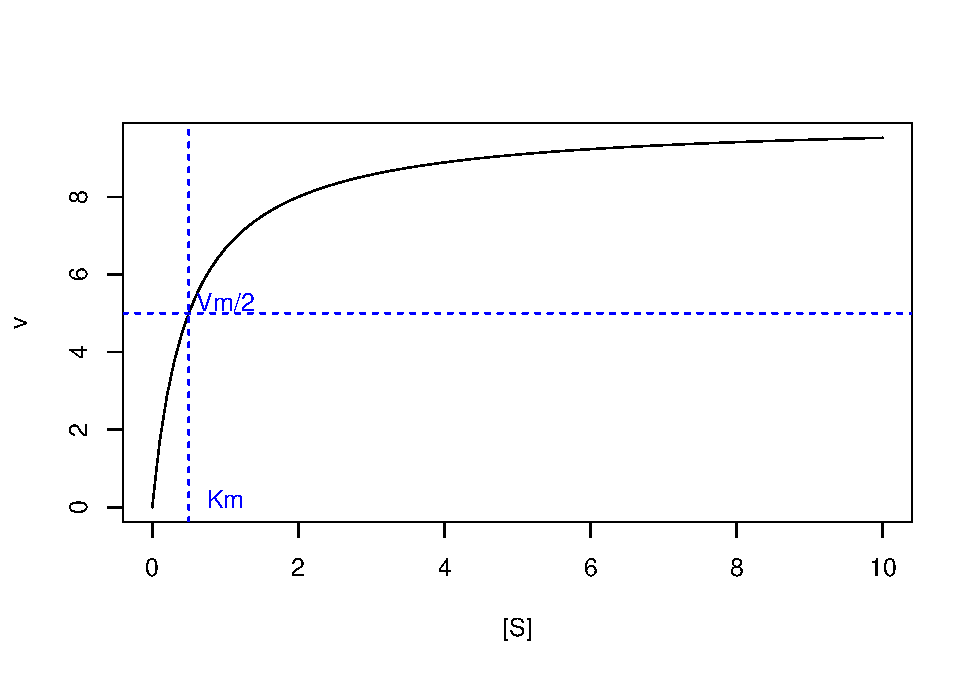
\includegraphics{Bioquímica-Quantitativa-com-R_files/figure-latex/figMM-1.pdf}
\caption{\label{fig:figMM}Curva de Michaelis-Mentem para uma enzima exibindo Vm=10 e Km=0,5 (50 curvas).}
\end{figure}

~~~~~~Por essa relação, o valor de \emph{Km} é representado pelo teor de substrato que confere metade do valor de \emph{Vm} para a reação. Observe que pela equação \eqref{eq:eqMM} o valor de \emph{Km} no denominador influencia inversamente a velocidade \emph{v} da reação; ou seja, quanto maior o valor de \emph{Km}, menor a taxa da reação enzimática. Isto pode ser ilustrado iterativamente com um \emph{loop}, tal como segue:

\begin{lstlisting}[language=R]
Vm=10
Km=seq(from=0.1,to=10,by=0.2) # sequência para 50 valores de Km
for(i in 1:length(Km)) { # loop para adicionar curva de Michaelis-Mentem a cada valor de Km
  add<-if(i == 1) FALSE else TRUE # controle de fluxo que permite adição de curva a partir da segunda iteração (ou seja, quando i > 1)
curve(Vm*x/(Km[i]+x), col= i, lwd=0.8, from =0, to=10, n =100,
      xlab="[S}", ylab="v", add=add)
} 
arrows(0.5,9,3,6,length=0.1,angle=45, col="blue") # seta para Km
text(0.2,9,"Km",col="blue") # indexador para Km
\end{lstlisting}

\begin{figure}
\centering
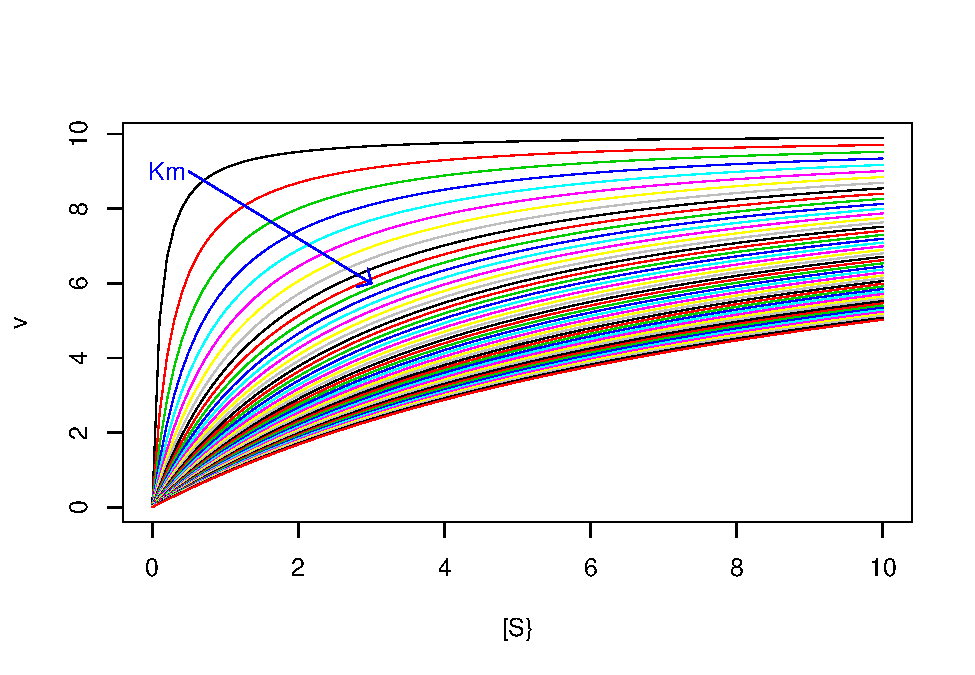
\includegraphics{Bioquímica-Quantitativa-com-R_files/figure-latex/figKm50-1.pdf}
\caption{\label{fig:figKm50}Curvas de Michaelis-Menten com variação iterativa para Km de 0.1 a 10.}
\end{figure}

~~~~~~As curvas representadas nas figuras \ref{fig:figMM} e \ref{fig:figKm50} foram produzidas com a equação \eqref{eq:eqMM}, sendo possível extrair os parâmetros cinéticos \emph{Vm} e \emph{Km} facilmente, já que não há desvios computados para a \emph{velocidade inicial} da reação. Se, por outro lado, estivermos diante de valores experimentais de uma catálise de comportamento de michaelinano e desejarmos extrair os parâmetros cinéticos, melhor será ajustar a equação não-linear de Michaelis-Menten diretamente (algoritmos como Gauss-Newton, Simplex, Levenberg-Marquadt) ou, de modo mais simples, transformar as variáveis \emph{S} e \emph{v} de tal modo que permitam um ajuste linear por mínimos quadrados.\\
\hspace*{0.333em}\hspace*{0.333em}\hspace*{0.333em}\hspace*{0.333em}\hspace*{0.333em}\hspace*{0.333em}Não obstante, a equação que descreve a equação de Michaelis-Mentem constitui uma hipérbole quadrática e, como tal, não possui assíntota matemática, apenas visual. De fato, os próprios autores do trabalho original, Leonor Michaelis e Maud Mentem, reportaram seus dados com a representação de \emph{S} em eixo logaritmo permitindo melhor visualização da região assintótica do gráfico \citep{michaelisment1913}.

\hypertarget{obtenuxe7uxe3o-de-paruxe2metros-cinuxe9ticos-a-partir-de-dados-expermentais-simulados}{%
\section{Obtenção de parâmetros cinéticos a partir de dados expermentais simulados}\label{obtenuxe7uxe3o-de-paruxe2metros-cinuxe9ticos-a-partir-de-dados-expermentais-simulados}}

~~~~~~Para a determinação dos parâmetros cinéticos \emph{Vm} e \emph{Km} obtidos a partir de uma simulação experimental de dados de \emph{S} e \emph{v}, é necessário em primeiro lugar obter-se os pontos experimentais, tal como segue:

\begin{lstlisting}[language=R]
Vm=10
Km=0.5
set.seed(1500) # fixa a semente para geração de dados aleatórios reproduzíveis
erro=runif(20,0,1) # comando para erro uniforme (no. de pontos, min, max)
curve(Vm*x/(Km+x)+erro, type="p", from =0, to=1, n =20,
      xlab="[S}", ylab="v") # elaboração da curva com cômputo de erro uniforme
\end{lstlisting}

\begin{figure}
\centering
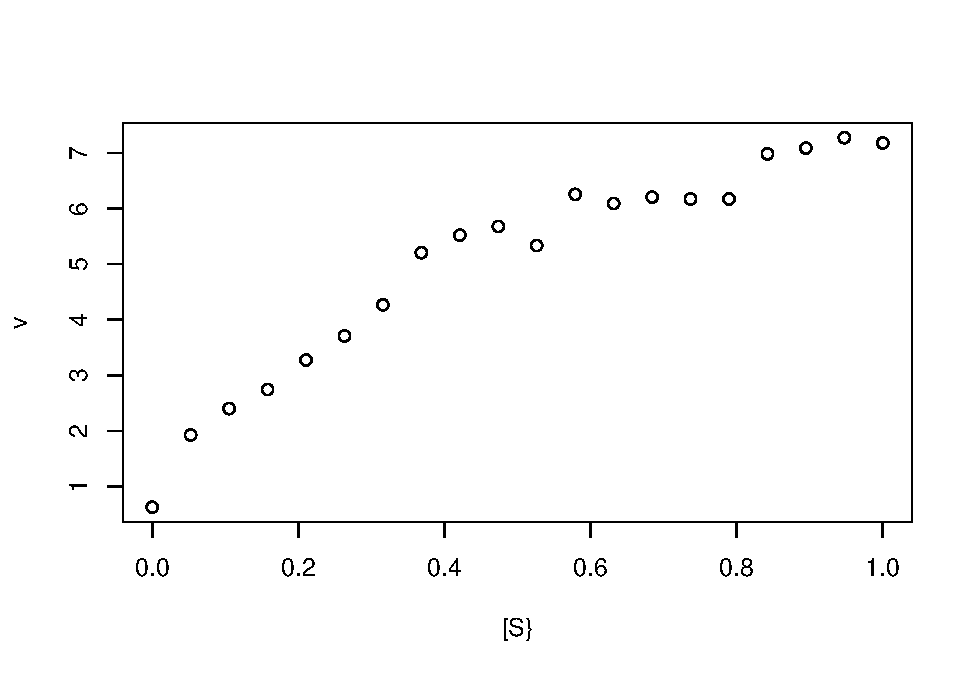
\includegraphics{Bioquímica-Quantitativa-com-R_files/figure-latex/simulMM-1.pdf}
\caption{\label{fig:simulMM}Simulação de pontos experimentais (n=20) obtidos a partir da equação de Michaelis-Menten.}
\end{figure}

~~~~~~Perceba que pela figura \ref{fig:simulMM}, já não é mais possível definir-se uma região assintótica que permita a determinação de \emph{Vm} e, por consequência, de \emph{Km}. Nesse caso, pode-se obter os parâmetros cinéticos por tranformação da função hiperbólica de Michaelis-Mentem para uma função linear correlata, sucedendo-se o ajuste linear dos dados transformados para a obtenção dos parâmetros de catálise.

\hypertarget{linearizauxe7uxf5es-e-ajustes}{%
\section{Linearizações e ajustes}\label{linearizauxe7uxf5es-e-ajustes}}

~~~~~~Diversas são as linearizações encontradas na literatura para a equação de Michaelis-Mentem. Para exemplificá-las, segue um trecho de código contendo as quatro mais empregadas. Para isso utilizou-se um par de funções do \passthrough{\lstinline!R!} para, respectivamente, estabelecer a área gráfica e sua subdivisão para plotagem em 4 paineis (\passthrough{\lstinline!par!} e \passthrough{\lstinline!mfrow!} ou \passthrough{\lstinline!mfcol!}):

\begin{lstlisting}[language=R]
S=c(0.1,0.2,0.5,1,5,10,20) # cria um vetor para substrato
Km=0.5;Vm=10 # estabelece os parâmetros enzimáticos
v=Vm*S/(Km+S) # aplica a equação de MM ao vetor de S
par(mfrow=c(2,2)) # estabelece área de plot pra 4 gráficos
plot(S,v,type="o",main="Michaelis-Mentem")
plot(1/S,1/v,type="o",main="Lineweaver-Burk")
plot(v,v/S,type="o",main="Eadie-Hofstee")
plot(S,S/v,type="o",main="Hanes-Woolf")
\end{lstlisting}

\begin{figure}
\centering
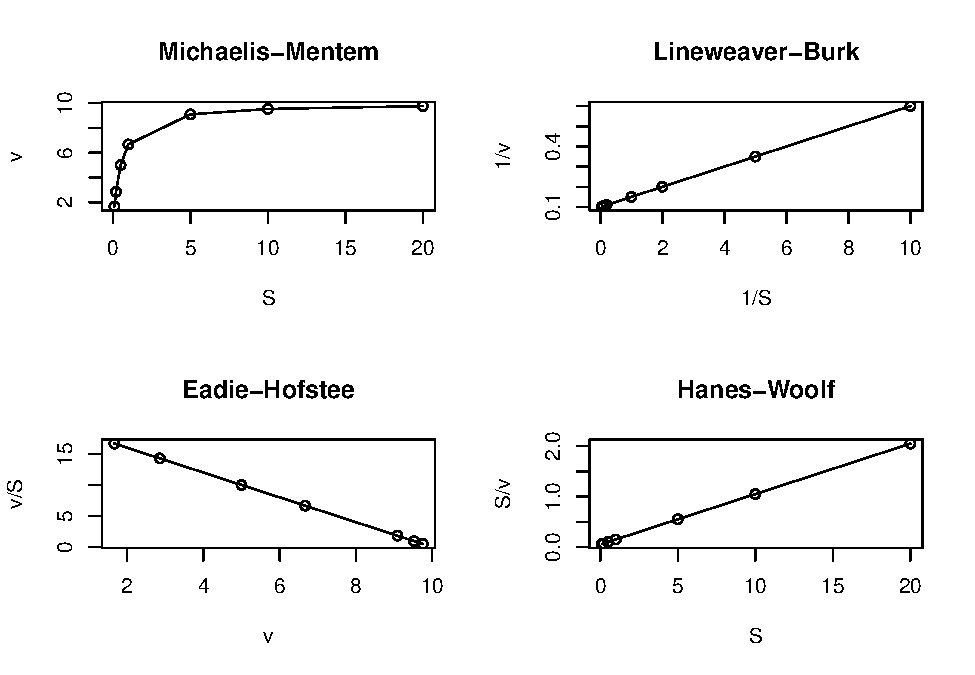
\includegraphics{Bioquímica-Quantitativa-com-R_files/figure-latex/figLin-1.pdf}
\caption{\label{fig:figLin}Principais linearizações da equação de Michaelis-Menten.}
\end{figure}

\begin{lstlisting}[language=R]
layout(1) # volta à janela gráfica normal
\end{lstlisting}

~~~~~~Dentre essas transformações lineares para cinética enzimática, as mais frequentemente encontradas são de \emph{Lineweaver-Burk} (ou duplo-recíproco), e a de \emph{Eadie-Hofstee}, sendo a primeira a mais comum na literatura. No entanto, a aplicação do formalismo de Eadie-Hofstee para interação ligante-proteína também é a mais reportada nessa área, embora seja tratada como representação de Scatchard \citep{scatchard1949attractions}.

\hypertarget{linearizauxe7uxe3o-por-transformauxe7uxe3o-de-lineweaver-burk}{%
\subsection{Linearização por transformação de Lineweaver-Burk}\label{linearizauxe7uxe3o-por-transformauxe7uxe3o-de-lineweaver-burk}}

~~~~~~A forma linear para a equação de Linewaver-Burk é obtida a partir da transformação da equação de Michaelis-Menten que segue:

\begin{equation}
\frac{1}{v}=\frac{1}{Vm}+\frac{Km}{Vm}*\frac{1}{S}
\label{eq:eqLB}
\end{equation}

~~~~~~Dessa forma, os dados obtidos pela figura \ref{fig:simulMM} são transformados para seu duplo-recíproco, resultando em:

\begin{lstlisting}[language=R]
S=seq(0.1,1,length.out=20) # gera uma sequência com 20 pontos entre 0 e 1 para valores de substrato
Vm=10; Km=0.5 # parâmetros cinéticos
set.seed(1500) # estabelecer a mesma semente aleatória do gráfico direto de Michaelis-Menten, para reproducibilidade dos pontos
erro=runif(20,0,1) # comando para erro uniforme (no. de pontos, min, max)
v=Vm*S/(Km+S)+erro # equação de Michaelis-Menten

inv.S=1/S # cria variáveis para o duplo-recíproco
inv.v=1/v
plot(inv.v~inv.S, xlab="1/S", ylab="1/v") # elabora o gráfico de Lineweaver-Burk
\end{lstlisting}

\begin{figure}
\centering
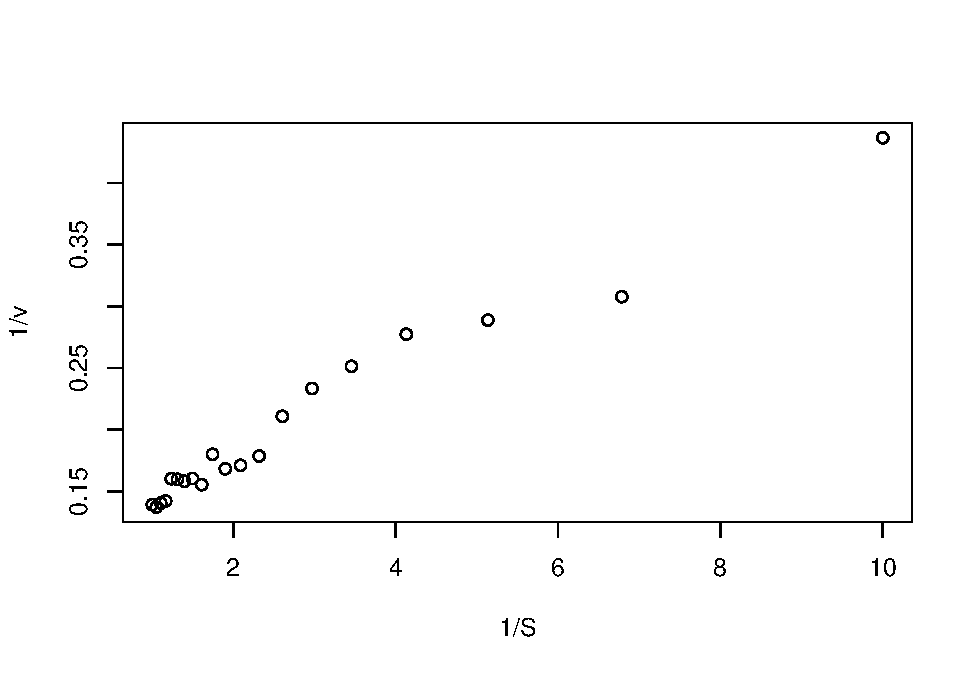
\includegraphics{Bioquímica-Quantitativa-com-R_files/figure-latex/figLB-1.pdf}
\caption{\label{fig:figLB}Representação de Lineweaver-Burk para os dados simulados da curva de Michaelis-Menten.}
\end{figure}

~~~~~~Observe que a figura \ref{fig:figLB} apresenta agora um uma distribuição de valores que possibilita seu ajuste linear por mínimos quadrados (regressão linear). No \passthrough{\lstinline!R!}, isso pode ser facilmente conduzido pelo trecho de código (\emph{chunk}) que segue:

\begin{lstlisting}[language=R]
reg.LB<-lm(inv.v~inv.S) # expressão para ajuste linear
summary(reg.LB) # resultados do ajuste
\end{lstlisting}

\begin{lstlisting}
## 
## Call:
## lm(formula = inv.v ~ inv.S)
## 
## Residuals:
##      Min       1Q   Median       3Q      Max 
## -0.02820 -0.00986 -0.00350  0.00748  0.02842 
## 
## Coefficients:
##             Estimate Std. Error t value Pr(>|t|)    
## (Intercept)  0.11363    0.00515    22.1  1.7e-14 ***
## inv.S        0.03277    0.00146    22.4  1.3e-14 ***
## ---
## Signif. codes:  0 '***' 0.001 '**' 0.01 '*' 0.05 '.' 0.1 ' ' 1
## 
## Residual standard error: 0.01 on 18 degrees of freedom
## Multiple R-squared:  0.965,  Adjusted R-squared:  0.964 
## F-statistic:  503 on 1 and 18 DF,  p-value: 1.33e-14
\end{lstlisting}

\begin{lstlisting}[language=R]
plot(inv.v~inv.S, xlab="1/S", ylab="1/v") # gráfico de Lineweaver-Burk
abline(reg.LB, col="blue") # sobreposição do ajuste ao gráfico
\end{lstlisting}

\begin{figure}
\centering
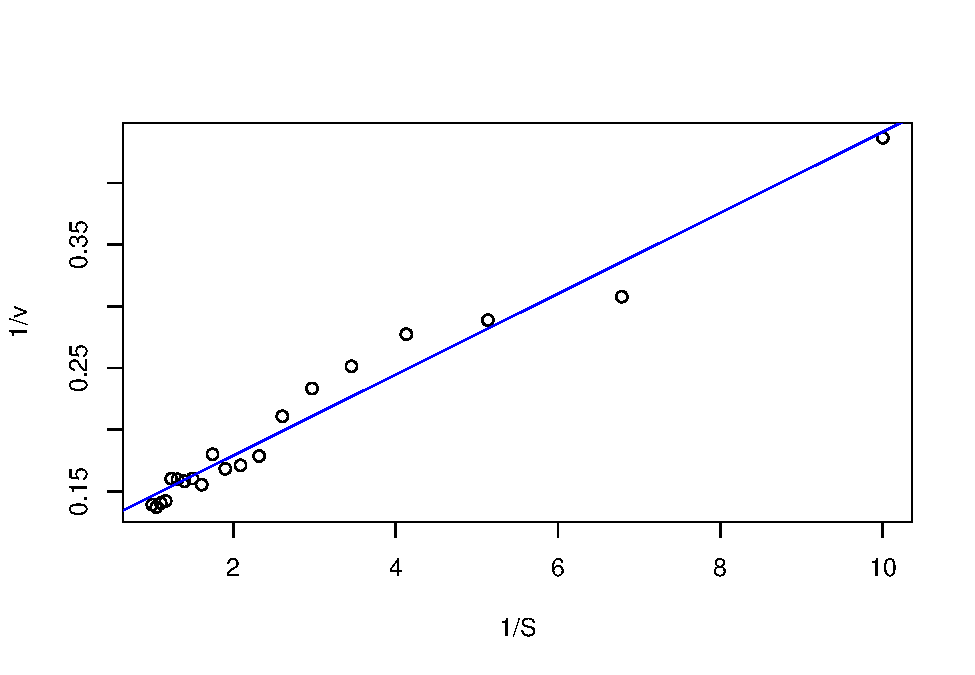
\includegraphics{Bioquímica-Quantitativa-com-R_files/figure-latex/figLBlin-1.pdf}
\caption{\label{fig:figLBlin}Ajuste linear para os dados de Lineweaver-Burk.}
\end{figure}

~~~~~~A tabela produzida pelo \passthrough{\lstinline!R!} para a função \passthrough{\lstinline!lm!} de ajuste linear por mínimos quadrados possui diversas informações que nos permite avaliar a qualidade da regressão. Brevemente, esse tabela nos fornece o valor de cada parâmetro do ajuste conforme a equação que segue:

\begin{equation}
y = a + b *x
\label{eq:eqLin}
\end{equation}

~~~~~~Nesse caso, \emph{a} refere-se ao intercepto presente na tabela (\emph{(intercept)}, ou 1/Vm) e \emph{b} à inclinação (\emph{inv.S}, ou Km/Vm). Além disso, a tabela também fornece diversos resultados complentares, elencados a seguir:

\begin{enumerate}
\def\labelenumi{\arabic{enumi}.}
\item
  valor de erro-padrão dos parâmetros (\emph{Std. Error});
\item
  valor da distribuição \emph{t} de Student (\emph{t value});
\item
  o respectivo nível de probabilidade (\emph{Pr}) com indicação de significância (asteriscos);
\item
  erro padrão residual (\emph{Residual standard error});
\item
  valor dos coeficientes de determinação bruto (\emph{Multiple R-squared}) e ajustado para os graus de liberdade (\emph{Adjusted R-squared});
\item
  valor da distribuição F de Snedocor (\emph{F-statistic}) de variância do ajuste;
\item
  graus de liberdade (\emph{DF}) e o valor de significância da regressão ao modelo linear obtido pela análise de variância (\emph{p-value}).
\end{enumerate}

~~~~~~Não obstante, a qualidade do ajuste linear também pode ser verificada pela produção de gráficos diagnósticos estatísticos, bastando-se aplicar o trecho simples abaixo:

\begin{lstlisting}[language=R]
plot(reg.LB) # comando para geração de gráficos diagnósticos de ajuste linear
\end{lstlisting}

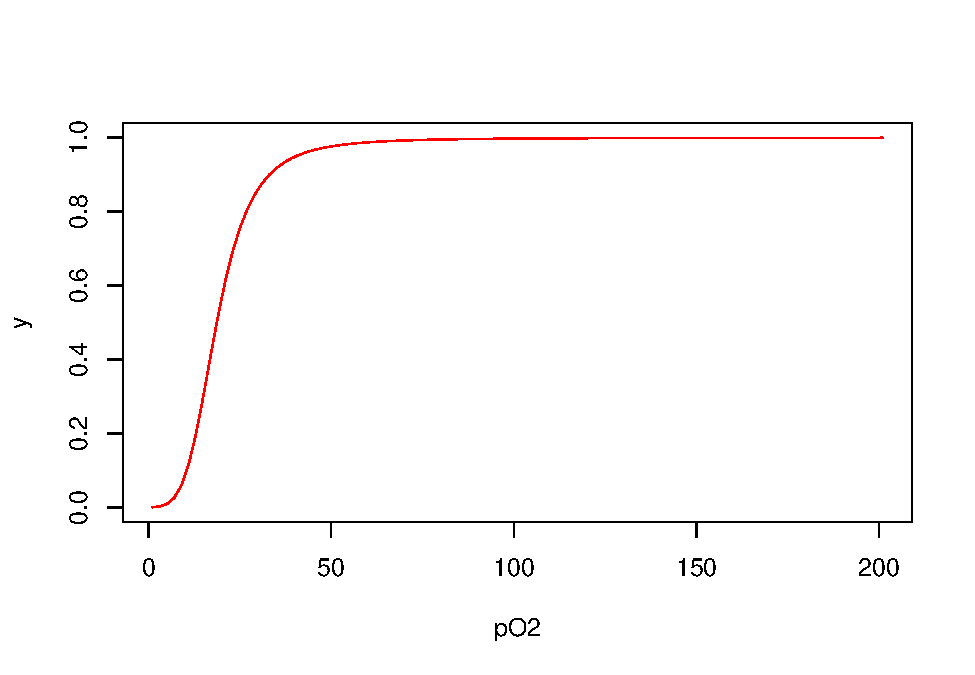
\includegraphics{Bioquímica-Quantitativa-com-R_files/figure-latex/unnamed-chunk-35-1.pdf} 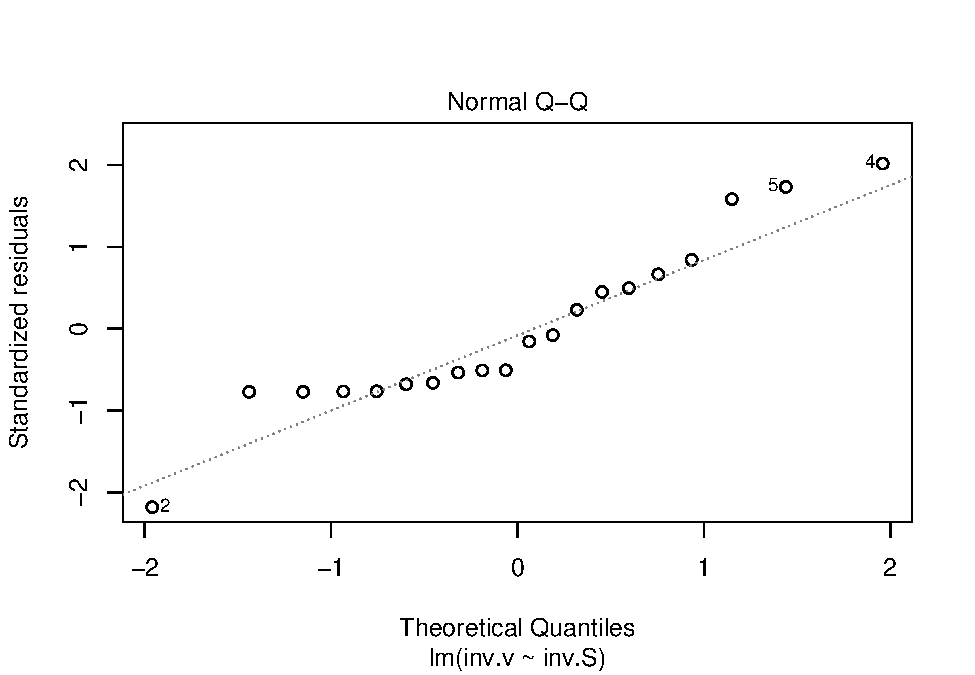
\includegraphics{Bioquímica-Quantitativa-com-R_files/figure-latex/unnamed-chunk-35-2.pdf} 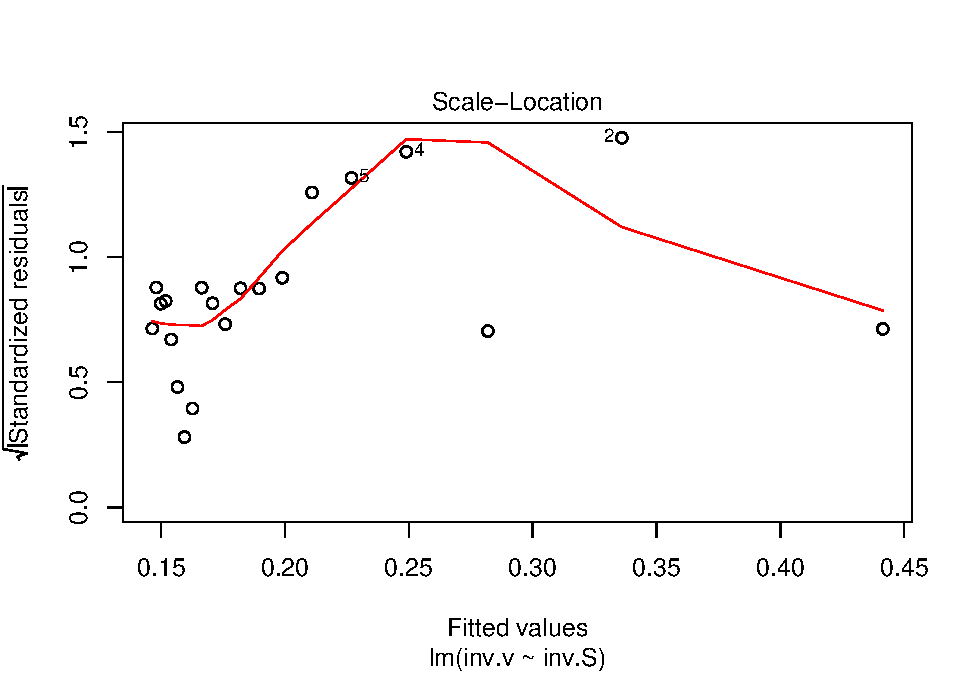
\includegraphics{Bioquímica-Quantitativa-com-R_files/figure-latex/unnamed-chunk-35-3.pdf} 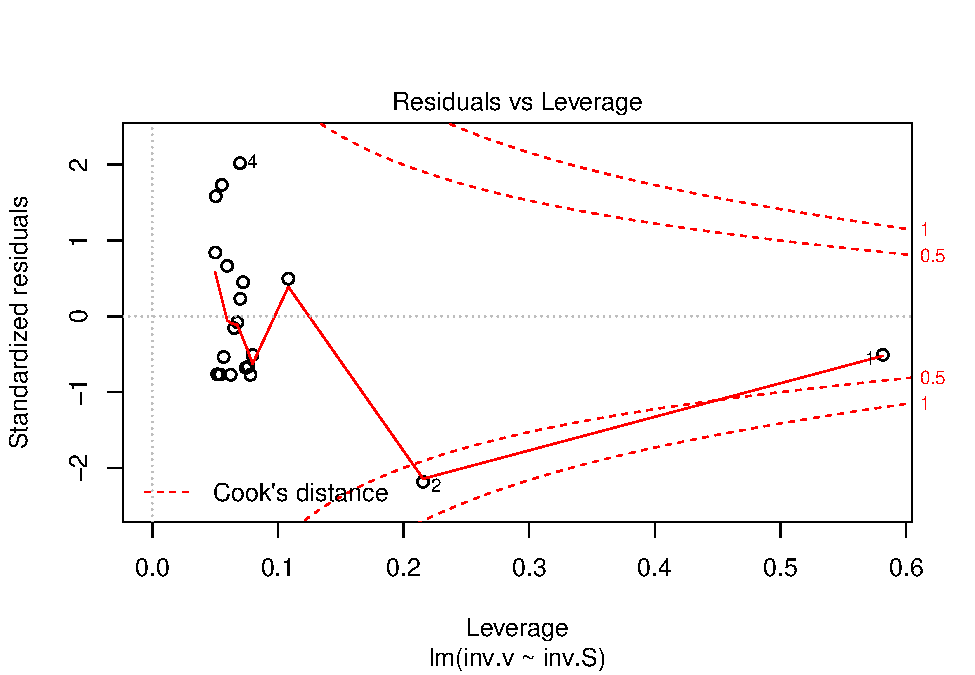
\includegraphics{Bioquímica-Quantitativa-com-R_files/figure-latex/unnamed-chunk-35-4.pdf}

~~~~~~Esses gráficos diagnósticos também podem ser alocados em paineis, como ilustrado para as linearizações de Michaelis-Mentem acima.

\begin{lstlisting}[language=R]
reg.LB<-lm(inv.v~inv.S)
par(mfrow = c(2, 2))
plot(reg.LB)
\end{lstlisting}

\begin{figure}
\centering
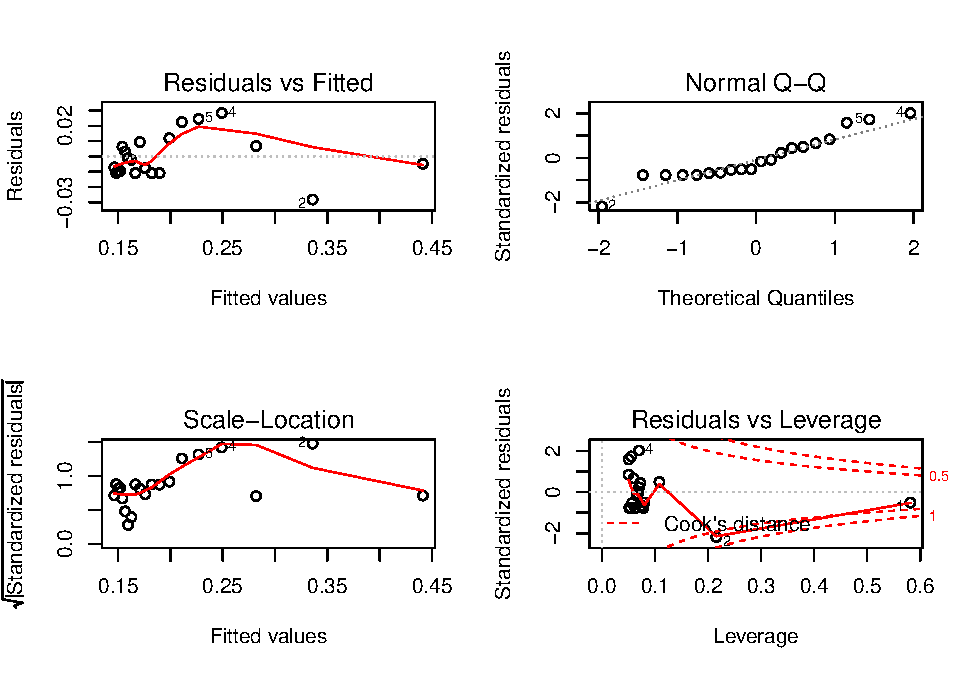
\includegraphics{Bioquímica-Quantitativa-com-R_files/figure-latex/figLinDiag-1.pdf}
\caption{\label{fig:figLinDiag}Gráficos diagnósticos de ajuste linear.}
\end{figure}

\begin{lstlisting}[language=R]
layout(1)
\end{lstlisting}

~~~~~~Os quatro gráficos gerados acima referem-se, respectivamente, 1) à variação de resíduos com os valores ajustados, 2) a um teste de distribuição normal dos resíduos, 3) à variação de resíduos padronizados em função dos valores ajustados, e 4) à observação de valores influenciáveis identificáveis pela \emph{distância de Cook} para cada observação. Em relação à esse último, pode-se opcionalmente definir sua aparência para identificação daqueles valores por seleção (\passthrough{\lstinline!which!}, 4 ou 6, por ex), tal como em:

\begin{lstlisting}[language=R]
plot(reg.LB, which = 4)
\end{lstlisting}

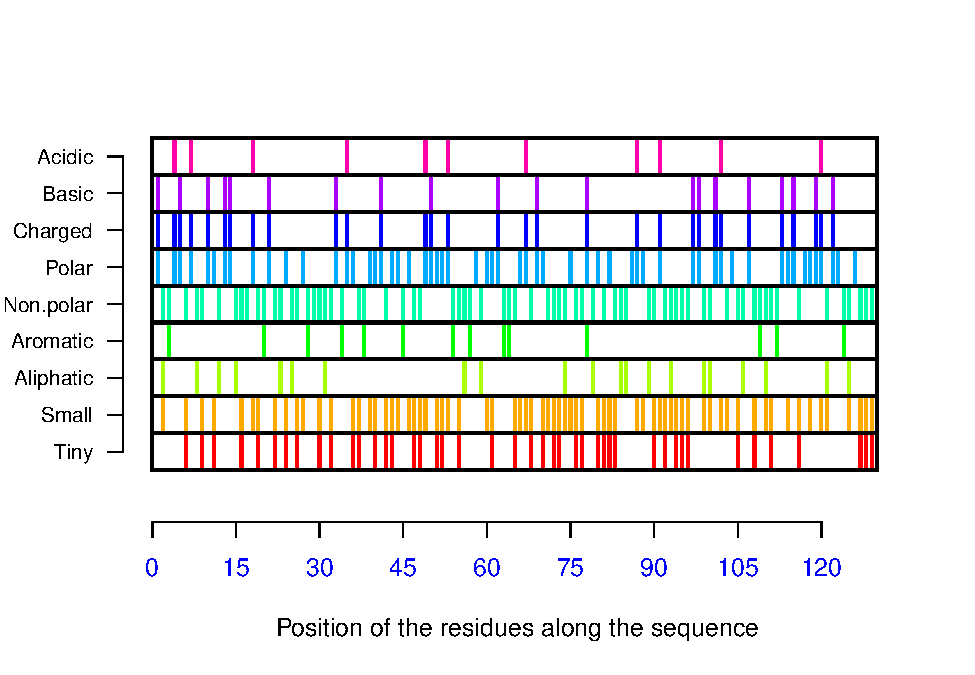
\includegraphics{Bioquímica-Quantitativa-com-R_files/figure-latex/unnamed-chunk-36-1.pdf}

~~~~~~Por esses dois procedimentos, tabela e gráficos diagnósticos, é possível aferir a qualidade de um ajuste linear pelo \passthrough{\lstinline!R!}. Em paralelo, diversas são as funções associadas à própria função \passthrough{\lstinline!lm!} para modelos lineares (objetos), o que reforça o caráter de linguagem orientada a objeto do \passthrough{\lstinline!R!}. Entre essas vale citar, com significado intuitivo, \passthrough{\lstinline!coef!}, \passthrough{\lstinline!fitted!}, \passthrough{\lstinline!predict!}, \passthrough{\lstinline!residuals!}, \passthrough{\lstinline!confint!}, e \passthrough{\lstinline!deviance!}.\\
\hspace*{0.333em}\hspace*{0.333em}\hspace*{0.333em}\hspace*{0.333em}\hspace*{0.333em}\hspace*{0.333em}Para acessar os parâmetros contidos na função \passthrough{\lstinline!lm!}, assim como outras de mesma natureza no \passthrough{\lstinline!R!}, basta digitar \passthrough{\lstinline!args!}:

\begin{lstlisting}[language=R]
args(lm)
\end{lstlisting}

\begin{lstlisting}
## function (formula, data, subset, weights, na.action, method = "qr", 
##     model = TRUE, x = FALSE, y = FALSE, qr = TRUE, singular.ok = TRUE, 
##     contrasts = NULL, offset, ...) 
## NULL
\end{lstlisting}

~~~~~~Complementarmente, vale mencionar a existência de inúmeros pacotes do \passthrough{\lstinline!R!} para diversas situações e tratamentos estatísticos de dados para modelos lineares, e que fogem ao escopo deste manuscrito, tais como os que possibilitam análises de \emph{outliers} (valores extremos), \emph{Generalized Linear Models}, \emph{Mixed Effects Models}, \emph{Non-parametric Regression}, entre outros. Entre os pacotes do \passthrough{\lstinline!R!} complementares para regressão linear vale mencionar \passthrough{\lstinline!car!}, \passthrough{\lstinline!MASS!}, \passthrough{\lstinline!caret!}, \passthrough{\lstinline!glmnet!}, \passthrough{\lstinline!sgd!}, \passthrough{\lstinline!BLR!}, e \passthrough{\lstinline!Lars!}.

\hypertarget{considerauxe7uxf5es-sobre-a-linearizauxe7uxe3o-por-lineweaver-burk.}{%
\subsubsection{Considerações sobre a linearização por Lineweaver-Burk.}\label{considerauxe7uxf5es-sobre-a-linearizauxe7uxe3o-por-lineweaver-burk.}}

~~~~~~De volta ao estudo da cinética de estado estacionário da catálise enzimática, mencionamos acima a possibilidade de linearizações da equação de Michaelis-Mentem por dois tratamentos mais comuns, Lineweaver-Burk e Eadie-Hofstee. De modo geral, qualquer tratamento que resulte na transformação de um modelo original (equação de Michaelis-Menten, no caso) por linearização resultará em desvios estatísticos.

~~~~~~Analisando a equação de Lineweaver-Burk, por exemplo, pode-se evidenciar que, como os valores de \emph{S} e \emph{v} estão representados por seus recíprocos, uma pequena variação em \emph{v} resultará numa grande variação em \emph{1/v}. Por outro lado, a escolha da faixa de teores de \emph{S} também é extremamente importante para a extração de parâmetros cinéticos. Isso pode ser ilustrado no exemplo que segue:

\begin{lstlisting}[language=R]
Vm=10; Km=0.5
set.seed(1500) # semente fixa para erro aleatório
erro=runif(length(S),0,0.1)
S=seq(1,10,0.1)
v=Vm*S/(Km+S)+erro
\end{lstlisting}

\begin{lstlisting}
## Warning in Vm * S/(Km + S) + erro: longer object length is not a multiple of
## shorter object length
\end{lstlisting}

\begin{lstlisting}[language=R]
plot(v~S, xlab="S", ylab="v")
\end{lstlisting}

\begin{figure}
\centering
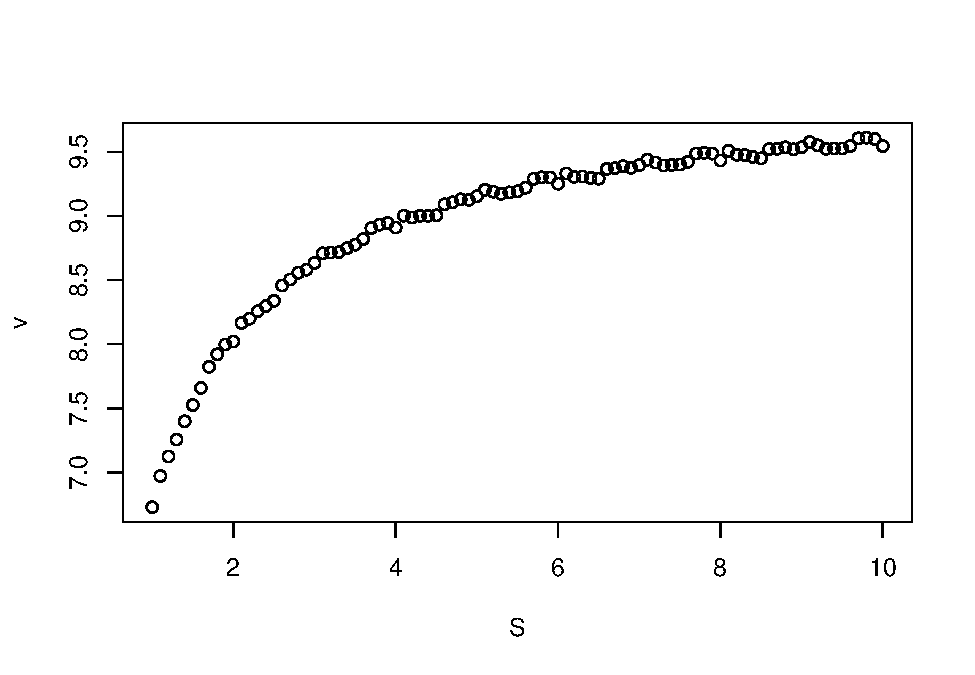
\includegraphics{Bioquímica-Quantitativa-com-R_files/figure-latex/figMM2-1.pdf}
\caption{\label{fig:figMM2}Curva de Michaelis-Mentem simulada com erro experimental aleatório. Vm=10; Km=0.5.}
\end{figure}

~~~~~~Observe que a figura \ref{fig:figMM2} inicia em velocidade próxima a zero, e termina em velocidade próxima à \emph{Vm}, com teor de \emph{S \textgreater\textgreater{} Km} (50 vezes, de fato). Essa condição permite uma extração segura dos parâmetros cinéticos, os quais podem ser obtidos a partir do ajuste linear do gráfico duplo-recíproco.

\begin{lstlisting}[language=R]
set.seed(1500) # semente fixa para erro aleatório
erro=runif(length(S),0,0.2)
Vm=10; Km=0.5 # parâmetros cinéticos
inv.S=1/seq(1,10,0.1) # 1/S
inv.v=1/(Vm*S/(Km+S)+erro) # 1/v
plot(inv.S,inv.v)
lm.LB2<-lm(inv.v~inv.S) # ajuste linear
summary(lm.LB2) #resultados do ajuste
\end{lstlisting}

\begin{lstlisting}
## 
## Call:
## lm(formula = inv.v ~ inv.S)
## 
## Residuals:
##       Min        1Q    Median        3Q       Max 
## -0.001505 -0.000561 -0.000146  0.000752  0.001412 
## 
## Coefficients:
##             Estimate Std. Error t value Pr(>|t|)    
## (Intercept) 0.099181   0.000136     731   <2e-16 ***
## inv.S       0.048156   0.000419     115   <2e-16 ***
## ---
## Signif. codes:  0 '***' 0.001 '**' 0.01 '*' 0.05 '.' 0.1 ' ' 1
## 
## Residual standard error: 8e-04 on 89 degrees of freedom
## Multiple R-squared:  0.993,  Adjusted R-squared:  0.993 
## F-statistic: 1.32e+04 on 1 and 89 DF,  p-value: <2e-16
\end{lstlisting}

\begin{lstlisting}[language=R]
abline(lm.LB2, col="blue")
\end{lstlisting}

\begin{figure}
\centering
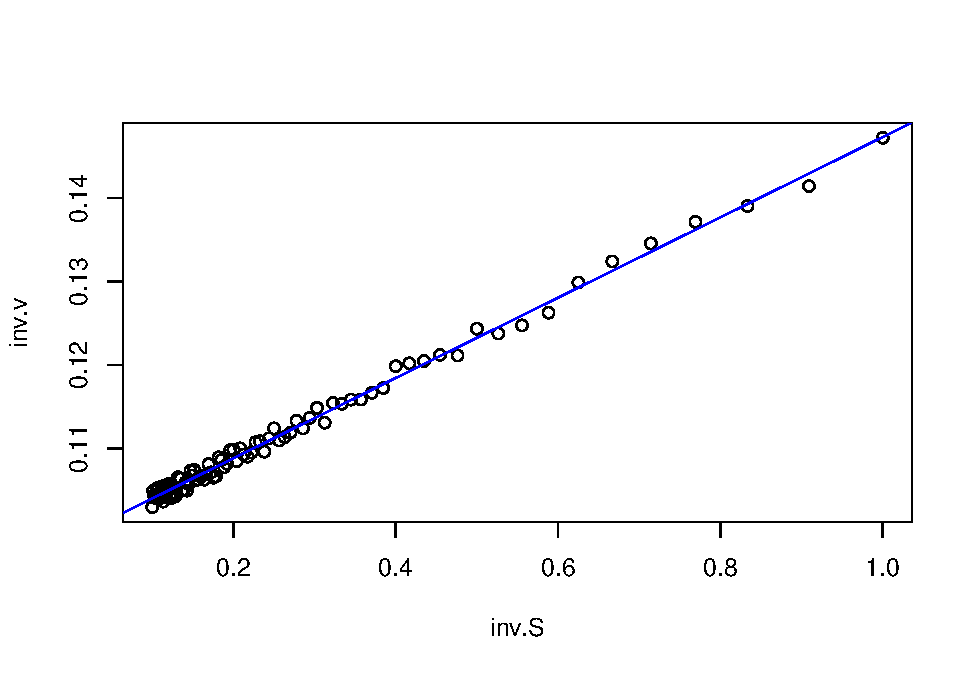
\includegraphics{Bioquímica-Quantitativa-com-R_files/figure-latex/figLB2-1.pdf}
\caption{\label{fig:figLB2}Lineweaver-Burk dos dados do gráfico anterior.}
\end{figure}

~~~~~~Perceba como os valores de \emph{Vm} e \emph{Km} ajustados aproximaram-se dos valores preditos, já que para o gráfico duplo-recíproco:

\begin{equation}
Vm=1/intercepto
\\
Km = intercepto * Vm
\label{eq:eqParLB}
\end{equation}

~~~~~~Agora, o que aconteceria se os pontos experimentais estivessem em faixas distintas de teores de \emph{S} ? Exemplificando, se os pontos fossem coletados em três regiões distintas de \emph{S}: 10-100, 30-100, e 50-100 ?

Isso pode ser ilustrado variando-se a faixa de valores de \emph{S} iterativamente, e inspecionando-se o gráfico duplo-recíproco resultante como no trecho de código que segue, e para os mesmos valores da figura \ref{fig:figLB2}.

\begin{lstlisting}[language=R]
set.seed(1500) # mesma semente aleatória para reproducibilidade de erro
Vm=10; Km=0.5 # estabelece os parâmetros de MM
S=seq(10,100,10) # cria-se uma sequência inicial para S
v=Vm*S/(Km+S) # aplicação equação de MM à S
plot(1/S,1/v, type="n",ylim=c(0.098,0.106)) # elabora o duplo-recíproco sem pontos
 for(i in 1:3) { # inicia a iteração para gráficos de Lineweaver-Burk
   S=seq(10*i,100,length.out=100) # gera uma sequência S com 100 pontos, produzindo 5 vetores que iniciam em valores diferentes para S (10, 30 e 50)
   erro=runif(length(S),0,0.1) #  erro para adição à vetor de velocidade inicial, com no. de pontos em função do vetor de S
    add<-if(i == 1) FALSE else TRUE # controle de fluxo para plotagem de pontos no gráfico vazio
    inv.S=1/S; inv.v=1/((Vm*S/(Km+S))+erro)  # novos valores para o duplo-recíproco em função da iteração
 points(inv.v~inv.S, xlab="1/S", ylab="1/v", col=i, add=add) # adição de pontos ao gráfico de Lineweaver-Burk, com identificação por cores (1, 2, 3, 4 e 5)
 lm.LB<-lm(inv.v~inv.S) # elabora o ajuste linear
 abline(lm.LB, col=i, lty=i) # sobrepõe as linhas de ajuste
 }
\end{lstlisting}

\begin{figure}
\centering
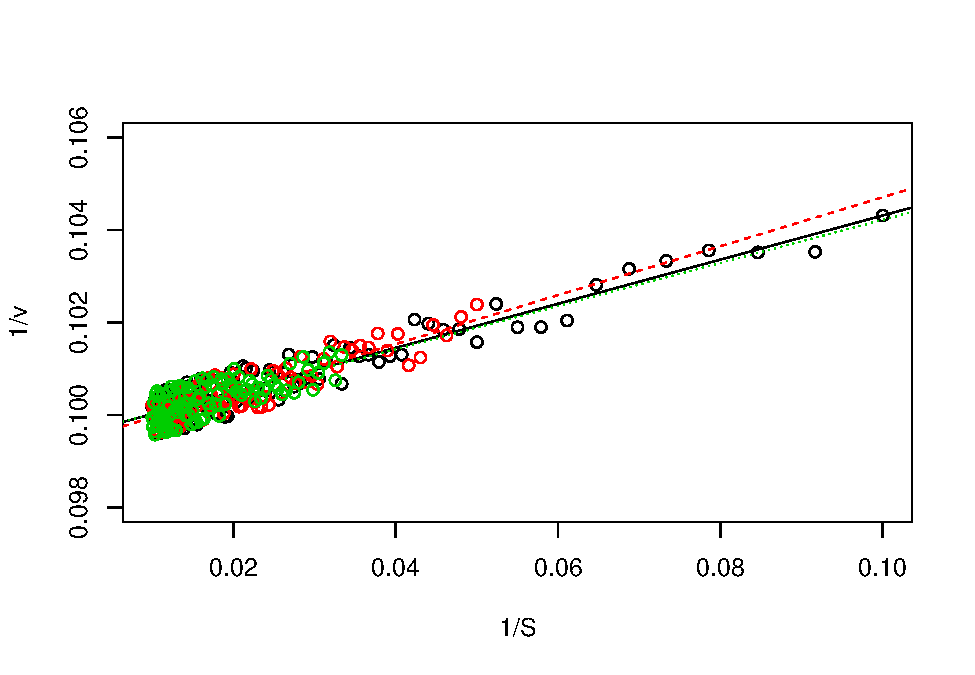
\includegraphics{Bioquímica-Quantitativa-com-R_files/figure-latex/diffLB-1.pdf}
\caption{\label{fig:diffLB}Gráficos duplo-recíproco para a curva simulada de Michaelis-Menten, para distintos teores de S inicial.}
\end{figure}

~~~~~~Observe agora que pela figura \ref{fig:diffLB} resultante, tanto o intercepto como a inclinação obtidos a partir dos ajustes foram dependentes da faixa de seleção de \emph{S}, o que resulta em distintos valores para \emph{Vm} e \emph{Km}. Isto mostra como a seleção da faixa de \emph{S} para o cálculo de \emph{Km} e \emph{Vm} é crucial.

\hypertarget{linearizauxe7uxe3o-por-transformauxe7uxe3o-de-eadie-hofstee}{%
\subsection{Linearização por transformação de Eadie-Hofstee}\label{linearizauxe7uxe3o-por-transformauxe7uxe3o-de-eadie-hofstee}}

~~~~~~Como já mencionado, as duas linearizações da equação de Michaelis-Menten mais comuns referem-se à do subtítulo acima. A equação de linearização de Eadie-Hosftee é dada abaixo:

\begin{equation}
v = \frac{1}{Km} * \frac{v}{S} + Vm
\label{eq:eqEH}
\end{equation}

~~~~~~A partir dos dados da figura \ref{fig:simulMM} obtém-se os parâmetros cinéticos diretamente do intercepto (Vm) e da inclinação linear (1/Km) por:

\begin{lstlisting}[language=R]
Vm=10; Km=0.5
set.seed(1500) # semente fixa para erro aleatório
erro=runif(length(S),0,0.1)
S=seq(1,10,0.1)
v=Vm*S/(Km+S)+erro
v.S=v/S
plot(v.S~v, xlab="v", ylab="v/S")

lm_EH<-lm(v.S~v); summary(lm_EH)
\end{lstlisting}

\begin{lstlisting}
## 
## Call:
## lm(formula = v.S ~ v)
## 
## Residuals:
##     Min      1Q  Median      3Q     Max 
## -0.1160 -0.0650  0.0117  0.0546  0.1248 
## 
## Coefficients:
##             Estimate Std. Error t value Pr(>|t|)    
## (Intercept) 20.31073    0.07906     257   <2e-16 ***
## v           -2.02191    0.00893    -226   <2e-16 ***
## ---
## Signif. codes:  0 '***' 0.001 '**' 0.01 '*' 0.05 '.' 0.1 ' ' 1
## 
## Residual standard error: 0.07 on 98 degrees of freedom
## Multiple R-squared:  0.998,  Adjusted R-squared:  0.998 
## F-statistic: 5.13e+04 on 1 and 98 DF,  p-value: <2e-16
\end{lstlisting}

\begin{lstlisting}[language=R]
abline(lm_EH, col="blue")
\end{lstlisting}

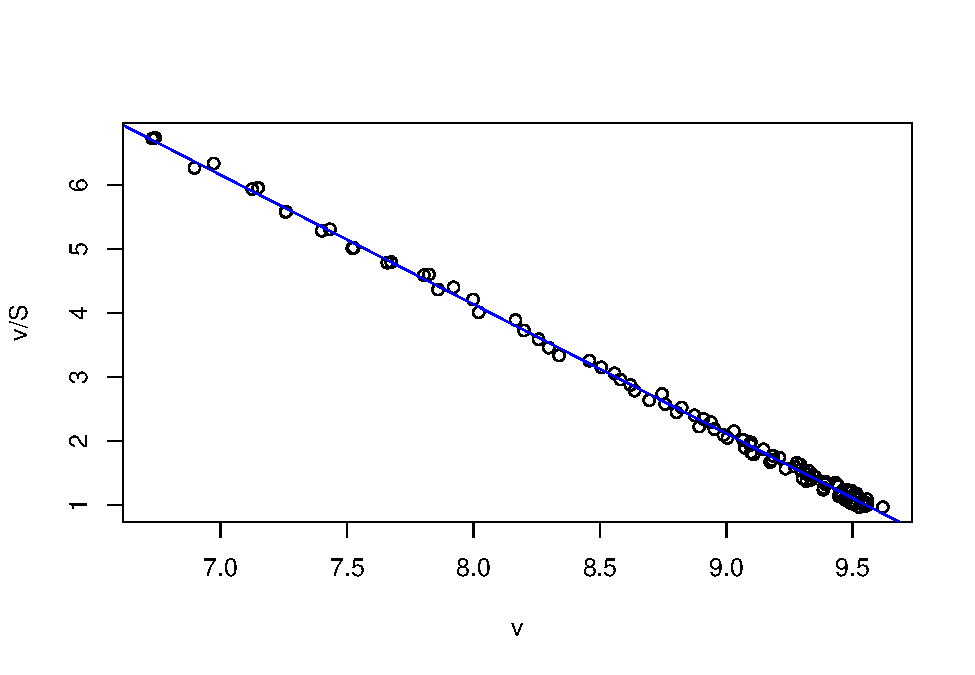
\includegraphics{Bioquímica-Quantitativa-com-R_files/figure-latex/plotEH-1.pdf}

\hypertarget{distribuiuxe7uxe3o-de-erros-nas-linearizauxe7uxf5es-de-michaelis-mentem}{%
\subsection{Distribuição de erros nas linearizações de Michaelis-Mentem}\label{distribuiuxe7uxe3o-de-erros-nas-linearizauxe7uxf5es-de-michaelis-mentem}}

~~~~~~Embora ambas as representações, Lineweaver-Burk e Eadie-Hofstee, sejam as mais utilizadas e apresentem semelhança na obtenção dos parâmetros cinéticos, sua distribuição de resíduos é bem distinta, assim como as demais transformações lineares de Michaelis-Mentem (figura \ref{fig:figLin}).\\
\hspace*{0.333em}\hspace*{0.333em}\hspace*{0.333em}\hspace*{0.333em}\hspace*{0.333em}\hspace*{0.333em}O código abaixo ilustra a distribuição de erros dessas transformações, introduzindo uma função importante do \passthrough{\lstinline!R!} para construção de gráficos com \emph{barras de erros}: \passthrough{\lstinline!arrows!}.

\begin{lstlisting}[language=R]
Vm=10; Km=0.5 # fixa os parâmetros de MM
set.seed(1500) # fixa semente para erro aleatório
erro=runif(length(S),0,0.5) # vetor de erro uniforme
S=c(0.1,0.2,0.5,1,5,10,20) # vetor de substrato
v=Vm*S/(Km+S) # equação de MM
par(mfrow=c(2,2)) # área de plot pra 4 gráficos
plot(S,v,type="o",main="Michaelis-Mentem")
arrows(S,v,S,v-erro,length=.05,angle=90) # barra inferior de erro
arrows(S,v,S,v+erro,length=.05,angle=90) # barra superior de erro

plot(1/S,1/v,type="o",main="Lineweaver-Burk")
arrows(1/S,1/v,1/S,1/(v-erro),length=.05,angle=90)
arrows(1/S,1/v,1/S,1/(v+erro),length=.05,angle=90)

plot(v,v/S,type="o",main="Eadie-Hofstee")
arrows(v,v/S,v,(v-erro)/S,length=.05,angle=90)
arrows(v,v/S,v,(v+erro)/S,length=.05,angle=90)

plot(S,S/v,type="o",main="Hanes-Woolf")
arrows(S,S/v,S,S/(v-erro),length=.05,angle=90)
arrows(S,S/v,S,S/(v+erro),length=.05,angle=90)
\end{lstlisting}

\begin{figure}
\centering
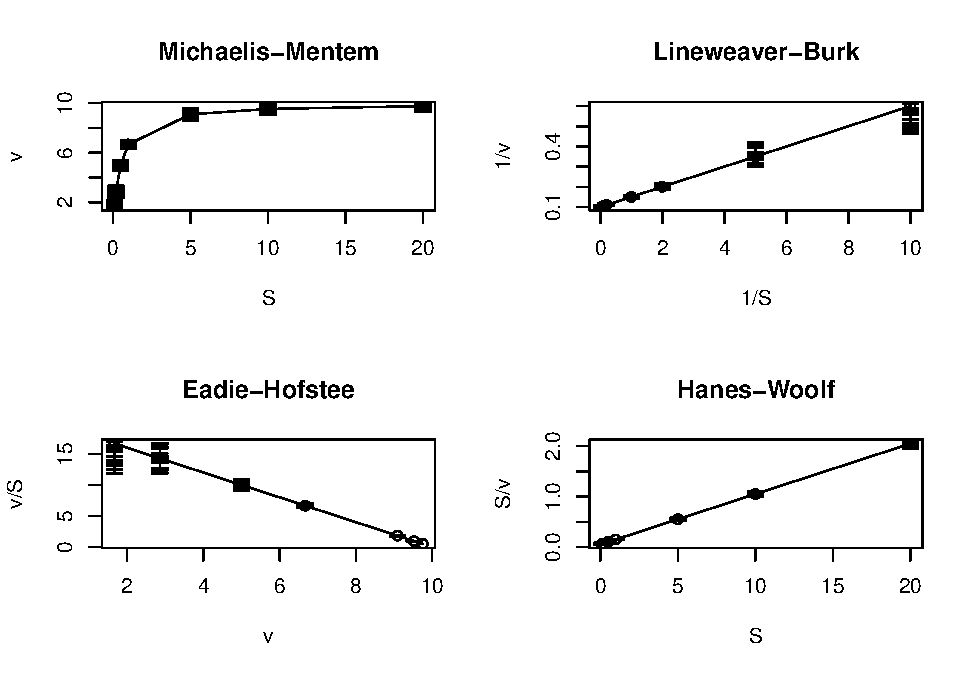
\includegraphics{Bioquímica-Quantitativa-com-R_files/figure-latex/figLinErr-1.pdf}
\caption{\label{fig:figLinErr}Distribuição de erros aleatórios para a equação de Michaelis-Mentem e suas transformações lineares.}
\end{figure}

\begin{lstlisting}[language=R]
par(mfrow=c(1,1)) # retorno à janela gráfica normal
\end{lstlisting}

~~~~~~Pelo gráfico da figura \ref{fig:figLinErr} fica evidente que as transformações de Lineweaver-Burk e de Eadie-Hofstee, ainda que tenham prevalência na literatura, são as que apresentam a maior variabilidade de erro a partir dos dados experimentais, o que converge para uma menor precisão na determinação de parâmetros cinéticos. Além disso, observa-se que a transformação de Hanes-Woolf é a que apresenta a menor dispersão de resíduos entre as demais, igualando-se aos erros experimentais da equação hiperbólica de Michaelis-Mentem. Apesar disso, a linearização de Hanes-Woolf é muito pouco reportada na literatura.\\
\hspace*{0.333em}\hspace*{0.333em}\hspace*{0.333em}\hspace*{0.333em}\hspace*{0.333em}\hspace*{0.333em}Ainda que a representação dos duplos-recíprocos tenha em si algumas desvantagens, tais como a dispersão de erros principalmente em valores baixos de \emph{S}, é a única dentre as mencionadas que permite um ajuste linear por mínimos quadrados, se considerarmos as premissas estatísticas desse.\\
\hspace*{0.333em}\hspace*{0.333em}\hspace*{0.333em}\hspace*{0.333em}\hspace*{0.333em}\hspace*{0.333em}Para que se possa obter parâmetros de intercepto e inclinação a partir de uma regressão linear, é necessário que se cumpra as \emph{premissas estatísticas} de 1) distribuição normal de resíduos, 2) homogeneidade de variâncias, e 3) independência das variáveis. Se observarmos as três linearizações, tanto a de Eadie-Hofstee como a de Hanes-Woolf não cumprem a premissa de independência, já que a variável dependente (y) é função da independente (x).\\
\hspace*{0.333em}\hspace*{0.333em}\hspace*{0.333em}\hspace*{0.333em}\hspace*{0.333em}\hspace*{0.333em}Para que uma transformação por duplos-recíprocos possa ser utilizada mais fielmente à obtenção de parâmetros cinéticos, contudo, pode-se adotar o cômputo de peso na fórmula de ajuste linear, tal como sugerido por Wilkinson \citep{wilkinson1961statistical}, considerando-o como o recíproco das variâncias estimadas. Nesse caso, o ajuste linear considerando o quadrado do vetor de erros aleatórios como variância e o peso como seu recíproco (1/s²), pode ser esboçado como:

\begin{lstlisting}[language=R]
S=seq(0.1,1,length.out=20)
Vm=10; Km=0.5 
set.seed(1500) 
erro=runif(20,0,1)
v=Vm*S/(Km+S)+erro 
inv.S=1/S 
inv.v=1/v
reg.LB.peso<-lm(inv.v~inv.S, weights=1/erro^2) # expressão para ajuste linear
summary(reg.LB.peso) # resultados do ajuste
\end{lstlisting}

\begin{lstlisting}
## 
## Call:
## lm(formula = inv.v ~ inv.S, weights = 1/erro^2)
## 
## Weighted Residuals:
##      Min       1Q   Median       3Q      Max 
## -0.04779 -0.02231 -0.01849  0.00162  0.04830 
## 
## Coefficients:
##             Estimate Std. Error t value Pr(>|t|)    
## (Intercept)  0.11733    0.00254    46.1  < 2e-16 ***
## inv.S        0.03491    0.00145    24.0  3.9e-15 ***
## ---
## Signif. codes:  0 '***' 0.001 '**' 0.01 '*' 0.05 '.' 0.1 ' ' 1
## 
## Residual standard error: 0.03 on 18 degrees of freedom
## Multiple R-squared:  0.97,   Adjusted R-squared:  0.968 
## F-statistic:  578 on 1 and 18 DF,  p-value: 3.93e-15
\end{lstlisting}

~~~~~~Ainda que os ajustes tenham sido realizados para valores com baixa variabilidade de erros uniformes, uma comparação entre esse resultado e o da figura \ref{fig:figLBlin} revela ligeira superioridade para o primeiro, com maior valor para o coeficiente de determinação \emph{R²}, menor para \emph{p-valor}, e menores para o \emph{erro-padrão} das estimativas.\\
\hspace*{0.333em}\hspace*{0.333em}\hspace*{0.333em}\hspace*{0.333em}\hspace*{0.333em}\hspace*{0.333em}Complementarmente, pode-se obter uma comparação estatística entre o modelo linear simples e o que adotou o peso estatístico por:

\begin{lstlisting}[language=R]
anova(reg.LB,reg.LB.peso)
\end{lstlisting}

\begin{lstlisting}
## Analysis of Variance Table
## 
## Model 1: inv.v ~ inv.S
## Model 2: inv.v ~ inv.S
##   Res.Df     RSS Df Sum of Sq F Pr(>F)
## 1     18 0.00383                      
## 2     18 0.01585  0    -0.012
\end{lstlisting}

\hypertarget{ajuste-nuxe3o-linear}{%
\section{Ajuste não-linear}\label{ajuste-nuxe3o-linear}}

~~~~~~Ainda que linearizações sejam frequentemente utilizadas mesmo hoje em dia, principalmente para discernir entre modelos cinéticos distintos, a determinação precisa dos parâmetros de catálise é contudo melhor conduzida por ajuste ou regressão não-linear. Esse ajuste tem por objetivo a determinação de parâmetros de uma equação (\emph{Vm} e \emph{Km}, no caso) sem a necessidade de qualquer transformação dos dados, eliminando por essa razão os erros associados.\\
\hspace*{0.333em}\hspace*{0.333em}\hspace*{0.333em}\hspace*{0.333em}\hspace*{0.333em}\hspace*{0.333em}O ajuste não-linear difere do linear em algumas características, tais como:

\begin{enumerate}
\def\labelenumi{\arabic{enumi}.}
\tightlist
\item
  A busca iterativa de um valor mínimo (local ou global) para a soma dos quadrados dos erros das estimativas;
\item
  a necessidade de um valor inicial para os parâmetros (sementes);
\item
  a linearidade nos erros e no gradiente da função sobre os parâmetros.
\item
  a necessidade de algoritmo mais sofisticado para solução simbólica e matricial para minimizar a derivada da função sobre cada parâmetro;
\item
  a necessidade de programa que trabalhe com álgebra matricial (computador, dispositivo móvel ou calculadora);
\item
  o uso de algoritmos mais sofisticados (Gauss, Newton-Raphson, Levenberg-Marquadt, Simplex).\\
\item
  o emprego da equação original do modelo, por vezes de difícil linearização.
\end{enumerate}

\hypertarget{ajuste-nuxe3o-linear-da-equauxe7uxe3o-de-michaelis-mentem}{%
\subsection{Ajuste não-linear da equação de Michaelis-Mentem}\label{ajuste-nuxe3o-linear-da-equauxe7uxe3o-de-michaelis-mentem}}

~~~~~~Para uma regressão não-linear da equação de Michaelis-Mentem reproduzindo-se a simulação exemplificada na figura \ref{fig:simulMM}:

\begin{lstlisting}[language=R]
Vm=10
Km=0.5
set.seed(1500)  
erro=runif(20,0,1) 
S=seq(0,1,length.out=20)
v=Vm*S/(Km+S)+erro
dat.Sv <- data.frame(S,v) # criação de planilha com S e v
plot(v~S, type="p", from = 0, to=1, n = 20,
      xlab="[S}", ylab="v") # construção do gráfico de MM

nl.MM<-nls(v~Vm*S/(Km+S), start = list(Vm=7, Km=0.2), data=dat.Sv) # linha de código para ajuste não linear
lines(S,fitted(nl.MM),col="red") # sobreposição da linha ajustada
\end{lstlisting}

\begin{figure}
\centering
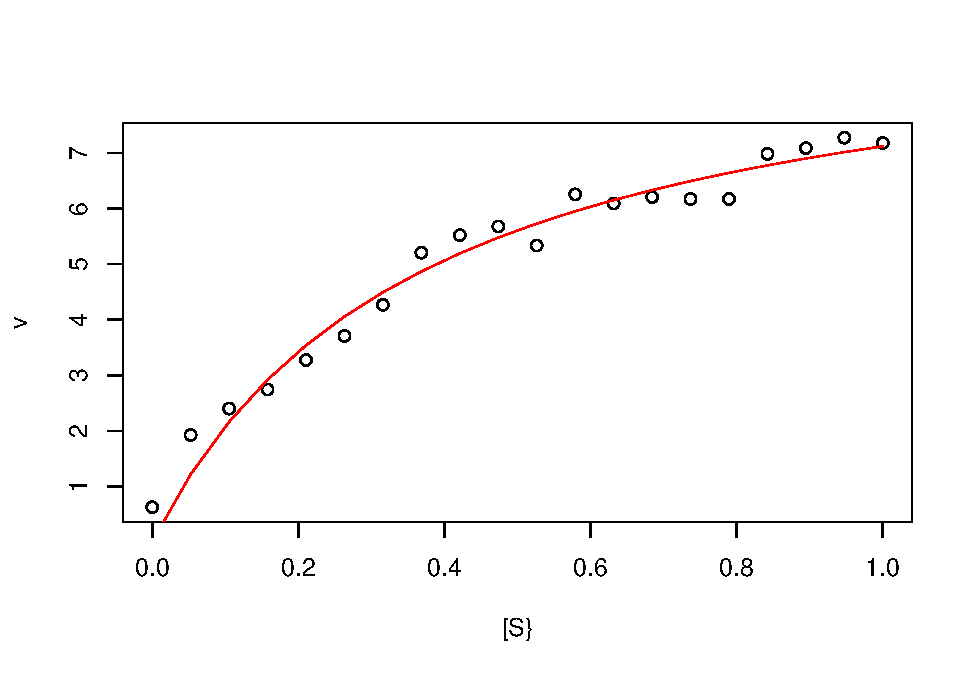
\includegraphics{Bioquímica-Quantitativa-com-R_files/figure-latex/nonlinMM-1.pdf}
\caption{\label{fig:nonlinMM}Ajuste não linear para a simulação experimental da equação de Michaelis-Menten.}
\end{figure}

\begin{lstlisting}[language=R]
summary(nl.MM) # sumário dos resultados
\end{lstlisting}

\begin{lstlisting}
## 
## Formula: v ~ Vm * S/(Km + S)
## 
## Parameters:
##    Estimate Std. Error t value Pr(>|t|)    
## Vm   9.7549     0.5211   18.72  3.0e-13 ***
## Km   0.3698     0.0502    7.37  7.7e-07 ***
## ---
## Signif. codes:  0 '***' 0.001 '**' 0.01 '*' 0.05 '.' 0.1 ' ' 1
## 
## Residual standard error: 0.4 on 18 degrees of freedom
## 
## Number of iterations to convergence: 5 
## Achieved convergence tolerance: 1.6e-06
\end{lstlisting}

~~~~~~Observe agora pela tabela de sumário do ajuste que os parâmetros são fornecidos diretamente, sem necessidade de transformação, como no ajuste linear. A tabela diferencia-se do sumário de ajuste linear por apresentar o número de iterações para convergência, e o valor de convergência para tolerância. Contudo, não apresenta o coeficiente de determinação \emph{R²}, mas somente o erro padrão residual. Ainda que a discussão esteja longe da proposta desta obra, alguns autores declinam do emprego de \emph{R²} em regressão não-linear pelo mesmo ser decorrente de relações lineares entre os parâmetros, o que não ocorre no caso.\\
\hspace*{0.333em}\hspace*{0.333em}\hspace*{0.333em}\hspace*{0.333em}\hspace*{0.333em}\hspace*{0.333em}Assim como para ajuste linear, os parâmetros que abrangem a função \passthrough{\lstinline!nls!} envolvem:

\begin{lstlisting}[language=R]
args(nls)
\end{lstlisting}

\begin{lstlisting}
## function (formula, data = parent.frame(), start, control = nls.control(), 
##     algorithm = c("default", "plinear", "port"), trace = FALSE, 
##     subset, weights, na.action, model = FALSE, lower = -Inf, 
##     upper = Inf, ...) 
## NULL
\end{lstlisting}

~~~~~~Além do pacote incluido na distribuição básica do \passthrough{\lstinline!R!} e que permite ajustes não-lineares (\passthrough{\lstinline!stats!}), existem diversos outros que permitem ajustes com algoritmos, avaliações e plotagens variadas, tais como \passthrough{\lstinline!nlme!} (\emph{mixed-effects}), \passthrough{\lstinline!nlrwr!}, \passthrough{\lstinline!nlstools!}, \passthrough{\lstinline!nls2!}, \passthrough{\lstinline!nls.multstart!}, \passthrough{\lstinline!minpack.lm!} (algoritmo de Levenberg-Marquadt), \passthrough{\lstinline!nlshelper!}, e \passthrough{\lstinline!nlsLM!}.

\hypertarget{algumas-vantagens-do-modelo-linear-sobre-o-nuxe3o-linear}{%
\subsection{Algumas vantagens do modelo linear sobre o não-linear}\label{algumas-vantagens-do-modelo-linear-sobre-o-nuxe3o-linear}}

~~Ainda que a estimativa de parâmetros de modelos não lineares seja mais precisa utilizando-se ajustes também não lineares, o algoritmo linear oferece algumas vantagems, entre as quais:

\begin{enumerate}
\def\labelenumi{\arabic{enumi}.}
\tightlist
\item
  É mais fácil, com algoritmo simplificado, e mesmo pelo uso de somatórias de algumas quantidades envolvendo \emph{x} e \emph{y}, sendo resolvido com calculadora científica simples, ou mesmo à mão;
\item
  é mais intuitivo visualmente, posto que o modelo final será sempre uma reta;
\item
  possui apenas dois parâmetros na equação, intercepto e inclinação;
\item
  requer poucas medidas, já que uma reta se constroi com apenas dois pontos;
\item
  não requer sementes para estimativas iniciais o que, a depender do modelo não-linear, pode ser bem abstrato, culminando em mínimos locais ou mesmo na falta de solução para o ajuste;
\item
  permite interpretação experimental quando há fuga da linearidade;
\item
  independe de um modelo físico específico;
\item
  não requer, por vezes, a necessidade de constrição de resultados (\emph{constraints}), por exemplo instruindo o algoritmo a buscar uma estimativa obrigatoriamente de valor positivo para o parâmetro.
\item
  relações lineares e transformações são encontradas em inúmeros modelos físicos nas Ciências Naturais.
\end{enumerate}

\hypertarget{enzimas-alostuxe9ricas}{%
\section{Enzimas alostéricas}\label{enzimas-alostuxe9ricas}}

~~~~~~A \emph{alosteria} constitui um dos principais recursos da metabolismo para a regulação dos níveis de compostos celulares. De etiologia grega (\emph{allos = outro, stereos = estrutura}), uma \emph{enzima alostérica} é aquela que altera seu perfil catalítico em função de transições conformacionais mediadas por moléculas que interagem fora de seu sítio ativo, sejam elas substrato, coenzimas, ou outros compostos \citep{traut2007allosteric}. O efeito resultante constitui em uma modulação da atividade enzimática, quer ativando-a ou inibindo-a. Enzimas alostérica comportam-se portanto como \emph{enzimas regulatórias} em uma rota metabólica, e cuja atividade pode ser modulada em função de \emph{retroinibição} ou \emph{inibição por feedback}, bem como por \emph{ativação pelo precursor} \citep{defundamentos}.\\
\hspace*{0.333em}\hspace*{0.333em}\hspace*{0.333em}\hspace*{0.333em}\hspace*{0.333em}\hspace*{0.333em}A equação que define uma enzima alostérica em função do teor de seu substrato dada abaixo:

\begin{equation}
v=\frac{Vm*S^n}{(Km^n+S^n)}
\label{eq:eqLB}
\end{equation}

Onde \emph{nH} representa o \emph{coeficiente de cooperatividade ou constante de Hill} para a ligação com moléculas de \emph{S} (de maneira similar à ligação de \(O_{2}\) à hemoglobina. De modo geral, o valor de \emph{nH} pode ser inferior à unidade (\emph{cooperatividade negativa}) ou superior a essa (\emph{cooperatividade positiva}). Para ilustrar o comportamento cinético de uma enzima alostérica, segue o trecho abaixo, que também introduz outro formato para representar curvas no \passthrough{\lstinline!R!} nomeando a variável independente (\emph{x}).

\begin{lstlisting}[language=R]
v = function(S, Vm=10, Km=3, nH=2) {Vm*S^nH/(Km^nH+S^nH)}
curve(v,from=0,to=10,n=100, xlab="S", ylab="v",
      bty="L") # eixos em L
\end{lstlisting}

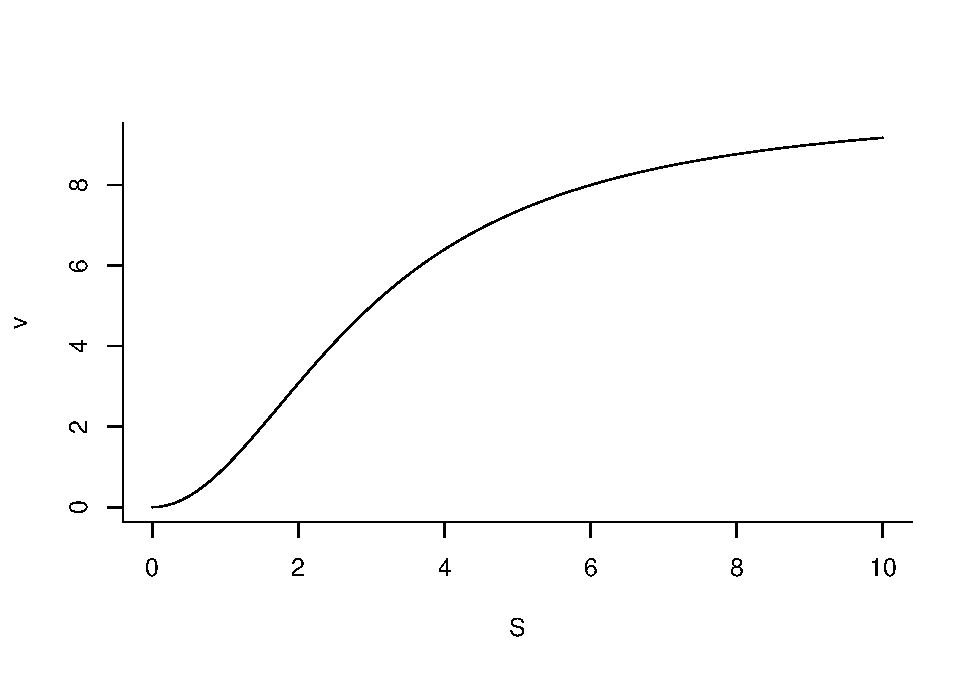
\includegraphics{Bioquímica-Quantitativa-com-R_files/figure-latex/unnamed-chunk-41-1.pdf}

~~Interessante também observar como o perfil enzimático alostérico se define frente à variação do coeficiente \emph{nH}.

\begin{lstlisting}[language=R]
nH=seq(from=0.1,to=3,length.out=7) # sequência para 7 valores de nH
for(i in 1:length(nH)) { # loop para adicionar curva alostérica a cada valor de nH
  add<-if(i == 1) FALSE else TRUE # controle de fluxo
  v = function(S, Vm=10, Km=3, a=nH[i]) {Vm*S^a/(Km^a+S^a)}
  curve(v,from=0,to=4, n=500, col=i, xlab="S", ylab="v",
        bty="L", add=add)
}
arrows(0,5,3,2,length=0.1,angle=45, col="blue") # seta para nH
text(0.5,5.2,"nH",col="blue") # indexador para nH
\end{lstlisting}

\begin{figure}
\centering
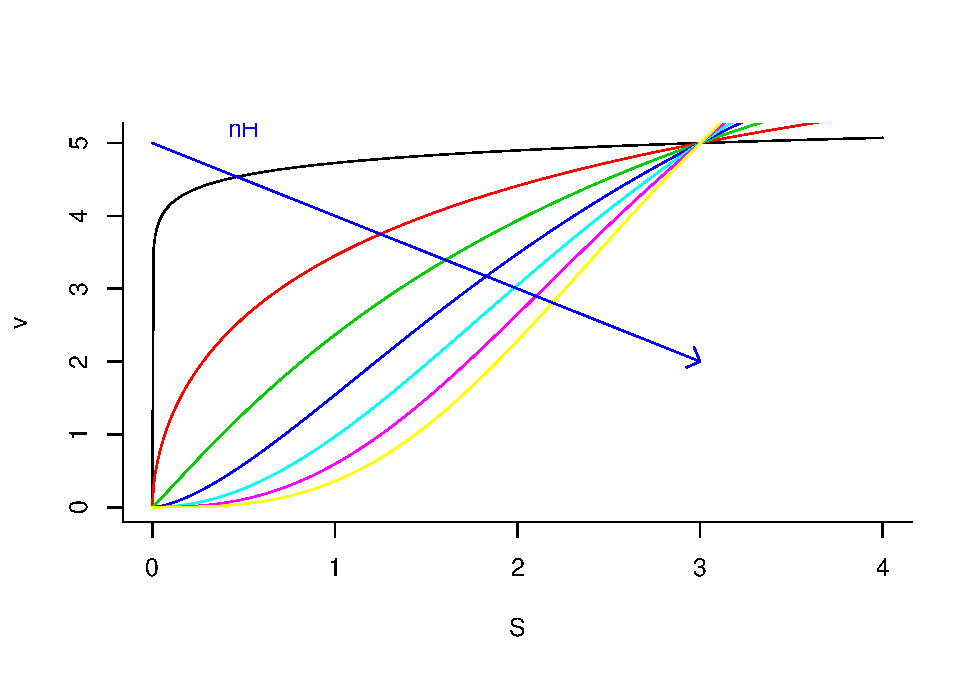
\includegraphics{Bioquímica-Quantitativa-com-R_files/figure-latex/figAlosN-1.pdf}
\caption{\label{fig:figAlosN}Perfil alostérico de uma enzima sob variação do coeficiente de cooperatividade nH.}
\end{figure}

\hypertarget{inibiuxe7uxe3o-enzimuxe1tica}{%
\section{Inibição Enzimática}\label{inibiuxe7uxe3o-enzimuxe1tica}}

~~~~~~Capítulo vasto na enzimologia e com aplicação direta em Química, Farmacologia, Biotecnologia, Biomedicina e áreas afins, a inibição enzimática encontra-se no âmago dos fármacos, medicamentos e biosensores. Sob um ponto de vista simplificado, a atividade enzimática pode ser reduzida na presença de vários efetores, entre moléculas endógenas ou exógenas do metabolismo celular, incluindo o próprio substrato. Genericamente a \emph{inibição enzimática} classifica-se como \emph{irreversível} quando a ativide decai pela ligação covalente de um inibidor, ou \emph{reversível}, quando há um equilíbrio de associação/dissociação com a macromolécula. A seguir serão ilustradas inibições reversíveis.

\hypertarget{inibiuxe7uxe3o-pelo-substrato}{%
\subsection{Inibição pelo substrato}\label{inibiuxe7uxe3o-pelo-substrato}}

~~~~~~Uma inibição enzimática comum ao metabolismo é a protagonizada pelo próprio substrato em excesso no meio, sendo definida por:

\begin{equation}
v=\frac{Vm*S}{S(1+\frac{S}{Ks})+Km}
\label{eq:eqInibS}
\end{equation}

~~~~~~Dessa forma, o gráfico resultante de uma inibição por excesso de substrato pode ser reproduzido por:

\begin{lstlisting}[language=R]
S=seq(0,10,0.1)
v_alos <- function(S, Vm=10, Km=0.5, Ks=2) {Vm*S/(S*(1+S/Ks)+Km)}
curve(v_alos, xlim=c(0,10), xlab="S",ylab="v")
\end{lstlisting}

\begin{figure}
\centering
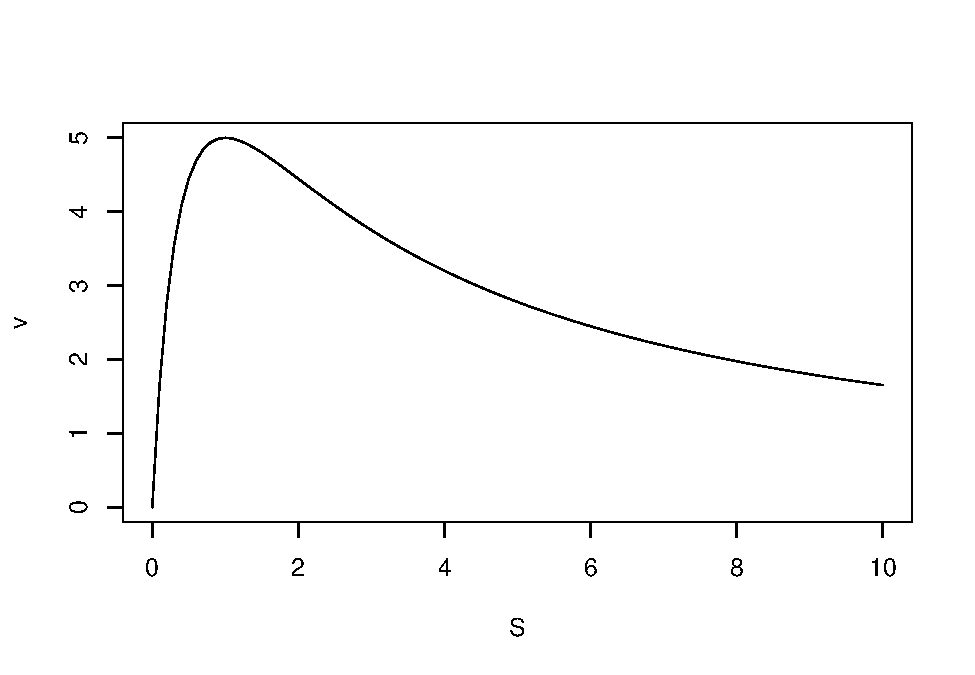
\includegraphics{Bioquímica-Quantitativa-com-R_files/figure-latex/figInibS-1.pdf}
\caption{\label{fig:figInibS}Comportamento cinético de uma enzima inibida por excesso de substrato.}
\end{figure}

~~~~~~Percebe-se pela figura \ref{fig:figInibS} que a atividade da enzima alcança um limite sendo reduzida com o aumento do teor de substrato.

\hypertarget{modelos-de-inibiuxe7uxe3o-enzimuxe1tica}{%
\subsection{Modelos de inibição enzimática}\label{modelos-de-inibiuxe7uxe3o-enzimuxe1tica}}

~~~~~~A inibição de enzimas por moléculas que não o próprio substrato pode ser representada por um diagrama no qual o efetor altera um dos elementos representados na equação \eqref{eq:diagMM}, tal como na figura abaixo.

\hfill\break

\begin{figure}
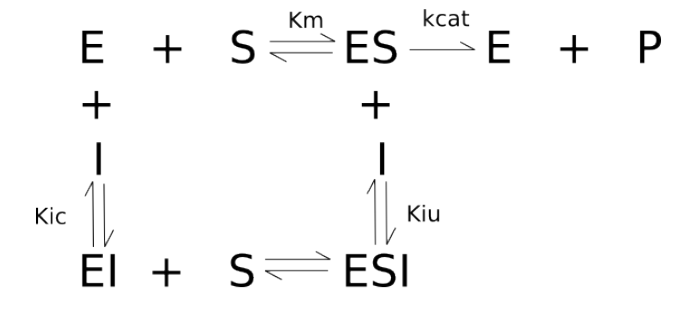
\includegraphics[width=0.6\linewidth]{figures/inibDiag} \caption{Diagrama representativo dos tipos de inibição enzimática. kcat: constante catalítica; Ki: constante de equilíbrio de dissociação do inibidor, com índices para inibição competitiva (Ki), incompetitiva (Kiu) e não competitiva (Kic e Kiu).}\label{fig:inibDiag}
\end{figure}

~~~~~~Nesse caso, pode-se definir os três tipos principais de inibição enzimática reversível como \emph{inibição competitiva, incompetitiva e não competitiva (pura ou mista)}. Em síntese, a \emph{inibição competitiva} dá-se quando o inibidor complexa-se ao sítio ativo da enzima; a \emph{inibição incompetitiva}, quando o inibidor interage com o complexo enzima-substrato; e a \emph{inibição não competitiva}, quando o inibidor liga-se em outro local que não o sítio ativo da enzima, podendo ainda ser \emph{pura} (Kiu = Kic) ou \emph{mista} (Kiu \textgreater{} ou \textless{} Kic).\\
\hspace*{0.333em}\hspace*{0.333em}\hspace*{0.333em}\hspace*{0.333em}\hspace*{0.333em}\hspace*{0.333em}Um modelo matemático que abrange esses três tipos de inibição enzimática é descrito na equação abaixo:

\begin{equation}
v=\frac{Vm*S}{Km(1+\frac{I}{Kic})+S(1+\frac{I}{Kiu})}
\label{eq:inibAll}
\end{equation}

~~~~~~Dessa forma, a equação \eqref{eq:inibAll} reduz-se em seus termos multiplicadores no denominador, em função do tipo de inibição enzimática presente, até o modelo primitivo de Michaelis-Mentem, quando na ausência do inibidor.\\

\hypertarget{curva-de-michaelis-mentem-para-modelos-de-inibiuxe7uxe3o-enzimuxe1tica}{%
\subsubsection{Curva de Michaelis-Mentem para modelos de inibição enzimática}\label{curva-de-michaelis-mentem-para-modelos-de-inibiuxe7uxe3o-enzimuxe1tica}}

~~~~~~Podemos simular no \passthrough{\lstinline!R!} as cuvas michaelianas para modelos clássicos de inibição, considerando valores para as constantes de equilíbrio de dissociação dos inibidores como Kic = 0.2, e Kiu = 1, como no trecho de código abaixo.

\begin{lstlisting}[language=R]
par(mfrow=c(2,2)) # divide a área de plotagem
S=seq(0,10,0.1) # geração de teores de S
contr <- function(S,Vm=10,Km=0.5) {Vm*S/(Km+S)} # função de MM, sem inibição
curve(contr, xlim=c(0,10), xlab="S",ylab="v",main="Competitiva") # cuva controle; veja que o título tem que ser adicionado para a 1a. de par de curvas, controle e inibição

# Modelos de inibição:

# Competitiva
comp.i <- function(S, Vm=10, Km=0.5, I=2, Kic=0.2) {Vm*S/(Km*(1+I/Kic)+S)}
curve(comp.i, add = TRUE, col="red",lty=2) # competitiva

# Não competitiva pura
pura.i <- function(S, Vm=10, Km=0.5, I=2, Ki=1) {Vm*S/(Km*(1+I/Ki)+S*(1+I/Ki))}
curve(contr, xlim=c(0,10), xlab="S",ylab="v",main="Não Compet. Pura") 
curve(pura.i, add = TRUE, col="red",lty=2) # não competitiva pura (Kiu=Kic=Ki)

# Não competitiva mista
mista.i <- function(S, Vm=10, Km=0.5, I=2, Kic=0.2, Kiu=1) {Vm*S/(Km*(1+I/Kic)+S*(1+I/Kiu))}
curve(contr, xlim=c(0,10), xlab="S",ylab="v",main="Não Compet. Mista") 
curve(mista.i, add = TRUE, col="red",lty=2) # não competitiva mista

# Incompetitiva
incomp.i <- function(S, Vm=10, Km=0.5, I=2, Kiu=1) {Vm*S/(Km+S*(1+I/Kiu))}
curve(contr, xlim=c(0,10), xlab="S",ylab="v",main="Incompetitiva") 
curve(incomp.i, add = TRUE, col="red",lty=2) # incompetitiva
\end{lstlisting}

\begin{figure}
\centering
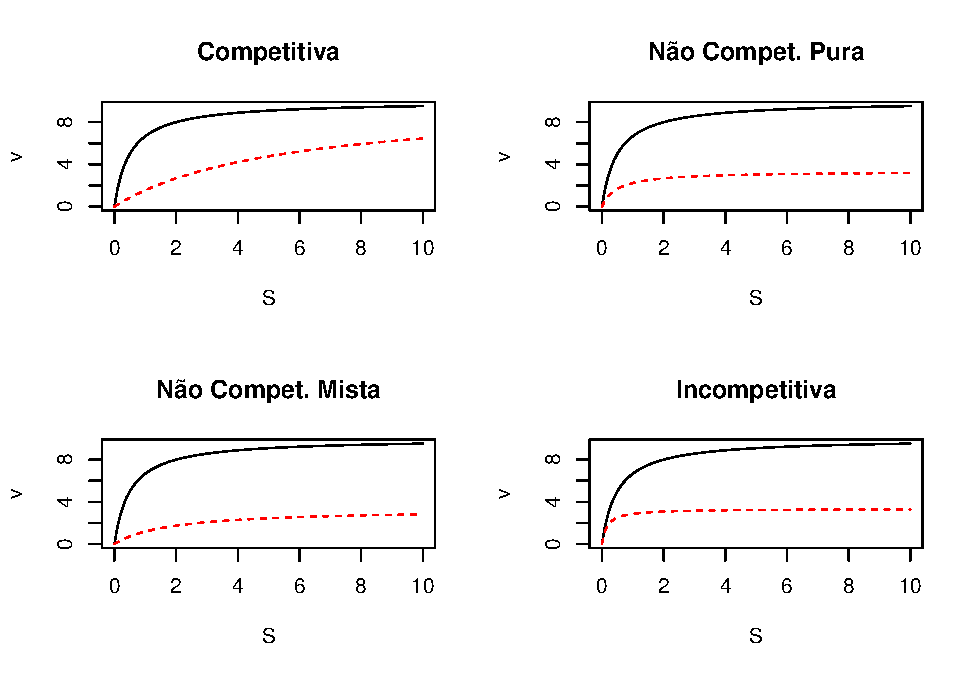
\includegraphics{Bioquímica-Quantitativa-com-R_files/figure-latex/inibMM-1.pdf}
\caption{\label{fig:inibMM}Curva de Michaelis-Mentem na presença de inibidores de comportamento clássico.}
\end{figure}

\begin{lstlisting}[language=R]
layout(1) # retorna à janela gráfica original
\end{lstlisting}

~~~~~~Perceba que para o \emph{modelo competitivo} a velocidade limite \emph{Vm} da reação tende a ser alcançada, já que a ocupação do sítio ativo da enzima é mutualmente exclusiva entre substrato e inibidor, privilegiando o primeiro quando em alto teor. Por outro lado, o valor de \emph{Vm} não é tangível para os demais modelos de inibição, já que o inibidor se liga em outro sítio na enzima (\emph{não competitivo}) ou ao próprio substrato (\emph{incompetitivo}). Para visualizar alterações nos gráficos, experimente modificar os parâmetros da simulação (Vm, Km, Ki, Kic, Kiu, I).\\
\hspace*{0.333em}\hspace*{0.333em}\hspace*{0.333em}\hspace*{0.333em}\hspace*{0.333em}\hspace*{0.333em}Ainda que seja possível um discernimento do modelo competitivo dos demais, perceba também que isso só foi possível por uma simulação que empregou um teor \emph{S} 20 vezes maior que o valor de \emph{Km} da reação. Isso nem sempre é possível na prática, como elencado abaixo, já que o emprego de altos teores de \emph{S}:

\begin{enumerate}
\def\labelenumi{\arabic{enumi}.}
\tightlist
\item
  Agrega maior custo financeiro ao ensaio.
\item
  Pode resultar em inibição por excesso de substrato.
\item
  Pode elevar a viscosidade do meio, reduzindo a taxa catalítica.
\end{enumerate}

~~~~~~Percebe-se, da figura \ref{fig:inibMM} e das observações acima, a dificuldade em classificar o tipo de inibição enzimática baseado na observação direta de uma curva de Michaelis-Mentem.

\hypertarget{diagnuxf3stico-de-modelos-de-inibiuxe7uxe3o-enzimuxe1tica-por-lineweaver-burk}{%
\subsubsection{Diagnóstico de modelos de inibição enzimática por Lineweaver-Burk}\label{diagnuxf3stico-de-modelos-de-inibiuxe7uxe3o-enzimuxe1tica-por-lineweaver-burk}}

~~~~~~As transformações lineares da equação de Michaelis-Mentem são muito úteis no diagnóstico visual de modelos de inibição. Nesse sentido, o emprego da linearização por duplos-recíprocos para esses modelos resutará nas equações de inibição que seguem:

\begin{equation}
\frac{1}{v}=\frac{1}{Vm}+\frac{Km(1+\frac{I}{Kic})}{Vm}*\frac{1}{S} \quad ;\,  competitivo
\label{eq:eqComp}
\end{equation}

\begin{equation}
\frac{1}{v}=\frac{1}{Vm}+\frac{Km(1+\frac{I}{Ki})}{Vm}*\frac{1}{S(1+\frac{I}{Ki})} \quad ;\,  puro
\label{eq:eqPuro}
\end{equation}

\begin{equation}
\frac{1}{v}=\frac{1}{Vm}+\frac{Km(1+\frac{I}{Kic})}{Vm}*\frac{1}{S(1+\frac{I}{Kiu})} \quad ;\,  misto
\label{eq:eqMisto}
\end{equation}

\begin{equation}
\frac{1}{v}=\frac{1}{Vm}+\frac{Km}{Vm}*\frac{1}{S(1+\frac{I}{Kiu})} \quad ;\,  incompetitivo
\label{eq:eqIncomp}
\end{equation}

~~~~~~Observe que os termos multiplicadores inseridos em \emph{S} e \emph{Km} na equação de duplo-recíproco apenas alteram seu formalismo apresentado equação \eqref{eq:eqLB}. Dessa forma, os modelos de inibição enzimática podem ser ilustrados pelo \passthrough{\lstinline!R!} junto à transformação de Lineweaver-Burk (ou qualquer outra), como abaixo.

\begin{lstlisting}[language=R]
# Substrato e Inibidor
S=seq(0.1,10,length=10) # cria um vetor para substrato
I = 2 # concentração de inibidor

# Parâmetros cinéticos:
Km=0.5
Vm=10
Kic=0.2
Ki=0.2
Kiu=1

# Equações
v=Vm*S/(Km+S) # equação de MM
v.comp=Vm*S/(Km*(1+I/Kic)+S) # competitivo
v.puro=Vm*S/(Km*(1+I/Ki)+S*(1+I/Ki)) # não competitivo puro
v.misto=Vm*S/(Km*(1+I/Kic)+S*(1+I/Kiu)) # não competitivo misto
v.incomp=Vm*S/(Km+S*(1+I/Kiu))

# Gráficos
par(mfrow=c(2,2)) # área de plot pra 4 gráficos

plot(1/S,1/v,type="l",main="Competitivo",ylim=c(0,2))
points(1/S,1/v.comp, type="l",col="red")
plot(1/S,1/v,type="l",main="Puro",ylim=c(0,5))
points(1/S,1/v.puro, type="l",col="red")
plot(1/S,1/v,type="l",main="Misto",ylim=c(0,2))
points(1/S,1/v.misto, type="l",col="red")
plot(1/S,1/v,type="l",main="Incompetitivo",ylim=c(0,1))
points(1/S,1/v.incomp, type="l",col="red")
\end{lstlisting}

\begin{figure}
\centering
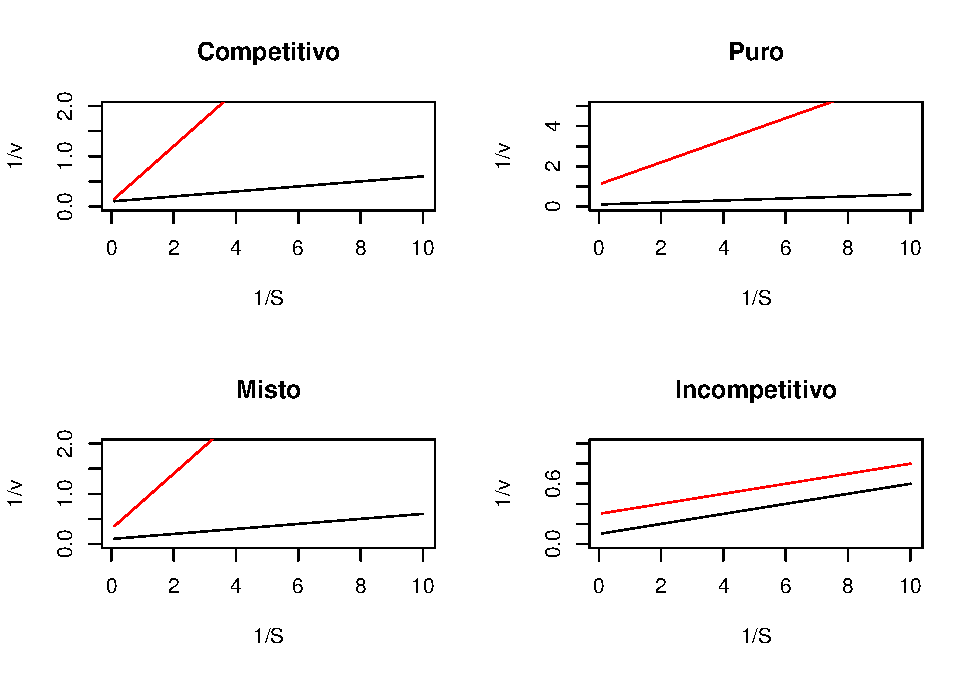
\includegraphics{Bioquímica-Quantitativa-com-R_files/figure-latex/inibLB-1.pdf}
\caption{\label{fig:inibLB}Diagnóstico de modelos de inibição enzimática por Lineweaver-Burk.}
\end{figure}

\begin{lstlisting}[language=R]
layout(1) # volta à janela gráfica normal
\end{lstlisting}

~~~~~~Agora a distinção de modelos de inibição se torna mais evidente pela linearização. Assim como mencionado para os modelos representados na equação direta de Michaelis-Mentem, pode-se variar os parâmetros cinéticos e experimentar a visualização dos duplos-recíprocos.\\
\hspace*{0.333em}\hspace*{0.333em}\hspace*{0.333em}\hspace*{0.333em}\hspace*{0.333em}\hspace*{0.333em}Novamente, ainda que a linearização permita um melhor diagnóstico do tipo de inibição presente, o ajuste não linear é mais adequado para a determinação das constantes de inibição (\emph{Ki'}s), uma vez que não agrega os erros advindos das transformações lineares (embora a inserção de pesos estatísticos possa aliviar a imprecisão dos resultados).

\hypertarget{ki-ic_50}{%
\subsubsection{\texorpdfstring{Ki \& IC\(_{50}\)}{Ki \& IC\_\{50\}}}\label{ki-ic_50}}

~~~~~~A concentração inibitória a 50\% do teor de inibidor, definida como \emph{IC\(_{50}\)}, pode ser determinada empiricamente sem o conhecimento dos parâmetros de catálise enzimática envolvidos. Para isso, basta se obter um valor de inibição relativa num ensaio a concentração fixa de \emph{S}, variando-se o teor de inibidor. De fato, análogos ao \emph{IC\(_{50}\)} existem em ampla gama nas Ciências Naturais, não envolvendo necessariamente qualquer informação cinética ou termodinâmica dos compostos envolvidos, mas tão somente a informação empírica do resultado. Exemplificando, os parâmetros \emph{DE\(_{50}\)} (dose efetiva) ou \emph{DL\(_{50}\)} (dose letal), e mesmo projeções de \emph{X\(_{50}\)}, tal como \emph{Tm} (temperatura de desnaturação a 50\%), e o valor de \emph{pKa} em tampões (pH em que as espécies encontram-se 50\% ionizadas/protonadas em solução).\\
\hspace*{0.333em}\hspace*{0.333em}No entanto, existe uma relação útil entre a constante de equilíbrio de dissociação do inibidor \emph{Ki} e o valor de \emph{IC\(_{50}\)} que permite sua permuta, desde que conhecido o modelo de inibição \citep{yung1973relationship}. Generalizando para os modelos de inibição, pode-se definir uma equação geral pra relação de Cheng-Prusoff como:

\begin{equation}
IC_{50} = \frac{(1+\frac{S}{Km})}{(\frac{1}{Kic})+(\frac{1}{Km*Kiu})}
\label{eq:eqCPrussof}
\end{equation}

~~~~~~Exemplificando, para um \emph{modelo competitivo} de inibição, onde \emph{Kiu} é nulo:

\begin{equation}
IC_{50} = Kic(1+\frac{S}{Km})
\label{eq:eqPrusfComp}
\end{equation}

~~~Como acima mencionado, o valor de \emph{IC\(_{50}\)} pode ser obtido a partir de dados experimentais de inibição relativa (\emph{v/Vm}, por ex) em diferentes concentrações de inibidor fixando um valor de \emph{S}. Nesse caso, podemos ilustrar no \passthrough{\lstinline!R!} a obtenção de \emph{IC\(_{50}\)}, utilizando-se um ajuste não linear para a equação de quatro parâmetros que segue (\emph{curva de Rodbard}, \citet{delean1978simultaneous}).

\begin{equation}
ativ. residual \, \% =\frac{v}{Vm} = inf+\frac{sup-inf}{1+log(\frac{I}{IC_{50}})^{nH}})
\label{eq:eqRodb}
\end{equation}

\begin{lstlisting}[language=R]
logI.nM <- c(5.5,5.2,4.9,4.6,4.3,3.7,3.3,3,2.8) # conc. de I, em unidade log10
ativ.res <- c(0.02,0.07,0.12,0.22,0.36,0.53,0.67,0.83,0.85) # ativ. residual, v/Vm
dados <- data.frame(logI.nM,ativ.res) # criação do dataframe
plot(ativ.res~logI.nM, dados) # plot dos dados
ic50.fit <- nls(formula(ativ.res ~ inf+(sup-inf)/(1+(logI.nM/logIC50)^nH)),algorithm="port", data=dados,start=list(inf=0, sup=0.80, logIC50=4,nH=10), lower=c(inf=-Inf, sup=-Inf, logIC50=0, nH=-Inf) ) # ajuste não linear
summary(ic50.fit) # sumário do ajuste
\end{lstlisting}

\begin{lstlisting}
## 
## Formula: ativ.res ~ inf + (sup - inf)/(1 + (logI.nM/logIC50)^nH)
## 
## Parameters:
##         Estimate Std. Error t value Pr(>|t|)    
## inf       -0.321      0.293   -1.09   0.3235    
## sup        1.120      0.231    4.85   0.0047 ** 
## logIC50    4.081      0.231   17.67  1.1e-05 ***
## nH         4.054      1.746    2.32   0.0679 .  
## ---
## Signif. codes:  0 '***' 0.001 '**' 0.01 '*' 0.05 '.' 0.1 ' ' 1
## 
## Residual standard error: 0.03 on 5 degrees of freedom
## 
## Algorithm "port", convergence message: relative convergence (4)
\end{lstlisting}

\begin{lstlisting}[language=R]
lines(logI.nM,fitted(ic50.fit), col="blue") # linha ajustada
\end{lstlisting}

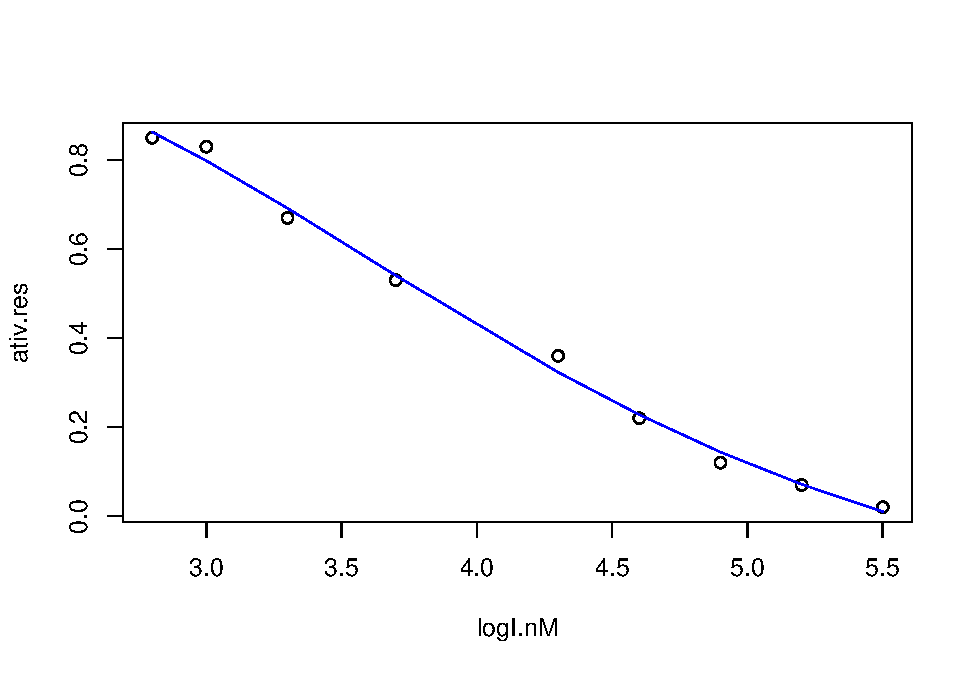
\includegraphics{Bioquímica-Quantitativa-com-R_files/figure-latex/unnamed-chunk-42-1.pdf}

\begin{lstlisting}[language=R]
# E para extrair o valor de IC50...
IC50<-10^(coef(ic50.fit)[3]) # extração do 3o. parâmetro da tabela de ajuste, isto é: logIC50: 
IC50
\end{lstlisting}

\begin{lstlisting}
## logIC50 
##   12042
\end{lstlisting}

~~~~~~Perceba que o parâmetro de \emph{logIC50} foi extraído da tabela de ajuste não linear pelo comando \passthrough{\lstinline!coef!}. Isto é muito útil quando desejamos utilizar um coeficiente obtido em cálculos automáticos (programáveis), como veremos mais adiante. Por ora, faz-se interessante apresentar o parâmetro de \emph{IC50} obtido de forma mais elegante.\\
\hspace*{0.333em}\hspace*{0.333em}\hspace*{0.333em}\hspace*{0.333em}\hspace*{0.333em}\hspace*{0.333em}Para isso, podemos utilizar duas funções do \passthrough{\lstinline!R!} para exprimir resultados quantitativos junto à caracteres (palavras, frases): \passthrough{\lstinline!print()!} e \passthrough{\lstinline!cat!}. O trecho de código abaixo ilustra esse \emph{output}, e algumas diferenças.

\begin{lstlisting}[language=R]
cat("Valor de IC50 (nM):", IC50, "\n")
\end{lstlisting}

\begin{lstlisting}
## Valor de IC50 (nM): 12042
\end{lstlisting}

\begin{lstlisting}[language=R]
print(paste("Valor de IC50 (nM):", IC50))
\end{lstlisting}

\begin{lstlisting}
## [1] "Valor de IC50 (nM): 12042.0412463228"
\end{lstlisting}

~~~~~~Basicamente, \passthrough{\lstinline!print!} exibe aspas e indexa o nome da coluna, enquanto \passthrough{\lstinline!cat!} os omite. Em adição, pode-se perceber outra variação no formato de impressão entre os dois comandos pelo exemplo abaixo:

\begin{lstlisting}[language=R]
print(paste("teores:",c(10,25,50)))
\end{lstlisting}

\begin{lstlisting}
## [1] "teores: 10" "teores: 25" "teores: 50"
\end{lstlisting}

\begin{lstlisting}[language=R]
cat("teores:",c(10,25,50))
\end{lstlisting}

\begin{lstlisting}
## teores: 10 25 50
\end{lstlisting}

~~~~~~Outra possibilidade no \passthrough{\lstinline!R!} é a de se reduzir o número de casas decimais apresentados. Nesse caso, pode-se utilizar o comando \passthrough{\lstinline!round!}.

\begin{lstlisting}[language=R]
IC50<-10^(coef(ic50.fit)[3])
print(paste("Valor de IC50 (nM):", round(IC50,digits=2))) # arredondamento para duas casas decimais
\end{lstlisting}

\begin{lstlisting}
## [1] "Valor de IC50 (nM): 12042.04"
\end{lstlisting}

~~~~~~Mais uma vez, salienta-se a existência de alguns pacotes úteis do \passthrough{\lstinline!R!} para o cálculo de \emph{IC50}, entre esse o pacote \passthrough{\lstinline!drc!} (\emph{dose-response curve}).

\hypertarget{diagnuxf3stico-estatuxedstico-de-inibiuxe7uxe3o-enzimuxe1tica}{%
\section{Diagnóstico estatístico de inibição enzimática}\label{diagnuxf3stico-estatuxedstico-de-inibiuxe7uxe3o-enzimuxe1tica}}

~~~~~~Em paralelo à inspeção visual dos gráficos de linearização para inibição enzimática, é possível validar-se um modelo sobre outro por uma análise de dispersão de erros dos modelos. Mas também é possível o emprego da função \passthrough{\lstinline!BIC!} ou da função \passthrough{\lstinline!AIC!} do \passthrough{\lstinline!R!}, e que respectivamente calculam valores para o \emph{Critério de Informação Bayseiano} \citep{spiess2010evaluation} ou do \emph{Critério de Informação de Akaike} \citep{akaike1974new}. Em comum esse parâmetros calculam um valor relativo de informação não computada por um modelo avaliado. O menor valor encontrado para ambos espelha a solução do melhor modelo de ajuste.\\
\hspace*{0.333em}\hspace*{0.333em}\hspace*{0.333em}\hspace*{0.333em}\hspace*{0.333em}\hspace*{0.333em}Matematicamente, \emph{BIC} e \emph{AIC} podem ser expressos como:

\begin{equation}
BIC = p*ln(n)-2*ln(RSE)\\
\\
AIC = n*ln(\frac{RSE}{n})+2k+[\frac{2k(k+1)}{n-k-1}])\\
\label{eq:BICAIC}
\end{equation}

\textbar Onde \emph{p} representa o no. de parâmetros do modelo, \emph{n} o número total de pontos experimentais, \emph{k} o fator \emph{p+1}, e \emph{RSE} o valor da soma dos quadrados dos resíduos (\emph{residual sum squares}).

~~~~~~Para exemplificar o uso desses parâmetros de qualidade do modelo estatístico, pode-se empregar um conjunto de dados contido no pacote \passthrough{\lstinline!nlstools!}, provendo o ajuste, plotagem, inspeção de resíduos, e aplicação de \emph{BIC} e \emph{AIC}:

\begin{lstlisting}[language=R]
library(nlstools)
\end{lstlisting}

\begin{lstlisting}
## 
## 'nlstools' has been loaded.
\end{lstlisting}

\begin{lstlisting}
## IMPORTANT NOTICE: Most nonlinear regression models and data set examples
\end{lstlisting}

\begin{lstlisting}
## related to predictive microbiolgy have been moved to the package 'nlsMicrobio'
\end{lstlisting}

\begin{lstlisting}[language=R]
comp <- nls(compet_mich, vmkmki, list(Km=1,Vmax=20,Ki=0.5)) # ajuste competitivo, com dados, equação e sementes fornecidas pelo pacote nlstools
plotfit(comp, variable=1) # comando de plotagem do pacote
\end{lstlisting}

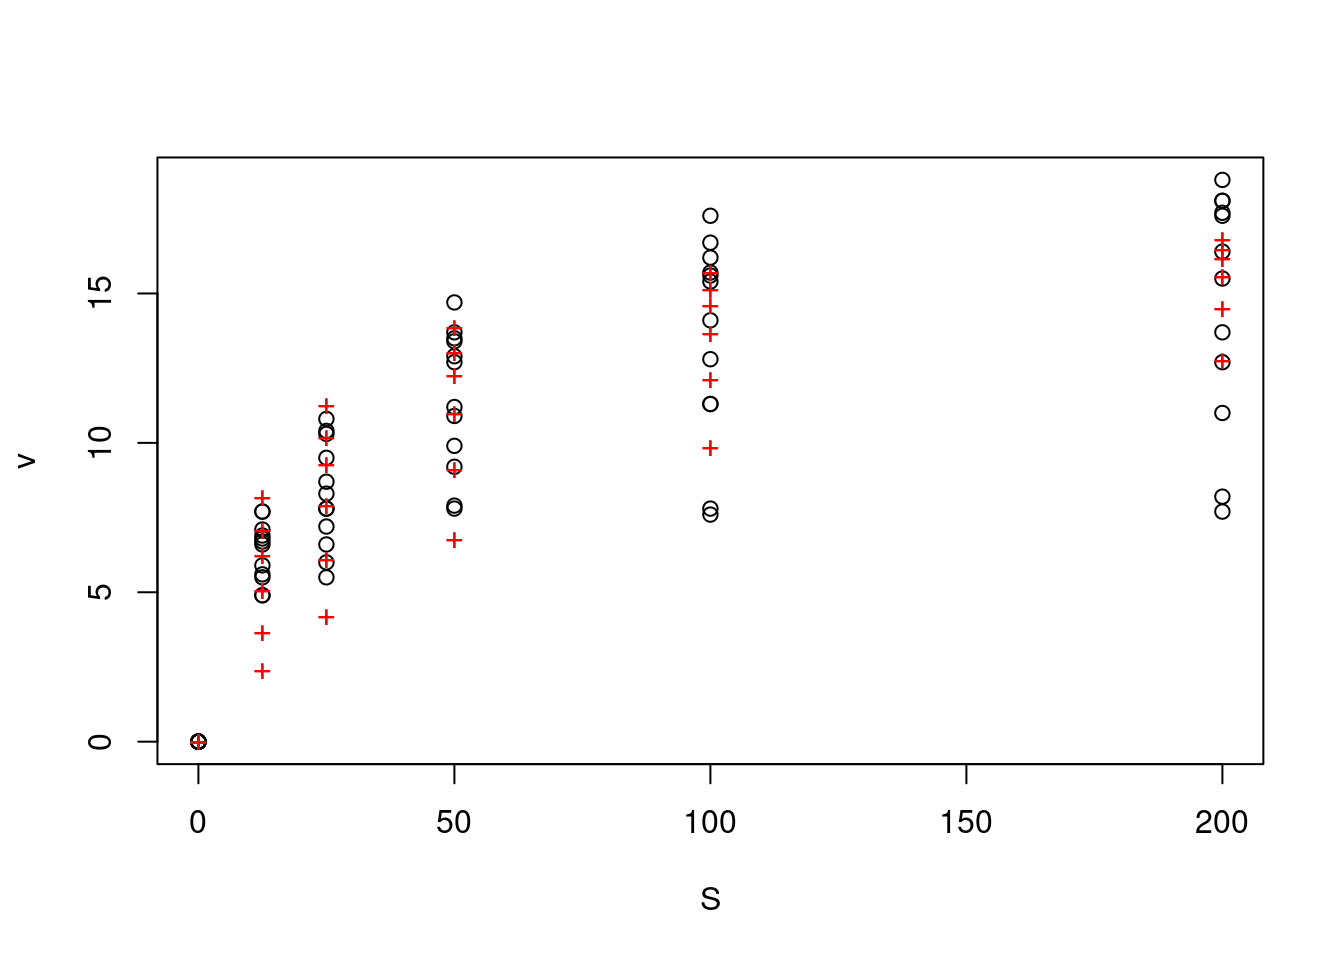
\includegraphics{Bioquímica-Quantitativa-com-R_files/figure-latex/AIC-1.pdf}

\begin{lstlisting}[language=R]
summary(comp)
\end{lstlisting}

\begin{lstlisting}
## 
## Formula: v ~ S/(S + Km * (1 + I/Ki)) * Vmax
## 
## Parameters:
##      Estimate Std. Error t value Pr(>|t|)    
## Km     15.214      2.501    6.08  5.8e-08 ***
## Vmax   18.056      0.629   28.71  < 2e-16 ***
## Ki     22.282      4.906    4.54  2.3e-05 ***
## ---
## Signif. codes:  0 '***' 0.001 '**' 0.01 '*' 0.05 '.' 0.1 ' ' 1
## 
## Residual standard error: 2 on 69 degrees of freedom
## 
## Number of iterations to convergence: 11 
## Achieved convergence tolerance: 5.11e-06
\end{lstlisting}

\begin{lstlisting}[language=R]
res_comp <- nlsResiduals(comp) # resíduos do ajuste
plot(res_comp, which=1) # plotagem de resíduos
\end{lstlisting}

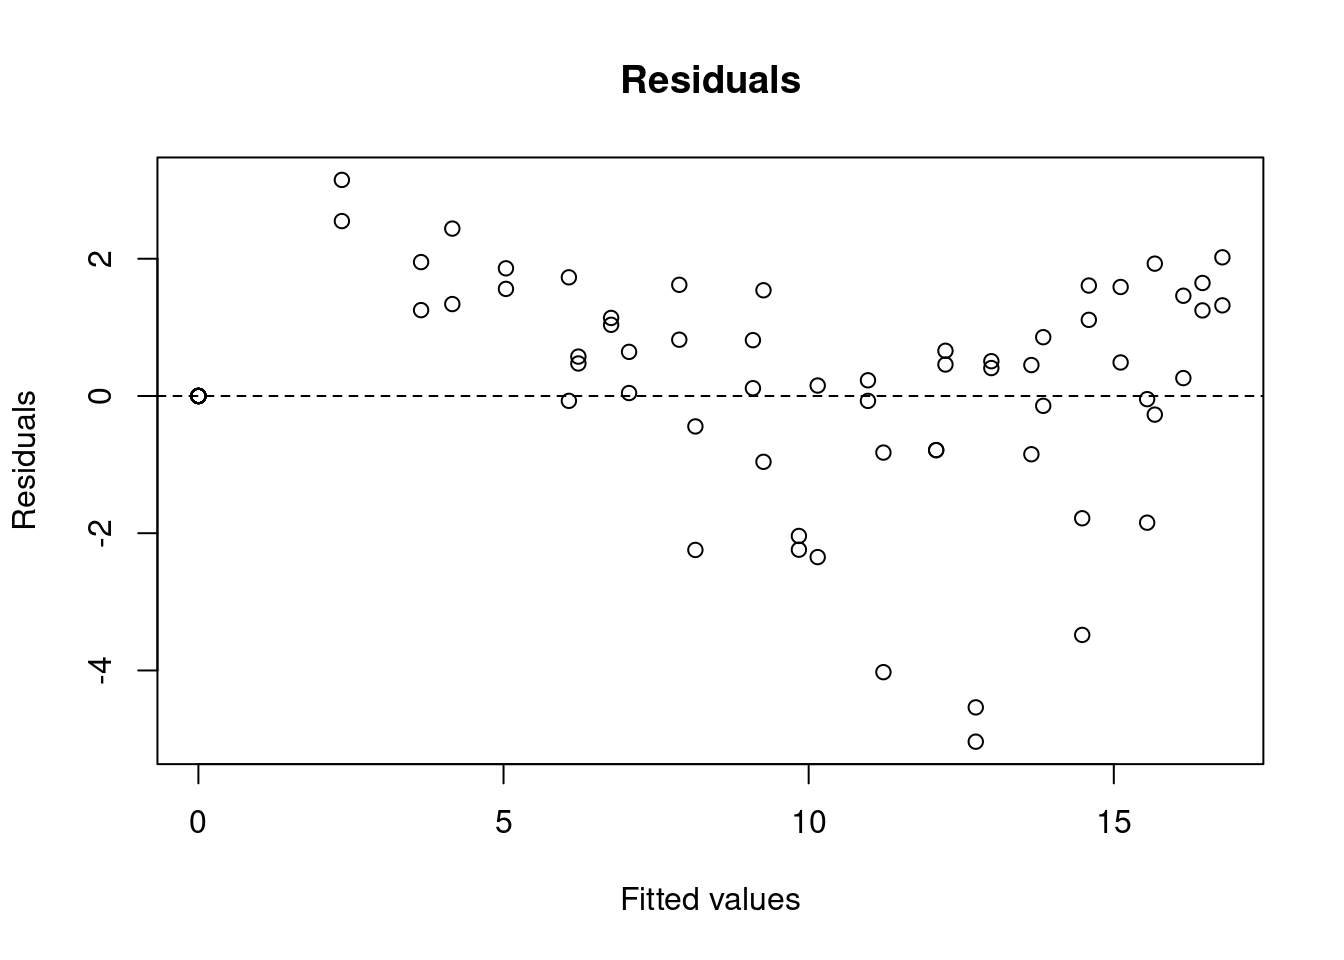
\includegraphics{Bioquímica-Quantitativa-com-R_files/figure-latex/AIC-2.pdf}

\begin{lstlisting}[language=R]
noncomp <- nls(non_compet_mich, vmkmki, list(Km=1, Vmax=20, Ki=0.5)) # o mesmo que acima, mas para o modelo não competitivo
plotfit(noncomp, variable=1)
\end{lstlisting}

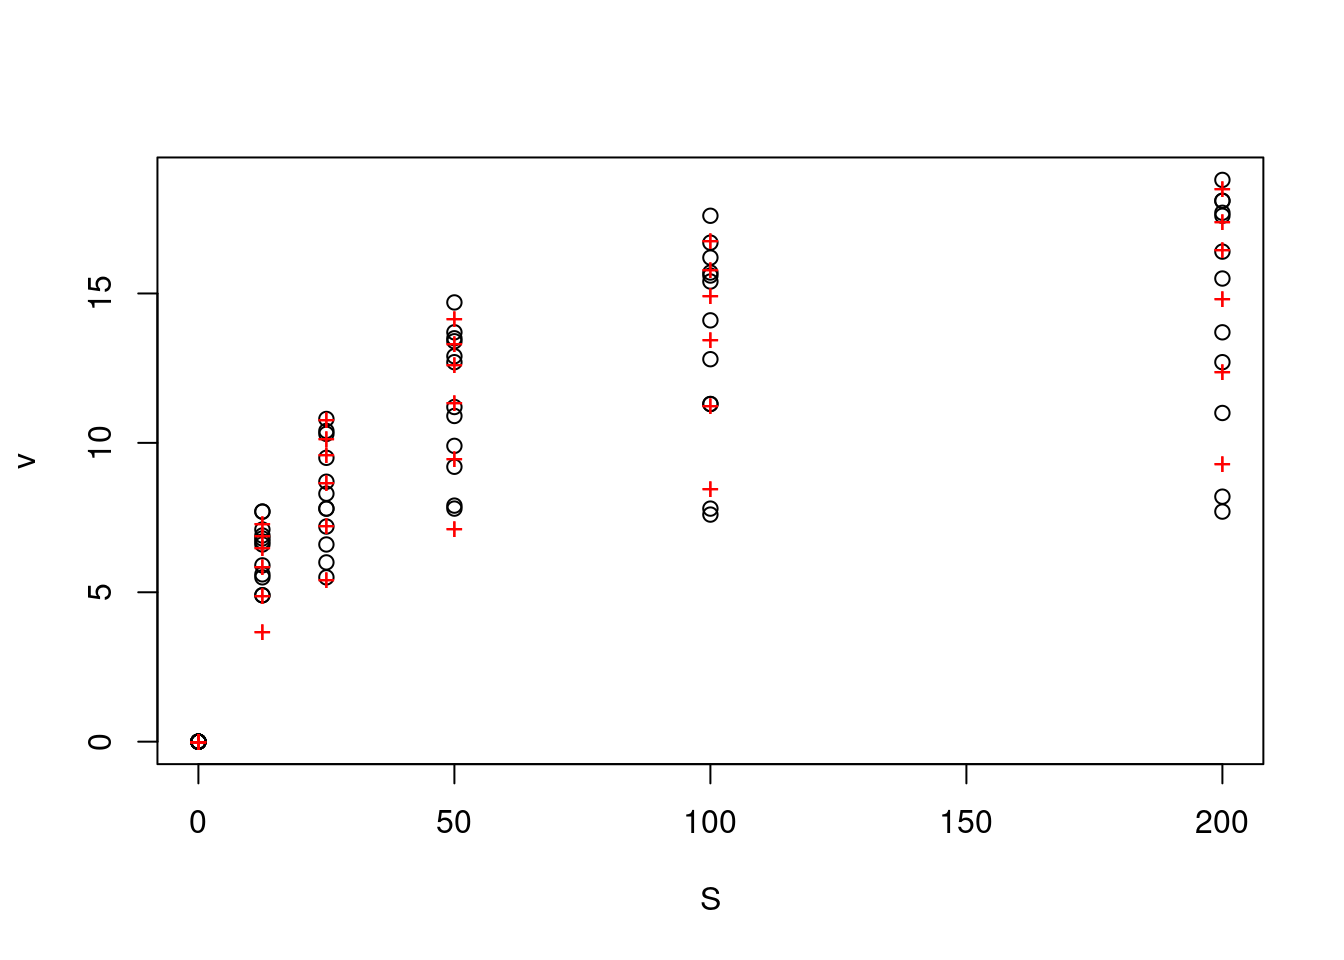
\includegraphics{Bioquímica-Quantitativa-com-R_files/figure-latex/AIC-3.pdf}

\begin{lstlisting}[language=R]
summary(noncomp)
\end{lstlisting}

\begin{lstlisting}
## 
## Formula: v ~ S/((S + Km) * (1 + I/Ki)) * Vmax
## 
## Parameters:
##      Estimate Std. Error t value Pr(>|t|)    
## Km     22.779      1.474    15.5   <2e-16 ***
## Vmax   20.587      0.431    47.8   <2e-16 ***
## Ki    101.356      7.330    13.8   <2e-16 ***
## ---
## Signif. codes:  0 '***' 0.001 '**' 0.01 '*' 0.05 '.' 0.1 ' ' 1
## 
## Residual standard error: 0.9 on 69 degrees of freedom
## 
## Number of iterations to convergence: 7 
## Achieved convergence tolerance: 8.27e-06
\end{lstlisting}

\begin{lstlisting}[language=R]
res_noncomp <- nlsResiduals(noncomp)
plot(res_noncomp, which=1)
\end{lstlisting}

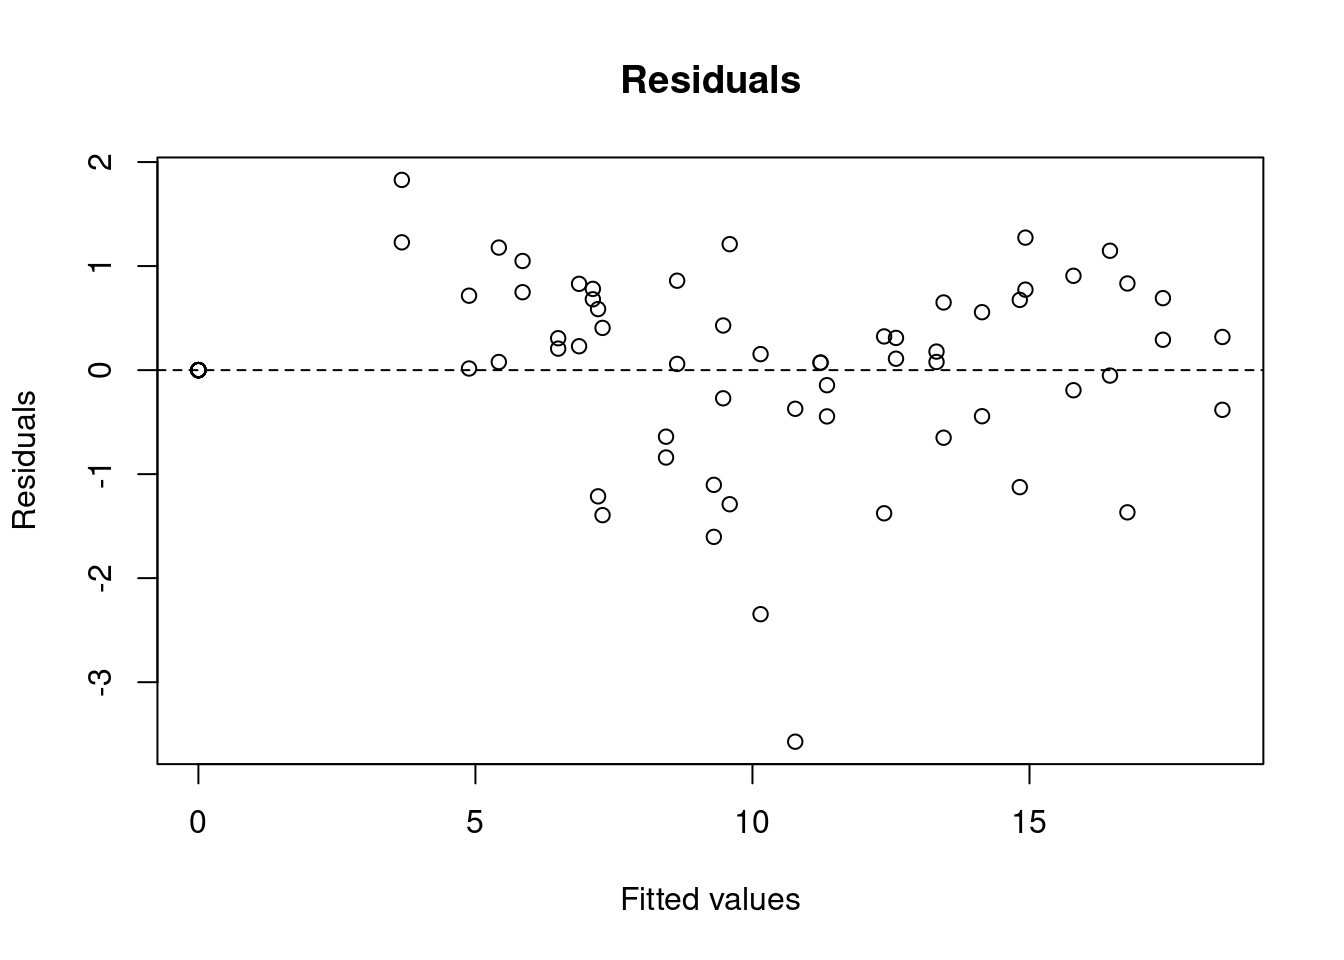
\includegraphics{Bioquímica-Quantitativa-com-R_files/figure-latex/AIC-4.pdf}

\begin{lstlisting}[language=R]
BIC(comp,noncomp) # Critério de informação de Baysean
\end{lstlisting}

\begin{lstlisting}
##         df BIC
## comp     4 286
## noncomp  4 202
\end{lstlisting}

\begin{lstlisting}[language=R]
AIC(comp,noncomp) # Critério de informação de Akaike
\end{lstlisting}

\begin{lstlisting}
##         df AIC
## comp     4 277
## noncomp  4 193
\end{lstlisting}

~~~~~~Pode-se observar na comparação dos ajustes não lineares que o modelo não competitivo ajustou-se melhor que o modelo competitivo (valores menores para BIC e AIC)

\hypertarget{cinuxe9tica-de-estado-pruxe9-estacionuxe1rio}{%
\section{Cinética de estado pré-estacionário}\label{cinuxe9tica-de-estado-pruxe9-estacionuxe1rio}}

~~~~~~Existem basicamente três tipos de comportamentos cinéticos para as enzimas: comportamento de \emph{Henry-Michaelis-Mentem-Briggs-Haldane}, sucintamente denominado por \emph{michaeliano} ou de \emph{estado estacionário (steady-state)}, comportamento de \emph{fase lag} (quando o substrato leva algum tempo para ser convertido em produto), e comportamento de \emph{burst}, \emph{transiente}, ou de \emph{estado pré-estacionário} (quando uma fase com rápida liberação de produto precede o estado estacionário). Algumas enzimas trabalham seguindo a cinética de \emph{burst}, entre as quais algumas nucleosidades e glicosidases, e dehalogenases \citep[\citet{tang2003kinetic}]{johnson19921}.\\
\hspace*{0.333em}\hspace*{0.333em}\hspace*{0.333em}\hspace*{0.333em}\hspace*{0.333em}\hspace*{0.333em}A cinética de estado pré-estacionário segue um formalismo um pouco distinto, e que depende do quantitativo de etapas reacionais. Exemplificando abaixo para uma reação de 3 etapas \citep{johnson19921}:

\begin{equation}
E+S \begin{array}{c}
_{k1}\\
 \rightleftharpoons\\
^{km1} \end{array} 
E*S
\begin{array}{c}
_{k2}\\
 \rightleftharpoons\\
^{km2} \end{array} 
E*P 
\begin{array}{c}
_{k3}\\
\rightarrow \\
  ^{}\end{array}
E+P
 \label{eq:burst}
\end{equation}

~~~~~~Nesse caso, as equações derivadas das observações experimentais, e que conduzem à determinação das constantes de velocidade são:

\begin{equation}
kobs=k2+km2+k3
\label{eq:burstKobs1}
\end{equation}

\begin{equation}
Ao=\frac{k2*(k2+km2)}{kobs^2}
\label{eq:burstKobs2}
\end{equation}

\begin{equation}
kcat=\frac{k2*k3}{kobs}
\label{eq:burstKobs3}
\end{equation}

Onde \emph{kobs} e \emph{Ao} representam parâmetros experimentais de constante de velocidade observada e amplitude, respectivamente. Esses parâmetros podem ser obtidos a partir do ajuste não linear da equação abaixo aos dados experimentais:

\begin{equation}
P=Ao(1-e^ {-kobs} + kcat * t)
\label{eq:burstP}
\end{equation}

~~~~~~O trecho de código que segue simula uma curva de comportamento pré-estacionário, quando conhecidas as constantes de velocidade que determinam os parâmetros experimentais.

\begin{lstlisting}[language=R]
# Parâmetros
k2=387
km2=3
k3=22
xmin=0
xmax=0.075 # definição de limites para função

# Variáveis da equação de simulação (função dos parâmetros)
kobs=k2+km2+k3
Ao=k2*(k2+km2)/kobs^2
kcat=k2*k3/kobs

# Definição da função de simulação
sim=function(x,kobs,Ao,kcat){Ao*(1-exp(-kobs*x))+kcat*x}

# Curval de simulação
curve(sim(x,kobs=kobs,Ao=Ao,kcat=kcat),col="blue",
      type="o",xlim=c(xmin,xmax),cex=0.5,
      xlab="tempo", ylab="[P]")
\end{lstlisting}

\begin{figure}
\centering
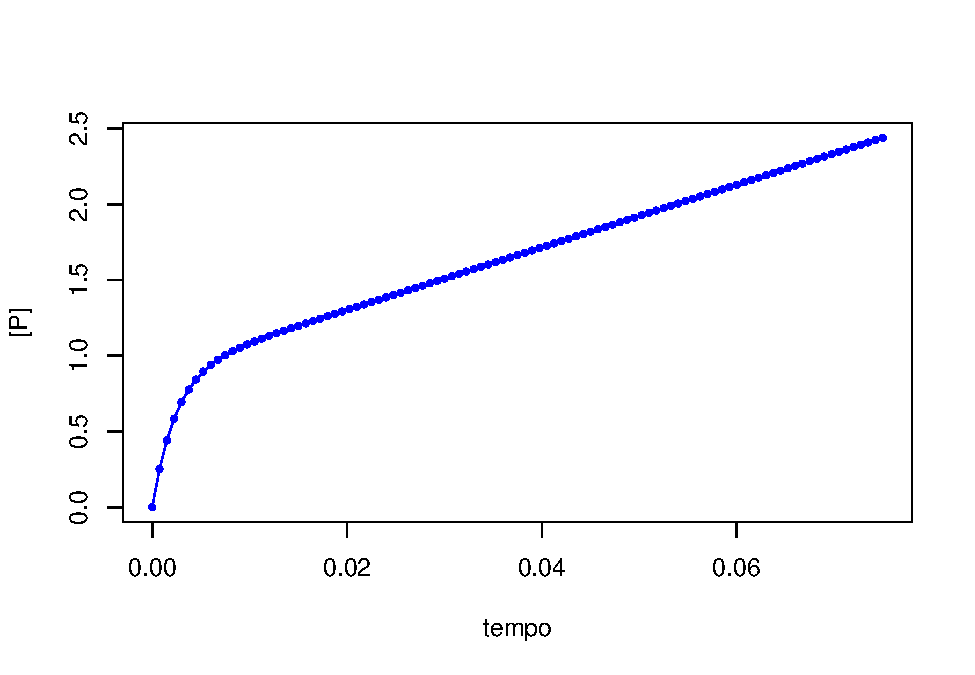
\includegraphics{Bioquímica-Quantitativa-com-R_files/figure-latex/figBurst-1.pdf}
\caption{\label{fig:figBurst}Formação de produto num modelo cinético de estado pré-estacionário.}
\end{figure}

~~~~~~Note pela figura \ref{fig:figBurst} que na cinética de estado transiente, existe uma fase pré-estacionária inicial eleva o teor de produto \emph{P} rapidamente, e que antecede a fase estacionária de liberação constante de \emph{P}.

~~~~~~Por outro lado, por vezes é necessário o oposto, ou seja, determinar as constantes de velocidade a partir do conhecimento dos parâmetros experimentais \emph{kobs} e \emph{Ao}. Nesse caso (e em tantos outros transdisciplinares) o \passthrough{\lstinline!R!} possui funções de minimização que permitem encontrar a raíz de equações lineares ou não lineares.\\
\hspace*{0.333em}\hspace*{0.333em}\hspace*{0.333em}\hspace*{0.333em}\hspace*{0.333em}\hspace*{0.333em}O procedimento envolve minimizar iterativamente um vetor de equações dadas as sementes para cada parâmetro. Para tal busca-se obter \emph{f(x) = 0} pela diferença entre um valor de referência; ou seja, quando a solução encontrar \emph{x} quando \emph{f(x)-y = 0}. Exemplificando, supondo que f(x) seja \emph{a+b/x}, e que y seja 3. Então a busca se dá no sentido de encontrar \emph{a} e \emph{b} em \emph{a+b/x-3}.\\
\hspace*{0.333em}\hspace*{0.333em}\hspace*{0.333em}\hspace*{0.333em}\hspace*{0.333em}\hspace*{0.333em}Para a determinação das constantes de velocidade representadas na cinética transiente, vale mencionar a função \passthrough{\lstinline!optim!} em \passthrough{\lstinline!stats!} ou o pacote \passthrough{\lstinline!rootSolve!}, que buscam minimizar equações lineares e não lineares para encontrar os valores de seus parâmetros.\\
\hspace*{0.333em}\hspace*{0.333em}\hspace*{0.333em}\hspace*{0.333em}\hspace*{0.333em}\hspace*{0.333em}Na solução dos parâmetros para estado pré-estacionário, ilustra-se abaixo o emprego do \passthrough{\lstinline!R!} com \passthrough{\lstinline!rootSolve!}, adicionando ainda a busca para \emph{Km} como segue.

\begin{equation}
Km = \frac{k3}{k2+k3} 
\label{eq:burstKm}
\end{equation}

\begin{lstlisting}[language=R]
# Cálculo de constantes cinéticas por solução de sistema de equações não lineares aplicadas à cinética de burst.

library(rootSolve) 
kobs =  0.06; Ao = 50; kcat = 300; Ks = 15
# define os parâmetros de ajuste não linear obtidos por curva progressiva experimental, t x P; 
# Obs: Ks obtido experimentalmente de curva de S x kobs

# Parâmetros
# x[1]=k2
# x[2]= k3
# x[3] = Km

# Modelo
model = function(x) c(x[1]/kobs^2-Ao,(x[1]*x[2])/kobs-kcat,Ks*x[2]/(x[1]+x[2])-x[3])
# o modelo acima deve conter uma lista de equações cuja igualdade é zero, ou seja, f(x)=0
(ss=multiroot(model,c(1,1,1))) # comando de execução do rootSolve (sementes pro algoritmo)
\end{lstlisting}

\begin{lstlisting}
## $root
## [1]   0.2 100.0  15.0
## 
## $f.root
## [1]  0e+00  1e-13 -1e-09
## 
## $iter
## [1] 4
## 
## $estim.precis
## [1] 4e-10
\end{lstlisting}

~~~~~~Os resultados da minimização podem ser interpretados como:

\begin{enumerate}
\def\labelenumi{\arabic{enumi}.}
\tightlist
\item
  \emph{root} = valores de xi pra f(xi)=0 ; ou seja, \emph{k2, k3, e Km};
\item
  \emph{f.root} = valor de cada função pra cada xi (deve ser próximo de zero para cada);
\item
  \emph{iter} = no. iterações ;
\item
  \emph{esti.precis} = estimativa da precisão.
\end{enumerate}

~~~~~~A contemplar um capítulo ainda que extenso sobre cinética enzimática, existem inúmeros tópicos deixados de lado, dado o foco principal do emprego do \passthrough{\lstinline!R!} na solução de problemas quantitativos em biofísico-química. Dessa forma, omitimos diversos conceitos, tais como \emph{cinética lenta de interação de substrato (slow binding), cinética de múltiplos substratos (reação sequencial e ping-pong), equação integrada de Michaelis-Menten e curvas progressivas, ativação de moduladores, influência de pH e temperatura na catálise, e enzimas multisítios}, entre vários.

\hypertarget{Binding}{%
\chapter{Interação Biomolecular}\label{Binding}}

~~~~~~Quando se menciona interação entre biomoléculas, normalmente se faz referência à processos adsortivos envolvendo um biopolímero (proteína, ácido nucleico, glicano), e um ligante de baixo peso molecular, embora o formalismo também se aplique com alguma restrição a interações entre biopolímeros, e mesmo células inteiras.\\
\hspace*{0.333em}\hspace*{0.333em}\hspace*{0.333em}\hspace*{0.333em}\hspace*{0.333em}\hspace*{0.333em}O formalismo mais comum para interação biomolecular é o que envolve a formação de complexo adsortivo entre uma proteína e um ligante (\emph{ligand binding}), exemplificado para íons (Ca\(^{2+}\), Mg\(^{2+}\), etc), fármacos e candidatos, produtos naturais, e antígenos, dentre vários.\\
\hspace*{0.333em}\hspace*{0.333em}\hspace*{0.333em}\hspace*{0.333em}\hspace*{0.333em}\hspace*{0.333em}Perguntas simples acerca da \emph{interação ligante-proteína} podem elucidar diversas características da formação de tais complexos, como:

\begin{enumerate}
\def\labelenumi{\arabic{enumi}.}
\tightlist
\item
  Quanto de proteína/ligante estão presentes ?
\item
  Quanto do complexo é formado ?
\item
  Quão rápido o complexo associa/dissocia ?
\item
  Quais os mecanismos envolvidos ?
\end{enumerate}

~~~~~~De modo geral, pode-se representar a interação ligante-proteína como segue:

\begin{equation}
P+L \begin{array}{c}
_{k_{on}}\\
 \rightleftharpoons\\
^{k_{off}} \end{array} PL 
 \label{eq:diagPL}
\end{equation}

Onde \emph{P} representa o teor de proteína livre, \emph{L} o ligante livre, e \emph{PL} o complexo formado. As taxas de reação são definidas para a formação (\emph{k\(_{on}\)}; M\(^{-1}\)s\(^{-1}\)) e dissociação (\emph{k\(_{off}\)}; s\(^{-1}\)) do complexo.

~~~~~~Dessa forma deduz-se a equação para a \emph{isoterma de interação} do ligante com a proteína como segue:

\begin{equation}
Kd=\frac{[P]*[L]}{[P]+[L]}
\label{eq:eqPL}
\end{equation}

Onde \emph{Kd} representa a \emph{constante de equilíbrio de dissociação} para o complexo \emph{PL} formado, tal como condicionado ao equilíbrio de formação/dissociação do complexo (\emph{v\(_{assoc}\) = v\(_{dissoc}\)}), e também definido como:

\begin{equation}
Kd=\frac{k_{off}}{k_{on}}
\label{eq:eqKd}
\end{equation}

~~~~~~A partir da Eq. \eqref{eq:eqPL} pode-se facilmente deduzir a expressão final para a interação de um ligante a um conjunto de sítios de mesma afinidade na proteína:

\begin{equation}
\nu=\frac{n * [L]}{Kd + [L]}
\label{eq:eqNu}
\end{equation}

\hypertarget{modelos-de-interauxe7uxe3o-e-representauxe7uxf5es-lineares}{%
\section{Modelos de Interação e Representações Lineares}\label{modelos-de-interauxe7uxe3o-e-representauxe7uxf5es-lineares}}

~~~~~~Observe que a equação \eqref{eq:eqNu} praticamente repete o formalismo já visto com a formação do complexo ativado de enzima-substrato \eqref{eq:eqMM}, bem como sua representação resultante como uma hipérbole quadrática. De fato, ocorre essencialmente a substituição do parâmetro cinético \emph{v} da reação pelo parâmetro termodinâmico \(\nu\) (``nu'', do Grego) para a isoterma de ligação. As demais quantidades envolvidas mantém-se análogas (\emph{P} no lugar de \emph{E}; \emph{L} no lugar de \emph{S};\emph{Kd} no lugar de \emph{Km}; e \emph{n} no lugar de \emph{Vmax}).\\
\hspace*{0.333em}\hspace*{0.333em}\hspace*{0.333em}\hspace*{0.333em}\hspace*{0.333em}\hspace*{0.333em}Mantida essa similaridade com o formalismo da \emph{equação de Michaelis-Menten}, da mesma maneira decorrem as linearizações para a Eq. \eqref{eq:eqNu}, bem como ajustes não lineares à mesma, na busca de uma \emph{solução analítica} para os parâmetros termodinâmicos \emph{Kd} e \emph{n}. Exemplificando um trecho de código para as linearizações mais comuns no tratamento de dados de interação ligante-proteína:

\begin{lstlisting}[language=R]
L=c(0.1,0.2,0.5,1,5,10,20)*1e-6
Kd=1e-6;n=1
v=n*L/(Kd+L)
par(mfrow=c(2,3)) # estabelece área de plot pra 6 gráficos
plot(L,v,type="o",main="Direto")
plot(log(L),v,type="o",main="Langmuir")
plot(1/L,1/v,type="o",main="Klotz")
plot(v,v/L,type="o",main="Scatchard")
plot(L,L/v,type="o",main="Woolf")
plot(log10(L),log10(v/(n-v)),type="o",main="Hill") 
\end{lstlisting}

\begin{figure}
\centering
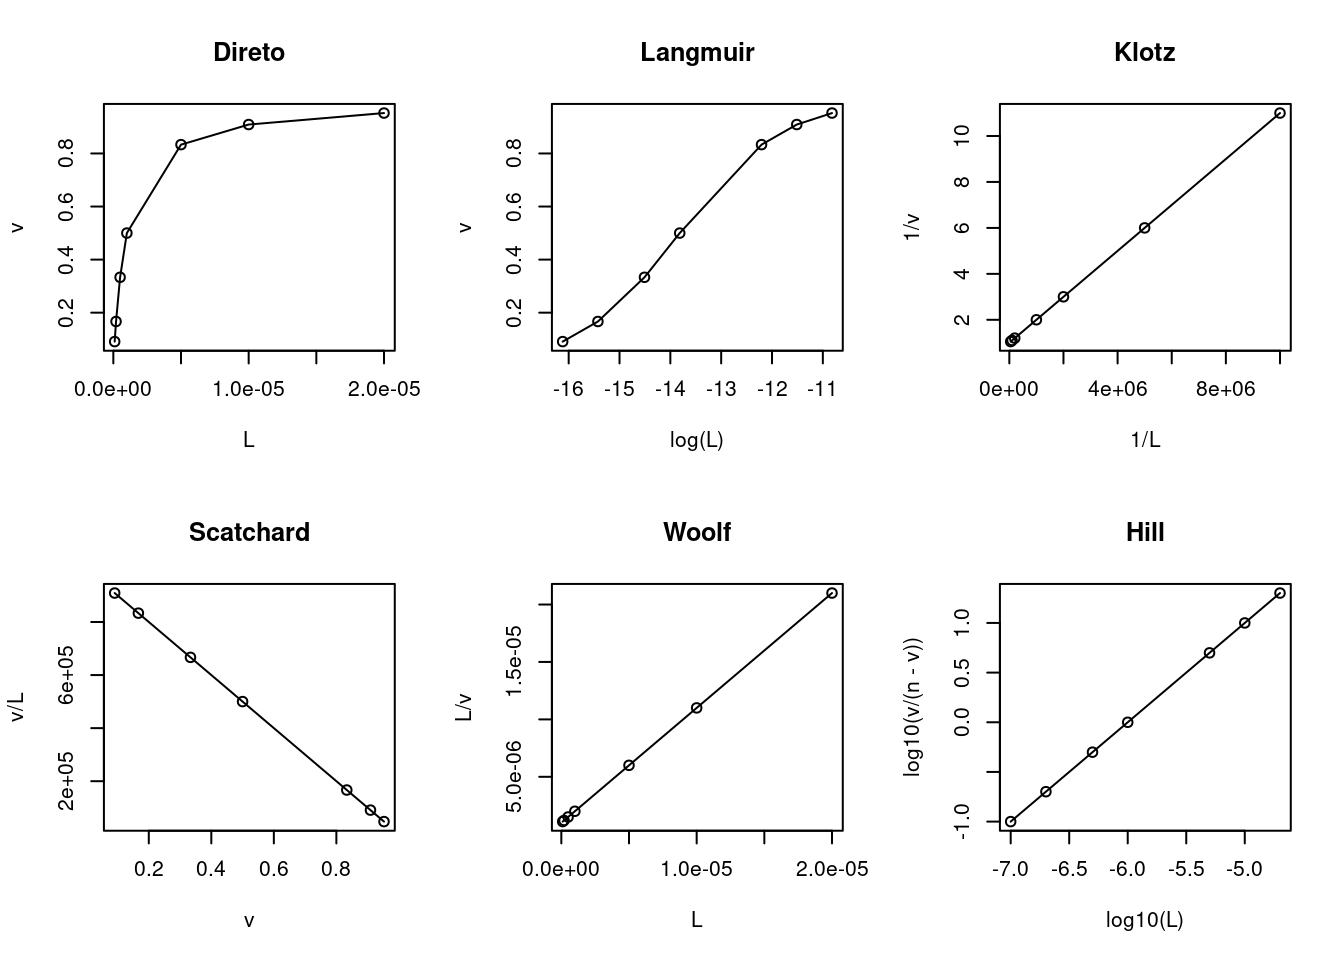
\includegraphics{Bioquímica-Quantitativa-com-R_files/figure-latex/figLinBind-1.pdf}
\caption{\label{fig:figLinBind}Principais linearizações da isoterma de ligação ligante-proteína.}
\end{figure}

\begin{lstlisting}[language=R]
par(mfrow=c(1,1)) # volta à janela gráfica normal
\end{lstlisting}

~~~~~~Desvios da linearidade, por outro lado, são frequentemente utilizados como diagnósticos para modelos que distintos do de \emph{homogeneidade de sítios de ligação} como acima (\emph{heterogeneidade de sítios}, \emph{criação de sítio}, \emph{cooperatividade}. As equações abaixo descrevem esses modelos, e consideram \emph{K}, \emph{constante de equilíbrio de associação ligante-proteína}, como o reverso de \emph{Kd}, a fim de tornar as expressões mais legíveis:

\begin{equation}
K = \frac{1}{Kd}
\label{eq:eqKdK}
\end{equation}

~~~~~~O \emph{modelo de heterogeneidade de sítios} de ligação pressupõe que haja na proteína mais um sítio com afinidades distintas para o ligante (\citep{dahlquist197813}). Formalmente esse modelo pode ser exemplificado para 2 conjuntos de sítios de ligação, como segue:

\begin{equation}
\nu=\frac{K1*[L]}{1+K1*[L]} + \frac{K2*[L]}{1+K2*[L]}
\label{eq:eqHeterSit}
\end{equation}

~~~~~~O trecho de código abaixo exemplifica o modelo no `R', bem como suas principais linearizações diagnósticas.

\begin{lstlisting}[language=R]
L=c(0.1,0.2,0.5,1,5,10,20)*1e-6
Kd1=2e-6;n1=1;
Kd2=2e-8;n2=1
v=(n1*L/(Kd1+L))+(n2*L/(Kd2+L))

par(mfrow=c(2,3)) # estabelece área de plot pra 6 gráficos
plot(L,v,type="o",main="Direto")
plot(log(L),v,type="o",main="Langmuir")
plot(1/L,1/v,type="o",main="Klotz")
plot(v,v/L,type="o",main="Scatchard")
plot(L,L/v,type="o",main="Woolf")
plot(log10(L),log10(v/(n1+n2-v)),type="o",main="Hill") # n1+n2=ntot no Hill
\end{lstlisting}

\begin{figure}
\centering
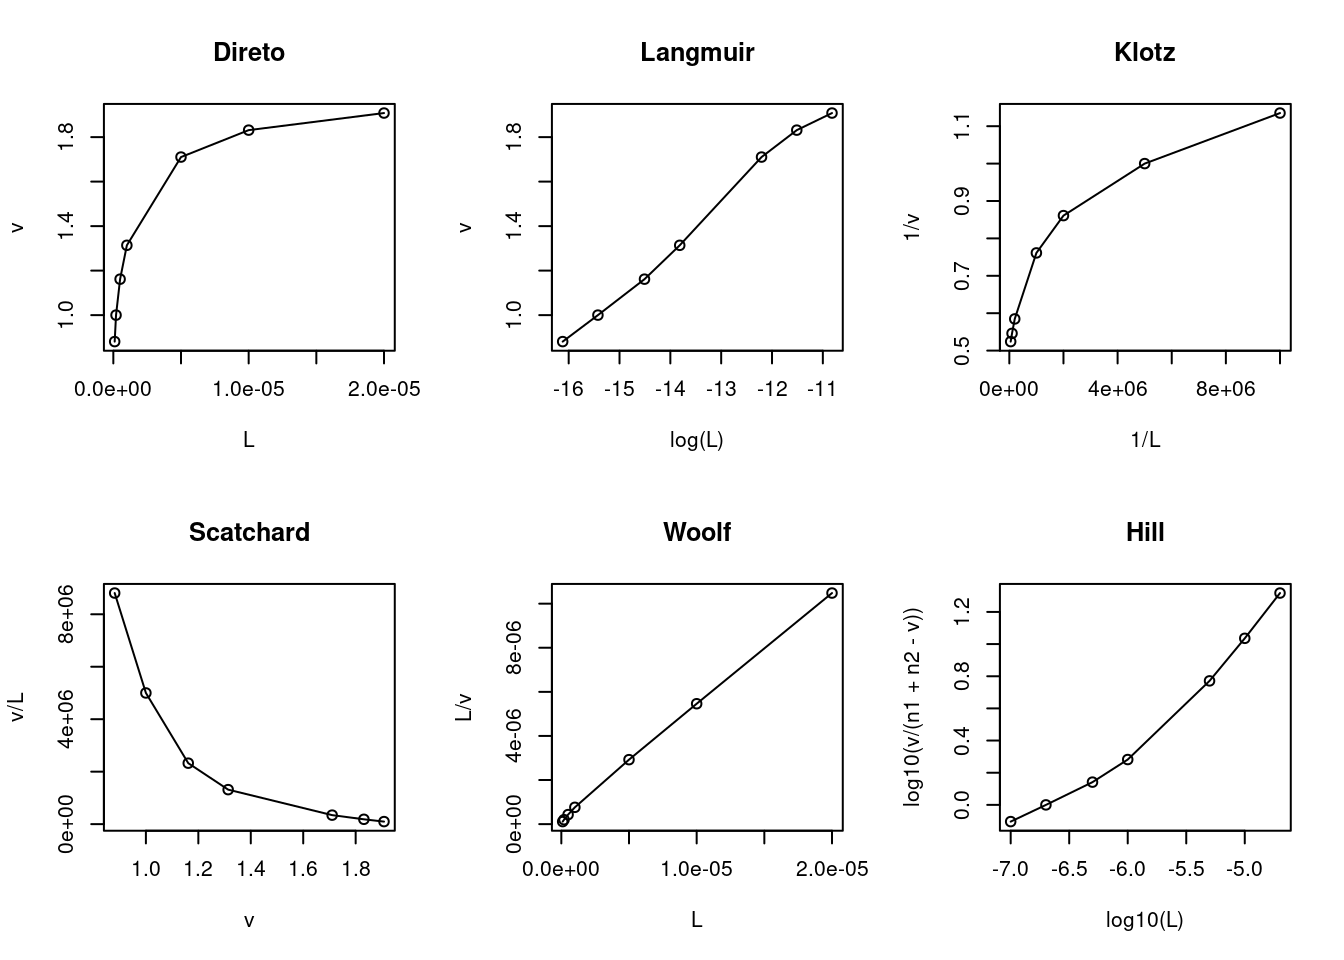
\includegraphics{Bioquímica-Quantitativa-com-R_files/figure-latex/figHeterSit-1.pdf}
\caption{\label{fig:figHeterSit}Modelo e linearizações para heterogeneidade de 2 conjuntos de sítios de ligação}
\end{figure}

\begin{lstlisting}[language=R]
par(mfrow=c(1,1)) # volta à janela gráfica normal
\end{lstlisting}

~~~~~~O \emph{modelo de criação de novo sítio} - ``one-site creator''; \citep{parsons1978theoretical} estabelece uma cooperatividade positiva resultante da produção de novos sítios para o ligante na proteína. Segue o modelo exemplificado e suas linearizações resultantes.

\begin{lstlisting}[language=R]
L=c(0.1,0.2,0.5,1,5,10,20)*1e-6
Kd1=2e-6;n1=1
Kd2=2e-5;n2=1
nH=0.5
v=(n1*L*1/Kd1)/(1+1/Kd1*L)+((n2*1/Kd1*1/Kd2*L^2)/(1+1/Kd1*L)*(1+1/Kd2*L))
par(mfrow=c(2,3)) # estabelece área de plot pra 6 gráficos
plot(L,v,type="o",main="Direto")
plot(log(L),v,type="o",main="Langmuir")
plot(1/L,1/v,type="o",main="Klotz")
plot(v,v/L,type="o",main="Scatchard")
plot(L,L/v,type="o",main="Woolf")
plot(log10(L),log10(v/(n-v)),type="o",main="Hill") # n1+n2=ntot no Hill
\end{lstlisting}

\begin{lstlisting}
## Warning in xy.coords(x, y, xlabel, ylabel, log): NaNs produced
\end{lstlisting}

\begin{figure}
\centering
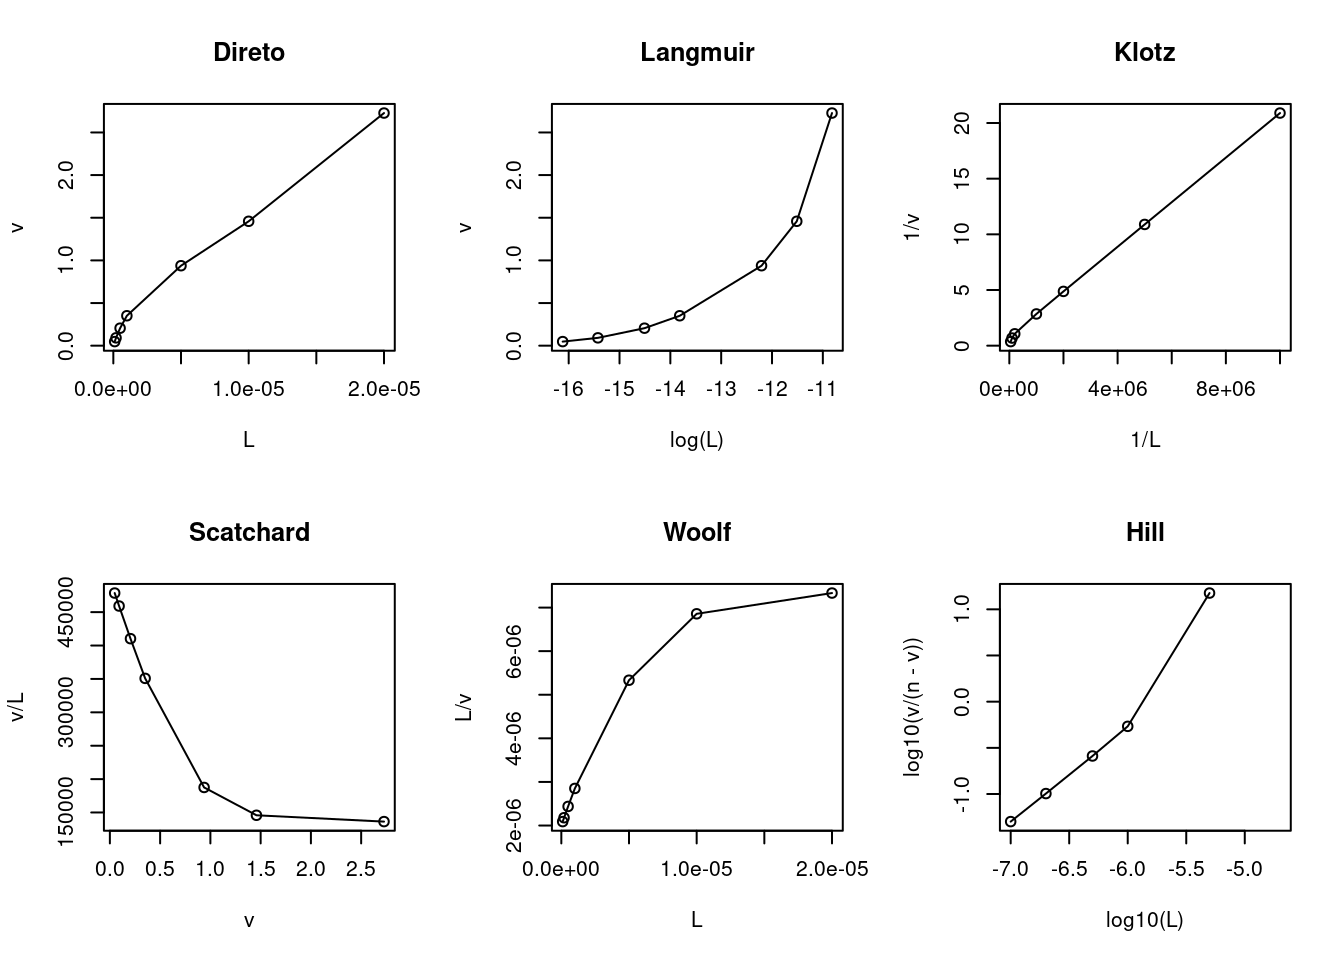
\includegraphics{Bioquímica-Quantitativa-com-R_files/figure-latex/figOneSitCreat-1.pdf}
\caption{\label{fig:figOneSitCreat}Modelo e linearizações para criação de novo sítio: \emph{1-site creator}.}
\end{figure}

\begin{lstlisting}[language=R]
par(mfrow=c(1,1)) # volta à janela gráfica normal
\end{lstlisting}

~~~~~~Os \emph{modelos de cooperatividade (negativa e positiva)} seguem um formalismo similar descrito para a ligação de oxigênio à hemoglobina junto ao capítulo \ref{Proteinas} (Eq. \eqref{eq:Hb}). Na \emph{cooperatividade negativa} uma segunda molécula de ligante interage com a proteína com menor afinidade:

\begin{lstlisting}[language=R]
L=c(0.1,0.2,0.5,1,5,10,20)*1e-6
Kd=2e-6;n=1
nH=0.5
v=(n*L^nH/(Kd+L^nH))
par(mfrow=c(2,3)) # estabelece área de plot pra 6 gráficos
plot(L,v,type="o",main="Direto")
plot(log(L),v,type="o",main="Langmuir")
plot(1/L,1/v,type="o",main="Klotz")
plot(v,v/L,type="o",main="Scatchard")
plot(L,L/v,type="o",main="Woolf")
plot(log10(L),log10(v/(n-v)),type="o",main="Hill") # n1+n2=ntot no Hill
\end{lstlisting}

\begin{figure}
\centering
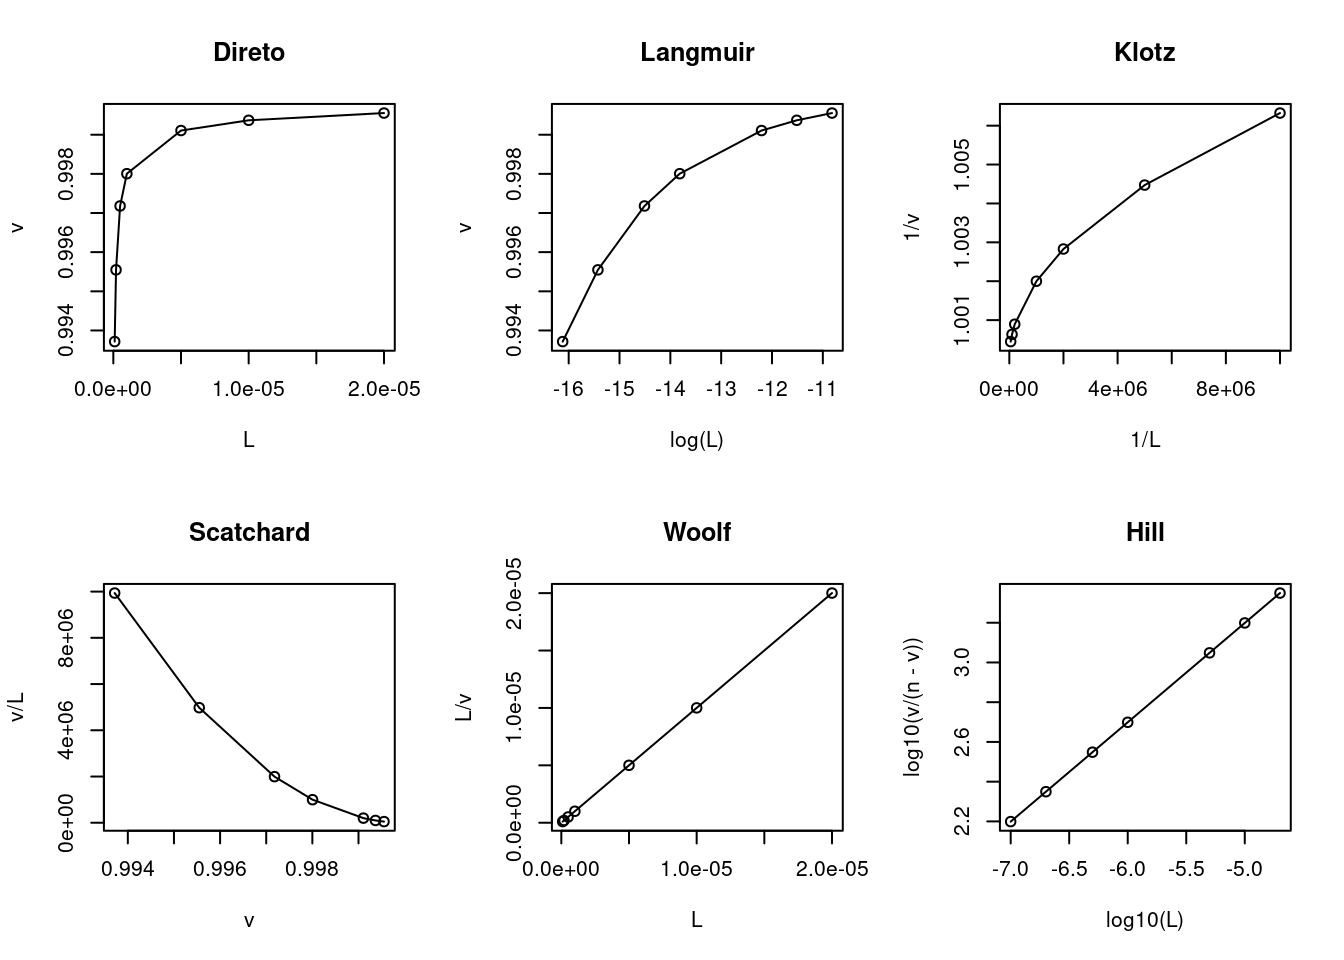
\includegraphics{Bioquímica-Quantitativa-com-R_files/figure-latex/figCoopNeg-1.pdf}
\caption{\label{fig:figCoopNeg}Modelo e linearizações para cooperatividade negativa de sítios de ligação.}
\end{figure}

\begin{lstlisting}[language=R]
par(mfrow=c(1,1)) # volta à janela gráfica normal
\end{lstlisting}

~~~~~~Já na \emph{cooperatividade positiva}, uma segunda molécula de ligante interage com a proteína com maior afinidade que a primeira molécula \citep{parsons1978theoretical}:

\begin{lstlisting}[language=R]
L=c(0.1,0.2,0.5,1,5,10,20)*1e-6
Kd=2e-6;n=1
nH=1.5
v=(n*L^nH/(Kd+L^nH))
par(mfrow=c(2,3)) # estabelece área de plot pra 6 gráficos
plot(L,v,type="o",main="Direto")
plot(log(L),v,type="o",main="Langmuir")
plot(1/L,1/v,type="o",main="Klotz")
plot(v,v/L,type="o",main="Scatchard")
plot(L,L/v,type="o",main="Woolf")
plot(log10(L),log10(v/(n-v)),type="o",main="Hill") # n1+n2=ntot no Hill
\end{lstlisting}

\begin{figure}
\centering
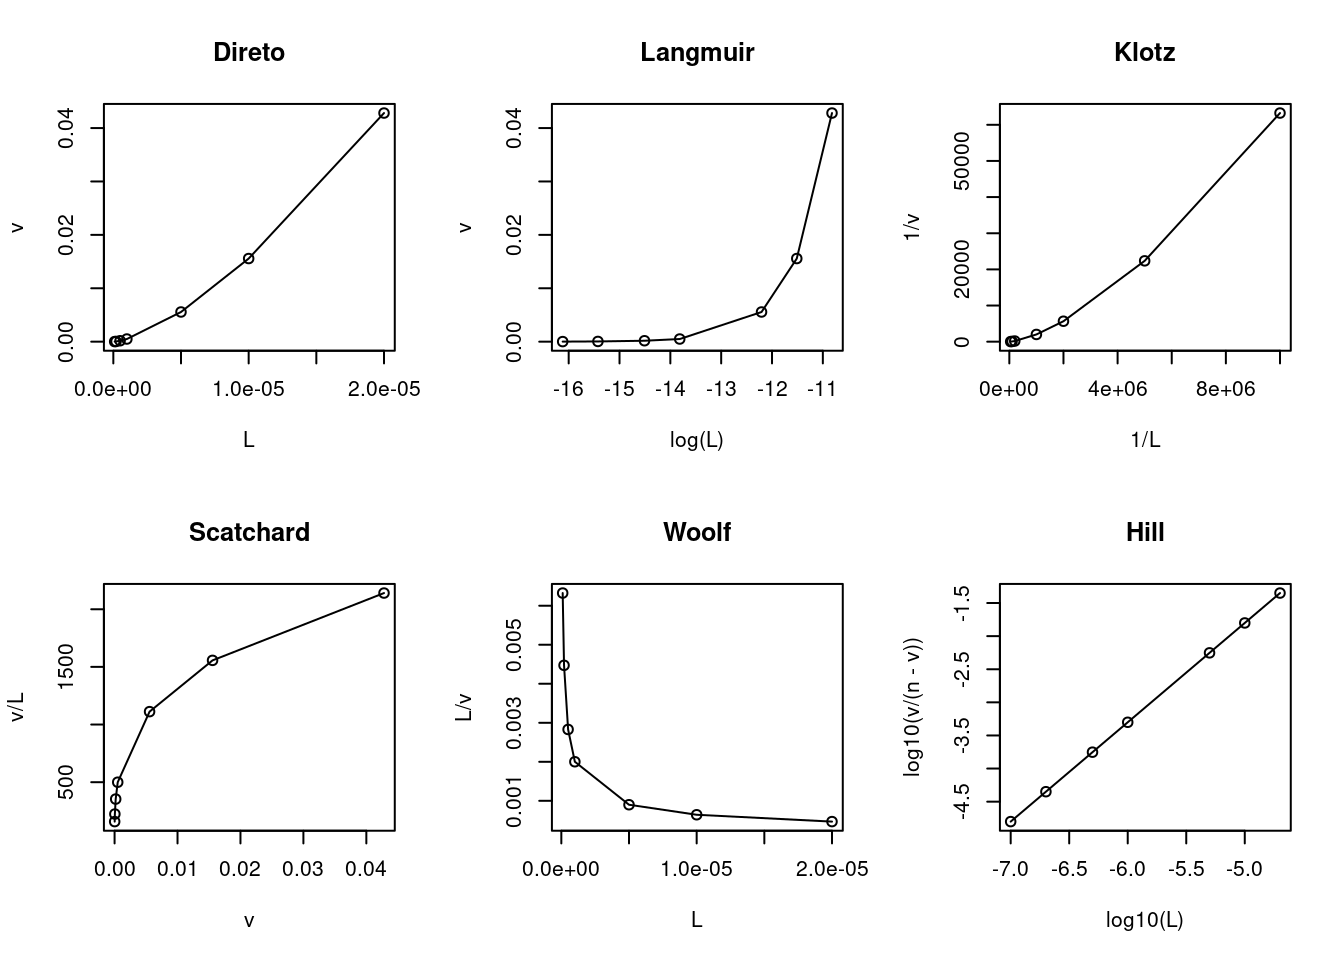
\includegraphics{Bioquímica-Quantitativa-com-R_files/figure-latex/figCoopPos-1.pdf}
\caption{\label{fig:figCoopPos}Modelo e linearizações para cooperatividade positiva de sítios de ligação.}
\end{figure}

\begin{lstlisting}[language=R]
par(mfrow=c(1,1)) # volta à janela gráfica normal
\end{lstlisting}

~~~~~~Observe que a inclinação do gráfico de \emph{Hill} é inferior à unidade para a \emph{cooperatividade negativa}, e superior a essa, para a \emph{cooperatividade positiva}, e representa o mesmo parâmetro \emph{nH} visto na Eq.\eqref{eq:Hb}.\\
\hspace*{0.333em}\hspace*{0.333em}\hspace*{0.333em}\hspace*{0.333em}\hspace*{0.333em}\hspace*{0.333em}Ainda que sujeito à crítica por sua inconsistência estatística (variável dependente em ambos os eixos), a representação de Scatchard tem sido privilegiada ao longo de décadas como diagnóstico de modelos de interação ligante-proteína. Entre suas vantagens, aloca-se a possibilidade de facilmente distinguir-se o modelo de cooperatividade positiva (aclive) do de heterogeneidade de sítios de ligação (declive abrupto) ou de cooperatividade negativa (declive suave).

\hypertarget{ajuste-nuxe3o-linear-em-interauxe7uxe3o-ligante-proteuxedna}{%
\section{Ajuste Não-Linear Em Interação Ligante-Proteína}\label{ajuste-nuxe3o-linear-em-interauxe7uxe3o-ligante-proteuxedna}}

~~~~~~Ajustes diretos da equação não linear dos modelos de interação também podem ser efetuados como fora realizado para a equação de Michaelis-Menten no capítulo \ref{Enzimas} sobre Enzimas. Exemplificando, pode-se simular a obtenção de dados experimentais de \emph{binding} pelo trecho a seguir, utilizando-se o comando `runif' (\emph{random uniform}) para geração de sequência aleatória (como fora realizado no capítulo \ref{Enzimas}.

\begin{lstlisting}[language=R]
# Isoterma de Interação Ligante-Proteína
n=1
Kd=10
L=120
i=3
L=seq(0, L, i)
v=(L*n)/(Kd+L)+rnorm(40,0,0.1)
\end{lstlisting}

\begin{lstlisting}
## Warning in (L * n)/(Kd + L) + rnorm(40, 0, 0.1): longer object length is not a
## multiple of shorter object length
\end{lstlisting}

\begin{lstlisting}[language=R]
plot(L,v)
\end{lstlisting}

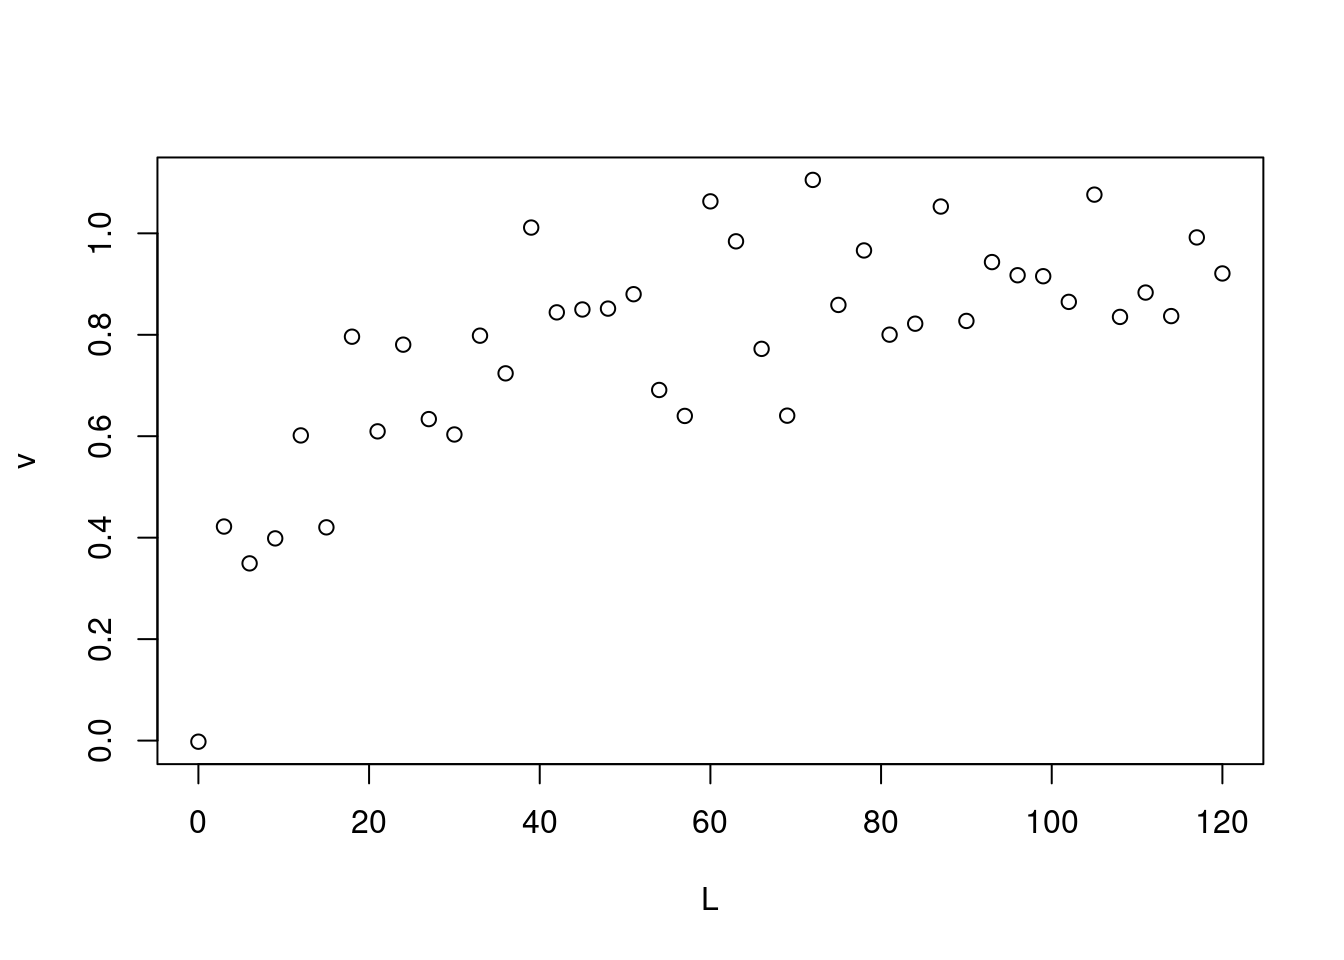
\includegraphics{Bioquímica-Quantitativa-com-R_files/figure-latex/1SitBindSimul-1.pdf}

~~~~~~Observe que o comando `rnorm' adiciona um erro de distribuição normal aos dados. Outra forma para simulação desses é dada abaixo, introduzindo-se o comando `runif' de geração de números aleatórios.

\begin{lstlisting}[language=R]
# Simulação de dados de interação bimolecular (1 sítio)

# Simulação de dados
set.seed(20160227) # estabelece semente para geração de números aleatórios
L<-seq(0,50,1)
PL<-((runif(1,10,20)*L)/(runif(1,0,10)+L))+rnorm(51,0,1) 
# 1. runif(n,min,max); quando sem atributos, considera-se min=0  e max=1
# 2. rnorm(no. pontos,media,desvio) - erro aleatório de distribuição normal
plot(L,PL, xlab="L", ylab="PL")
\end{lstlisting}

\begin{figure}
\centering
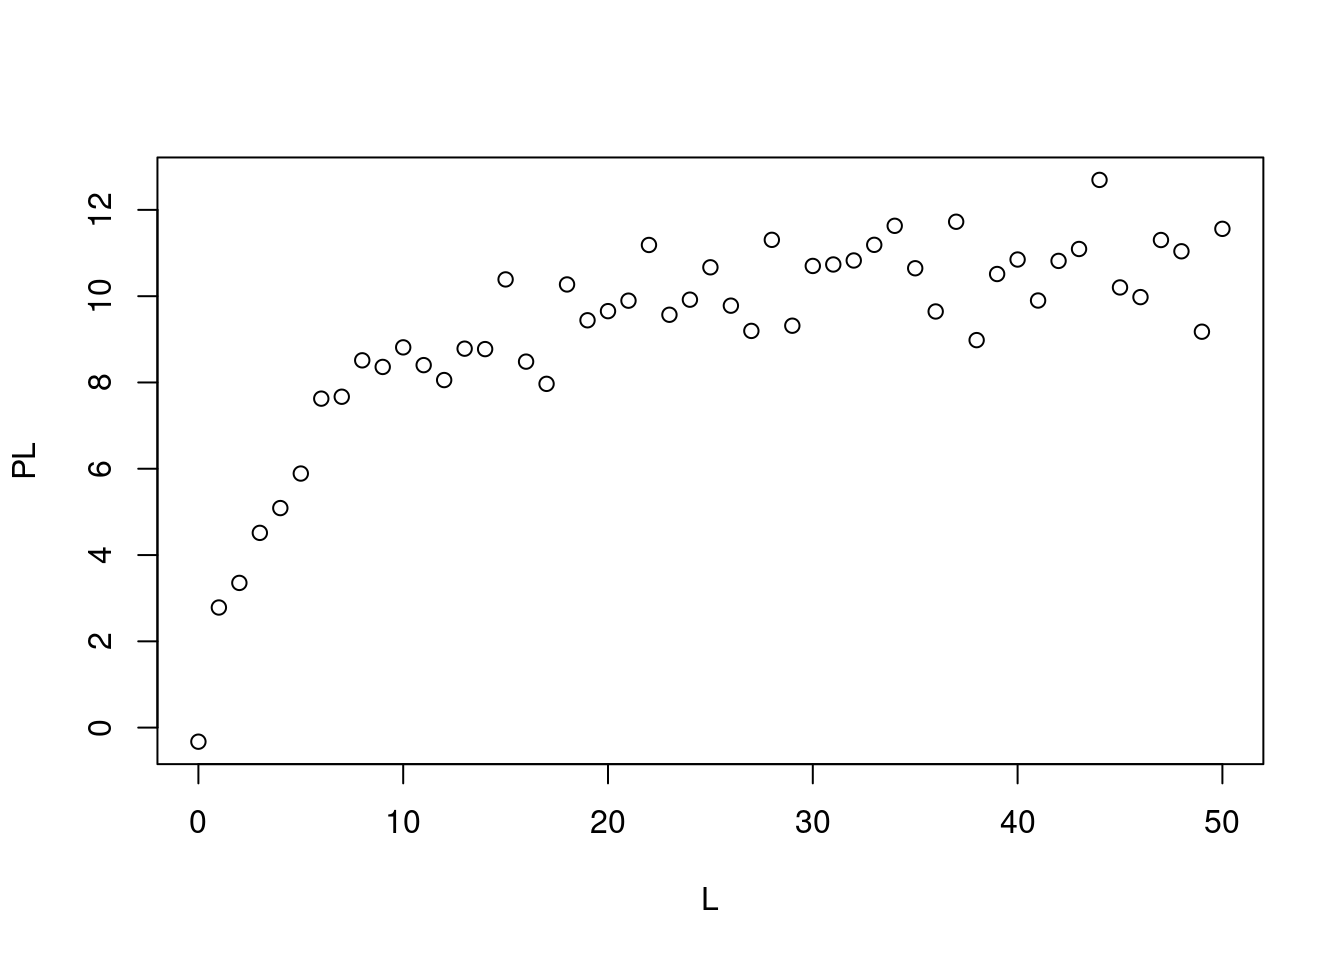
\includegraphics{Bioquímica-Quantitativa-com-R_files/figure-latex/1sitBindSimul2-1.pdf}
\caption{\label{fig:1sitBindSimul2}Dados simulados para isoterma de interação bimolecular.}
\end{figure}

~~~~~~Agora precisamos utilizar o comando `nls' para o ajuste não linear, sobreposição da curva teórica, e tabela estatística de resultados:

\begin{lstlisting}[language=R]
#Ajuste não linear
m<-nls(PL~n*L/(Kd+L),start=list(n=1,Kd=1))

#Coef. de correlação
cor(PL,predict(m)) # Coeficiente de correlação de Pearson
\end{lstlisting}

\begin{lstlisting}
## [1] 0.9
\end{lstlisting}

\begin{lstlisting}[language=R]
#Gráfico de dados e simulação
plot(L,PL)
lines(L,predict(m),lty=2,col="red",lwd=3)
\end{lstlisting}

\includegraphics{Bioquímica-Quantitativa-com-R_files/figure-latex/nlsBind-1.pdf}

\begin{lstlisting}[language=R]
summary(m)
\end{lstlisting}

\begin{lstlisting}
## 
## Formula: PL ~ n * L/(Kd + L)
## 
## Parameters:
##    Estimate Std. Error t value Pr(>|t|)    
## n    11.848      0.262   45.22  < 2e-16 ***
## Kd    4.278      0.511    8.37  5.3e-11 ***
## ---
## Signif. codes:  0 '***' 0.001 '**' 0.01 '*' 0.05 '.' 0.1 ' ' 1
## 
## Residual standard error: 0.8 on 49 degrees of freedom
## 
## Number of iterations to convergence: 6 
## Achieved convergence tolerance: 1.56e-06
\end{lstlisting}

\hypertarget{sistemas-gruxe1ficos-no-r}{%
\section{Sistemas Gráficos no R}\label{sistemas-gruxe1ficos-no-r}}

~~~~~~A última curva de simulação obtida o foi junto à biblioteca padrão para manipulação de gráficos da instalação do `R', \textbf{Graphics}. Trata-se um conjunto de funções amplo também utilizado por vários outros pacotes do ambiente. Contudo, existem no `R' diversas outras bibliotecas para elaboração de gráficos, dentre os quais vale destacar o \emph{Lattice}, também incluido na instalação padrão, e o \emph{ggplot2}. Ambos os sistemas geram resultados com melhor estética e flexibilidade gráfica que a biblioteca \emph{Graphics} padrão, e possuem empregos e semânticas distintas entre si.\\
\hspace*{0.333em}\hspace*{0.333em}\hspace*{0.333em}\hspace*{0.333em}\hspace*{0.333em}\hspace*{0.333em}O sistema \emph{Lattice} \citep{sarkar2008lattice} é baseado no sistema \emph{Trellis} para representação gráfica de dados multivariados. Sua força está na representação de dados em paineis contendo subgrupos e, embora tenha sintaxe menos intuitiva e por vezes mais elaborada que o pacote \emph{Graphics}, produz um grafismo superior a esse com poucos cliques de teclado. De modo geral, o \emph{Lattice} produz o gráfico dentro do próprio algoritmo, de modo diferente aos sistemas \emph{Graphics} (pode-se acumular linhas sucessivas de modificação do gráfico) ou \emph{ggplot2}.\\
\hspace*{0.333em}\hspace*{0.333em}\hspace*{0.333em}\hspace*{0.333em}\hspace*{0.333em}Por outro lado a biblioteca \emph{ggplot2} é baseada na gramática de gráficos \citep{wickham2011ggplot2}, e produz o gráfico utilizando uma única linha de comando que combina camadas sobrepostas, de modo similar à aplicativos de manipulação de imagens (ex: \emph{Inkscape}, \emph{Gimp}, \emph{Corel Draw}, \emph{Photoshop}). Dessa forma é possível alterar cada ítem do gráfico em suas camadas específicas (tema, coordenadas, facets, estatísticas, geometria, estética, dados). Exemplificando o resultado gráfico da curva de simulação acima de \emph{binding} para \emph{Lattice} e \emph{ggplot2}:

\begin{lstlisting}[language=R]
# Simulação de dados
set.seed(20160227) # estabelece semente para geração de números aleatórios
L<-seq(0,50,1)
PL<-((runif(1,10,20)*L)/(runif(1,0,10)+L))+rnorm(51,0,1) 
# 1. runif(n,min,max); quando sem atributos, considera-se min=0  e max=1
# 2. rnorm(no. pontos,media,desvio) - erro aleatório de distribuição normal

# Produção do gráfico com sistema Lattice
library(lattice)
xyplot(PL~L)
\end{lstlisting}

\includegraphics{Bioquímica-Quantitativa-com-R_files/figure-latex/1sitBindSimulLattice-1.pdf}

\begin{lstlisting}[language=R]
# Produção do gráfico com sistema ggplot2
library(ggplot2)
qplot(L,PL)
\end{lstlisting}

\includegraphics{Bioquímica-Quantitativa-com-R_files/figure-latex/1sitBindSimulLattice-2.pdf}

~~~~~~Como a percepção de peculiaridades dos sistemas gráficos se revela melhor com dados mais elaborados, as ilustrações a seguir utilizarão o conjunto de dados `Puromycin', que integra a biblioteca `datasets' do `R'. Os dados apresentam a velocidade de reação enzimática sobre um substrato em células tratadas e não tratadas com puromicina.

~~~~~~O código abaixo retorna a plotagem, ajuste não linear e resultados obtidos com a biblioteca \emph{Graphics} padrão, e foi extraído do própria documentação do \emph{dataset}.

\begin{lstlisting}[language=R]
library(datasets)

plot(rate ~ conc, data = Puromycin, las = 1,
     xlab = "[S], mM",
     ylab = "v (contagem/min/min)",
     pch = as.integer(Puromycin$state),
     col = as.integer(Puromycin$state),
     main = "Ilustração de Ajuste Com Graphics")

## Ajuste da equação de Michaelis-Mentem
fm1 <- nls(rate ~ Vm * conc/(K + conc), data = Puromycin,
           subset = state == "treated",
           start = c(Vm = 200, K = 0.05))
fm2 <- nls(rate ~ Vm * conc/(K + conc), data = Puromycin,
           subset = state == "untreated",
           start = c(Vm = 160, K = 0.05))
summary(fm1)
\end{lstlisting}

\begin{lstlisting}
## 
## Formula: rate ~ Vm * conc/(K + conc)
## 
## Parameters:
##    Estimate Std. Error t value Pr(>|t|)    
## Vm 2.13e+02   6.95e+00   30.61  3.2e-11 ***
## K  6.41e-02   8.28e-03    7.74  1.6e-05 ***
## ---
## Signif. codes:  0 '***' 0.001 '**' 0.01 '*' 0.05 '.' 0.1 ' ' 1
## 
## Residual standard error: 11 on 10 degrees of freedom
## 
## Number of iterations to convergence: 5 
## Achieved convergence tolerance: 8.82e-06
\end{lstlisting}

\begin{lstlisting}[language=R]
summary(fm2)
\end{lstlisting}

\begin{lstlisting}
## 
## Formula: rate ~ Vm * conc/(K + conc)
## 
## Parameters:
##    Estimate Std. Error t value Pr(>|t|)    
## Vm 1.60e+02   6.48e+00   24.73  1.4e-09 ***
## K  4.77e-02   7.78e-03    6.13  0.00017 ***
## ---
## Signif. codes:  0 '***' 0.001 '**' 0.01 '*' 0.05 '.' 0.1 ' ' 1
## 
## Residual standard error: 10 on 9 degrees of freedom
## 
## Number of iterations to convergence: 5 
## Achieved convergence tolerance: 4.47e-06
\end{lstlisting}

\begin{lstlisting}[language=R]
## Adição de linhas de ajuste ao plot
conc <- seq(0, 1.2, length.out = 101)
lines(conc, predict(fm1, list(conc = conc)), lty = 1, col = 1)
lines(conc, predict(fm2, list(conc = conc)), lty = 2, col = 2)
legend(0.8, 120, levels(Puromycin$state),
       col = 1:2, lty = 1:2, pch = 1:2)
\end{lstlisting}

\begin{figure}
\centering
\includegraphics{Bioquímica-Quantitativa-com-R_files/figure-latex/puromycGraphics-1.pdf}
\caption{\label{fig:puromycGraphics}Plotagem e análise com graphics.}
\end{figure}

~~~~~~O sistema \emph{ggplot2}, por sua vez, exige que os comandos sejam elencados em camadas justapostas intercaladas com o sinal ``+'', como segue:

\begin{lstlisting}[language=R]
library(datasets)
p <- ggplot(data=Puromycin, aes(conc, rate, color = state)) +
  geom_point() +
  geom_smooth(
    method       = "nls",
    formula      = y ~ Vm*x/(Km+x),
    method.args  = list(start = list(Vm = 200, Km = 0.1)),
    se           = FALSE 
  ) # expressão que define o plot
p # variável que apresenta o plot
\end{lstlisting}

\begin{figure}
\centering
\includegraphics{Bioquímica-Quantitativa-com-R_files/figure-latex/puromycGgplot2-1.pdf}
\caption{\label{fig:puromycGgplot2}Plotagem e análise com ggplot2.}
\end{figure}

~~~~~~Perceba o menor número de instruções do \emph{script} para a produção do gráfico. Além disso, e diferente do \emph{Graphics}, \emph{ggplot2} permite adicionar camadas à linha de comandos principais, e apresentar os dados multivariados em paineis (funções `facet\_grid' e `facet\_wrap'), sem a necessidade de se utilizar o comando `mfrow' ou `mfcol' visto no capítulo, como segue:

\begin{lstlisting}[language=R]
p + facet_grid(rows = vars(state))
\end{lstlisting}

\begin{figure}
\centering
\includegraphics{Bioquímica-Quantitativa-com-R_files/figure-latex/puromycGgplot2Facet-1.pdf}
\caption{\label{fig:puromycGgplot2Facet}Plotagem e análise com ggplot2 - paineis (faceting).}
\end{figure}

~~~~~~\emph{Lattice} também possui uma economia de instruções em relação à \emph{Graphics}. Não considerando o ajuste estatístico, os grupos podem ser apresentados simplesmente utilizando-se a fórmula:

\begin{equation}
xyplot(y \sim x~|~ groups = z)
\label{eq:eqTrellis}
\end{equation}

\begin{lstlisting}[language=R]
library(lattice)
xyplot(rate ~ conc, data = Puromycin, groups=state)
\end{lstlisting}

\includegraphics{Bioquímica-Quantitativa-com-R_files/figure-latex/unnamed-chunk-48-1.pdf}

~~~~~~E para a representação dos ajustes não lineares:

\begin{lstlisting}[language=R]
library(nlme)
n1<-nlsList(rate ~ Vmax*conc/(Km+conc) | state, data=Puromycin, start=list(Vmax=200, Km=0.1))
summary(n1)
xyplot(rate ~ conc,groups = state, data =
         Puromycin) +
  layer(panel.curve(Vmax[1]*x/(Km[1]+x),col=1),
        data = as.list(coef(n1))) +
  layer(panel.curve(Vmax[2]*x/(Km[2]+x),col=2),
        data = as.list(coef(n1)))
\end{lstlisting}

~~~~~~A biblioteca \emph{Lattice} também permite a apresentação em paineis; diferente de \emph{ggplot2}, contudo, o gráfico é gerado algoritmicamente, sem a sobreposição de comandos:

\begin{lstlisting}[language=R]
library(nlme) # pacote quer permite regressão não linear com subgrupos
\end{lstlisting}

\begin{lstlisting}
## 
## Attaching package: 'nlme'
\end{lstlisting}

\begin{lstlisting}
## The following object is masked from 'package:dplyr':
## 
##     collapse
\end{lstlisting}

\begin{lstlisting}
## The following object is masked from 'package:seqinr':
## 
##     gls
\end{lstlisting}

\begin{lstlisting}[language=R]
nonlinLatt<-nlsList(rate~Vmax*conc/(Km+conc)| state, start=list(Vmax=200, Km=0.1), data=Puromycin)
summary(nonlinLatt)
\end{lstlisting}

\begin{lstlisting}
## Call:
##   Model: rate ~ Vmax * conc/(Km + conc) | state 
##    Data: Puromycin 
## 
## Coefficients:
##    Vmax 
##           Estimate Std. Error t value Pr(>|t|)
## treated        213          7      32    3e-11
## untreated      160          7      23    1e-09
##    Km 
##           Estimate Std. Error t value Pr(>|t|)
## treated       0.06      0.008       8    2e-05
## untreated     0.05      0.008       6    2e-04
## 
## Residual standard error: 10 on 19 degrees of freedom
\end{lstlisting}

\begin{lstlisting}[language=R]
xyplot(rate + fitted(nonlinLatt)~conc| state, data=Puromycin,
       type=c("p","l"),distribute.type=TRUE,col.line="red",
       ylab="rate")
\end{lstlisting}

\begin{figure}
\centering
\includegraphics{Bioquímica-Quantitativa-com-R_files/figure-latex/puromicLatticePan-1.pdf}
\caption{\label{fig:puromicLatticePan}Plotagem e análise com Lattice - ajuste externo e paineis.}
\end{figure}

~~~~~~Das muitas diferenças que os pacotes \emph{ggplot2} e \emph{Lattice} apresentam, há uma que vale a pena ressaltar. Como visto acima, o \emph{ggplot2} realiza o ajuste não linear dentro da linha de comandos de geração do gráfico, ao passo que o \emph{Lattice} permite fazê-lo fora da linha. Isso é inerente do \emph{ggplot2}, uma biblioteca desenhada para a produção de gráficos, e não para análises computacionais. Dessa forma o algoritmo que permite o ajuste não linear pelo \emph{ggplot2}, ainda que seja o mesmo `nls' já trabalhado, não expressa seus resultados explicitamente (embora haja formas de ``pescá-los'' utilizando-se outros pacotes).\\
\hspace*{0.333em}\hspace*{0.333em}\hspace*{0.333em}\hspace*{0.333em}\hspace*{0.333em}\hspace*{0.333em}De certa forma, ainda que o \emph{Lattice} exija uma curva de aprendizado menos intutiva, ele permite que se utilize os resultados estatísticos obtidos anteriormente para inclusão no algoritmo de plotagem. Isso é vantajoso quando se deseja outros algoritmos estatísticos para ajuste, como acima, ou mesmo sua flexibilização, além do `nls' incluido em \emph{ggplot2}. Não obstante, o \emph{Lattice} também permite que se inclua a linha de ajuste dentro do próprio algoritmo, como abaixo:

\begin{lstlisting}[language=R]
xyplot(rate ~ conc | state, data = Puromycin,
       panel = function(x, y, ...) {
         panel.xyplot(x, y, ...)
         n3<-nls(y ~ Vmax*x/(Km+x), data=Puromycin, start=list(Vmax=200, Km=0.1))
         panel.lines(seq(0.02,1.1,0.02), predict(n3,newdata=data.frame(x=seq(0.02,1.1,0.02))), col.line = 2)
       },
       xlab = "conc", ylab = "rate")
\end{lstlisting}

\begin{figure}
\centering
\includegraphics{Bioquímica-Quantitativa-com-R_files/figure-latex/puromicLatticePanInterno-1.pdf}
\caption{\label{fig:puromicLatticePanInterno}Plotagem e análise com Lattice - ajuste interno e paineis.}
\end{figure}

\hypertarget{soluuxe7uxe3o-numuxe9rica-para-o-equiluxedbrio-de-complexos-ligante-proteuxedna}{%
\section{Solução Numérica Para o Equilíbrio de Complexos Ligante-Proteína}\label{soluuxe7uxe3o-numuxe9rica-para-o-equiluxedbrio-de-complexos-ligante-proteuxedna}}

~~~~~~Como visto no capítulo \ref{AAcido}, por vezes uma \emph{solução numérica} pode ser empregada quando a \emph{solução analítica} não converge, ou quando estamos diante de uma equação mais complexa. Nesse sentido a formação de complexos de que trata este subtítulo pode também ser tratada por uma solução numérica.\\
\hspace*{0.333em}\hspace*{0.333em}\hspace*{0.333em}\hspace*{0.333em}\hspace*{0.333em}\hspace*{0.333em}Usualmente o tratamento dado para a solução numérica envolve encontrar as raízes de uma equação ou sistema de equações, ou seja:

\begin{equation}
F(x) = 0
\label{eq:eqFx}
\end{equation}

\begin{equation}
P+L \rightleftarrows PL
\\
Kd = \frac{[P][L]}{[PL]}
\\
Então,\ [PL]=\frac{[P][L]}{Kd}
\label{eq:solNumEq}
\end{equation}

\begin{equation}
    \begin{cases}
      [Pt] = [P]+[PL] = [P]+\frac{[P][L]}{Kd}\\
      [Lt] = [L]+[PL] = [L]+\frac{[P][L]}{Kd}
    \end{cases}\
\label{eq:solNumEq2}
\end{equation}

~~~~~~Assim, tem-se um sistema de equações lineares nos parâmetros (\emph{{[}P{]}} livre, \emph{{[}L{]}} livre, e complexo \emph{{[}PL{]}}) que pode ser solucionado pelo \passthrough{\lstinline!R!} por diversas maneiras, uma das quais pela função de minimização \passthrough{\lstinline!rootSolve!}:

\begin{lstlisting}[language=R]
#Cálculo de L, P, e PL em interação biomolecular para 1 conjunto de sítios de mesma afinidade
library(rootSolve) 
Pt =1; Lt=10; Kd=4

# Modelo
model = function(x) c(x[1]+(x[1]*x[2])/Kd-Pt,x[2]+(x[1]*x[2])/Kd-Lt,Pt-x[1]-x[3])
# o modelo acima deve conter uma lista de equações cuja igualdade é zero, ou seja, f(x)=0
(ss=multiroot(model,c(1,1,1))) # comando de execução do rootSolve (sementes pro algoritmo)
\end{lstlisting}

\begin{lstlisting}
## $root
## [1] 0.3 9.3 0.7
## 
## $f.root
## [1] 5e-08 5e-08 5e-12
## 
## $iter
## [1] 5
## 
## $estim.precis
## [1] 4e-08
\end{lstlisting}

~~~~~~Dessa forma os valores resultantes (\emph{f.root}) quando \emph{{[}Lt{]}} = 10 são apresentados como \emph{{[}P{]}} = 0,3, \emph{{[}L{]}} = 9,3 e \emph{{[}PL{]}} = 0,7.

~~~~~~Outras soluções numéricas permitem um maior controle sobre o algoritmo empregado, tais como a função \passthrough{\lstinline!optim!} do \passthrough{\lstinline!R!} (limites de busca da solução, emprego de vetores, por ex). Para isso será exemplificado a mesma situação acima, embora apresentando uma variação do formalismo que relaciona \emph{P}, \emph{L} e \emph{PL} :

\begin{equation}
    \begin{cases}
      [PL] = [Pt]-[L]\\
      [PL] = [Lt]-[L]\\
      [P]*[L]=Kd*[PL]
    \end{cases}\
\label{eq:solNumEq3}
\end{equation}

~~~~~~Dessa forma pode-se contruir uma relação quadrática envolvendo as três incógnitas:

\begin{equation}
([Pt]-[L]-[PL])^2 + ([Lt]-[L]-[PL])^2 + ([P]*[L]-Kd*[PL])^2
\label{eq:solNumEq4}
\end{equation}

~~~~~~Aplicando-se o algoritmo de minimização \passthrough{\lstinline!optim!} do \passthrough{\lstinline!R!}:

\begin{lstlisting}[language=R]
#Cálculo de L, P, PL em interação para 1 sítio

model2=function(x,Pt,Lt,K){L=x[1];P=x[2];PL=x[3];(Pt-P-PL)^2+(Lt-L-PL)^2+(P*L-Kd*PL)^2} # declaração da função
Pt=1;Lt=10;Kd=4 # parâmetros da função
sol2num = optim(c(0.5,1,.5),model2,method="L-BFGS-B",lower=c(0,0,0),upper=c(Lt,Pt,Pt),Pt=Pt,Lt=Lt) # método BFGS permite bounds (lower, upper)    
sol2num$par # LF, PF, PL calculados
\end{lstlisting}

\begin{lstlisting}
## [1] 9.3 0.3 0.7
\end{lstlisting}

~~~~~~Perceba que são os mesmos resultados anteriores, embora com maior controle da solução. Agora pode-se utilizar essa minimização para criar um vetor de soluções para as três quantidades, como segue:

\begin{lstlisting}[language=R]
#Declaração da função
bind1=function(x,Pt,Lt,Kd) {
  L=x[1];P=x[2];PL=x[3];
  (Pt-P-PL)^2+(Lt-L-PL)^2+(P*L-Kd*PL)^2
}

#Parâmetros da função
Pt = 1; Lt = c(5,10,20); Kd = 4

#Minimização (parâmetros para que a função acima dê zero)
y = function(i) optim(c(1, 1, 1), bind1, method =
                        "L-BFGS-B", lower = c(0,0,0), upper = c(Lt[i], Pt,
                                                                Pt), Lt=Lt[i], Pt=Pt, Kd=Kd)

# Resultados em matriz
ypar = function(i) y(i)$par
yp = matrix(nrow=length(Lt), ncol=2+length(Kd),
            byrow=T)
for (i in 1:length(Lt)) yp[i,]=y(i)$par
colnames(yp) = c("L","P","PL")
rownames(yp) = c("5","10","20")
yp
\end{lstlisting}

\begin{lstlisting}
##     L   P  PL
## 5   4 0.5 0.5
## 10  9 0.3 0.7
## 20 19 0.2 0.8
\end{lstlisting}

\hypertarget{cinuxe9tica-de-interauxe7uxe3o-ligante-proteuxedna-e-soluuxe7uxe3o-numuxe9rica}{%
\section{Cinética de Interação Ligante-Proteína e Solução Numérica}\label{cinuxe9tica-de-interauxe7uxe3o-ligante-proteuxedna-e-soluuxe7uxe3o-numuxe9rica}}

~~~~~~Sob o mesmo princípio da solução numérica apresentada no ítem anterior para o equilíbrio da interação ligante-proteína, o \passthrough{\lstinline!R!} permite solução de mesma natureza para a cinética da formação dos complexos, ou seja, os teores de \emph{P}, \emph{L} e \emph{PL} observados no tempo. Nesse caso pode-se desenvolver outras relações a partir da Eq. \eqref{eq:diagPL}. Tomando-se por base que no equilíbrio as taxas cinéticas de \emph{k\(_{on}\)} e \emph{k\(_{off}\)} se igualam (\emph{steady-state}), pode-se relacionar algumas equações diferenciais para a \emph{associação}, bem como para a \emph{dissociação} dos complexos:

\begin{equation}
Para \, a\, associação:
    \begin{cases}
     \frac{d[PL]}{dt} = k_{on}*[L]*[P]\\
     \frac{d[L]}{dt} = -k_{on}*[L]*[P]\\
     \frac{d[P]}{dt} = -k_{on}*[L]*[P]
    \end{cases}
\label{eq:solNumKin}
\end{equation}

\begin{equation}
Para \, a\, dissociação:
    \begin{cases}
     \frac{d[PL]}{dt} = -k_{off}*[PL]\\
     \frac{d[L]}{dt} = k_{off}*[PL]\\
     \frac{d[P]}{dt} = k_{off}*[PL]
    \end{cases}
\label{eq:solNumKin2}
\end{equation}

~~~~~~~Assim, as taxas globais resultantes para cada quantidade (taxa líquida) envolverá a soma das taxas de associação e dissociação de cada:

\begin{equation}
Taxas \, líquidas:
    \begin{cases}
     \frac{d[PL]}{dt} = k_{on}*[L]*[P]-k_{off}*[PL]\\
     \frac{d[L]}{dt} = -k_{on}*[L]*[P]+k_{off}*[PL]\\
     \frac{d[P]}{dt} = -k_{on}*[L]*[P]+k_{off}*[PL]
    \end{cases}
\label{eq:solNumKin3}
\end{equation}

~~~~~~A solução para esse sistema final de equações diferenciais (taxas líquidas) envolve resolver a variação de cada quantidade (\emph{\(\Delta\)x}) num determinado intervalo de tempo (\emph{\(\Delta\)t}), tal que:

\begin{equation}
\Delta x=f(x)*\Delta t
\label{eq:eqDiff}
\end{equation}

~~~~~~Para isso é necessário utilizar uma biblioteca do \passthrough{\lstinline!R!} que permita a solução de um sistema de equações diferenciais. Entre as muitas soluções (\passthrough{\lstinline!odeintr!}, \passthrough{\lstinline!pracma!}, \passthrough{\lstinline!rODE!}), o emprego da biblioteca \passthrough{\lstinline!deSolve!}, que utiliza uma função para integração do sistema por algoritmo de \emph{Runge-Kutta de 4a. ordem}:

\begin{lstlisting}[language=R]
# Cinética de interação ligante-protéina para 1 conjunto de sítios
library(deSolve)

# Condições experimentais
tempo = seq(0, 100) # intervalo de tempo
parms = c(kon=0.02, koff=0.001) # parâmetros do estado estacionário da interação (uM^-1*s^-1 e s^-1, respectivamente)
val.inic = c(L=0.8, P=1, PL=0) # valores iniciais, uM

# Integração do sistema por Runge-Kutta de 4a. ordem
solNumKin = function(t, x, parms) { 
  # definição da lista de parâmetros
  L  = x[1] # ligante 
  P  = x[2] # proteína
  PL = x[3] # complexo
  
  with(as.list(parms),{ 
    # definição da lista de equações diferenciais
    dL = -kon*L*P + koff*PL
    dP = -kon*L*P + koff*PL
    dPL = kon*L*P-koff*PL
    res<-c(dL, dP, dPL)
    list(res)
  })
}

sol.rk4 = as.data.frame(rk4(val.inic, tempo, solNumKin,
                            parms)) # rotina para Runge-Kutta 4a. ordem

# Gráfico
plot (sol.rk4$time, sol.rk4$L, type="l", xlab="tempo",ylab="[composto], uM")
legend("topright",c("L","P","PL"),text.col=c("black","red","blue"),bty="n",lty=c(1,2,3))
lines (sol.rk4$time, sol.rk4$P, type="l", lty=2,col=2,lwd=1.5)
lines (sol.rk4$time, sol.rk4$PL, type="l", lty=3,col=3,lwd=1.5)
\end{lstlisting}

\begin{figure}
\centering
\includegraphics{Bioquímica-Quantitativa-com-R_files/figure-latex/unnamed-chunk-52-1.pdf}
\caption{\label{fig:unnamed-chunk-52}Teores de ligante e proteína livres (L e P), bem como do complexo PL apresentados ao longo do tempo de acordo com o método Runge-Kutta de 4a. ordem para solução de equações diferenciais.}
\end{figure}

\hypertarget{acNucl}{%
\chapter{Ácidos Nucleicos}\label{acNucl}}

\begin{itemize}
\tightlist
\item
  geração de sequência aleatória
\item
  matriz e cálculo de dG em sequência a partir de tabela de associação de dinucleotídios ou similar
\end{itemize}

\hypertarget{anuxe1lise-de-sequuxeancias}{%
\section{Análise de sequências}\label{anuxe1lise-de-sequuxeancias}}

~~~~~~Ácidos nucleicos podem ser considerados como sequências alfabéticas de 1 letra (bases), 2 letras (dinucleotídeo), ou de 3 letras (codon). Tomando-se o exemplo da lisozima de galinha:

\begin{enumerate}
\def\labelenumi{\arabic{enumi}.}
\tightlist
\item
  Acessa-se o banco de dados do \emph{NCBI - National Center for Biotechnology Information} \footnote{NCBI. \url{https://www.ncbi.nlm.nih.gov/protein}};
\end{enumerate}

\begin{enumerate}
\def\labelenumi{\arabic{enumi}.}
\setcounter{enumi}{1}
\item
  Seleciona-se o banco de dados \emph{Nucleotide};
\item
  Digita-se a sequência de interesse; ex: ``hen egg'' lysozyme'';
\item
  Seleciona-se LYZF1 (ou a referência de sequência do NCBI: NM\_205281.2);
  Obs: Com o número de referência é possível acessar o conteúdo desejado a partir de uma consulta simples no Google.
\item
  Procura-se pela sequência referenciada em FASTA
\item
  O sítio apresentará a sequência nucleotídica para a lisozima, que pode ser copiada/colada no \passthrough{\lstinline!R!}, ou exportada como arquivo em ``Send to\ldots.File''.
\end{enumerate}

~~~~~~Agora precisa-se converter esta sequência de letras (\emph{string}) em um vetor de bases que possa ser lido pelo \passthrough{\lstinline!R!}, e omitindo-se a quebra de linha. Isso pode ser agilizado com o pacote \passthrough{\lstinline!seqinr!} ou \passthrough{\lstinline!TmCalculator!} pela função \passthrough{\lstinline!s2c!} (converte \emph{string} em vetor de \emph{strings}; \passthrough{\lstinline!c2s!} faz o oposto). Ou também pelo pacote \passthrough{\lstinline!stringr!}:

\begin{lstlisting}[language=R]
library(stringr)
liso.nucl <-"GCAGTCCCGCTGTGTGTACGACACTGGCAACATGAGGTCTTTGCTAATCTTGGTGCTTTGCTTCCTGCCC
CTGGCTGCTCTGGGGAAAGTCTTTGGACGATGTGAGCTGGCAGCGGCTATGAAGCGTCACGGACTTGATA
ACTATCGGGGATACAGCCTGGGAAACTGGGTGTGTGCCGCAAAATTCGAGAGTAACTTCAACACCCAGGC
TACAAACCGTAACACCGATGGGAGTACCGACTACGGAATCCTACAGATCAACAGCCGCTGGTGGTGCAAC
GATGGCAGGACCCCAGGCTCCAGGAACCTGTGCAACATCCCGTGCTCAGCCCTGCTGAGCTCAGACATAA
CAGCGAGCGTGAACTGCGCGAAGAAGATCGTCAGCGATGGAAACGGCATGAACGCGTGGGTCGCCTGGCG
CAACCGCTGCAAGGGCACCGACGTCCAGGCGTGGATCAGAGGCTGCCGGCTGTGAGGAGCTGCCGCGCCC
GGCCCGCCCGCTGCACAGCCGGCCGCTTTGCGAGCGCGACGCTACCCGCTTGGCAGTTTTAAACGCATCC
CTCATTAAAACGACTATACGCAAACGCC"

liso.nucl <- unlist(strsplit(liso.nucl,"")) # converte sequência gênica de uma palavra em nucleotídios separados
liso.nucl[1:100] # uma amostra do resultado
\end{lstlisting}

\begin{lstlisting}
##   [1] "G"  "C"  "A"  "G"  "T"  "C"  "C"  "C"  "G"  "C"  "T"  "G"  "T"  "G"  "T" 
##  [16] "G"  "T"  "A"  "C"  "G"  "A"  "C"  "A"  "C"  "T"  "G"  "G"  "C"  "A"  "A" 
##  [31] "C"  "A"  "T"  "G"  "A"  "G"  "G"  "T"  "C"  "T"  "T"  "T"  "G"  "C"  "T" 
##  [46] "A"  "A"  "T"  "C"  "T"  "T"  "G"  "G"  "T"  "G"  "C"  "T"  "T"  "T"  "G" 
##  [61] "C"  "T"  "T"  "C"  "C"  "T"  "G"  "C"  "C"  "C"  "\n" "C"  "T"  "G"  "G" 
##  [76] "C"  "T"  "G"  "C"  "T"  "C"  "T"  "G"  "G"  "G"  "G"  "A"  "A"  "A"  "G" 
##  [91] "T"  "C"  "T"  "T"  "T"  "G"  "G"  "A"  "C"  "G"
\end{lstlisting}

\begin{lstlisting}[language=R]
liso.nucl <- liso.nucl[liso.nucl !="\n"] # elimina a quebra de linha do resultado anterior
liso.nucl[1:100] # uma amostra do resultado sem os "\n"
\end{lstlisting}

\begin{lstlisting}
##   [1] "G" "C" "A" "G" "T" "C" "C" "C" "G" "C" "T" "G" "T" "G" "T" "G" "T" "A"
##  [19] "C" "G" "A" "C" "A" "C" "T" "G" "G" "C" "A" "A" "C" "A" "T" "G" "A" "G"
##  [37] "G" "T" "C" "T" "T" "T" "G" "C" "T" "A" "A" "T" "C" "T" "T" "G" "G" "T"
##  [55] "G" "C" "T" "T" "T" "G" "C" "T" "T" "C" "C" "T" "G" "C" "C" "C" "C" "T"
##  [73] "G" "G" "C" "T" "G" "C" "T" "C" "T" "G" "G" "G" "G" "A" "A" "A" "G" "T"
##  [91] "C" "T" "T" "T" "G" "G" "A" "C" "G" "A"
\end{lstlisting}

~~~~~~Com a sequência gênica em mãos pode-se avaliar um extenso conjunto de propriedades ou manipular o vetor de bases, tal como referenciado em alguns pacotes do \passthrough{\lstinline!R!} (\passthrough{\lstinline!seqinr!}, \passthrough{\lstinline!DNASeqtest!}, \passthrough{\lstinline!haplotypes!}, \passthrough{\lstinline!rDNAse!}). Também pode-se proceder algum manuseio mais simples para o gene selecionado, como abaixo:

\begin{lstlisting}[language=R]
length(liso.nucl[liso.nucl == "A"]) # quantifica as bases de purina na sequência
\end{lstlisting}

\begin{lstlisting}
## [1] 133
\end{lstlisting}

\begin{lstlisting}[language=R]
table(liso.nucl) # contagem de cada nucleotídio
\end{lstlisting}

\begin{lstlisting}
## liso.nucl
##   A   C   G   T 
## 133 173 174 108
\end{lstlisting}

\begin{lstlisting}[language=R]
library(seqinr)
liso.nucl2<-tolower(liso.nucl) # a biblioteca seqinr opera com letras minúsculas, havendo a necessidade de conversão das maiúsculas obtidas pelo FASTA
# seqinr::count(liso.nucl2,1) # a mesma operação acima, mas com a biblioteca seqinr, e outro formato de chamada
# seqinr:: count(liso.nucl2, 1 ) 
# seqinr::count(liso.nucl2,2) # teor de dinucleotídios
# seqinr::count(liso.nucl2,3) # teor de trinucleotídios
\end{lstlisting}

~~Outras manipulações da sequência, como o conteúdo de pares GC, gráfico da sequência de dinucleotídios, conversão da sequência de bases em uma sequência numérica e sua plotagem, e obtenção da sequência de bases complementar, por exemplo, podem ser obtidos por:

\begin{lstlisting}[language=R]
nucls<-table(liso.nucl)
GC <-100 * (nucls[2]+nucls[3])/(nucls[1]+nucls[2]+nucls[3]+nucls[4])
cat("percentual de conteúdo GC em lisozima de galinha: ", round(GC,3))
\end{lstlisting}

\begin{lstlisting}
## percentual de conteúdo GC em lisozima de galinha:  59
\end{lstlisting}

\begin{lstlisting}[language=R]
GC(liso.nucl) * 100 # o mesmo comando anterior, mas com a biblioteca seqinr
\end{lstlisting}

\begin{lstlisting}
## [1] 59
\end{lstlisting}

\begin{lstlisting}[language=R]
# contag.liso <- count(liso.nucl2,2)
# 
# barplot(sort(contag.liso)) # gráfico de barras do teor de dinucleotídios organizado por frequência

# Conversão de sequência nucleotídica em numérica
liso.nucl.numer <-gsub("T","4",gsub("G","3",
                                    gsub("C","2",gsub("A","1",liso.nucl)))) # substitui bases por valores
liso.nucl.numer2<- as.numeric(liso.nucl.numer)
liso.nucl.numer2[1:100] # 100 primeiros valores da sequência
\end{lstlisting}

\begin{lstlisting}
##   [1] 3 2 1 3 4 2 2 2 3 2 4 3 4 3 4 3 4 1 2 3 1 2 1 2 4 3 3 2 1 1 2 1 4 3 1 3 3
##  [38] 4 2 4 4 4 3 2 4 1 1 4 2 4 4 3 3 4 3 2 4 4 4 3 2 4 4 2 2 4 3 2 2 2 2 4 3 3
##  [75] 2 4 3 2 4 2 4 3 3 3 3 1 1 1 3 4 2 4 4 4 3 3 1 2 3 1
\end{lstlisting}

\begin{lstlisting}[language=R]
# Obs: também pode ser obtido pelas funções s2n e n2s do pacote seqinr

seq.liso <- seq(1:length(liso.nucl))
plot(seq.liso,as.vector(liso.nucl.numer2),type="l",
     xlim=c(100,300),main= "Sequência de bases entre  resíduos 100 a 300",sub="A=1;C=2;G=3;T=4")
\end{lstlisting}

\includegraphics{Bioquímica-Quantitativa-com-R_files/figure-latex/unnamed-chunk-55-1.pdf}

\begin{lstlisting}[language=R]
# Obtenção de sequência complementar
comp.liso.nucl <-seqinr::comp(liso.nucl)
head(seqinr::c2s(comp.liso.nucl),50) # apresenta os primeiros 50 nucleotídios complementares
\end{lstlisting}

\begin{lstlisting}
## [1] "cgtcagggcgacacacatgctgtgaccgttgtactccagaaacgattagaaccacgaaacgaaggacggggaccgacgagacccctttcagaaacctgctacactcgaccgtcgccgatacttcgcagtgcctgaactattgatagcccctatgtcggaccctttgacccacacacggcgttttaagctctcattgaagttgtgggtccgatgtttggcattgtggctaccctcatggctgatgccttaggatgtctagttgtcggcgaccaccacgttgctaccgtcctggggtccgaggtccttggacacgttgtagggcacgagtcgggacgactcgagtctgtattgtcgctcgcacttgacgcgcttcttctagcagtcgctacctttgccgtacttgcgcacccagcggaccgcgttggcgacgttcccgtggctgcaggtccgcacctagtctccgacggccgacactcctcgacggcgcgggccgggcgggcgacgtgtcggccggcgaaacgctcgcgctgcgatgggcgaaccgtcaaaatttgcgtagggagtaattttgctgatatgcgtttgcgg"
\end{lstlisting}

\hypertarget{termoestabilidade-de-dna}{%
\section{Termoestabilidade de DNA}\label{termoestabilidade-de-dna}}

~~~~~~Em relação à propriedades físico-químicas de ácidos nucleicos, é bem conhecida a relação entre a termoestabilidade de DNA duplex e o conteúdo de pares GC, tal como explicitado pela relação empírica \citep{creighton2010biophysical}:

\begin{equation}
Tm=(81,5+16,6*log(\frac{[Na^+]}{1+0,7*[Na^+]})+41*f_{GC}-\frac{500}{L}-0,63\%_f)
\label{eq:DNAgc}
\end{equation}

Onde {[}Na\(^{+}\){]} representa a concentração molar de sódio, f\(_{GC}\) a fração de pares GC da sequência, \emph{L} seu comprimento, e \%\(_{f}\) o teor de formamida.\\
\hspace*{0.333em}\hspace*{0.333em}\hspace*{0.333em}\hspace*{0.333em}\hspace*{0.333em}\hspace*{0.333em}Dessa forma é possível prever o valor de \emph{Tm} (``melting temperature'') que indexa a termoestabilidade de uma sequência polinucleotídica em função do teor salino. Ilustrando-se para uma comparação entre a sequência da lisozima de galinha e a humana (NCBI ref. NC\_000012.12), na ausência de formamida:

\begin{lstlisting}[language=R]
# Para lisozima de galinha:
gc.teor<-seqinr::GC(liso.nucl) # teor de pares GC da lisozima
  
Na.conc <-seq(0.005,0.2,0.001) # concentração de NaCl, mmol/L
  
Tm.Na<-(81.5+16.6*log10(Na.conc/(1+0.7*Na.conc))+41*gc.teor-500/length(liso.nucl)) # valor de Tm para a de galinha
  
# Para a lisozima humana
  
liso.nucl.h <-"AGCCTAGCACTCTGACCTAGCAGTCAACATGAAGGCTCTCATTGTTCTGGGGCTTGTCCTCCTTTCTGTT
ACGGTCCAGGGCAAGGTCTTTGAAAGGTGTGAGTTGGCCAGAACTCTGAAAAGATTGGGAATGGATGGCT
ACAGGGGAATCAGCCTAGCAAACTGTAAGTCTACTCTCCATAATTCCAGAGAATTAGCTACGTATGGAAC
AGACACTAGGAGAGAAGGAAGAAGAAGAAGGGGCTTTGAGTGAATAGATGTTTTATTTCTTTGTGGGTTT
GTATACTTACAATGGCTAAAAACATCAGTTTGGTTCTTTATAACCAGAGATACCCGATAAAGGAATACGG
GCATGGCAGGGGAAAATTCCATTCTAAGTAAAACAGGACCTGTTGTACTGTTCTAGTGCTAGGAAGTTTG
CTGGGTGCCTGAGATTCAATGGCACATGTAAGCTGACTGAAAGATACATTTGAGGACCTGGCAGAGCTCT
CTCAAGTCCTTGGTATGTGACTCCAGTTATTTCCCATTTTGAACTTGGGCTCTGAGAGCCTAGAGTGATG
CAGTATTTTTCTTGTCTTCAAGTCCCCTGCCGTGATGTGGGATTTTTATTTTTATTTTTATTTTATTTTA
TTTTATTTTTAAAGACAGTCTCACTGTGTGGCCCAGGCTGGAGTGCAGTGGCATGATCTCAGCTCACTGC
AACCTCTGCCTTCTGGGCTCAAGTGATTCTCGTGCTTCAGCCTTCTGAGTAGCTGTGACTACAGGTGTGT
ACCACCACACCCAGCTAATTTTTTGTATTTTCAGTACAGATGGGGTTTCACCATGTTGGCCAAGCTGGTC
TTGAACTCCTGGCCTCAAATGATCTGCCCACCTCAGCCTCCCAAAGTGGTAGGATTACAGGTGTGAACCA
CTGCACCCAGCCGACATGGGATTTTTAACAGTGATGTTTTTAAAGAATATATTGAATTCCCTACACAAGA
GCAGTAGGAACCTAGTTCCCTTCAGTCACTCTTTGTATAGGATCCCAGAAACTCAGCATGAAATGTTTTA
TTATTTTTATCTACTCTACTTGATTAACTATCTTTCATTTTCTCCCACACAATTCAAGATGTGCCATGAG
GAAAAGTTATTTTATAGTTTAGTACATAGTTGTCGATGTAATAATCTCTGTAGTTTTCAGATTGAATTCA
GACATTTCCCCTCAATAGCTATTTTTGAATGAATGAGTGAAGGGATGAAATCACGGAATAGTCTTGTTTT
CAAGATTCTAACTTGATATCCAAATTCACCTTTAGATATTATAAGAAAATTTCTATCAGAAAATCCTTAT
GTTTTTCTGATTAAAAAAAGCATTTTTCCATCAGCCTATGTATCTGCTATGAATTTACAAAATCTACTCA
ACAGCTCTGTTGATTTTTCTGTTCTTGGCTGAATGTTGCCTGAGGGATGGGAGCACGGGAAGGGTAAAAG
CAATGGAACAAACATGTATTTTAATATTTTAAAAGTATGTTATATTGTTCGTTGGTGTTACAAGATGATT
TGCATTACAAAAGGATTCTCTTACAAGTCCCTTATCTTAACACTAAAGTGCTAAGATATTTTATAAGTAA
ATCTTTATACTTATAAAACAAATCAGTAAAATAGAAGTAGCTAAGTAGAACTGATTTTGCTATAGAGTAT
AAGTCACTTAGTGTTGCTGTTTATTACTAAAAATAAGTTCTTTTCAGGGATGTGTTTGGCCAAATGGGAG
AGTGGTTACAACACACGAGCTACAAACTACAATGCTGGAGACAGAAGCACTGATTATGGGATATTTCAGA
TCAATAGCCGCTACTGGTGTAATGATGGCAAAACCCCAGGAGCAGTTAATGCCTGTCATTTATCCTGCAG
TGGTAAGACAAGCTAATATTTGACCAATCTGGTTATACTTACAAGAATTGAGACTCAATACAAATGAAAA
AGCCTTGAAAGGTTCATGAGGGACCTAGAAAAACTACATCTCAACTTCCAGAAAGTCATTATTATTTTCC
TCATAATTCCCTGAGTAAGAAATTAAAGAAGTGGTATCATAAAAGGTTGATGTTTTTTAATATACAGAAG
TTTCTGGAATGACCTATTAATTTACTGTCAATGGCCTTACTGATGCTTTGTCCAGAACAATGCCATTGCT
CCTGCTTACTTTGGGGAGGTTTTGGGATAATTTAGTTGTATGGTCCTTTTTCAATTGTTTTACTTTTTTT
TTTATGAAATGTTCTAAATGTATAGAAAATTAGAGACATTAGTATAATAAACAGCCATATGCCCATTATG
CACTTTAAAAGTTGTTAACATTTTGCCATAGTTGCTTCTTCTATGCCTTTTTTTTTTTTTTTTTTTTTTT
TTTTTTTTTGCTGAGAGTTTTTTGTTTGGTTTTGTTTTGTTTTATTTTGAGACAGGGTCTCCCTGTCCCC
AGGCTGTAGTGCAGTGGCACCATCACAGCTCACTGCAGCCTCAAGTGATCATCCCACCACAGCCTCCCAA
GTAGCTGGGACTACAGGTGTGCACCACCATGCCTGGCAAATTTTTGAAATTTTTAGTACAGGCAAATTCT
GTGTTGCCCAGGCTGGTCTTGAACTCCTGAGTTCAAGCAATCTTCCCACCTCAGCCTCCTTAAGTGCTGG
AATTACAGGCGTTAGCCACTGTACCTGGCTACTGCTGAGAGACTTTTAAGTGAATTAGGAACATGATGAT
ATTCCATTTCTAAATTCTTTAGTTTACATCTTCAAAAAATACAGTTCCTGTAGAATTATTATTGTAAATA
ACAAATTAACTTAAGGATTTATTTATTTGGAGTGAAACAAATATTTTACTGAACTCATAAAAATAGAAAT
ACCATGTGGAATCCTCAGTGTCAAAAATATTGCAGAAATCTTGCAAAGTTGATATTATTAAATTGTTAAA
TATTAAAATTCCCAATAAAGAACATTAATCTTATTTCTAAAATCCAGTTAATTAAAAAAATTTATATTAT
ATAATAATATTTGGTCATTAAATAAAAATTAGAAAATACAAATAAGAAAAATAACACCCATAATCTTACT
ACCCAGAGGTTTATAACCATGGGTAAATTCTGGTATATATTCTTCCAGAATGTATATCAATCATGTGTAT
GAATGTTAAATTATATCATACACATATAAACCCACATACAAACATGTAAATACTGTGTGCTTTTGCAAAA
ATTAAATTGTATTATACACACGGCTTTACAATTTGCTTCTTATCACACAAAATTATTTGCATGTCAGCAA
ATACAAATCGGTTTTTAATGATCTTTTGCTCCATTTTCCAGATGAGAAAAAAATACAAATCTGTATCATC
ATTTTAAAAGAATGACTAGAATTTTAATATATGAATATTCTATAATTTACTGATCCAATTGTTACTATTG
AGCACTTAGGTTGTTTCCATTTTTCCCTCATAAATTGCTATGAATAGCTTTTTGTATACATCTTTGGGTG
CATTTCTTATTTCTTTTGGATAAATTTTCAATAATAGAACTGCTGAGTAAAATATCACTAGGTGTTTTTT
TACAGTGTCTAGTGCAAAGAAGACCTTTAATCATTTTGTTAATACTTCCAGAGCTTCCAATGACTTTGGT
AAATGAAGAAAAAAATGCTTCATTTCATGCTGAATGGGAGAGAATGAAGAGAGTTTTCCCCAACAATTAC
ACATATATGGACTCATAGAAAATAATATCTTACCATTCTTTCCACAGCCTAACAGAAAAAAGCTGGCTAA
ACCTAAATTTAAAATAAAATATCTATTAAAGTTTTTATTCCTTACCACCTGTCTTTCAGCTTTGCTGCAA
GATAACATCGCTGATGCTGTAGCTTGTGCAAAGAGGGTTGTCCGTGATCCACAAGGCATTAGAGCATGGT
ATGTTTTAAGTGTTAAAAGGGAAAACTATCTTACTCTACTGTTGATATATACAATGAGAGCAGACTTTTA
AAGACCAAAGTATGCTAATGACACCTCAAAATTGCAGCTTTTGGCTTATGCTAAATGATGTATTACCTAC
ATCCTTGAAGAAACAATCTACTTTAACTGATCCAGAATCTTACTCTTTTACTCCTCAATTTATTTTAGGG
GATTTCTAGAGTTTTAAGATGCTTCACACTCTATCAGTTCCTTGTCATATCTTGAAATTCTTTTTAGAAT
AAGTAAGTGTGGGCCGGGCACAGTGGCTCACGCCTGTAATCCCAGCACTTTGGGAGACCGAGGCAGATGG
ATCACCTGAGGTCAGGAGTTCGAGACCAGCCTGCCTAACATGGCAAAACCCCATCTCCACTAAAAATACA
AAAAATTAGCTGGGTGTGGTGGCAGGTGCCTGTAATCCCAGCCACTCGGGAGGCTGAGGCAGGAGACTTG
CTTGAACCCGGGAGGTGGAGGTTGCAGAGGATTGCGCCATTGTACTTCAGCCTGGGCGACAGAGTGAGAC
TCTGTCTCAAATAAATACATAAAAAATAAATGTGGAATTCACTTTGCAGTTGCTGCTGTACAACGCACAT
TACTCAATCTTTATGTTCGGCATTCTATGCTCTACTGAGAAATTTGGGTAGGAGTGAAGTATTTTGTATA
CATATCTTCATTTAATAAATAGCAATAGCTGGGTCTATCTTACTATTTTATCTATTGATAAAATATTTTG
TTTCCCCAAGGAGTGCGAAGTATGTATATTACAATGAAGATATGTTTTAACCTTTCACCATTTGCTTCAT
CTTTTTCTACAGGGTGGCATGGAGAAATCGTTGTCAAAACAGAGATGTCCGTCAGTATGTTCAAGGTTGT
GGAGTGTAACTCCAGAATTTTCCTTCTTCAGCTCATTTTGTCTCTCTCACATTAAGGGAGTAGGAATTAA
GTGAAAGGTCACACTACCATTATTTCCCCTTCAAACAAATAATATTTTTACAGAAGCAGGAGCAAAATAT
GGCCTTTCTTCTAAGAGATATAATGTTCACTAATGTGGTTATTTTACATTAAGCCTACAACATTTTTCAG
TTTGCAAATAGAACTAATACTGGTGAAAATTTACCTAAAACCTTGGTTATCAAATACATCTCCAGTACAT
TCCGTTCTTTTTTTTTTTGAGACAGTCTCGCTCTGTCGCCCAGGCTGGAGTGCAGTGGCGCAATCTCGGC
TCACTGCAACCTCCACCTCCCGGGTTCACGCCATTCTCCTGCCTCAGCCTCCCGAGTAGCTGGGATTACG
GGCGCCCGCCACCACGCCCGGCTAATTTTTTGTATTTTTAGTAGAGACAGGGTTTCACCGTGTTAGCCAG
GATGGTCTCGATCTCCTGACCTTGTGATCCACCCACCTCGGCCTCCCAAAGTGCTGGGATTACAGGCGTG
AGCCACTGCGCCCGGCCACATTCAGTTCTTATCAAAGAAATAACCCAGACTTAATCTTGAATGATACGAT
TATGCCCAATATTAAGTAAAAAATATAAGAAAAGGTTATCTTAAATAGATCTTAGGCAAAATACCAGCTG
ATGAAGGCATCTGATGCCTTCATCTGTTCAGTCATCTCCAAAAACAGTAAAAATAACCACTTTTTGTTGG
GCAATATGAAATTTTTAAAGGAGTAGAATACCAAATGATAGAAACAGACTGCCTGAATTGAGAATTTTGA
TTTCTTAAAGTGTGTTTCTTTCTAAATTGCTGTTCCTTAATTTGATTAATTTAATTCATGTATTATGATT
AAATCTGAGGCAGATGAGCTTACAAGTATTGAAATAATTACTAATTAATCACAAATGTGAAGTTATGCAT
GATGTAAAAAATACAAACATTCTAATTAAAGGCTTTGCAACACA"
  
liso.nucl.h <- unlist(strsplit(liso.nucl.h,"")) # converte sequência gênica de uma palavra em nucleotídios separados
liso.nucl.h <- liso.nucl.h[liso.nucl.h !="\n"] # elimina a quebra de linha do resultado anterior
  
gc.teor.h<-seqinr::GC(liso.nucl.h) # teor de pares GC da lisozima hunana
  
Tm.Na.h<-(81.5+16.6*log10(Na.conc/(1+0.7*Na.conc))+41*gc.teor.h-500/length(liso.nucl.h)) # valor de Tm para a humana
  
# Curvas de simulação
plot(Na.conc,Tm.Na,type="l",col=2,
  xlab="[Na+], M",ylab="Tm, oC")
lines(Na.conc,Tm.Na.h,type="l",col=3)
legend(x=0.15,y=75,legend=c("galinha","humana"),col=c(2,3),cex=1,lty=c(1,2))
\end{lstlisting}

\begin{figure}
\centering
\includegraphics{Bioquímica-Quantitativa-com-R_files/figure-latex/unnamed-chunk-56-1.pdf}
\caption{\label{fig:unnamed-chunk-56}Comparação entre a curvas simuladas de Tm para a sequência nucleotídica da lisozima de galinha e lisozima humana, em função do teor de NaCl do meio.}
\end{figure}

~~~~~~Observe como a diferença no teor de GC tem efeito direto na termoestabilidade de fitas duplas de DNA. Uma observação: embora a faixa do valor de Tm relatado na literatura para a lisozima encontra-se em torno de 74\(^o\)C, esse valor refere-se à desnaturação cooperativa da enzima em solução aquosa, e não ao desenovelamento de sua sequência gênica de DNA duplex.

\hypertarget{Bioenerg}{%
\chapter{Bioenergética \& Soluções Matriciais}\label{Bioenerg}}

~Enquanto a \emph{Cinética} trata do \emph{fluxo} de informações que envolvem um fenômeno, a \emph{Termodinâmica} trabalha com as \emph{forças} nele envolvidas. Essas forças denominadas \emph{quantidades termodinâmicas} auxiliam a compreensão de variados fenômenos biológicos, tais como os equilíbrios elencados abaixo.

\begin{enumerate}
\def\labelenumi{\arabic{enumi}.}
\tightlist
\item
  Estabilidade de biopolímeros;
\item
  Interação ligante-receptor;
\item
  Transporte de biomoléculas e íons;
\item
  Mudanças conformacionais em biomacromoléculas;
\item
  Associação de biopolímeros;
\item
  Transferência de elétrons em proteínas;
\item
  Combustão e síntese de biomoléculas;
\item
  Geração de energia metabólica.
\end{enumerate}

~~Ainda que não caiba à \emph{Termodinâmica} explicações sobre a teoria atômica, mecanismos moleculares ou taxas de reação, seu formalismo teórico permite avaliar as mudanças de energia (\emph{entalpia, entropia, e energia de Gibbs}) que ocorrem entre o estado inicial e final de uma transformação. A partir dessas quantidades, é possível esboçar modelos mecanísticos das transformações envolvidas, baseados no conjunto empírico de observações similares reportadas.

~~A \emph{equação de Gibbs} para o equilíbrio que descreve essas quantidades é:

\begin{equation}
\Delta G = \Delta H - T * \Delta S
\label{eq:eqGibbs}
\end{equation}

~~Exemplifica-se para isso as tranformações nos valores de \(\Delta\)H e \(\Delta\)S que podem ser extraídos de uma transição conformacional que acompanha a desnaturação térmica de uma proteína \citep{cooper2004thermodynamics}.\\
\hspace*{0.333em}\hspace*{0.333em}Para isto é necessário determinar-se o valor de \(\Delta\)G da \emph{transição de fase}, o que pode ser realizado de diversas maneiras, e a partir de metodologia igualmente diversificada. Assim, por meio de medidas espectroscópicas (\emph{absorção molecular, fluorescência, luminescência}), hidrodinâmicas (\emph{viscosimetria}, \emph{coeficiente de sedimentação}, \emph{pressão osmótica}), eletroquímicas (\emph{potenciometria, voltametria}), ou de atividade biológica, dentre muitas, é possível quantificar o parâmetro termodinâmico \(\Delta\)G. Esse, por sua vez, pode ser extraído das relações que seguem, considerando-se uma \emph{transição de dois estados}:

\begin{equation}
N \rightleftarrows D
\label{eq:eqND}
\end{equation}

\begin{equation}
K_{eq} = \frac{[D]}{[N]}
\label{eq:eqKeq}
\end{equation}

\begin{equation}
\Delta G = - R*T*ln(K_{eq})
\label{eq:eqKeqDG}
\end{equation}

Onde \emph{\(K_{eq}\)}, \emph{{[}D{]}}, e \emph{{[}N{]}} representam, respectivamente, a constante de equilíbrio de desnaturação da proteina, bem como as concentrações dessa na forma desnaturada e nativa.

~~Uma rápida observação da equação \eqref{eq:eqGibbs} deixa claro tratar-se de uma função linear com a temperatura. Dessa forma é plausível imaginar um sistema no qual as quantidades termodinâmicas acima (\emph{\(K_{eq}\)} e, consequentemente, \emph{\(\Delta\)G}) podem ser determinadas com variação da temperatura. Colocando em números:

Em \(35^{o}\)C: \(\Delta\)G\(_{desn}\) = \(\Delta\)H\(_{desn}\) - 308 * \(\Delta\)S\(_{desn}\) = +4,4 kJ \(mol^{-1}\)

Em \(45^{o}\)C: \(\Delta\)G\(_{desn}\) = \(\Delta\)H\(_{desn}\) - 318 * \(\Delta\)S\(_{desn}\) = -5,2 kJ \(mol^{-1}\)

~~Perceba que uma solução para o problema envolve a resolução sequencial das equações, subtraindo-se uma da outra para uniformizar uma incógnita (digamos, \(\Delta\)S) que aplicada à outra equação resultará na segunda incógnita (no caso, \(\Delta\)H). Ainda que verossímil, esse procedimento é manual e perde valor se imaginarmos uma 3a. temperatura ensaiada para a desnaturação proteica em questão.\\
\hspace*{0.333em}\hspace*{0.333em}Outra solução, mais prática e computacional, envolve a resolução do \emph{sistema de equações lineares}, tal como segue:

\begin{equation}
a_{11}*x_1 + a_{12} * x_2 = b_1
\\
a_{21}*x_1 + a_{22} * x_2 = b_2
\label{eq:eqSistLin}
\end{equation}

Onde \emph{\(x_1\)} e \emph{\(x_2\)} representam, respectivamente, \(\Delta\)H\(_{desn}\) e \(\Delta\)S\(_{desn}\).

~~Nesse caso, pode-se montar um \emph{sistema matricial}, tal que:

\begin{equation}
a_{11}*x_1 + a_{12} * x_2 = b_1
\\
a_{21}*x_1 + a_{22} * x_2 = b_2
\label{eq:eqMatrix}
\end{equation}

~~Ou seja,

\[A = \begin{bmatrix}
a_{11} & a_{12}\\
a_{21} & a_{22}
\end{bmatrix} , \]

\[x = \begin{bmatrix}
b_1\\
b_2
\end{bmatrix} , \]

\[b = \begin{bmatrix}
x_1\\
x_2
\end{bmatrix} \]

~~Resolve-se agora os valores de \emph{x} (ou \(\Delta\)'s) linearmente:

\begin{equation}
A * x = b
\label{eq:eqAxb}
\end{equation}

~~Utilizando-se \emph{álgebra matricial}, soluciona-se a equação \eqref{eq:eqAxb} para os valores de \emph{x}:

\begin{equation}
x = A^{-1} * b 
\label{eq:eqAm1xb}
\end{equation}

~~Por tratar-se de um \emph{sistema de equações lineares}, essa solução tem em si a premissa de que os valores de \(\Delta\)H e \(\Delta\)S não variem na faixa de temperatura estudada.

\hypertarget{soluuxe7uxe3o-de-sistema-de-equauxe7uxf5es-lineares-no-r}{%
\section{Solução de sistema de equações lineares no R}\label{soluuxe7uxe3o-de-sistema-de-equauxe7uxf5es-lineares-no-r}}

~~Pra solucionar o problema da seção anterior pelo \passthrough{\lstinline!R!}, define-se inicialmente a \emph{matriz} para \emph{A} e a matriz para \emph{b} tal que:

\[A = \begin{bmatrix}
1 & -308\\
1 & -318
\end{bmatrix} , \]

\[b = \begin{bmatrix}
+4,4\\
-5,2
\end{bmatrix} \]

Assim,

\begin{lstlisting}[language=R]
# Definição de matrizes
A = matrix(c(1,-308,1,-318),ncol=2,byrow=TRUE) # matriz A; o sinal negativo decorre da função possuir inclinação negativa
b = matrix(c(4.4,-5.2),ncol=1) # matriz b
\end{lstlisting}

~~Conforme representado na equação \eqref{eq:eqAm1xb}, a solução matricial pode ser obtida pelo comando \passthrough{\lstinline!solve!}:

\begin{lstlisting}[language=R]
# Solução matricial para sistema linear
solve(A) %*% b #  # a operação %*% indica o produto escalar de dois vetores ("dot product")
\end{lstlisting}

\begin{lstlisting}
##      [,1]
## [1,]  300
## [2,]    1
\end{lstlisting}

~~~~~~Nesse caso, os parâmetros termodinâmicos encontrados foram \(\Delta\)H\(_{desn}\) = 300 kJ \(mol^{-1}\) e \(\Delta\)S\(_{desn}\) = 960 J \(mol^{-1}\).

~~~~~~Observe a notação ``\%*\%'' para a multiplicação de duas matrizes na última linha do código. Trata-se de \emph{multiplicação cruzada} ou \emph{dot product} de duas matrizes. A multiplicação de matrizes é definida somente para duas matrizes dimensionalmente compatíveis em uma dada ordem. Essa implica que o número de colunas da 1a. matriz seja igual ao número de linhas da 2a. matriz. Nesse caso a matriz resultante terá o mesmo número de linhas da 1a. matriz e o mesmo número de colunas da 2a. matriz. Veja o exemplo:

\begin{equation}
\begin{pmatrix}
  1  \\
  2 \\
  3  \\
\end{pmatrix} *
\begin{pmatrix}
  1 & 2 & 3 \\
\end{pmatrix}
= \begin{pmatrix}
  1 & 2 & 3  \\
  2 & 4 & 6 \\
  3 & 6 & 9 \\
\end{pmatrix}
\label{eq:matex}
\end{equation}

~~~~~~Outra observação também deve ser pontuada em relação à solução matricial de sistemas lineares. Uma reflexão rápida sobre a natureza linear da equação \eqref{eq:eqGibbs} de Gibbs e de sua aplicação à solução de parâmetros termodinâmicos para o sistema de equações lineares acima sugere que poderíamos obter outros valores para \(\Delta\)G a partir de outras temperaturas ensaiadas. Supondo que fossem, digamos, 5 ou 6 valores de \emph{T} com seus respectivos valores de \(\Delta\)G\(_{desn}\), e reforçando a premissa de que os parâmetros \(\Delta\)H\(_{desn}\) e \(\Delta\)S\(_{desn}\) permanecessem constantes ao longo da faixa termal, poderíamos facilmente concluir tratar-se de uma relação linear de \(\Delta\)G\(_{desn}\) em função de \(\Delta\)H\(_{desn}\) \emph{T}.\\
\hspace*{0.333em}\hspace*{0.333em}\hspace*{0.333em}\hspace*{0.333em}\hspace*{0.333em}\hspace*{0.333em}Dessa forma, tal como visto no capítulo \emph{\ref Enzimas}, poderíamos solucionar os parâmetros \(\Delta\)H\(_{desn}\) e \(\Delta\)SH\(_{desn}\) por \emph{ajuste linear}. De fato, uma das expressões de \emph{Van't Hoff} que definem esta relação linear é:

\begin{equation}
ln \, K_{eq} = - \frac{\Delta H}{R} * \frac{1}{T} + \frac{\Delta S}{R}
\label{eq:eqVHoff}
\end{equation}

~~~~~~Outra consequência direta é a de que qualquer conjunto de pares de dados de variáveis dependente (\emph{y}) e independente (\emph{x}), e que exibem homogeneidade de variâncias e distribuição normal, tal como explicitado no capítulo \emph{\ref Enzimas}, pode também ser resolvido em seus parâmetros (\emph{intercepto} e \emph{inclinação}) com auxílio de álgebra matricial.\\
\hspace*{0.333em}\hspace*{0.333em}\hspace*{0.333em}\hspace*{0.333em}\hspace*{0.333em}\hspace*{0.333em}De fato, a solução matricial de ajuste linear pode ser obtida a partir da relação abaixo:

\begin{equation}
\beta = (X^T \; X)^{-1} \; X^T*y
\label{eq:linMatr}
\end{equation}

~~~~~Portanto, o ajuste linear ilustrado na figura \ref{fig:figLBlin} do capítulo \emph{\ref Enzimas} também pode ser efetuado com auxílio de matrizes, embora alguns indicadores estatísticos apresentados na tabela gerada pela função \passthrough{\lstinline!lm!} sejam extraídos por outras funções do algoritmo de cálculos matriciais/estatísticos. Na equação \eqref{eq:linMatr} o termo entre parênteses envolve a operação de \emph{inversão} da matriz. Em álgebra linear não existe a operação de divisão para matrizes, mas somente a multiplicação de uma matriz por um escalar ou pela \emph{inversa} de outra. E mesmo assim, somente se tratar-se de uma \emph{matriz quadrada}. Dessa forma o termo (X\(^{T}\) X)\(^{-1}\) só pode ser calculado com \emph{inversão matricial}. No \passthrough{\lstinline!R!} essa ação é dada pelo comando \passthrough{\lstinline!solve!}.\\
\hspace*{0.333em}\hspace*{0.333em}\hspace*{0.333em}\hspace*{0.333em}Com dantes, é vital importância também que a matriz \emph{X} contendo a variável independente seja criada com valores unitários à esquerda, tal como segue:

\[X = \begin{bmatrix}
1 & x_{1}\\
1 & x_{2}\\
1 & x_{3}\\
... & ...
\end{bmatrix} \]

~~~~~~Dessa forma, a solução do problema explicitado na figura \ref{fig:figLBlin} do capítulo \emph{\ref Enzimas} pode ser matricialmente resolvida como:

\begin{lstlisting}[language=R]
# Repetindo os dados para as variáveis de Lineweaver-Burk
S=seq(0.1,1,length.out=20) # gera uma sequência com 20 pontos entre 0 e 1 para valores de substrato
Vm=10; Km=0.5 # parâmetros cinéticos
set.seed(1500) # estabelece a mesma semente aleatória do gráfico direto de Michaelis-Menten, para reproducibilidade dos pontos
erro=runif(20,0,1) # comando para erro uniforme (no. de pontos, min, max)
v=Vm*S/(Km+S)+erro # equação de Michaelis-Menten
inv.S=1/S # cria variáveis para o duplo-recíproco
inv.v=1/v

# Criação das matrizes A e b
A2=matrix(c(rep(1,20),inv.S),nrow=20,byrow = FALSE) # cria matriz com valor unitário necessário antes da variável independente
b2=as.matrix(inv.v,nrow=1,byrow=FALSE) # vetor b

# Solução matricial do ajuste linear
beta = solve(t(A2) %*% A2) %*% t(A2) %*% b2; beta
\end{lstlisting}

\begin{lstlisting}
##      [,1]
## [1,] 0.11
## [2,] 0.03
\end{lstlisting}

~~~~~~Veja que os valores de intercepto (\(\beta\) 1) e inclinação (\(\beta\) 2) aproximaram-se dos encontrados com auxílio da função \passthrough{\lstinline!lm!} do \passthrough{\lstinline!R!}.

\hypertarget{matrizes-e-r}{%
\section{\texorpdfstring{Matrizes e \texttt{R}}{Matrizes e R}}\label{matrizes-e-r}}

~~~~~~O emprego de matrizes na solução de problemas lineares e não lineares é bastante vasto. De fato, um ajuste linear é resolvido computacionalmente pelo uso de matrizes, mais do que por somatórias. Da mesma forma, alguns algoritmos para ajuste não linear também implementam álgebra matricial na solução de problemas (\emph{Gauss-Newton}, \emph{Levenberg-Marquadt}).\\
\hspace*{0.333em}\hspace*{0.333em}\hspace*{0.333em}\hspace*{0.333em}\hspace*{0.333em}\hspace*{0.333em}Dessa forma, é interessante uma rápida panorâmica no potencial de matrizes que o \passthrough{\lstinline!R!} possui.

\begin{lstlisting}[language=R]
# Algumas manipulações com matrizes

## Identificação de linhas e colunas
res = matrix(c(-308,-318),nrow=2,byrow=TRUE, # definição de matriz
dimnames = list(c("Delta H","Delta S"),"kJ/mol"))
res
\end{lstlisting}

\begin{lstlisting}
##         kJ/mol
## Delta H   -308
## Delta S   -318
\end{lstlisting}

\begin{lstlisting}[language=R]
## Operações aritméticas
m1 = matrix(c(1,2,3,4), nrow=2, byrow=T)
m2 = matrix(c(4,5,6,7),nrow=2, byrow=T)
m1 + 5; m2-7 # soma ou subtração em escalar
\end{lstlisting}

\begin{lstlisting}
##      [,1] [,2]
## [1,]    6    7
## [2,]    8    9
\end{lstlisting}

\begin{lstlisting}
##      [,1] [,2]
## [1,]   -3   -2
## [2,]   -1    0
\end{lstlisting}

\begin{lstlisting}[language=R]
m1^2; sin(m2) # potência ou trigonometria
\end{lstlisting}

\begin{lstlisting}
##      [,1] [,2]
## [1,]    1    4
## [2,]    9   16
\end{lstlisting}

\begin{lstlisting}
##      [,1] [,2]
## [1,] -0.8 -1.0
## [2,] -0.3  0.7
\end{lstlisting}

\begin{lstlisting}[language=R]
m1 + m2 # soma de elementos em matrizes de igual dimensão
\end{lstlisting}

\begin{lstlisting}
##      [,1] [,2]
## [1,]    5    7
## [2,]    9   11
\end{lstlisting}

\begin{lstlisting}[language=R]
m1 * m2 # multiplicação de elementos em matrizes de igual dimensão
\end{lstlisting}

\begin{lstlisting}
##      [,1] [,2]
## [1,]    4   10
## [2,]   18   28
\end{lstlisting}

\begin{lstlisting}[language=R]
m1 %*% m2 # produto cruzado de matrizes ("dot product" de vetores)
\end{lstlisting}

\begin{lstlisting}
##      [,1] [,2]
## [1,]   16   19
## [2,]   36   43
\end{lstlisting}

\begin{lstlisting}[language=R]
det(m1) # determinante da matriz
\end{lstlisting}

\begin{lstlisting}
## [1] -2
\end{lstlisting}

\begin{lstlisting}[language=R]
t(m2) # transposição da matriz
\end{lstlisting}

\begin{lstlisting}
##      [,1] [,2]
## [1,]    4    6
## [2,]    5    7
\end{lstlisting}

\begin{lstlisting}[language=R]
diag(m1) # matriz diagonal
\end{lstlisting}

\begin{lstlisting}
## [1] 1 4
\end{lstlisting}

\begin{lstlisting}[language=R]
solve(m2) # inverso da matriz
\end{lstlisting}

\begin{lstlisting}
##      [,1] [,2]
## [1,]   -3    2
## [2,]    3   -2
\end{lstlisting}

\begin{lstlisting}[language=R]
eigen(m1) # autovalor ("eingenvalue") e autovetor ("eigenvector") da matriz
\end{lstlisting}

\begin{lstlisting}
## eigen() decomposition
## $values
## [1]  5.4 -0.4
## 
## $vectors
##      [,1] [,2]
## [1,] -0.4 -0.8
## [2,] -0.9  0.6
\end{lstlisting}

~~~~~~O \passthrough{\lstinline!R!} também permite várias outras operações utilizadas em cálculo numérico e simbólico que utilizam matrizes, tais como as funções \passthrough{\lstinline!kronecker!} (multiplicação matricial), \passthrough{\lstinline!svd!} (\emph{Single Decomposition Value}), \passthrough{\lstinline!qr!} (\emph{Decomposição QR}), e \passthrough{\lstinline!chol!}(\emph{Decomposição de Cholesky}).

\hypertarget{soluuxe7uxe3o-de-paruxe2metros-termodinuxe2micos-de-estabilidade-enzimuxe1tica}{%
\section{Solução de parâmetros termodinâmicos de estabilidade enzimática}\label{soluuxe7uxe3o-de-paruxe2metros-termodinuxe2micos-de-estabilidade-enzimuxe1tica}}

~~~~~Parâmetros termodinâmicos, tais como os contidos na expressão de \emph{Van't Hoff} (equação \eqref{eq:eqVHoff} podem ser também obtidos simultaneamente por álgebra matricial. Exemplificandos-se, é comum em Biotecnologia a avaliação de parâmetros de termoestabilidade de enzimas submetidas a estresse térmico (como também químico, como pH, ureia ou uso de proteases). Isso é feito no intuito de se verificar, por exemplo, se uma enzima pode resistir a temperaturas elevadas de processos industriais, para comparar enzimas modificadas por mutação sítio-dirigida, ou para se avaliar o comportamento de enzimas associadas a patogenesias diversas.\\
\hspace*{0.333em}\hspace*{0.333em}O formalismo dessa análise passa pela \emph{Teoria das Colisões} de Arrhenius, bem como pela \emph{Teoria do Estado de Transição} de Eyring, resultando no sistema linear de equações como o que segue:

\begin{equation}
\begin{cases}\Delta G^\ddagger = \Delta H^\ddagger-T* \Delta  S^\ddagger
\\
ln(\frac{kcat*h}{K_B*T})=-\frac{1}{RT}*\Delta H^\ddagger + \frac{1}{R}*\Delta S^\ddagger
\end{cases}
\label{eq:termSist}
\end{equation}

Onde os termos com \(\ddagger\) simbolizam as variações de quantidades referentes à ativação (ou desativação) da enzima (\emph{estado de transição do complexo ativado}), \emph{\(K_{B}\)} representa a constante de Boltzmann (1,381x10\(^{-23}\) JK\(^{-1}\)), \emph{h} a constante de Planck (6,686x10\(^{-34}\) J*s), e \emph{R} a constante geral dos gases (8,314 JK\(^{-1}\) mol\(^{-1}\)). Nem sempre é possível convergir uma solução matricial pela simples utilização de multiplicação cruzada (\emph{dot product}).
\textbar{} O trecho de código abaixo exemplifica essa tentativa, a partir dos dados publicados por Riaz e cols \citep{bhatti2007effect} abaixo, e considerando previamente as matrizes \emph{A} e \emph{b} em função dos parâmetros explicitados pelos autores:

\begin{equation}
\Delta G^{\ddagger}=65920\, J\,mol^{-1} \\
T = 328 K \\
kcat = 217 s^{-1}
\label{eq:Bhatti}
\end{equation}

\[A = \begin{bmatrix}
1 & -328\\
-3.67e-4 & 0.120\\
\end{bmatrix} , \]

\[b = \begin{bmatrix}
65920\\
-24.17\\
\end{bmatrix} \]

\begin{lstlisting}[language=R]
# Tentativa de solução matricial simples em dados publicados (Appl. Microbiol. Biotechnol, 73, 1290, 2007):

A = matrix(c(1, -3.67e-4,-328,0.120),nrow=2, byrow=TRUE)
b = matrix(c(65921,-24.17),nrow=2)
solve(A) %*% b
\end{lstlisting}

\begin{lstlisting}
##        [,1]
## [1,] -2e+07
## [2,] -6e+10
\end{lstlisting}

~~~~~~Perceba a inconsistência para os parâmetros termodinâmicos resultantes. A solução matricial pelo comando \passthrough{\lstinline!solve!} também sofre de resolução para o problema, incorrendo em erro se executada, tal como no trecho que segue. Observe também a possibilidade distinta para a construção das matrizes.

\begin{lstlisting}[language=R]
Aframe <-data.frame(c(1,-3.67e-4),c(-328,0.120))
A <- as.matrix(Aframe)
b <- as.matrix(c(65921,-24.17))
solve(t(A)%*%A)%*%t(A)%*%b
\end{lstlisting}

~~~~~~Para essas situações de maior complexidade pode ser de utilidade o emprego de pacotes do \passthrough{\lstinline!R!}, tal como o \passthrough{\lstinline!rootSolve!} já utilizado ou o \passthrough{\lstinline!nleqslv!} empregado anteriormente. Nesse sentido, a minimização de busca de raízes para o sistema de equações pode ser demonstrada a seguir:

\begin{lstlisting}[language=R]
library(rootSolve)
T = 328
R = 8.314
h = 6.626e-34
kb = 1.381e-23
kcat = 217
DG = -R*T*log((kcat*h)/(kb*T)) # 65920 J/mol
model=function(x) c(x[1]-T*x[2]-DG, x[2]/R-x[1]/(R*T)-log((kcat*h)/(kb*T)))
(ss=multiroot(model,start=c(50000,50000)))
\end{lstlisting}

\begin{lstlisting}
## $root
## [1] 40844   -76
## 
## $f.root
## [1]  2e-09 -8e-13
## 
## $iter
## [1] 3
## 
## $estim.precis
## [1] 1e-09
\end{lstlisting}

~~~~~~Por esta \emph{solução numérica} os valores encontrados para os parâmetros foram de \(\Delta\) H\(^{\ddagger}\) = 40,8 kJmol\(^{-1}\) e \(\Delta\) S\(^{\ddagger}\) = -76,5 Jmol\(^{-1}\)K\(^{-1}\).\\
\hspace*{0.333em}\hspace*{0.333em}\hspace*{0.333em}\hspace*{0.333em}\hspace*{0.333em}\hspace*{0.333em}Comparando-se os valores, os autores encontraram \(\Delta\) H\(^{\ddagger}\) = 33,3 kJmol\(^{-1}\) e \(\Delta\) S\(^{\ddagger}\) = -99,8 Jmol\(^{-1}\)K\(^{-1}\). Perceba a semelhança dos resultados obtidos pela minimização de raízes com os parâmetros encontrados pelos autores. A obtenção do valor de \(\Delta\) H\(^{\ddagger}\) para esses, contudo, foi obtida somente a partir da obtenção do valor experimental de \emph{energia de ativação de Arrhenius (Ea)}, pela inclinação de um gráfico linearizado da taxa de reação, tal como segue:

\begin{equation}
k = A *e^{-Ea/RT} \\
ln(k) = \frac{\Delta S^{\ddagger}}{R} - \frac{\Delta H^{\ddagger}}{R} * \frac{1}{T}
\label{eq:Arrhenius}
\end{equation}

~~~~~~Ainda que se perceba uma significativa adequação dos valores obtidos pelos autores e em uma única temperatura, há que se ter cautela com o procedimento, pois minimizações costumam exigir boas sementes de inicialização do algoritmo para surtir bons resultados. Além disso, a natureza própria da relação termodinâmica entre uma taxa de reação (tal como \emph{kcat}) e a variação de energia de Gibbs resultante ocorre em escala exponencial:

\begin{equation}
k = f(kcat) = e^{-\Delta G^{\ddagger}/RT}
\label{eq:dGkcatRel}
\end{equation}

~~~~~~Isso significa na prática que pequenas variações em \(\Delta\) G\(^{\ddagger}\) resultam em enormes variações no valor de \emph{k} (no caso, de \emph{kcat}). Por esta razão, diferenças mínimas no valor de \(\Delta\) G\(^{\ddagger}\) podem resultar em enormes diferenças em \(\Delta\) H\(^{\ddagger}\) e \(\Delta\) S\(^{\ddagger}\) para a solução do sistema linear. Exemplificando mais diretamente esse impacto, experimente alterar o valor de \(\Delta\) G\(^{\ddagger}\), arredondando-o:

\begin{lstlisting}[language=R]
require(rootSolve)
T = 328
R = 8.314
h = 6.626e-34
kb = 1.381e-23
kcat = 217
DG = 66000
model=function(x) c(x[1]-T*x[2]-DG, x[2]/R-x[1]/(R*T)-log((kcat*h)/(kb*T)))
(ss=multiroot(model,start=c(50000,50000)))
\end{lstlisting}

\begin{lstlisting}
## $root
## [1] 5e+10 2e+08
## 
## $f.root
## [1] 177.51  -0.09
## 
## $iter
## [1] 3
## 
## $estim.precis
## [1] 89
\end{lstlisting}

\hypertarget{entalpia-de-reauxe7uxe3o-por-matrizes}{%
\section{Entalpia De Reação Por Matrizes}\label{entalpia-de-reauxe7uxe3o-por-matrizes}}

~~~~~~Reações químicas são geralmente representadas pela equação que segue:

\begin{equation}
0 = \sum_{i=1}^{N} \nu_i B_i
\label{eq:eqReacGen}
\end{equation}

~~~~~~Dessa forma, se observarmos as representações que acompanham as reações químicas, veremos que essas também constituem \emph{funções lineares}, tal como nos exemplos abaixo:

\begin{equation}
2 C_2H_2(g)+ 5 O_2(g) \rightleftarrows 4 CO_2(g) + 2 H_2O(l), \Delta_fH^o = -2600 \,
kJ/mol\\
2 C_2H6(g) + 7 O_2(g) \rightleftarrows 4 CO_2(g) + 6 H_2O(l), \; \Delta_fH^o = -3210 \, kJ/mol \\
H_2(g) + \frac{1}{2} O_2(g) \rightleftarrows H_2O(l), \; \Delta_fH^o = -286 \, kJ/mol\\
C_2H_2(g) + 2H_2(g) \rightleftarrows C_2H_6(g), \; \Delta_fH^o = ?
\label{eq:eqReac}
\end{equation}

~~~~~~E, se selecionarmos algumas reações que possuem relações entre si, tal como as apresentadas na equação \eqref{eq:eqReac} acima, teremos então um \emph{sistema de equações lineares}, passível de solução por álgebra matricial. Essa relação entre reações químicas que envolvem a formação de compostos refere-se à \emph{Lei de Hess}.\\
\hspace*{0.333em}\hspace*{0.333em}\hspace*{0.333em}\hspace*{0.333em}\hspace*{0.333em}\hspace*{0.333em}Matematicamente a \emph{Lei de Hess} pode ser expressa como:

\begin{equation}
\Delta_fH^o =  \sum_{n=1}^{\infty} \nu \Delta_fH^o_P - \sum_{n=1}^{\infty} \nu \Delta_fH^o_R
\label{eq:eqHess}
\end{equation}

Onde \(\nu\) representa a \emph{estequiometria} da reação, ou seja, o número de \emph{mols} de cada composto/elemento, enquanto \emph{P} e \emph{R} referem-se à \emph{Produto} e \emph{Reagente}.

~~~~~~Retomando o exemplo da equação \eqref{eq:eqReac}, o que se deseja é obter o valor da \emph{entalpia de reação} para o etano (\emph{\(C_2H_6\)}), baseando-se nos valores de entalpia de reação das espécies correlatas \citep{khalil2000calculating}. Há pelos três soluções possíveis, em que a entalpia de reação pode ser determinada pela \emph{entalpia de ligação}, pela própria \emph{entalpia de formação}, e pela \emph{Lei de Hess}, essa passível de cálculo por matrizes.\\
\hspace*{0.333em}\hspace*{0.333em}\hspace*{0.333em}\hspace*{0.333em}\hspace*{0.333em}\hspace*{0.333em}Para isso, é necessário 1) compor as matrizes \emph{A} e \emph{b}, 2) calcular o vetor de coeficients \emph{beta}, e 3) efetuar o produto escalar (\%*\%) de \emph{beta} com uma matriz formada pelos valores de entalpia de formação. O racional para compor as matrizes envolve elencar cada composto com sua estequiometria de reação, e exige que para \emph{reagentes} seja conferido valor negativo, enquanto que para produtos, valor positivo.\\
\hspace*{0.333em}\hspace*{0.333em}\hspace*{0.333em}\hspace*{0.333em}\hspace*{0.333em}\hspace*{0.333em}A tabela abaixo ilustra essa construção para o problema em questão.

\begin{lstlisting}[language=R]
library(knitr) # para gerar a tabela
comp<-c("C2H2","O2","CO2","H2O","C2H6","H2") # elenco dos compostos envolvidos
rea1<-c(-2,-5,+4,+2,0,0) # estequiometria (reação1)
rea2<-c(0,-7,+4,+6,-2,0) # estequiometria (reação2)
rea3<-c(0, -0.5, 0,+1,0,-1) # estequiometria (reação3)
incog<-c(-1,0,0,0,+1,-2) # estequiometria da reação com entalpia desconhecida
tab_esteq<-data.frame(comp,rea1,rea2,rea3,incog) # dataframe com os resultados
colnames(tab_esteq)<-c("composto","reação 1","reação 2", "reação 3", "etano") # nomeia as colunas
knitr::kable(tab_esteq, caption="Estequiometria reacional para solução matricial de formação de etano (C2H6).", "pipe") # tabela
\end{lstlisting}

\begin{longtable}[]{@{}lrrrr@{}}
\caption{\label{tab:unnamed-chunk-65}Estequiometria reacional para solução matricial de formação de etano (C2H6).}\tabularnewline
\toprule
composto & reação 1 & reação 2 & reação 3 & etano \\
\midrule
\endfirsthead
\toprule
composto & reação 1 & reação 2 & reação 3 & etano \\
\midrule
\endhead
C2H2 & -2 & 0 & 0.0 & -1 \\
O2 & -5 & -7 & -0.5 & 0 \\
CO2 & 4 & 4 & 0.0 & 0 \\
H2O & 2 & 6 & 1.0 & 0 \\
C2H6 & 0 & -2 & 0.0 & 1 \\
H2 & 0 & 0 & -1.0 & -2 \\
\bottomrule
\end{longtable}

~~~~~~E o trecho de código que segue calcula o valor de \(\Delta H_r^o\) para a formação de etano.

\begin{lstlisting}[language=R]
# Solução matricial para entalpia de formação
A=matrix(c(-2,0,0,-5,-7,-0.5,4,4,0,2,6,1,0,-2,0,0,0,-1), nrow=6, byrow=T) # cria matrix das reações com variação de entalpia conhecida
b=matrix(c(-1,0,0,0,1,-2),nrow=6,byrow=T) # cria matriz dos coeficientes estequiométricos da reação com variação de entalpia desconhecida
beta = solve(t(A) %*% A) %*% t(A) %*% b # cálcula beta
energ=matrix(c(-2600,-3210,-286),nrow=1,byrow=T) # cria matriz com os valores de entalpia

etano=energ %*% beta
cat("Valor para deltaHr etano: ", etano, " kJ/mol")
\end{lstlisting}

\begin{lstlisting}
## Valor para deltaHr etano:  -267  kJ/mol
\end{lstlisting}

\hypertarget{quantidades-termodinuxe2micas-por-ajuste-polinomial}{%
\section{Quantidades Termodinâmicas Por Ajuste Polinomial}\label{quantidades-termodinuxe2micas-por-ajuste-polinomial}}

~~~~~~Como visto nas seções anteriores deste capítulo e do capítulo \ref{Enzimas}, as \emph{relações lineares} permitem a extração de parâmetros cinéticos ou termodinâmicos associados a fenômenos biofísico-químicos, tais como no estudo de associações de ligantes com biopolímeros, auto-associação de biomacromoléculas, cinética de enzimas, ou equilíbrio de estabilidade termodinâmica de biopolímeros. Referente à esse último, a equação \eqref{eq:eqVHoff} ilustra a relação linear entre um parâmetro termodinâmico monitorado durante o experimento, tal como \emph{\(K_{eq}\)} ou \emph{\(\Delta\)G}, e a temperatura (embora outros perturbantes poderiam igualmente viabilizar-se, tais como pH, teor de desnaturante, força iônica, etc).\\
\hspace*{0.333em}\hspace*{0.333em}\hspace*{0.333em}\hspace*{0.333em}\hspace*{0.333em}\hspace*{0.333em}Não obstante, não poderíamos utilizar as relações lineares de matrizes ou ajustes lineares para solucionar parâmetros quantitativos em situações que não repousassem no comportamento linear entre as variáveis, tal como referido pela equação \eqref{eq:eqVHoff}, por exemplo.

~~~~~~Ilustrando, a relação entre a temperatura e o valor para \(\Delta\)G da auto-associação da apolipoproteína Apo A-II presente na lipoproteína HDL não exibe perfil linear, e pode ser obtida da literatura com auxílio do trecho de código que segue: \citep{waelbroeck1979thermodynamics}.

\begin{lstlisting}[language=R]
T=c(5.29,10.07,15.23,20.21,25.11,30.29,37.39)+273 # dados de temperatura, em graus Kelvin
dG=c(11.74,12.17,12.46,12.73,12.88,12.98,13.13)*-1e3 # dados de -deltaG, em kcal/mol
plot(T,dG,
     xlab = "T, K", ylab=expression(paste(Delta,"G, kcal/mol"))
     )
\end{lstlisting}

\begin{figure}
\centering
\includegraphics{Bioquímica-Quantitativa-com-R_files/figure-latex/insuRec-1.pdf}
\caption{\label{fig:insuRec}Dependência da temperatura com a variação de energia de Gibbs da interação de insulina com seu receptor.}
\end{figure}

~~~~~~Observa-se pela figura \ref{fig:insuRec} uma tendência parabólica entre a temperatura de ensaio e a variação de energia de Gibbs do processo. Dessa forma, pode-se ajustar um \emph{polinômio} de grau 3 aos dados, tal como segue.

\begin{lstlisting}[language=R]
pol3 <- lm(dG~poly(T,3,raw=TRUE)) # ajuste a polinômio de 3o. grau; "raw=TRUE" é essencial
# Alternativamente, pode-se também ajustar polinômios como
# pol3<-lm(dG ~ T + I(T^2)+I(T^3)) 

summary(pol3)
\end{lstlisting}

\begin{lstlisting}
## 
## Call:
## lm(formula = dG ~ poly(T, 3, raw = TRUE))
## 
## Residuals:
##      1      2      3      4      5      6      7 
##   2.35 -13.43  26.73 -16.41  -8.58  12.16  -2.83 
## 
## Coefficients:
##                          Estimate Std. Error t value Pr(>|t|)  
## (Intercept)              8.97e+05   2.45e+05    3.66    0.035 *
## poly(T, 3, raw = TRUE)1 -8.84e+03   2.50e+03   -3.54    0.038 *
## poly(T, 3, raw = TRUE)2  2.87e+01   8.49e+00    3.37    0.043 *
## poly(T, 3, raw = TRUE)3 -3.11e-02   9.61e-03   -3.23    0.048 *
## ---
## Signif. codes:  0 '***' 0.001 '**' 0.01 '*' 0.05 '.' 0.1 ' ' 1
## 
## Residual standard error: 22 on 3 degrees of freedom
## Multiple R-squared:  0.999,  Adjusted R-squared:  0.998 
## F-statistic: 1.04e+03 on 3 and 3 DF,  p-value: 5.02e-05
\end{lstlisting}

\begin{lstlisting}[language=R]
plot(T,dG,
     xlab = "T, K", ylab=expression(paste(Delta,"G, kcal/mol"))
      # gráfico de T x deltaG
     )
lines(T,fitted(pol3),col="red") # curva ajustada sobre os dados
\end{lstlisting}

\begin{figure}
\centering
\includegraphics{Bioquímica-Quantitativa-com-R_files/figure-latex/TdG-1.pdf}
\caption{\label{fig:TdG}Ajuste polinomial sobre os dados de variação de energia de Gibbs da interação de insulina com seu receptor.}
\end{figure}

~~~~~~Aqui vale ressaltar que a obtenção dos parâmetros de um polinômio também pode validar-se com auxílio da álgebra linear (matrizes). Exemplificando, construa a \emph{matriz A} dos valores de temperatura, e a \emph{matriz b} dos valores de \(\Delta\)G:

\[A = \begin{bmatrix}
1 & 278.29\\
1 & 283.07\\
1 & 288.23\\
1 & 293.21\\
1 & 298.11\\
1 & 303.29\\
1 & 310.39\\
\end{bmatrix} , \]
\[b = \begin{bmatrix}
-11740\\
-12170\\
-12460\\
-12730\\
-12880\\
-12980\\
-13130\\
\end{bmatrix} \]

~~~~~~Nesse caso, a operação matricial leva em conta a conversão da matriz \emph{A} da variável independente numa \emph{matriz de alternância}, também conhecida como \emph{matriz de Vandermonde}. Uma matriz de Vandermonde se apresenta como abaixo:

\[matriz \,V = \begin{bmatrix}
1 & x_1 & x_1^2 & x_1^3 & ... \\
1 & x_2 & x_2^2 & x_2^3 & ...  \\
1 & x_3 & x_3^2 & x_3^3 & ...\\
1 & ...& ... & ... & ...\\
\end{bmatrix} , \]

~~~~~~Uma aparente limitação desse procedimento é que o ajuste deve ser realizado com poucos pontos experimentais, já que o termo exponencial cresce com o número de pontos. Por outro lado, a solução matricial contorna a necessidade em se obter somatórias estatísticas das variáveis. O \passthrough{\lstinline!R!} possui um pacote para automatizar essa transformação, \passthrough{\lstinline!matrixcalc!}, exemplificado no trecho de código abaixo:\\
\hspace*{0.333em}\hspace*{0.333em}\hspace*{0.333em}\hspace*{0.333em}\hspace*{0.333em}\hspace*{0.333em}Agora basta aplicar a mesma relação matricial da equação \eqref{eq:eqAm1xb}, no caso, para quatro pontos intercalados dos dados experimentais acima, e portanto produzindo um polinômio de 4o grau:

\begin{lstlisting}[language=R]
T=c(5.29,15.23,25.11,37.39)+273 # dados de temperatura, em graus Kelvin
dG=c(11.74,12.46,12.88,13.13)*-1e3 #

library(matrixcalc)
# Criação das matrizes A (Vandermonde) e b
b=as.matrix(dG,nrow=4,byrow=TRUE) # vetor b
A = vandermonde.matrix(alpha=T,n=4); A # função para criar matriz de alternância (Vandermonde)
\end{lstlisting}

\begin{lstlisting}
##      [,1] [,2]  [,3]  [,4]
## [1,]    1  278 77445 2e+07
## [2,]    1  288 83077 2e+07
## [3,]    1  298 88870 3e+07
## [4,]    1  310 96342 3e+07
\end{lstlisting}

\begin{lstlisting}[language=R]
sol.vnd <- solve(A)%*%b; sol.vnd# coeficientes polinomiais (4o. grau)
\end{lstlisting}

\begin{lstlisting}
##        [,1]
## [1,]  5e+05
## [2,] -5e+03
## [3,]  2e+01
## [4,] -2e-02
\end{lstlisting}

~~~~~~Para a plotagem dos dados, basta converter os coeficientes polinomiais acima na expressão polinomial resultante, o que pode ser realizado com o pacote \passthrough{\lstinline!polynom!}:

\begin{lstlisting}[language=R]
library(polynom) # converte vetor de coeficientes em polinômio simbólico
p <- as.polynomial(sol.vnd)
p2 <- as.function(p) # permite converter o polinômio pra função curve
plot(T,dG)
curve(p2,from=273,to=315, add=TRUE) # curva polinomial suave
\end{lstlisting}

\includegraphics{Bioquímica-Quantitativa-com-R_files/figure-latex/unnamed-chunk-68-1.pdf}

~~~~~~Embora o ajuste polinomial, quer pela função própria do \passthrough{\lstinline!R!} (\passthrough{\lstinline!lm!}) como pela solução matricial acima, revele boa adesão do modelo aos dados experimentais, como representado pela Figura \ref{fig:TdG} e pela tabela de resultados acima, não há correlação de parâmetros termodinâmicos, posto tratar-se de um modelo matemático empírico, e não analítico para o sistema.\\
\hspace*{0.333em}\hspace*{0.333em}\hspace*{0.333em}\hspace*{0.333em}\hspace*{0.333em}\hspace*{0.333em}Entretanto, é possível obter uma boa aproximação das quantidades \(\Delta\)H (entalpia), \(\Delta\)S (entropia) e \(\Delta\)Cp (capacidade calorífica) que modelam fenomenologicamente o comportamento termodinâmico em determinada temperatura, por relações próprias entre essas quantidades \citep{edelhoch1976thermodynamic}.

\begin{equation}
\Delta S = -(\frac{\partial \Delta G}{\partial T})_p
\label{eq:eqdS}
\end{equation}

~~~~~~Em suma, a variação de entropia pode ser definida como o gradiente da variação de energia de Gibbs com a temperatura. Outra forma de dizê-lo seria afirmar então que a variação de entropia pode ser também definida como a primeira derivada daquela relação, a qual pode ser definida empiricamente por:

\begin{equation}
\Delta G = a+bT+cT^2+dT^3
\label{eq:eqGibbsEmp}
\end{equation}

Assim, o valor de \(\Delta\)S pode ser obtido pela primeira derivada da relação empírica acima (\eqref{eq:eqGibbsEmp}):

\begin{equation}
\Delta S = -(\frac{\partial \Delta G}{\partial T})_p = -b-2cT-3dT^2
\label{eq:eqdSEmp}
\end{equation}

O valor de \(\Delta\)H, por sua vez, pode agora ser extraído da equação \eqref{eq:eqGibbs} aqui repetida, juntamente com a equação \eqref{eq:eqGibbsEmp}:

\begin{equation}
\Delta G = \Delta H - T * \Delta S
\label{eq:eqGibbs}
\end{equation}

\begin{equation}
\Delta H = \Delta G +T * \Delta S
\label{eq:eqdH}
\end{equation}

~Aplicando-se as equações empíricas para os parâmetros termodinâmicos acima:

\begin{equation}
\Delta H = (a+bT+cT^2+dT^3) +T(-b-2cT-3dT^2)
\label{eq:eqdHEmp}
\end{equation}

\begin{equation}
\Delta H = a-cT^2-2dT^3
\label{eq:eqdHEmp2}
\end{equation}

~~~~~~De forma similar, a \emph{capacidade calorífica} em pressão constante pode ser definida como:

\begin{equation}
\Delta Cp = -(\frac{\partial \Delta H}{\partial T})_p
\label{eq:eqdCp}
\end{equation}

Ou seja, o valor de \(\Delta\)Cp pode ser aproximado pela primeira derivada de \(\Delta\)H (equação \eqref{eq:eqdHEmp}) sobre T. Ou seja:

\begin{equation}
\Delta Cp = -2cT-6dT^2
\label{eq:eqdCpEmp}
\end{equation}

~~~~~~Ainda que constituam aproximações, os parâmetros termodinâmicos assim obtidos refletem a possibilidade de se descrever um fenômeno, tal como a interação de insulina com seu receptor (\citet{waelbroeck1979thermodynamics}), sob a óptica de ligações fracas preponderantes, como ligações de hidrogênio, forças de van der Waals, efeito salino, interações eletrostáticas e efeito hidrofóbico \citep{ross1981thermodynamics}, apenas monitorando-se uma constante de equilíbrio com a temperatura. O trecho de código abaixo soluciona os parâmetros termodinâmicos para a complexação de insulina a seu receptor em 25\(^o\)C pelo método descrito.

\begin{lstlisting}[language=R]
# Solução polinomial de parâmetros termodinâmicos para interação de insulina com receptor

T=c(5.29,10.07,15.23,20.21,25.11,30.29,37.39)+273 # dados de temperatura, em graus Kelvin
dG=c(11.74,12.17,12.46,12.73,12.88,12.98,13.13)*-1e3 # dados de -deltaG, em kcal/mol

# Ajuste a polinômio de 2o. grau
pol3 <- lm(dG~poly(T,3,raw=TRUE)) # ajuste a polinômio de 3o. grau

Tref = 298 # temperatura de referência, em graus Kelvin

# Cálculos
dG = coef(pol3)[1]+coef(pol3)[2]*Tref+coef(pol3)[3]*Tref^2+coef(pol3)[4]*Tref^3 # deltaG
dS = -coef(pol3)[2]-2*coef(pol3)[3]*Tref-3*coef(pol3)[4]*Tref^2 # deltaS
dH = coef(pol3)[1]-coef(pol3)[3]*Tref^2-2*coef(pol3)[4]*Tref^3 # deltaH
dCp = -2*coef(pol3)[3]*Tref-6*coef(pol3)[4]*Tref^2 # deltaCp

# Parâmetros em 298 K
cat("valor de deltaG: ",dG,"cal/mol","\n")
\end{lstlisting}

\begin{lstlisting}
## valor de deltaG:  -12868 cal/mol
\end{lstlisting}

\begin{lstlisting}[language=R]
cat("Valor de deltaS: ",dS,"cal/mol/K","\n")
\end{lstlisting}

\begin{lstlisting}
## Valor de deltaS:  27 cal/mol/K
\end{lstlisting}

\begin{lstlisting}[language=R]
cat("Valor de deltaH: ",dH, "cal/mol","\n")
\end{lstlisting}

\begin{lstlisting}
## Valor de deltaH:  -4735 cal/mol
\end{lstlisting}

\begin{lstlisting}[language=R]
cat("valor de deltaCp: ",dCp, "cal/mol/K","\n")
\end{lstlisting}

\begin{lstlisting}
## valor de deltaCp:  -538 cal/mol/K
\end{lstlisting}

~~~~~~~~~~Os valores encontrados para a interação são bem próximos dos reportados pelos autores em 25\(^o\)C (\citet{waelbroeck1979thermodynamics}), embora esses tenham empregado um ajuste com polinômio de 2o. grau. Se você alterar o trecho de código acima para um polinômio de mesmo grau e omitir os termos das equações termodinâmicas que evidenciam o coeficiente \emph{d}, deverá observar um valor de \(\Delta\)Cp de -735 kcal/mol, bem similar ao reportado de -766 kcal/mol.

\hypertarget{estabilidade-termodinuxe2mica-de-biopoluxedmeros}{%
\section{Estabilidade Termodinâmica de Biopolímeros}\label{estabilidade-termodinuxe2mica-de-biopoluxedmeros}}

~~~~~~~~~~A estabilidade termodinâmica de proteínas, enzimas e ácidos nucleicos é imprescindível do estudo de novos biopolímeros engenheirados, matrizes complexas modificadas (plasma artificial, por ex), bem como da pesquisa de candidatos à fármacos e medicamentos. Em linhas gerais, considera-se o biopolímero sob avaliação num \emph{modelo de dois estados}, \emph{nativo} e \emph{desnaturado}, tal como apresentado na equação \eqref{eq:eqKeq} deste capítulo.

~~~~~~~~~~No entanto, como torna-se complexa a determinação experimental das concentrações \emph{{[}N{]}} e \emph{{[}D{]}}, busca-se obter uma relação entre elas, especificamente, sua fração, tal que:

\begin{equation}
f_D+f_N = 1
\label{eq:eqfDfN}
\end{equation}

O que resulta em:

\begin{equation}
f_N = 1 - f_D
\label{eq:eqSfD}
\end{equation}

~~~~~~~~~~Dessa forma, um sinal experimental \emph{S} obtido na presença de frações \emph{N} e \emph{D} em uma amostra de biopolímero pode ser representado como:

\begin{equation}
S = f_N * S_N +f_D * S_D
\label{eq:eqS}
\end{equation}

~~~~~~~~~~Substituindo-se \eqref{eq:eqSfD} em \eqref{eq:eqS} obtém-se:

\begin{equation}
f_D = \frac{S_i-S_N}{S_D-S_N}
\label{eq:eqfD}
\end{equation}

Onde \emph{Si} representa o sinal no ponto \emph{i}.

~~~~~~~~~~Dessa forma, mesmo que as concentrações \emph{{[}N{]}} e \emph{{[}D{]}} não sejam diretamente obtidas, suas frações podem ser recuperadas a partir do sinal obtido de ensaios de desnaturação frente a diversos perturbantes, tais como temperatura, pH, sais ou reagentes desnaturantes (ureia, cloreto de guanidina, por ex).

~~~~~~~~~~~Dessa forma, também pode ser recuperado o valor da constante termodinâmica de equilíbrio de desnaturação K\(_D\), tal que:

\begin{equation}
K_D = \frac{[D]}{[N]}=\frac{f_D}{f_N}
\label{eq:eqKD}
\end{equation}

~~~~~~~~~~Inserindo-se \eqref{eq:eqSfD} em \eqref{eq:eqKD}, obtém-se:

\begin{equation}
K_D = \frac{f_D}{1-f_D}
\label{eq:eqKD2}
\end{equation}

E, portanto,

\begin{equation}
\Delta G_D = -RT*ln\;K_D
\label{eq:eqdGD}
\end{equation}

~~~~~~~~~~Dessa forma, é possível avaliar a estabilidade termodinâmica de um biopolímero por sua \emph{curva de estabilidade}, contrastando-se o \emph{perturbante} contra o valor de \emph{\(\Delta\)G\(_D\)} obtido pelos procedimentos acima.

~~~~~~~~~~Analiticamente, uma curva de estabilidade pode ser gerada a partir dos parâmetros constantes na \emph{equação integrada de Gibbs-Helmholtz} (\citet{licata2011analysis}):

\begin{equation}
\Delta G(T) = \Delta H_m(\frac{Tm-T}{Tm})-\Delta Cp[Tm-T(1-ln \; \frac{Tm}{T})])
\label{eq:eqGibHelm}
\end{equation}

~~~~~~~~~~Assim, pode-se ilustrar uma curva de estabilidade pelo trecho de código que segue:

\begin{lstlisting}[language=R]
Tm=85
dHm=180
dCp=3
x=0:80

curve(dHm*(1-x/Tm)+dCp*((x-Tm-x*log(x/Tm))),xlim=c(0,80)) # Nicholson1996; Sholz2009
\end{lstlisting}

\begin{figure}
\centering
\includegraphics{Bioquímica-Quantitativa-com-R_files/figure-latex/unnamed-chunk-70-1.pdf}
\caption{\label{fig:unnamed-chunk-70}Curva de estabilidade simulada para a desnaturação de uma proteína. Tm = 75oC, DeltaHm = 180 kcal/mol, e DeltaCp = 3 kcal/mol/K.}
\end{figure}

\hypertarget{relauxe7uxe3o-quantitativa-estrutura-funuxe7uxe3o-qsar-e-ajuste-multilinear}{%
\section{Relação Quantitativa Estrutura-Função (QSAR) e Ajuste Multilinear}\label{relauxe7uxe3o-quantitativa-estrutura-funuxe7uxe3o-qsar-e-ajuste-multilinear}}

~~~~~~Os mesmos procedimentos empregados à solução de problemas matriciais, especificamente junto à equação \eqref{eq:linMatr}, podem acomodar também uma análise de \emph{QSAR (Quantitaive Structure-Function Relationship}) de interesse. Por exemplo, derivados de benzodiazepinona (TIBO) são conhecidos inibir a transcriptase reversa \citep{tong2018qsar}, enzima que catalisa a conversão de RNA em DNA viral na síndrome de deficiência imunológica adquirida (SIDA). Nesse sentido, observações derivadas do estudo de QSAR podem contribuir para o desenho de potenciais inibidores da transcriptase do HIV. Assim, Tong e cols. propuseram um modelo preditivo multilinear relacionando algumas propriedades de análogos de TIBO com atividade biológica, como segue:

\begin{equation}
pIC_{50}=x_0+x_1*S+x_2*W
\label{eq:eqTIBO}
\end{equation}

\textbar Onde \emph{pIC\(_{50}\)} representa a atividade biológica aferida (\emph{-log IC\(_{50}\)}), \emph{S} indexa valores de solubilidade, e \emph{W} refere-se a parâmetro de largura do primeiro átomo do grupo substituinte. Esses dados são tabelados abaixo:

\begin{lstlisting}[language=R]
grupo <- c("H","Cl","SCH3","OCH3","CN","CHO","Br","CH3","CCH") # grupos substituintes em TIBO
S <- c(3.53,4.24,4.09,3.45,2.96,2.89,4.39,4.03,3.8) # parâmetro de solubilidade
W <- c(1,1.8,1.7,1.35,1.6,1.6,1.95,1.6,1.6) # parâmetro de largura de grupo
pIC50 <- c(7.36,8.37,8.3,7.47,7.25,6.73,8.52,7.87,7.53) # atividade biológica de TIBO

tab.tibo <-data.frame(grupo,S,W,pIC50)
knitr::kable(tab.tibo, caption="dados multivariáveis de atividade biológica de TIBO e parâmetros  preditivos.", "pipe") # tabela
\end{lstlisting}

\begin{longtable}[]{@{}lrrr@{}}
\caption{\label{tab:unnamed-chunk-71}dados multivariáveis de atividade biológica de TIBO e parâmetros preditivos.}\tabularnewline
\toprule
grupo & S & W & pIC50 \\
\midrule
\endfirsthead
\toprule
grupo & S & W & pIC50 \\
\midrule
\endhead
H & 4 & 1 & 7 \\
Cl & 4 & 2 & 8 \\
SCH3 & 4 & 2 & 8 \\
OCH3 & 4 & 1 & 8 \\
CN & 3 & 2 & 7 \\
CHO & 3 & 2 & 7 \\
Br & 4 & 2 & 8 \\
CH3 & 4 & 2 & 8 \\
CCH & 4 & 2 & 8 \\
\bottomrule
\end{longtable}

~~~~~~Observe que existem duas variáveis preditoras e uma variável dependente, e cuja solução pode ser encontrada por \emph{ajuste multilinear ou linear múltiplo}. O \passthrough{\lstinline!R!} permite fazê-lo por ao menos duas formas: função interna de ajuste linear (\passthrough{\lstinline!lm!}) ou álgebra matricial.

\hypertarget{ajuste-linear-muxfaltiplo-por-funuxe7uxe3o-lm}{%
\subsection{\texorpdfstring{Ajuste linear múltiplo por função \texttt{lm}:}{Ajuste linear múltiplo por função lm:}}\label{ajuste-linear-muxfaltiplo-por-funuxe7uxe3o-lm}}

~~De forma simplificada, pode-se obter a expressão multivariável que define a relação das quantidades preditivas \emph{W} e \emph{S} com a atividade biológica de TIBO por:

\begin{lstlisting}[language=R]
lm.tibo <- lm(tab.tibo$pIC50~tab.tibo$S+tab.tibo$W) # comando para ajuste multilinear; 
# Alternativamente,
# lm.tibo <- lm(cbind(S,W)~pIC50)
summary(lm.tibo)
\end{lstlisting}

\begin{lstlisting}
## 
## Call:
## lm(formula = tab.tibo$pIC50 ~ tab.tibo$S + tab.tibo$W)
## 
## Residuals:
##     Min      1Q  Median      3Q     Max 
## -0.2764 -0.1565  0.0292  0.0891  0.2476 
## 
## Coefficients:
##             Estimate Std. Error t value Pr(>|t|)    
## (Intercept)    3.590      0.543    6.61  0.00058 ***
## tab.tibo$S     0.957      0.152    6.30  0.00075 ***
## tab.tibo$W     0.362      0.302    1.20  0.27589    
## ---
## Signif. codes:  0 '***' 0.001 '**' 0.01 '*' 0.05 '.' 0.1 ' ' 1
## 
## Residual standard error: 0.2 on 6 degrees of freedom
## Multiple R-squared:  0.912,  Adjusted R-squared:  0.883 
## F-statistic: 31.1 on 2 and 6 DF,  p-value: 0.000683
\end{lstlisting}

~~Observe a forma mais direta de se atribuir variáveis já declaradas para uma função do \passthrough{\lstinline!R!} (*dataframe \$ vetor). Essa é maneira mais simples, pois independe de pacotes extras (como o \passthrough{\lstinline!dplyr!}), embora seja menos legível.

~~~~~~~Expressando-se os resultados na função linear múltipla:

\begin{equation}
y=5,75+0,14*S+0,95*W
\label{eq:eqTIBO2}
\end{equation}

\hypertarget{ajuste-linear-muxfaltiplo-por-matrizes}{%
\subsection{Ajuste linear múltiplo por matrizes:}\label{ajuste-linear-muxfaltiplo-por-matrizes}}

~~~~~~Os coeficientes \emph{beta} obtidos acima podem ser também buscados por álgebra linear, utilizando-se a matriz \emph{b} de atividade biológica e a matriz \emph{A} contendo as variáveis independentes, essa também elaborada com valores unitários à esquerda, como antes, seguido da aplicação da equação \eqref{eq:linMatr}:

\[X = \begin{bmatrix}
1 & S_{1} & W_{1} \\
1 & S_{2} & W_{2}\\
1 & S_{3} & W_{3}\\
... & ...
\end{bmatrix} \]

\begin{lstlisting}[language=R]
# Criação das matrizes A e b
A=matrix(c(rep(1,9),S,W),nrow=9,byrow = FALSE) # cria matriz com valor unitário necessário antes da variável independente
b=as.matrix(pIC50,nrow=1,byrow=FALSE) # vetor b

# Solução matricial do ajuste linear
beta = solve(t(A) %*% A) %*% t(A) %*% b; beta
\end{lstlisting}

\begin{lstlisting}
##      [,1]
## [1,]  3.6
## [2,]  1.0
## [3,]  0.4
\end{lstlisting}

~~~~~~Veja que os valores para os coeficientes são coincidentes. Na prática o procedimento de ajuste linear múltiplo pode ser utilizado, como no exemplo acima, para a predição de uma resposta (como pIC\(_{50}\)) em função de variáveis preditoras (como S e W).\\
\hspace*{0.333em}\hspace*{0.333em}\hspace*{0.333em}\hspace*{0.333em}\hspace*{0.333em}\hspace*{0.333em}Esse procedimento matricial multilinear também pode ser aplicado em outros tipo de análise multivariável, como \emph{experimento fatorial} e \emph{metodologia de superfície de resposta}. Isso decorre da própria natureza desses sistemas, quando lineares. Veja as aplicações abaixo. Mesmo para \emph{metodologia de superfície de resposta quadrática} (onde os parâmetros variam com o quadrado das variáveis preditoras), também é possível a solução matricial (equação \eqref{eq:linMatr}).

\begin{equation}
y = b_0+b_1*x, \, ajuste\ linear
\\
y = b_0+b_1*x_1+b_2*x_2+...+b_n*x_n, \, ajuste \, multilinear
\\
y = b_0+b_1*x_1+b_2*x_2+...+b_n*x_n, \, metodologia \, de \, superfície \, de \, resposta \, linear 
\\
y = b_0+b_1*x_1+b_2*x_2+b_{12}*x_1*x_2, \, planejamento \, fatorial \, 2^2
\\
y = b_0+b_1*x_1+b_2*x_2+b_3*x_3+b_{12}*x_1*x_2+,b_{13}*x_1*x_3+b_{23}*x_2*x_3+b_{123}*x_1*x_2*x3 \, experimento \, fatorial \, 2^3
\\
y = b_0+b_1*x_1+b_2*x_2+b_{11}*x_1^2+b_{22}*x_2^2+b_{12}*x_1*x_2, \, metodologia \, de \,superfície \, de \, resposta \, quadrática 
\\
\label{eq:eqsLineares}
\end{equation}

~~~~~~Via de regra, todas as aplicações listadas em \eqref{eq:eqsLineares} podem ser solucionadas com auxílio das relações matriciais das equações \eqref{eq:linMatr} (ajustes linear, multilinear e superíficie de resposta linear) ou \eqref{eq:eqAxb} (planejamentos fatoriais). A seguir são exemplificadas duas situações dessa natureza.

\hypertarget{rendimento-de-reauxe7uxe3o-planejamento-fatorial-22}{%
\section{\texorpdfstring{Rendimento de Reação \& Planejamento Fatorial 2\(^{2}\)}{Rendimento de Reação \& Planejamento Fatorial 2\^{}\{2\}}}\label{rendimento-de-reauxe7uxe3o-planejamento-fatorial-22}}

~~~~~~O \emph{experimento fatorial} mais simples é o que se avalia a \emph{resposta} de um experimento (rendimento, por ex) em que se variam dois \emph{fatores} (temperatura e tipo de catalisador, por ex) em dois \emph{níveis} cada (baixo e alto). A tabela elaborada no trecho abaixo a partir dos dados explicitados por Neto e cols \citep{neto2010fazer} exemplifica essa situação.

\begin{lstlisting}[language=R]
# Dados do experimento
temp <-c(40,60,40,60)
catalis <-c("A","A","B","B")
rendim <- c(59,90,54,68)

# Tabela do planejamento fatorial

tab.fat <- data.frame(temp,catalis,rendim)
knitr::kable(tab.fat, caption="Dados de experimento fatorial (Neto e cols, 2010).", "pipe") # tabela
\end{lstlisting}

\begin{longtable}[]{@{}rlr@{}}
\caption{\label{tab:unnamed-chunk-74}Dados de experimento fatorial (Neto e cols, 2010).}\tabularnewline
\toprule
temp & catalis & rendim \\
\midrule
\endfirsthead
\toprule
temp & catalis & rendim \\
\midrule
\endhead
40 & A & 59 \\
60 & A & 90 \\
40 & B & 54 \\
60 & B & 68 \\
\bottomrule
\end{longtable}

~~~~~~Para conduzir a análise matricial dos dados é necessário converter a tabela de variáveis independentes (preditoras) em uma \emph{matriz de planejamento codificada}, na qual valores altos (\emph{nível superior}) são representados por \emph{+1} e valores baixos (\emph{nível inferior}) por \emph{-1}. Além disso, também é necessário atribuir-se \emph{+1} à 1a. coluna, e produzir uma 4a. coluna contendo o produto dos preditores codificados. Exemplificando, para temperatura a 40 (-1) e catalisador B (+1), a linha conterá o produto -1. Essa matriz final 4x4 é denominada \emph{matriz de coeficientes de contraste}:

\[X = \begin{bmatrix}
1 & -1 & -1 & 1 \\
-1 & -1 & 1 & 1 \\
-1 & 1 & -1 & 1 \\
1 & 1 & 1 & 1 \\
\end{bmatrix} \]

~~~~~~Além disso, é necessário dividir a o resultado da operação matricial por um vetor escalar específico. Resumindo: elabora-se a matrix X codificada dos preditores, a matriz Y da resposta, aplica-se a equação \eqref{eq:eqAxb}, e divide-se o resultado por um vetor característico do planejamento fatorial 2\(^{2}\) (\emph{c(4,2,2,2)}). O trecho de código abaixo soluciona o problema levantado:

\begin{lstlisting}[language=R]
# Criação da matriz de planejamento codificada
X = matrix(c(1,-1,-1,1,1,1,-1,-1,1,-1,1,-1,1,1,1,1),nrow=4,byrow=TRUE)
# Criação da matriz de rendimento
Y = as.matrix(rendim)
# Determinação dos coeficientes beta:
beta = t(X) %*% Y/c(4,2,2,2); beta
\end{lstlisting}

\begin{lstlisting}
##      [,1]
## [1,]   68
## [2,]   22
## [3,]  -14
## [4,]   -8
\end{lstlisting}

~~~~~~~~Dessa forma, interpreta-se o resultado como:

\begin{equation}
\begin{pmatrix}
  M  \\
  T \\
  C  \\
  TC \\
\end{pmatrix} =
\begin{pmatrix}
  67,75  \\
  22,50 \\
  -13,50 \\
  -8,50 \\
\end{pmatrix}
\label{eq:fator22}
\end{equation}

Onde \emph{M} representa a \emph{média global} da resposta, \emph{T} e \emph{C} os \emph{efeitos principais} (temperatura e catalisador), e \emph{TC} o \emph{efeito da interação}. Em síntese, os resultados sugerem que 1) a temperatura favoreceu o rendimento, especialmente para o catalisador A, 2) há redução do rendimento quando se substitui o catalisador A pelo B, e c) os maiores rendimentos são obtidos com o catalisador A na temperatura mais alta. Expressando-se esses resultados na função linear múltipla:

\begin{equation}
y=67,75+22,5*T-13,5*C-8,5*T*C
\label{eq:eqFator}
\end{equation}

~~~~~~Curiosamente, chega-se aos mesmos resultados se, ao invés de aplicarmos a equação \eqref{eq:eqAxb}, utilizarmos a equação \eqref{eq:linMatr}, seguido de multiplicação (e não divisão) por outro vetor (\emph{c(1,2,2,2)}:

\begin{lstlisting}[language=R]
beta = (solve(t(X) %*% X) %*% t(X) %*% Y)*c(1,2,2,2); beta
\end{lstlisting}

\begin{lstlisting}
##      [,1]
## [1,]   68
## [2,]   22
## [3,]  -14
## [4,]   -8
\end{lstlisting}

\hypertarget{metodologia-de-superfuxedcie-de-resposta-msr}{%
\section{Metodologia de Superfície de Resposta (MSR)}\label{metodologia-de-superfuxedcie-de-resposta-msr}}

~~~~~Esta técnica estatística multivariável também é comumente empregada na modelagem de respostas influenciadas por mais de um fator, por vezes associada ao planejamento fatorial, e com vistas à otimização de uma resposta sem a necessidade de se avaliar todas as combinações possíveis. Isso pode ser particularmente útil quando se deseja otimizar um ensaio cuja resposta depende, por exemplo, de preditores escalares, como a faixa de concentração de determinado reagente e as condições de pH.\\
\hspace*{0.333em}\hspace*{0.333em}\hspace*{0.333em}\hspace*{0.333em}\hspace*{0.333em}\hspace*{0.333em}Exemplificando para uma \emph{superfície de resposta linear} \citep{neto2010fazer}, num ensaio em que se deseja verificar o melhor rendimento (\emph{rend, \%}) de uma reação variando-se 3 níveis de concentração de reagente (\emph{conc, \%}) e três velocidades de agitação magnética (\emph{agit, rpm}), pode-se como dantes elaborar a \emph{matriz de contrastes} a partir das informações da tabela que segue:

\begin{lstlisting}[language=R]
conc <- c(45,55,45,55,50,50,50)
agit <- c(90,90,110,110,100,100,100)
x1 <- c(-1,1,-1,1,0,0,0)
x2 <- c(-1,-1,1,1,0,0,0)
rendim <- c(69,59,78,67,68,66,69)

tab.msr <- data.frame(conc,agit,x1,x2,rendim)
knitr::kable(tab.msr, caption="Dados de experimento de metodologia de superfície de resposta linear (Neto e cols, 2010).", "pipe") # tabela
\end{lstlisting}

\begin{longtable}[]{@{}rrrrr@{}}
\caption{\label{tab:unnamed-chunk-77}Dados de experimento de metodologia de superfície de resposta linear (Neto e cols, 2010).}\tabularnewline
\toprule
conc & agit & x1 & x2 & rendim \\
\midrule
\endfirsthead
\toprule
conc & agit & x1 & x2 & rendim \\
\midrule
\endhead
45 & 90 & -1 & -1 & 69 \\
55 & 90 & 1 & -1 & 59 \\
45 & 110 & -1 & 1 & 78 \\
55 & 110 & 1 & 1 & 67 \\
50 & 100 & 0 & 0 & 68 \\
50 & 100 & 0 & 0 & 66 \\
50 & 100 & 0 & 0 & 69 \\
\bottomrule
\end{longtable}

\begin{lstlisting}[language=R]
# Criação da matriz de coeficientes de contraste
X = matrix(c(1,1,1,1,1,1,1,-1,1,-1,1,0,0,0,-1,-1,1,1,0,0,0),nrow=7,byrow=FALSE)
# Criação da matriz de rendimento
Y = as.matrix(rendim)
# Determinação dos coeficientes beta:
beta = solve(t(X) %*% X) %*% t(X) %*% Y; beta
\end{lstlisting}

\begin{lstlisting}
##      [,1]
## [1,]   68
## [2,]   -5
## [3,]    4
\end{lstlisting}

~~~~~~Dessa forma, a função linear que expressa a superfície de resposta será:

\begin{equation}
y=68,00-5,25*conc+4,25*agit
\label{eq:eqMsr}
\end{equation}

\hypertarget{superfuxedcie-quadruxe1tica-de-resposta}{%
\subsection{Superfície Quadrática de Resposta}\label{superfuxedcie-quadruxe1tica-de-resposta}}

~~~~~~Por vezes o modelo linear pode não adequar-se ao planejamento experimental, o que pode ser verificado por uma \emph{Análise de Variância (ANAVA)} do experimento. Nesses casos pode-se aplicar uma \emph{metodologia de superfície quadrática}, e que pode ser expressa como visto na equação \eqref{eq:eqsLineares}. Nesses casos é usual uma construção denominada \emph{planejamento em estrela} que acrescenta ao planejamento inicial um idêntico rotacionado 45\(^{o}\), e cujos pontos novos estão distantes \(\sqrt{2}\) unidades codificadas do ponto central. O exemplo abaixo pretende exemplificar essa metodologia.

\begin{lstlisting}[language=R]
conc <- c(30,40,30,40,35,35,35,28,35,42,35)
agit <- c(115,115,135,135,125,125,125,125,139,125,119)
x1 <- c(-1,1,-1,1,0,0,0,-sqrt(2),0,sqrt(2),0)
x2 <- c(-1,-1,1,1,0,0,0,0,sqrt(2),0,-sqrt(2))
rendim <- c(86,85,78,84,90,88,89,81,80,86,87)

tab.msr2 <- data.frame(conc,agit,x1,x2,rendim)
knitr::kable(tab.msr2, caption="Dados de experimento de metodologia de superfície quadrática de resposta (Neto e cols, 2010).", "pipe") # tabela
\end{lstlisting}

\begin{longtable}[]{@{}rrrrr@{}}
\caption{\label{tab:unnamed-chunk-79}Dados de experimento de metodologia de superfície quadrática de resposta (Neto e cols, 2010).}\tabularnewline
\toprule
conc & agit & x1 & x2 & rendim \\
\midrule
\endfirsthead
\toprule
conc & agit & x1 & x2 & rendim \\
\midrule
\endhead
30 & 115 & -1 & -1 & 86 \\
40 & 115 & 1 & -1 & 85 \\
30 & 135 & -1 & 1 & 78 \\
40 & 135 & 1 & 1 & 84 \\
35 & 125 & 0 & 0 & 90 \\
35 & 125 & 0 & 0 & 88 \\
35 & 125 & 0 & 0 & 89 \\
28 & 125 & -1 & 0 & 81 \\
35 & 139 & 0 & 1 & 80 \\
42 & 125 & 1 & 0 & 86 \\
35 & 119 & 0 & -1 & 87 \\
\bottomrule
\end{longtable}

~~~~~~Dessa vez a \emph{matriz de coeficentes de contrastes} expande-se para seis colunas em função dos termos \emph{x\(_{1}^{2}\)}, \emph{x\(_{2}^{2}\)}, e \emph{x\(_{1}\)x\(_{2}\)}, tornando-se:

\begin{equation}
\begin{pmatrix}
  1 & -1 & -1 & 1 & 1 & 1  \\
  1 & 1 & -1 & 1 & 1 & -1 \\
  1 & -1 & 1 & 1 & 1 & -1 \\
  1 & 1 & 1 & 1 & 1 & 1  \\
  1 & 0 & 0 & 0 & 0 & 0 \\
  1 & 0 & 0 & 0 & 0 & 0 \\
  1 & 0 & 0 & 0 & 0 & 0  \\
  1 & -\sqrt(2) & 0 & 2 & 0 & 0 \\
  1 & 0 & \sqrt(2) & 0 & 2 & 0 \\
  1 & \sqrt(2) & 0 & 2 & 0 & 0 \\
  1 & 0 & -\sqrt(2) & 0 & 2 & 0 \\
\end{pmatrix}
\label{eq:msr2}
\end{equation}

~~~~~~O procedimento para a supefície quadrática repete a operação matricial realizada com a linear:

\begin{lstlisting}[language=R]
# Criação da matriz de coeficientes de contraste para a superfície quadrática
X = matrix(c(rep(1,11),-1,1,-1,1,0,0,0,-sqrt(2),0,sqrt(2),0,-1,-1,1,1,0,0,0,0,sqrt(2),0,-sqrt(2),1,1,1,1,0,0,0,2,0,2,0,1,1,1,1,0,0,0,0,2,0,2,1,-1,-1,1,0,0,0,0,0,0,0),nrow=11,byrow=FALSE)
# Criação da matriz de rendimento
Y = as.matrix(rendim)
# Determinação dos coeficientes beta:
beta = solve(t(X) %*% X) %*% t(X) %*% Y; beta
\end{lstlisting}

\begin{lstlisting}
##      [,1]
## [1,]   89
## [2,]    2
## [3,]   -2
## [4,]   -3
## [5,]   -3
## [6,]    2
\end{lstlisting}

~~~~~~O resultado expressa função quadrática de superfície encontrada, tal como segue:

\begin{equation}
y=89,00+1,51*x_1-2,36*x_2-2,81*x_1^2-2,81*x_2^2+1,75*x_1*x_2
\label{eq:eqMsr2}
\end{equation}

~~~~~~Pelo resultado acima é possível prever-se as condições otimizadas para o ensaio. Nesse sentido, o \passthrough{\lstinline!R!} permite, por exemplo, a construção de um gráfico tridimensional que represente a função obtida, e sem a necessidade de pacote adicional: tal como segue:

\begin{lstlisting}[language=R]
x <- seq(-1,1,0.1) # preditor x
y <- seq(-1,1,0.1) # preditor y
mrs <- function (x,y) {89.00+1.51*x-2.36*y-2.81*x^2-2.81*y^2+1.75*x*y}  # função aplicada aos preditores
z <- outer(x,y,mrs) # saída do gráfico 3D (resposta)
res<-persp(x, y, z, xlab='x1', ylab='x2', zlab='z',shade=0.4,theta = 30, phi = 15,ticktype='detailed') # plotagem de superfície da função z(x,y)
pontos <- trans3d(x1,x2,rendim,pmat=res) # comando para adição de pontos experimentais
points(pontos,pch=19,col=1) # adição dos pontos
\end{lstlisting}

\begin{figure}
\centering
\includegraphics{Bioquímica-Quantitativa-com-R_files/figure-latex/unnamed-chunk-81-1.pdf}
\caption{\label{fig:unnamed-chunk-81}Superfície quadrática descrita pela equação de MSR com superposição dos valores experimentais.}
\end{figure}

~~~~~~Não obstante, existem para o \passthrough{\lstinline!R!} alguns pacotes para representação tridimensional de dados e funções (\passthrough{\lstinline!rgl!}, \passthrough{\lstinline!plot3D!}, \passthrough{\lstinline!scatterplot3d), como também para análise de planejamento fatorial (!}agricolae\passthrough{\lstinline!,!}afex\passthrough{\lstinline!,!}FMC\passthrough{\lstinline!), e de metodologia de superfície de resposta (!}rsm`).

\hypertarget{uma-palavra-sobre-matrizes-e-aplicauxe7uxf5es}{%
\subsection{Uma palavra sobre matrizes e aplicações}\label{uma-palavra-sobre-matrizes-e-aplicauxe7uxf5es}}

~~~~~~Como já percebido, o emprego de matrizes extende-se a situações diversas, não necessariamente de cunho Bioquímico ou Biofísico, ajustes de dados, Lei de Hess ou Lambert-Beer, como também a construção de um cardápio (matriz de ingredientes de cada prato por preço de cada ingrediente), ou o gasto calórico diário em atividade física (matriz de carga horária semanal de cada atividade por matriz de gasto calórico da atividade). De fato, são ferramentas utilizadas em Bioinformática, Economia, Ecologia, Engenharia, e tantas outras áreas, satisfeitas as relações básicas entre as variáveis em estudo. Essas condições, por sua vez, nada representam além do que \emph{a somatória de produtos}, em que esses se manifestam por quantidades declaradas no problema. Assim, uma pequena representação da afirmação acima poderia ilutrar-se singelamente como:

\begin{equation}
y = \sum_{n=1}^{\infty} (x_1*x_2)
\label{eq:soulMatrix}
\end{equation}

\hypertarget{Metabolismo}{%
\chapter{Metabolismo}\label{Metabolismo}}

\hypertarget{rotas-metabuxf3licas-balanceamento-de-reauxe7uxf5es}{%
\section{Rotas metabólicas \& Balanceamento de Reações}\label{rotas-metabuxf3licas-balanceamento-de-reauxe7uxf5es}}

~~~~~~O metabolismo se dá uma intrincada rede de reações químicas catalisadas (ou não) por enzimas diversas, resultando numa rede equilibrada e dinâmica de processos autocatalíticos. Por vezes essa teia de reações pode ser observada no sem número dos chamados \emph{mapas metabólicos} disponíveis, impressos ou na internet. Não obstante, os caminhos metabólicos são classificados para melhor compreensão em subconjuntos de reações pertinentes a determinado grupo de nutrientes ou compostos biológicos, como carboidratos, lipídios e ácidos nucleicos, por ex.\\
\hspace*{0.333em}\hspace*{0.333em}\hspace*{0.333em}\hspace*{0.333em}\hspace*{0.333em}\hspace*{0.333em}E numa visão mais ampliada desses subconjuntos, uma classificação ulterior resulta por diversas em reações bioquímicas sequenciais e interdependentes, as chamadas \emph{vias ou rotas metabólicas}. Essas vias metabólicas sumarizam processos \emph{catabólicos} ou \emph{anabólicos} envolvendo substratos, produtos, enzimas, cofatores e coenzimas, tal como ilustrado na \emph{glicólise, gliconeogênese, glicogenólise, ciclo do ácido cítrico, cadeia respiratória, via das pentoses, \(\beta\)-oxidação de ácidos graxos,} entre outras.\\
\hspace*{0.333em}\hspace*{0.333em}\hspace*{0.333em}\hspace*{0.333em}\hspace*{0.333em}\hspace*{0.333em}Dessa forma pode-se considerar uma rota metabólica como uma \emph{combinação linear de reações} catalisadas enzimaticamente (ex: glicólise anaeróbia). Em adição, também pode-se considerar as \emph{reações bioquímicas como equações bioquímicas}, e portanto como um \emph{sistema linear de equações} bioqumímicas com resolução por \emph{álgebra linear}. Assim, pode-se empregar \emph{relações matriciais} para solucionar o balanceamento estequiométrico (massa e carga), obtendo-se a reação líquida final a partir de um conjunto de reações conhecidas. Em síntese, \emph{equações bioquímicas} como \emph{equações matriciais} \citep{alberty1991chemical}.

\hypertarget{operauxe7uxe3o-matricial}{%
\section{Operação matricial}\label{operauxe7uxe3o-matricial}}

~~~~~~Aplicando-se álgebra linear é possível obter-se o balanceamento final de reações sequenciais pela relação que segue, também vista no capítulo \ref{Bioenerg}:

\begin{equation}
A = 
\begin{pmatrix}
 a_{11} & a_{12} & a_{13} & ... & a_{1n}   \\
 a_{21} & a_{22} & a_{23} & ... & a_{2n}   \\
 a_{31} & a_{32} & a_{33} & ... & a_{3n}   \\
 ... & ... & ... & ... & a_{jn}\\
\end{pmatrix} ,\
b = 
\begin{pmatrix}
 b_1 \\
 b_2 \\
 b_3 \\
 ...  \\
 b_n \\ 
\end{pmatrix} ,\
y = 
\begin{pmatrix}
 y_1 \\
 y_2 \\
 y_3 \\
 ...  \\
 y_n \\ 
\end{pmatrix}
\label{eq:mtrxGlic}
\end{equation}

~~~~~~Nesse caso, \emph{A} representa a \emph{matriz estequiométrica de reações} e compostos, \emph{b} o \emph{vetor de rota metabólica}, e \emph{y} o \emph{vetor da reação líquida} balanceado. O vetor de rota indica o número de vezes necessário para cada reação ocorrer, de modo a produzir a reação líquida final. A matriz \emph{A} é disposta de tal forma a apresentar cada reação em cada coluna, e cada reagente em cada linha, prenchendo-a com os \emph{coeficientes estequiométricos} de reagentes e produtos. Para esses, é necessário apresentar sinal positivo para produtos (são formados) e negativo para reagentes (são consumidos).\\
\hspace*{0.333em}\hspace*{0.333em}\hspace*{0.333em}\hspace*{0.333em}\hspace*{0.333em}\hspace*{0.333em}A operação matricial para a obtenção da reação líquida envolve apenas um produto cruzado, tal que:

\begin{equation}
A * b = y
\label{eq:eqMtrxDot}
\end{equation}

\hypertarget{obtenuxe7uxe3o-do-vetor-de-rota-metabuxf3lica-para-a-glicuxf3lise-aeruxf3bia}{%
\subsection{Obtenção do vetor de rota metabólica para a glicólise aeróbia:}\label{obtenuxe7uxe3o-do-vetor-de-rota-metabuxf3lica-para-a-glicuxf3lise-aeruxf3bia}}

~~~~~~Supondo-se conhecer a reação líquida resumida para um conjunto de reações metabólicas, como a glicólise aeróbia (por sua vez agregando glicólise anaeróbia, ciclo do ácido cítrico e fosforilação oxidativa), pode-se facilmente obter-se o vetor de rotas. A partir desse vetor de rotas calculado, é possível obter-se o a reação líquida final do conjunto reações mais detalhado. Na prática, esse detalhamento envolve a participação de coenzimas de oxi-redução, ADP, ATP, e Pi.

~~~~~~Exemplificando, considere as reações abaixo, referentes à uma síntese da glicólise \citep{alberty1996calculation}:

\begin{equation}
glicose \rightleftarrows 2\,piruvato \\
piruvato + CoA \rightleftarrows acetil \, CoA + CO_2 \\
acetil \, CoA + 3 H_2O \rightleftarrows 2 CO_2+CoA \\
\frac{1}{2} O_2 \rightleftarrows H_2O \\
\label{eq:eqGlicoSimp}
\end{equation}

~~~~~~As reações sequenciais acima possuem como reação líquida resultante:

\begin{equation}
glicose + 6O_2 \rightleftarrows 6 CO_2 + 6 H_2O 
\label{eq:eqGlicoSimpFin}
\end{equation}

~~~~~~Para se obter o vetor de rotas então, é necessário elaborar a relação matricial, tal que:

\begin{equation}
A = 
\begin{pmatrix}
-1 & 0 & 0 & 0 \\
2 & -1 & 0 & 0 \\
0 & 0 & -3 & 1 \\
0 & -1 & 1 & 0 \\
0 & 1 & -1 & 0 \\
0 & 1 & 2 & 0 \\
0 & 0 & 0 & -1/2 \\
\end{pmatrix}
\label{eq:mtrxGlicSimp}
\end{equation}

\begin{equation}
y = 
\begin{pmatrix}
-1 \\
0 \\
6 \\
0 \\
0 \\
6 \\
-6 \\
\end{pmatrix}
\label{eq:mtrxGlicSimp2}
\end{equation}

~~~~~~Dessa forma, a solução para o vetor de rotas fica:

\begin{equation}
b = A^{-1} * y
\label{eq:eqMtrxGlicSimp}
\end{equation}

~~~~~~Ocorre que o sistema linear para o conjunto de equações da via glicolítica é sobrestimado (há mais equações do que incógnitas), não permitindo a solução pela função \passthrough{\lstinline!solve!} de forma direta, como ilustrada no capítulo \ref{Bioenerg}. Nesse caso, o vetor \emph{b} pode ser obtido por solução de mínimos quadrados:

\begin{equation}
b = (A^{T}*A)^{-1}*A^T * y
\label{eq:eqMtrxGlicMinQuad}
\end{equation}

~~~~~~Resolvendo o vetor de rotas no \passthrough{\lstinline!R!}:

\begin{lstlisting}[language=R]
A <- matrix(c(-1,0,0,0,2,-1,0,0,0,0,-3,1,0,-1,1,0,0,1,-1,0,0,1,2,0,0,0,0,-1/2),nrow=7,byrow=TRUE) # matriz A de estequiometria de reações
rownames(A) <- list("glicose","piruvato","H2O","CoA","acetil CoA","CO2","O2") # etiquetas dos reagentes
A # matriz A de reações
\end{lstlisting}

\begin{lstlisting}
##            [,1] [,2] [,3] [,4]
## glicose      -1    0    0  0.0
## piruvato      2   -1    0  0.0
## H2O           0    0   -3  1.0
## CoA           0   -1    1  0.0
## acetil CoA    0    1   -1  0.0
## CO2           0    1    2  0.0
## O2            0    0    0 -0.5
\end{lstlisting}

\begin{lstlisting}[language=R]
y <- c(-1,0,6,0,0,6,-6) # vetor y de rotas

solve(t(A)%*%A)%*%t(A)%*%y
\end{lstlisting}

\begin{lstlisting}
##      [,1]
## [1,]    1
## [2,]    2
## [3,]    2
## [4,]   12
\end{lstlisting}

\hypertarget{obtenuxe7uxe3o-do-balanceamento-de-atp-adp-pi-e-coenzimas-de-oxi-reduuxe7uxe3o-na-glicuxf3lise}{%
\subsection{Obtenção do balanceamento de ATP, ADP, Pi e coenzimas de oxi-redução na glicólise}\label{obtenuxe7uxe3o-do-balanceamento-de-atp-adp-pi-e-coenzimas-de-oxi-reduuxe7uxe3o-na-glicuxf3lise}}

~~~~~~Com o vetor de rotas obtido (\emph{\{1,2,2,12\}}), agora é possível aplicá-lo a um conjunto mais extenso de equações da glicólise, para dessa vez solucionar o balanceamento das reações envolvendo coenzimas de oxi-redução, ATP, ADP, e Pi:

\begin{equation}
glicose+2Pi+2ADP+2NAD^+ \rightleftarrows 2 \,piruvato+2ATP+2NADH+2H_2O \, , \\
glicólise \, anaeróbia,\\
piruvato+CoA+NAD^+ \rightleftarrows acetil-CoA+CO_2+NADH \\
acetil-CoA + 4NAD^++ADP+Pi+2H_2O \rightleftarrows2CO_2+4NADH+ATP+CoA \, , \\
complexo\, da \, piruvato \, desidrogenase\\
NADH+ \frac{1}{2}O_2+3Pi+3ADP \rightleftarrows NAD^++4H_2O+3ATP \, ,\\
oxidação \, fosforilativa
\label{eq:eqGlicoPlus}
\end{equation}

~~~~~~Vale ressaltar uma simplificação pela substituição de GTP e GDP por ATP e ADP (ciclo de Krebs), uma vez que são interconversíveis no metabolismo. Também se assume para simplificação a interconversão de FAD e NAD na reação líquida \citep{alberty1996calculation} :

\begin{equation}
FADH + NAD^+ \rightleftarrows FAD + NADH
\label{eq:eqNadFad}
\end{equation}

~~~~~~De posse das reações presentes na Eq.\eqref{eq:eqGlicoPlus} e do vetor de rotas obtido anteriormente, pode-se construir a nova matriz estequiométrica e aplicar a solução de mínimos quadrados (Eq. @(eq:eqMtrxGlicMinQuad) para se obter a reação líquida da glicólise. E para isso basta aplicar a Eq. @(eq:eqMtrxDot) de produto cruzado:

\begin{lstlisting}[language=R]
A<-matrix(c(-1,0,0,0,-2,0,-1,-3,-2,0,-1,-3,-2,-1,-4,1,2,-1,0,0,2,0,1,3,2,1,4,-1,2,0,-2,4,0,-1,1,0,0,1,-1,0,0,1,2,0,0,0,0,-1/2),nrow=12,byrow=TRUE) # matriz A de estequiometria de reações
rownames(A) <- list("glicose","Pi","ADP","NAD","piruvato","ATP","NADH","H2O","CoA","acetil CoA","CO2","O2") # etiquetas dos reagentes
A # matriz A de reações
\end{lstlisting}

\begin{lstlisting}
##            [,1] [,2] [,3] [,4]
## glicose      -1    0    0  0.0
## Pi           -2    0   -1 -3.0
## ADP          -2    0   -1 -3.0
## NAD          -2   -1   -4  1.0
## piruvato      2   -1    0  0.0
## ATP           2    0    1  3.0
## NADH          2    1    4 -1.0
## H2O           2    0   -2  4.0
## CoA           0   -1    1  0.0
## acetil CoA    0    1   -1  0.0
## CO2           0    1    2  0.0
## O2            0    0    0 -0.5
\end{lstlisting}

\begin{lstlisting}[language=R]
y <- c(1,2,2,12) # vetor y de rotas

A%*%y
\end{lstlisting}

\begin{lstlisting}
##            [,1]
## glicose      -1
## Pi          -40
## ADP         -40
## NAD           0
## piruvato      0
## ATP          40
## NADH          0
## H2O          46
## CoA           0
## acetil CoA    0
## CO2           6
## O2           -6
\end{lstlisting}

\begin{lstlisting}[language=R]
# solve(t(A)%*%A)%*%t(A)%*%y
\end{lstlisting}

~~~~~~A partir desse resultado pode-se montar a reação líquida final da via glicolítica como:

\begin{equation}
 glicose + 6O_2 + 40 ADP + 40 Pi \rightleftarrows 6CO_2+ 40ATP
\label{eq:eqBalGlico}
\end{equation}

~~~~~~O exemplo acima ilustra o emprego de álgebra matricial para a solução de problemas de balanceamento de reações bioquímicas. Por sua natureza trata-se de método abrangente e de natureza algorítmica (portanto, programável), embora não seja o único. Outras propostas de solução para o balanceamento e conservação de massa e carga englobam a \emph{inspeção direta} por triagem e erro a partir de regras mnemônicas, o balanceamento por \emph{método de meia-equação}, e o \emph{método de número de oxidação}, não discutidos aqui.

\hypertarget{redesMet}{%
\chapter{Redes Metabólicas}\label{redesMet}}

~~~~~~Podemos considerar o metabolismo celular como uma rede de vias metabólicas retroalimentadas homeostaticamente. Se observarmos com ampliação qualquer uma das reações bioquímicas envolvidas nessa teia complexo, poderemos identificar uma \emph{caixa preta} comum a todas:

\begin{figure}

{\centering \includegraphics[width=0.4\linewidth]{figures/blackbox} 

}

\caption{Uma representação da caixa preta de reações enzimáticas. E = enzima c,d = cofatores, coenzimas, modificadores; f,g = compostos secundários resultantes da catálise .}\label{fig:blackb}
\end{figure}

~~~~~~Ainda que a representação acima possa envolver reações em equilíbrio (duplas setas), ou mesmo a ausência do catalisador, a imagem generaliza reações bioquímicas individuais partícipes de qualquer \emph{mapa metabólico}. Se desejarmos agora avaliar o consumo do composto \emph{A} (reagente, substrato) e resultante formação do composto \emph{B} (produto), ou seja, os teores dos compostos num intervalo de tempo, podemos considerar, como visto no capítulo \ref{Enzimas}, a reação acima como de 1a. ordem em ambos, reagente e produto:

\begin{equation}
A 
\begin{array}{c}
_{k}\\
\rightarrow \\
  ^{}\end{array} B
 \label{eq:ABirrev}
\end{equation}

~~~~~~Dessa forma, pode-se considerar a velocidade de reação como a variação de \emph{A} ou \emph{B} no tempo como:

\begin{equation}
v=\frac{dy}{dx}=-\frac{dA}{dt}=\frac{dB}{dt}
 \label{eq:dydx}
\end{equation}

~~Ou seja, quando há consumo, a taxa de variação apresenta-se negativa, e quando há formação, positiva. Separando as duas taxas:

\begin{equation}
\frac{dA}{dt}= -k*A;\\
\frac{db}{dt} = k*B
\label{eq:dAdt}
\end{equation}

E dessa forma, para se calcular a variação em cada composto ao longo de um intervalo de tempo:

\begin{equation}
dA=-k*A*dt;\\
dB=k*A*dt
 \label{eq:dAdB}
\end{equation}

~~~~~~Observe que estamos diante de um \emph{sistema de equações diferenciais}, nominalmente \emph{ordinárias}, já que as alterações no tempos ocorrem um função de um único parâmetro (concentração das espécies). Caso constituisse de um sistema dependente em mais de um parâmetro, estaríamos tratando de equações diferenciais \emph{parciais} (comuns nas relações termodinâmicas que envolvem modificações com variação de volume, temperatura, e pressão).\\
\hspace*{0.333em}\hspace*{0.333em}\hspace*{0.333em}\hspace*{0.333em}\hspace*{0.333em}\hspace*{0.333em}Algumas equações diferenciais podem ser analiticamente resolvidas, como as que envolvem o crescimento exponencial bacteriano:

\begin{equation}
\frac{dN}{dt}=-k*N; \, N(t) = N_0*e^{-kt}; (N=N_0 \,em \, t=0)
 \label{eq:expDecay}
\end{equation}

\hypertarget{soluuxe7uxe3o-numuxe9rica-para-sistema-de-equauxe7uxf5es-diferenciais}{%
\section{Solução numérica para sistema de equações diferenciais}\label{soluuxe7uxe3o-numuxe9rica-para-sistema-de-equauxe7uxf5es-diferenciais}}

~~~~~~Por outro lado, quando uma equação ou sistema de equações diferenciais possui certa complexidade para a solução analítica, busca-se a solução numérica. Ainda que existam diversas bibliotecas para a solução de equações diferenciais pelo \passthrough{\lstinline!R!} (\passthrough{\lstinline!deSolve!},\passthrough{\lstinline!pracma!}, \passthrough{\lstinline!lsoda!}), alguns sistemas simples podem ser resolvidos com os pacotes básicos de instalação:\\
\hspace*{0.333em}\hspace*{0.333em}\hspace*{0.333em}\hspace*{0.333em}\hspace*{0.333em}\hspace*{0.333em}O procedimento mais simples emprega o \emph{método de Euler}. A ideia básica do método consiste em integrar uma função diferencial de variação infinitesimal na variável independente (no caso, o tempo), para uma relação real, e a partir de valores iniciais fornecidos. Simplificando, o valor da função corresponderá ao acréscimo do incremento \emph{dy} para cada intervalo \emph{dx}, a partir da relação de cada reação envolvida na transformação dos compostos. Exemplificando para as reações presentes na Eq. \eqref{eq:dAdB}:

\hfill\break

\begin{lstlisting}[language=R]
k = 0.5 # constante cinética de catálise
dt = .005; tmax = 3 # intervalo de tempo & tempo máximo
t = seq(0,tmax,dt) # vetor de tempo
n = tmax/dt+1 # no. de pontos da simulação (necessário o acréscimo de 1 para que vetores fiquem de mesmo tamanho)
x = matrix(rep(0,2*n),nrow=2,ncol=n) # construção da matriz de uma linha pra cada composto, e uma coluna pra cada tempo dt
x[1,1] = 1; x[2,1] = 0 # valores iniciais de concentração
for(i in 2:n){
  dA = -k*x[1,i-1]*dt; # dA
  dB = k*x[1,i-1]*dt; # dB
  x[1,i] = x[1,i-1]+dA; # variação em A com acrécimo dA
  x[2,i] = x[2,i-1]+dB # variação em B com acréscimo dB
  # laço que acrescenta a cada intervalo dt o valor do novo teor para cada composto
}
plot(t,x[1,],type="l",lty=1,
     xlab="tempo, s",ylab="[espécie], M",ylim=c(0,1.025),
     bty="l") # gráfico do composto 1
lines(t,x[2,],lty=2,col=2) # adição do gráfico do composto 2
legend(x=2,5,y=1,legend=c("A","B"),col=c(1,2),cex=1,
       lty=c(1,2))
\end{lstlisting}

\begin{figure}
\centering
\includegraphics{Bioquímica-Quantitativa-com-R_files/figure-latex/unnamed-chunk-84-1.pdf}
\caption{\label{fig:unnamed-chunk-84}Solução de sistema de equações diferenciais por método de Euler para conversão de 1a. ordem da espécie A em B, a uma taxa cinética k.}
\end{figure}

~~~~~~Experimente variar a constante cinética \emph{k}, ou os valores iniciais para cada composto, e observe o efeito resultante. As reações metabólicas por diversas vezes apresentam interconversões entre compostos, tal que um substrato da reação também pode configurar-se como produto de catálise da mesma, e com taxas cinéticas de síntese (\emph{k}) e degradação (\emph{km}, ou \emph{k minus}) para cada composto, como segue:

\begin{equation}
A \begin{array}{c}
_{k}\\
 \rightleftharpoons\\
^{km} \end{array} B 
\label{eq:ABrever}
\end{equation}

~~~~~~Nesse caso, o sistema de equações diferenciais ficará:

\begin{equation}
dA=-k*A*dt+km*B*dt;\\
dB=k*A*dt-km*B*dt
 \label{eq:dABrev}
\end{equation}

~~~~~~Implementando-se o trecho de código no \passthrough{\lstinline!R!}:

\begin{lstlisting}[language=R]
k = 0.5; km = 0.5 # constantes cinéticas de catálise
dt = .005; tmax = 10 # intervalo de tempo & tempo máximo
t = seq(0,tmax,dt) # define vetor de tempo
n = tmax/dt+1 # define no. de pontos 
x = matrix(rep(0,2*n),nrow=2,ncol=n) # constroi matriz de uma linha pra cada composto, e uma coluna pra cada tempo dt
x[1,1] = 1; x[2,1] = 1 # valores iniciais de concetração
for(i in 2:n){
  dA = -k*x[1,i-1]*dt+km*x[2,i-1]*dt;
  dB = k*x[1,i-1]*dt-km*x[2,i-1]*dt;
  x[1,i] = x[1,i-1]+dA;
  x[2,i] = x[2,i-1]+dB;
  # laço que acrescenta a cada intervalo dt o valor de novo teor para cada composto
}
plot(t,x[1,],type="l",lty=1,
     xlab="tempo, s",ylab="[espécie], M",ylim=c(0,2),bty="l") # gráfico do composto 1
lines(t,x[2,],lty=2,col=2) # adição do gráfico do composto 2
legend(x=2,5,y=2,legend=c("A","B"),col=c(1,2),cex=1,
       lty=c(1,2))
\end{lstlisting}

\begin{figure}
\centering
\includegraphics{Bioquímica-Quantitativa-com-R_files/figure-latex/unnamed-chunk-85-1.pdf}
\caption{\label{fig:unnamed-chunk-85}Solução numérica para a conversão reversível da espécie A em B. k = km = 0,5; Ao e Bo = 1 (teores iniciais).}
\end{figure}

~~~~~~Observe que os teores de A e B permanecem constantes ao longo do intervalo. Isso decorre dos valores idênticos das constantes cinéticas para cada reação direta e reversa, bem como dos teores iniciais para cada composto. Ilustrando uma variação desses:

\begin{lstlisting}[language=R]
k = 0.5; km = 0.1 # constantes cinéticas de catálise
dt = .005; tmax = 10 # intervalo de tempo & tempo máximo
t = seq(0,tmax,dt) # define vetor de tempo
n = tmax/dt+1 # define no. de pontos 
x = matrix(rep(0,2*n),nrow=2,ncol=n) # constroi matriz de uma linha pra cada composto, e uma coluna pra cada tempo dt
x[1,1] = 1; x[2,1] = 0.2 # valores iniciais de concetração
for(i in 2:n){
  dA = -k*x[1,i-1]*dt+km*x[2,i-1]*dt;
  dB = k*x[1,i-1]*dt-km*x[2,i-1]*dt;
  x[1,i] = x[1,i-1]+dA;
  x[2,i] = x[2,i-1]+dB;
  # laço que acrescenta a cada intervalo dt o valor de novo teor para cada composto
}
plot(t,x[1,],type="l",lty=1,
     xlab="tempo, s",ylab="[espécie], M",ylim=c(0,2),bty="l") # gráfico do composto 1
lines(t,x[2,],lty=2,col=2) # adição do gráfico do composto 2
legend(x=2,5,y=2,legend=c("A","B"),col=c(1,2),cex=1,lty=c(1,2))
\end{lstlisting}

\begin{figure}
\centering
\includegraphics{Bioquímica-Quantitativa-com-R_files/figure-latex/unnamed-chunk-86-1.pdf}
\caption{\label{fig:unnamed-chunk-86}Solução numérica para a conversão reversível da espécie A em B. k = 0,5; km = 0,1; Ao = 1; Bo = 0,2 (teores iniciais).}
\end{figure}

~~~~~~Agora podemos imaginar uma reação um pouco mais complexa, como a ilustrada na Eq. \eqref{eq:kinMM} abaixo:

\begin{equation}
A \begin{array}{c}
_{k1}\\
 \rightleftharpoons\\
^{km1} \end{array} B 
\begin{array}{c}
_{k2}\\
\rightarrow \\
  ^{}\end{array}C
 \label{eq:kinMM}
\end{equation}

~~~~~~Nesse caso, o sistema de equações diferenciais será:

\begin{equation}
dA=-k1*A*dt+km1*B*dt;\\
dB=k1*A*dt-km1*B*dt-k2*B*dt;\\
dC=k2*B
\label{eq:dMMkin}
\end{equation}

~~~~~~Implementando-se o trecho de código:

\begin{lstlisting}[language=R]
k1 = 0.5; km1 = 0.1; k2 = 1 # constantes cinéticas de catálise
dt = .005; tmax = 3 # intervalo de tempo & tempo máximo
t = seq(0,tmax,dt) # define vetor de tempo
n = tmax/dt+1 # define no. de pontos 
x = matrix(rep(0,3*n),nrow=3,ncol=n) # constroi matriz de uma linha pra cada composto, e uma coluna pra cada tempo dt
x[1,1] = 1; x[2,1] = 0; x[3,1] = 0 # valores iniciais de concentração
for(i in 2:n){
  dA = -k1*x[1,i-1]*dt+km1*x[2,i-1]*dt;
  dB = k1*x[1,i-1]*dt-(km1+k2)*x[2,i-1]*dt;
  dC = k2*x[2,i-1]*dt;
  x[1,i] = x[1,i-1]+dA;
  x[2,i] = x[2,i-1]+dB;
  x[3,i] = x[3,i-1]+dC; # laço que acrescenta a cada intervalo dt o valor de novo teor para cada composto
}
plot(t,x[1,],type="l",lty=1,
     xlab="tempo, s",ylab="[espécie], M",ylim=c(0,1.025),bty="l") # gráfico do composto 1
lines(t,x[2,],lty=2,col=2) # adição do gráfico do composto 2
lines(t,x[3,],lty=3,col=3) # adição do gráfico do composto 3
legend(x=2,5,y=1,legend=c("A","B","C"),col=c(1,2,3),cex=1,lty=c(1,2,3))
\end{lstlisting}

\begin{figure}
\centering
\includegraphics{Bioquímica-Quantitativa-com-R_files/figure-latex/MMdiffeq-1.pdf}
\caption{\label{fig:MMdiffeq}Solução de Euler para uma cinética de 3 compostos. k1 = 0,5; k2 = 1; km1 = 0,1. Teores iniciais: Ao = 1; Bo = 0; Co = 0.}
\end{figure}

~~~~~~Observe que a Eq. \eqref{eq:dMMkin} acima reflete uma catálise de Michaelis-Mentem, embora considerando o teor da enzima \emph{E} como constante e, portanto, independente da reação (ordem zero). E observe também que o gráfico \ref{fig:MMdiffeq} traduz, de certa forma, a condição Briggs-Haldane do estado estacionário tratada no capítulo \ref{Enzimas} sobre \emph{Enzimas}. Note que a variação de \emph{B}, refletida nessa condição como o complexo \emph{ES}, mantém-se relativamente constante por determinado intervalo de tempo, sendo produzida pela colisão com a enzima \emph{E}, e desconstruida tanto por sua conversão a \emph{E + P} (no caso, \emph{C}), como por sua reversão a \emph{E + S} (no caso, \emph{A}).

Para uma reação um pouco mais complexa:

\begin{equation}
A \begin{array}{c}
_{k1}\\
 \rightleftharpoons\\
^{km1} \end{array} B 
\begin{array}{c}
_{k2}\\
 \rightleftharpoons\\
  ^{km2}\end{array}C
 \label{eq:ABCrev}
\end{equation}

~~~~~~O que sugere o seguinte trecho de código no \passthrough{\lstinline!R!}:

\begin{lstlisting}[language=R]
 # Forward and reverse rate constants
   k1 = 3; km1 = 1; k2 = 4; km2 = 0.7
   dt = .005; tmax = 10
   t = seq(0,tmax,dt); n = tmax/dt+1
   x = matrix(rep(0,3*n),nrow=3,ncol=n)
   x[1,1] = 1; x[2,1] = 0; x[3,1] = 0 
     for(i in 2:n){
      dA = -k1*x[1,i-1]*dt+km1*x[2,i-1]*dt;
      dB = k1*x[1,i-1]*dt-(km1+k2)*x[2,i-1]*dt+
        km2*x[3,i-1]*dt;
      dC = k2*x[2,i-1]*dt-km2*x[3,i-1]*dt;
      x[1,i] = x[1,i-1]+dA;
      x[2,i] = x[2,i-1]+dB;
      x[3,i] = x[3,i-1]+dC;
    }
     plot(t,x[1,],type="l",lty=1,
           xlab="tempo, s",ylab="[espécie], mol/L"
          ,ylim=c(0,1.025),bty="l")
     lines(t,x[2,],col=2,lty=2)
     lines(t,x[3,],col=3,lty=3)
     legend(x=8,y=0.6,legend=c("A","B","C"),col=c(1,2,3),cex=1,lty=c(1,2,3))
\end{lstlisting}

\begin{figure}
\centering
\includegraphics{Bioquímica-Quantitativa-com-R_files/figure-latex/unnamed-chunk-87-1.pdf}
\caption{\label{fig:unnamed-chunk-87}Solução de Euler para uma cinética reversível de 3 compostos. k1 = 1; km1 = 3; k2 = 5; km1 = 0,1. Teores iniciais: Ao = 1; Bo = 0; Co = 0.}
\end{figure}

~~~~~~Agora, suponha uma cadeia mais complexa de reações bioquímicas, com moduladores alostéricos negativos (inibição, \emph{ki}) e positivos (ativação, \emph{ka}) para determinadas enzimas. O exemplo abaixo ilustra essa situação:

\begin{figure}

{\centering \includegraphics[width=0.6\linewidth]{figures/redeMetab1} 

}

\caption{Um exemplo de reações bioquímicas em rota metabólica fictícia. As setas pontilhadas juntamente aos valores de ki e ka representam modulações alostéricas com respectivas constantes de inibição e ativação enzimáticas. }\label{fig:redeMetab1}
\end{figure}

~~~~~~Assim, o conjunto de reações da rede metabólica acima pode ser equacionado como:

\begin{equation}
dA=-k1*A*dt+ka*F*dt;\\
dB=k1*A*dt+km3*D*dt-k3*B*dt-k2*B*dt-ki*E*dt;\\
dC=k2*B*dt;\\
dD=k3*B*dt-km3*D*dt-k4*D*dt;\\
dE=k4*D*dt-k5*E*dt;\\
dF=k5*E*dt-ka*F*dt
\label{eq:drede1}
\end{equation}

\begin{lstlisting}
   Pode-se elaborar o trecho de código que segue para a solução numérica de Euler que envolve as equações diferenciais elencadas acima como:
\end{lstlisting}

\begin{lstlisting}[language=R]
# Constantes cinéticas e alostéricas
k1 = 2
k2 = 0.5
k3 = 0.7
km3 = 0.3
k4 = 5
k5 = 1
ki = 0.3 # constante de inibição
ka = 0.2 # constante de ativação
dt = .005; tmax = 10
   t = seq(0,tmax,dt); n = tmax/dt+1
   x = matrix(rep(0,6*n),nrow=6,ncol=n)
# Valores iniciais dos compostos
x[1,1] = 1; x[2,1] = 0; x[3,1] = 0; x[4,1] = 1; x[5,1] = 0; x[6,1] = 0
     for(i in 2:n){
# sistema de equações inserido na matriz dos intervalos
  dA=-k1*x[1,i-1]*dt+ka*x[6,i-1]*dt;
  dB=k1*x[1,i-1]*dt+km3*x[4,i-1]*dt-k3*x[2,i-1]*dt-k2*x[2,i-1]*dt-ki*x[1,i-1]*dt;
  dC=k2*x[2,i-1]*dt;
  dD=k3*x[2,i-1]*dt-km3*x[4,i-1]*dt-k4*x[4,i-1]*dt;
  dE=k4*x[4,i-1]*dt-k5*x[5,i-1]*dt;
  dF=k5*x[5,i-1]*dt-ka*x[6,i-1]*dt
# Adição dy aos valores de y
      x[1,i] = x[1,i-1]+dA;
      x[2,i] = x[2,i-1]+dB;
      x[3,i] = x[3,i-1]+dC;
      x[4,i] = x[4,i-1]+dD;
      x[5,i] = x[5,i-1]+dE;
      x[6,i] = x[6,i-1]+dF
    }
# Elaboração dos gráficos cinéticos
     plot(t,x[1,],type="l",lty=1,
           xlab="tempo,s",ylab="[espécie], mol/L",ylim=c(0,1.025),bty="l")
lines(t,x[2,],col=2,lty=2)
lines(t,x[3,],col=3,lty=3)
lines(t,x[4,],col=4,lty=4)
lines(t,x[5,],col=5,lty=5)
lines(t,x[6,],col=6,lty=6)
legend(x=6.5,y=0.65,legend=c("A","B","C","D","E","F"),col=c(1,2,3,4,5,6),cex=1,lty=c(1,2,3,4,5,6))
\end{lstlisting}

\begin{figure}
\centering
\includegraphics{Bioquímica-Quantitativa-com-R_files/figure-latex/unnamed-chunk-88-1.pdf}
\caption{\label{fig:unnamed-chunk-88}Solução para uma via metabólica fictícia apresentando inibição (ki) e ativação (ka) alostéricas. Taxas cinéticas: k1 = 2, k2 = 0,5, k3 = 0,7, km3 = 0,3, k4 = 5, k5 = 1, ki = 0,3, ka = 0.2. Valores iniciais dos compostos: A=1; B, C, D, E, F = 0}
\end{figure}

~~~~~~Altere as constantes cinéticas e/ou alostéricas do sistema acima e observe o efeito em cada um dos compostos. De modo geral, a solução de Euler aplicada a sistemas de complexidade crescente, como uma rede metabólica, pode apresentar desvios centrados na seleção do valor de \emph{dt}, ou mesmo produzir valores inconsistentes. Para contornar essa situação utiliza-se outros algoritmos, tais como de \emph{Runge-Kutta de 2a., 3a, ou 4a. ordem}, presentes nos pacotes do \passthrough{\lstinline!R!}, ou ainda por \emph{análise de sistemas}.

\hypertarget{algumas-reauxe7uxf5es-do-metabolismo-da-glicose}{%
\section{Algumas reações do metabolismo da glicose}\label{algumas-reauxe7uxf5es-do-metabolismo-da-glicose}}

~~~~~~Para uma aplicação do método de \emph{Runge-Kutta de 4a. ordem} é necessário instalar o pacote \passthrough{\lstinline!deSolve!} ou similar para a solução de sistema de equações diferenciais ordinárias de 1a. ordem ou diferenciais parciais. A biblioteca agrega funções que permitem um código mais enxuto e simples para a solução do sistema. Ilustrando sua aplicação, seguem algumas das muitas relações simples da rede metabólica que envolve a \emph{glicólise, gliconeogênese, e via das pentoses} nas células:

\begin{figure}

{\centering \includegraphics[width=0.8\linewidth]{figures/redeMetab2} 

}

\caption{Algumas relações metabólicas envolvidas na glicólise, gliconeogênese e vias das pentoses.}\label{fig:redeMetab2}
\end{figure}

~~~~~~Pode-se atribuir a essas relações as seguintes reações do metabolismo:

\begin{equation}
G6P 
\begin{array}{c}
_{k1}\\
\rightarrow \\
  ^{}\end{array} R5P\\
G3P+DHCP 
\begin{array}{c}
_{k2}\\
\rightarrow \\
  ^{}\end{array} PEP\\
2G3P 
\begin{array}{c}
_{k3}\\
\rightarrow \\
  ^{}\end{array} 6GP\\
R5P 
\begin{array}{c}
_{k4}\\
\rightarrow \\
  ^{}\end{array} G3P\\
2PEP 
\begin{array}{c}
_{k5}\\
\rightarrow \\
  ^{}\end{array} G6P
   \label{eq:redeMetab1}
\end{equation}

~~~~O trecho de código para a solução por Runge-Kutta pode ser o exemplificado a seguir, com resultados em dois gráficos; inicialmente com as curvas isoladas, e depois reunidas.

\begin{lstlisting}[language=R]
library(deSolve)
# Parâmetros das reações
k1 = 0.1; k2 = 0.5; k3 = 0.05; k4 = 0.5; k5 = 0.2
parms = c(k1, k2, k3, k4, k5)

# Valores iniciais para cada composto
G6P0=1;R5P0=0;G3P0=0.3;DHCP0=0.1;PEP0=0
# Intervalo de tempo
tmin = 0; tmax = 20; dt = 0.01
tempo = seq(tmin, tmax, dt)
# Função para as derivadas das espécies no tempo
eq.dif = function(tempo, x, parms) {
  # especificação dos compostos
  G6P = x[1]
  R5P = x[2]
  G3P = x[3]
  DHCP = x[4]
  PEP = x[5]
  # equações diferenciais
  dG6P = -k1*G6P+k3*G3P^2+k5*PEP^2
  dR5P = k1*G6P-k4*R5P
  dG3P = -k2*G3P*DHCP-k3*G3P^2+k4*R5P
  dDHCP = -k2*G3P*DHCP
  dPEP = k2*G3P*DHCP-k5*PEP^2
  list(c(dG6P,dR5P, dG3P, dDHCP, dPEP)) # incrementos das espécies
}
# Rotina de lsoda pra solução diferencial ordinária

out = lsoda(c(G6P0,R5P0,G3P0,DHCP0,PEP0),tempo,eq.dif, parms,
            rtol=1e-4, atol= 1e-6)
# Saída do resultado em vetores pra cada quantidade (tempo e espécies)
t = out[,1]; G6P = out[,2]; R5P = out[,3]; G3P = out[,4];
DHCP = out[,5]; PEP = out[,6];
# Elaboração de gráficos verticais
par(mfrow=c(1,5))
plot(t,G6P,type="l") 
plot(t,R5P,type="l") 
plot(t,G3P,type="l")
plot(t,DHCP,type="l")
plot(t,PEP,type="l")
\end{lstlisting}

\begin{figure}
\centering
\includegraphics{Bioquímica-Quantitativa-com-R_files/figure-latex/unnamed-chunk-89-1.pdf}
\caption{\label{fig:unnamed-chunk-89-1}Cinética de conversões para uma rede metabólica simples envolvendo algumas reações da glicólise, gliconeogênese e via das pentoses. Valores das constantes cinéticas: k1 = 0,1; k2 = 0,5; k3 = 0,05; k4 = 0,5; k5 = 0,2. Valores iniciais dos compostos: G6P = 1; para os demais, 0.}
\end{figure}

\begin{lstlisting}[language=R]
# Elaboração de gráfico com todas as espécies
par(mfrow=c(1,1))
plot(t,G6P,type="l",col=1,lty=1,ylab="[espécie]",ylim=c(0,1))
lines(t,R5P,type="l",col=2,lty=2)
lines(t,G3P,type="l",col=3,lty=3)
lines(t,DHCP,type="l",col=4,lty=4)
lines(t,PEP,type="l",col=5,lty=5)
legend(x=10,y=1,legend=c("G6P","R5P","G3P","DHCP","PEP"),col=c(1,2,3,4,5),cex=1,lty=c(1,2,3,4,5))
\end{lstlisting}

\begin{figure}
\centering
\includegraphics{Bioquímica-Quantitativa-com-R_files/figure-latex/unnamed-chunk-89-2.pdf}
\caption{\label{fig:unnamed-chunk-89-2}Cinética de conversões para uma rede metabólica simples envolvendo algumas reações da glicólise, gliconeogênese e via das pentoses. Valores das constantes cinéticas: k1 = 0,1; k2 = 0,5; k3 = 0,05; k4 = 0,5; k5 = 0,2. Valores iniciais dos compostos: G6P = 1; para os demais, 0.}
\end{figure}

~~~~~~Perceba que, pelas quantidades oferecidas à simulação, ou seja, constantes cinéticas e valores iniciais, G3P e PEP registram um intervalo significativo em elevação, também coincidente por sua presença em várias das relações da Eq. \eqref{eq:redeMetab1}

\hypertarget{cinuxe9tica-do-metabolismo-de-6-mercaptopurina}{%
\section{Cinética do metabolismo de 6-mercaptopurina}\label{cinuxe9tica-do-metabolismo-de-6-mercaptopurina}}

~~~~~~Elevando um pouco a complexidade de redes metabólicas, pode-se exemplificar o metabolismo celular da 6-mercaptopurina (6-MP) em função do teor de ATP celular \citep{lavrova2017ordinary}. Como antagonista da purina, o fármaco é empregado na quimioterapia para o tratamento de leucemia linfocítica, interrompendo o crescimento celular, embora produzindo efeitos colaterais citotóxicos advindos de reações com o grupo tiol.

~~~~~~A Figura \ref{fig:6MP} representa um esquema simplificado do metabolismo de 6-MP. As concentrações das espécies e constantes cinéticas originam-se dos valores de concentração em \(\mu\)mol/mL, e tempo em dias.

\begin{figure}

{\centering \includegraphics[width=0.8\linewidth]{figures/6mercaptopurina} 

}

\caption{Metabolismo esquemático simplificado para o metabolismo de 6-mercaptopurina (adaptado de Lavrova et al., 2017).}\label{fig:6MP}
\end{figure}

~~~~~~Para as 10 reações referentes às ODEs que compõem a representação do metabolismo de 6-MP \citep{lavrova2017ordinary}, o trecho de código abaixo implementa a solução por Runge-Kutta de 4a. ordem pela função \passthrough{\lstinline!lsoda!}:

\begin{lstlisting}[language=R]
  library(deSolve)
# Parâmetros
k0=5;k1=10;k2=10;k3=5;k4=1e-5;k7=0.01;k8=0.5;km7=1;km1=0.01;km2=4;km3=0.01;km4=0.1;km8=0.01;VPUR=0.01;VD=0.9;VOUT=1e-4
# Lista de parâmetros
parms = c(k0,k1,k2,k3,k4,k7,k8,km7,km1,km2,km3,km4,km8,VPUR,VD,VOUT)
# especificação dos compostos
MPex=x[1]
MPin=x[2]
TIMP=x[3]
TXMP=x[4]
TGMP=x[5]
meTGMP=x[6]
TITP=x[7]
ATP=x[8]
AMP=x[9]
PP=x[10]
# Concentrações iniciais das espécies
reag0=c(MPex0=0.68,MPin0=0,TIMP0=0,TXMP0=0,TGMP0=0,meTGMP0=0,TITP0=0,ATP0=0.2,AMP0=0,PP0=0)

# Definição do intervalo de tempo
tmin = 0; tmax = 2; dt = 0.01
tempo = seq(tmin, tmax, dt)
# Função para as derivadas de cada espécie
eq.dif = function(tempo, x, parms) {
  # Definição de parâmetros
  MPex=x[1]
  MPin=x[2]
  TIMP=x[3]
  TXMP=x[4]
  TGMP=x[5]
  meTGMP=x[6]
  TITP=x[7]
  ATP=x[8]
  AMP=x[9]
  PP=x[10]
  # Equações diferenciais
  dMPex = -k0*MPex
  dMPin = -(VPUR + k1)*MPin + k0*MPex + km1*TIMP
  dTIMP = k1*MPin + km8*TITP - (k2 + k7*ATP + km1 + k8*PP)*TIMP+km2*TXMP + km7*TITP*AMP
  dTXMP = k2*TIMP - k3*TXMP*ATP - km2*TXMP + km3*TGMP*AMP* PP
  dTGMP = k3*TXMP*ATP - (k4 + VD)*TGMP - km3*TGMP*AMP*PP + km4*meTGMP
  dmeTGMP = k4*TGMP - VOUT*meTGMP - km4*meTGMP
  dTITP = k8*TIMP*PP - km8*TITP + k7*TIMP*ATP - km7*TITP*AMP
  dATP = -k7*TIMP*ATP + km3*TGMP*AMP*PP - k3*TXMP*ATP + km7*TITP*AMP
  dAMP = -km3*TGMP*AMP*PP + k3*TXMP*ATP + k7*TIMP*ATP - km7*TITP*AMP
  dPP = -k8*TIMP*PP + km8*TITP - km3*TGMP*AMP*PP + k3*TXMP*ATP
  list(c(dMPex,dMPin,dTIMP,dTXMP,dTGMP,dmeTGMP,dTITP,dATP,dAMP,dPP)) # lista de valores diferenciais para cada espécie
}
# Rotina de lsoda pra solução equações diferenc. ordinárias
sol.eq = lsoda(reag0,tempo,eq.dif, parms,
               rtol=1e-4, atol= 1e-6)
# Isolamento das colunas de resultdos
t = sol.eq[,1]; MPex = sol.eq[,2]; MPin = sol.eq[,3]; TIMP = sol.eq[,4];
TXMP = sol.eq[,5]; TGMP = sol.eq[,6];meTGMP = sol.eq[,7];TITP = sol.eq[,8];ATP = sol.eq[,9];AMP = sol.eq[,10];PP = sol.eq[,11]

# Elaboração do gráfico
plot(t,MPex,type="l",xlab="tempo, dias",ylab="[espécie], umol/L")
lines(t,MPin,type="l",col=2,lty=2)
lines(t,TIMP,type="l",col=3,lty=3)
lines(t,TXMP,type="l",col=4,lty=4)
lines(t,TGMP,type="l",col=5,lty=5)
lines(t,meTGMP,type="l",col=6,lty=6)
lines(t,TITP,type="l",col=7,lty=7)
lines(t,ATP,type="l",col=8,lty=8)
lines(t,AMP,type="l",col=9,lty=9)
lines(t,PP,type="l",col=10,lty=10)
legend(x=1.5,y=0.65,legend=c("MPex","MPin","TIMP","TXMP","TGMP","meTGMP","TITP","ATP","AMP","PP"),col=c(1,2,3,4,5,6,7,8,9,10),cex=0.7,lty=c(1,2,3,4,5,6,7,8,9,10))
\end{lstlisting}

\begin{figure}
\centering
\includegraphics{Bioquímica-Quantitativa-com-R_files/figure-latex/unnamed-chunk-90-1.pdf}
\caption{\label{fig:unnamed-chunk-90}Dependência da dinâmica da rede metabólica de degradação de 6-mercaptopurina em função do teor inicial de ATP a 0,2 umol/L. Os valores iniciais e parâmetros são descritos no trecho de código.}
\end{figure}

~~~~~~Como a dinâmica de variação dos compostos é dependente do teor inicial de ATP celular, experimente variar esse valor inicial (ex: ATP0=2):

\begin{figure}

{\centering \includegraphics[width=1\linewidth]{figures/rede6MP} 

}

\caption{Dependência da dinâmica da rede metabólica de degradação de 6-mercaptopurina em função do teor inicial de ATP a 2 umol/L. Os valores iniciais e parâmetros são descritos no trecho de código.}\label{fig:unnamed-chunk-91}
\end{figure}

~~~~~~Observe que, com a redução de 10x no teor de ATP, TGMP e TIMP mantiveram teores mais estáveis ao longo do período.

\hypertarget{refs}{}
\begin{CSLReferences}{0}{0}
\end{CSLReferences}

\hypertarget{apuxeandice-a}{%
\chapter*{Apêndice A}\label{apuxeandice-a}}
\addcontentsline{toc}{chapter}{Apêndice A}

  \bibliography{book.bib,packages.bib}

\end{document}
